% Options for packages loaded elsewhere
\PassOptionsToPackage{unicode}{hyperref}
\PassOptionsToPackage{hyphens}{url}
\documentclass[
  magyar,
]{article}
\usepackage{xcolor}
\usepackage[margin=2.5cm]{geometry}
\usepackage{amsmath,amssymb}
\setcounter{secnumdepth}{-\maxdimen} % remove section numbering
\usepackage{iftex}
\ifPDFTeX
  \usepackage[T1]{fontenc}
  \usepackage[utf8]{inputenc}
  \usepackage{textcomp} % provide euro and other symbols
\else % if luatex or xetex
  \usepackage{unicode-math} % this also loads fontspec
  \defaultfontfeatures{Scale=MatchLowercase}
  \defaultfontfeatures[\rmfamily]{Ligatures=TeX,Scale=1}
\fi
\usepackage{lmodern}
\ifPDFTeX\else
  % xetex/luatex font selection
  \setmainfont[]{DejaVu Sans}
  \setmonofont[]{DejaVu Sans Mono}
\fi
% Use upquote if available, for straight quotes in verbatim environments
\IfFileExists{upquote.sty}{\usepackage{upquote}}{}
\IfFileExists{microtype.sty}{% use microtype if available
  \usepackage[]{microtype}
  \UseMicrotypeSet[protrusion]{basicmath} % disable protrusion for tt fonts
}{}
\makeatletter
\@ifundefined{KOMAClassName}{% if non-KOMA class
  \IfFileExists{parskip.sty}{%
    \usepackage{parskip}
  }{% else
    \setlength{\parindent}{0pt}
    \setlength{\parskip}{6pt plus 2pt minus 1pt}}
}{% if KOMA class
  \KOMAoptions{parskip=half}}
\makeatother
\usepackage{color}
\usepackage{fancyvrb}
\newcommand{\VerbBar}{|}
\newcommand{\VERB}{\Verb[commandchars=\\\{\}]}
\DefineVerbatimEnvironment{Highlighting}{Verbatim}{commandchars=\\\{\}}
% Add ',fontsize=\small' for more characters per line
\newenvironment{Shaded}{}{}
\newcommand{\AlertTok}[1]{\textcolor[rgb]{1.00,0.00,0.00}{\textbf{#1}}}
\newcommand{\AnnotationTok}[1]{\textcolor[rgb]{0.38,0.63,0.69}{\textbf{\textit{#1}}}}
\newcommand{\AttributeTok}[1]{\textcolor[rgb]{0.49,0.56,0.16}{#1}}
\newcommand{\BaseNTok}[1]{\textcolor[rgb]{0.25,0.63,0.44}{#1}}
\newcommand{\BuiltInTok}[1]{\textcolor[rgb]{0.00,0.50,0.00}{#1}}
\newcommand{\CharTok}[1]{\textcolor[rgb]{0.25,0.44,0.63}{#1}}
\newcommand{\CommentTok}[1]{\textcolor[rgb]{0.38,0.63,0.69}{\textit{#1}}}
\newcommand{\CommentVarTok}[1]{\textcolor[rgb]{0.38,0.63,0.69}{\textbf{\textit{#1}}}}
\newcommand{\ConstantTok}[1]{\textcolor[rgb]{0.53,0.00,0.00}{#1}}
\newcommand{\ControlFlowTok}[1]{\textcolor[rgb]{0.00,0.44,0.13}{\textbf{#1}}}
\newcommand{\DataTypeTok}[1]{\textcolor[rgb]{0.56,0.13,0.00}{#1}}
\newcommand{\DecValTok}[1]{\textcolor[rgb]{0.25,0.63,0.44}{#1}}
\newcommand{\DocumentationTok}[1]{\textcolor[rgb]{0.73,0.13,0.13}{\textit{#1}}}
\newcommand{\ErrorTok}[1]{\textcolor[rgb]{1.00,0.00,0.00}{\textbf{#1}}}
\newcommand{\ExtensionTok}[1]{#1}
\newcommand{\FloatTok}[1]{\textcolor[rgb]{0.25,0.63,0.44}{#1}}
\newcommand{\FunctionTok}[1]{\textcolor[rgb]{0.02,0.16,0.49}{#1}}
\newcommand{\ImportTok}[1]{\textcolor[rgb]{0.00,0.50,0.00}{\textbf{#1}}}
\newcommand{\InformationTok}[1]{\textcolor[rgb]{0.38,0.63,0.69}{\textbf{\textit{#1}}}}
\newcommand{\KeywordTok}[1]{\textcolor[rgb]{0.00,0.44,0.13}{\textbf{#1}}}
\newcommand{\NormalTok}[1]{#1}
\newcommand{\OperatorTok}[1]{\textcolor[rgb]{0.40,0.40,0.40}{#1}}
\newcommand{\OtherTok}[1]{\textcolor[rgb]{0.00,0.44,0.13}{#1}}
\newcommand{\PreprocessorTok}[1]{\textcolor[rgb]{0.74,0.48,0.00}{#1}}
\newcommand{\RegionMarkerTok}[1]{#1}
\newcommand{\SpecialCharTok}[1]{\textcolor[rgb]{0.25,0.44,0.63}{#1}}
\newcommand{\SpecialStringTok}[1]{\textcolor[rgb]{0.73,0.40,0.53}{#1}}
\newcommand{\StringTok}[1]{\textcolor[rgb]{0.25,0.44,0.63}{#1}}
\newcommand{\VariableTok}[1]{\textcolor[rgb]{0.10,0.09,0.49}{#1}}
\newcommand{\VerbatimStringTok}[1]{\textcolor[rgb]{0.25,0.44,0.63}{#1}}
\newcommand{\WarningTok}[1]{\textcolor[rgb]{0.38,0.63,0.69}{\textbf{\textit{#1}}}}
\usepackage{longtable,booktabs,array}
\usepackage{calc} % for calculating minipage widths
% Correct order of tables after \paragraph or \subparagraph
\usepackage{etoolbox}
\makeatletter
\patchcmd\longtable{\par}{\if@noskipsec\mbox{}\fi\par}{}{}
\makeatother
% Allow footnotes in longtable head/foot
\IfFileExists{footnotehyper.sty}{\usepackage{footnotehyper}}{\usepackage{footnote}}
\makesavenoteenv{longtable}
\usepackage{graphicx}
\makeatletter
\newsavebox\pandoc@box
\newcommand*\pandocbounded[1]{% scales image to fit in text height/width
  \sbox\pandoc@box{#1}%
  \Gscale@div\@tempa{\textheight}{\dimexpr\ht\pandoc@box+\dp\pandoc@box\relax}%
  \Gscale@div\@tempb{\linewidth}{\wd\pandoc@box}%
  \ifdim\@tempb\p@<\@tempa\p@\let\@tempa\@tempb\fi% select the smaller of both
  \ifdim\@tempa\p@<\p@\scalebox{\@tempa}{\usebox\pandoc@box}%
  \else\usebox{\pandoc@box}%
  \fi%
}
% Set default figure placement to htbp
\def\fps@figure{htbp}
\makeatother
\ifLuaTeX
\usepackage[bidi=basic,shorthands=off,]{babel}
\else
\usepackage[bidi=default,shorthands=off,]{babel}
\fi
\ifPDFTeX
\else
\babelfont{rm}[]{DejaVu Sans}
\fi
\ifLuaTeX
  \usepackage{selnolig} % disable illegal ligatures
\fi
\setlength{\emergencystretch}{3em} % prevent overfull lines
\providecommand{\tightlist}{%
  \setlength{\itemsep}{0pt}\setlength{\parskip}{0pt}}
\usepackage{fvextra}
\DefineVerbatimEnvironment{Highlighting}{Verbatim}{%
    commandchars=\\\{\},%
    fontsize=\footnotesize,%
    breaklines,%
    breakanywhere%
}
\usepackage{etoolbox}
\AtBeginEnvironment{verbatim}{\footnotesize}
\usepackage{bookmark}
\IfFileExists{xurl.sty}{\usepackage{xurl}}{} % add URL line breaks if available
\urlstyle{same}
\hypersetup{
  pdflang={hu},
  hidelinks,
  pdfcreator={LaTeX via pandoc}}

\author{}
\date{}

\begin{document}

{
\setcounter{tocdepth}{2}
\tableofcontents
}
\section{1. Az alapvető adatbázis-ismeretek
áttekintése}\label{az-alapvetux151-adatbuxe1zis-ismeretek-uxe1ttekintuxe9se}


\includegraphics[width=0.75\linewidth,height=\textheight,keepaspectratio]{./images/img-001-000.png}


\includegraphics[width=0.75\linewidth,height=\textheight,keepaspectratio]{./images/img-001-001.png}

Ebben a kurzusban egyes bemutatókhoz a Northwind minta relációs
adatbázist és a Microsoft SQL Server 2022 technológiát fogjuk használni.
A Northwind adatbázist egy kis, fogyasztási cikkekkel kereskedő vállalat
kiszolgálására tervezték. Tartalmaz egy készletnyilvántartást és
táblákat a rendelések adminisztrációjához. A táblák és fájlok nevei
önmagukért beszélnek.

\emph{(Az adatbázis sémáját lásd a PDF 5. oldalán: Suppliers, Products,
Categories, Orders, Order Details, Customers, Employees,
EmployeeTerritories, Territories, Region táblák.)}

\begin{quote}
Az adatbázis-mentés (dump) letölthető innen:
https://www.microsoft.com/en-us/download/details.aspx?id=23654\\
A kurzushoz az eredeti adatbázist módosítottuk: a Customers táblához
hozzáadtuk a \texttt{territory\_id} idegen kulcsot, az Employees
táblához pedig a \texttt{Salary} mezőt.
\end{quote}

\begin{center}\rule{0.5\linewidth}{0.5pt}\end{center}

\subsection{Adatmodellezés}\label{adatmodellezuxe9s}

\begin{itemize}
\tightlist
\item
  Először az On-Line Transaction Processing (OLTP) adatbázisok alapvető
  relációs modellezési fogalmait tekintjük át a Northwind adatbázis
  példáján: Customers, Employees, Orders, OrderDetails, Products,
  Categories, Territories táblák.
\end{itemize}

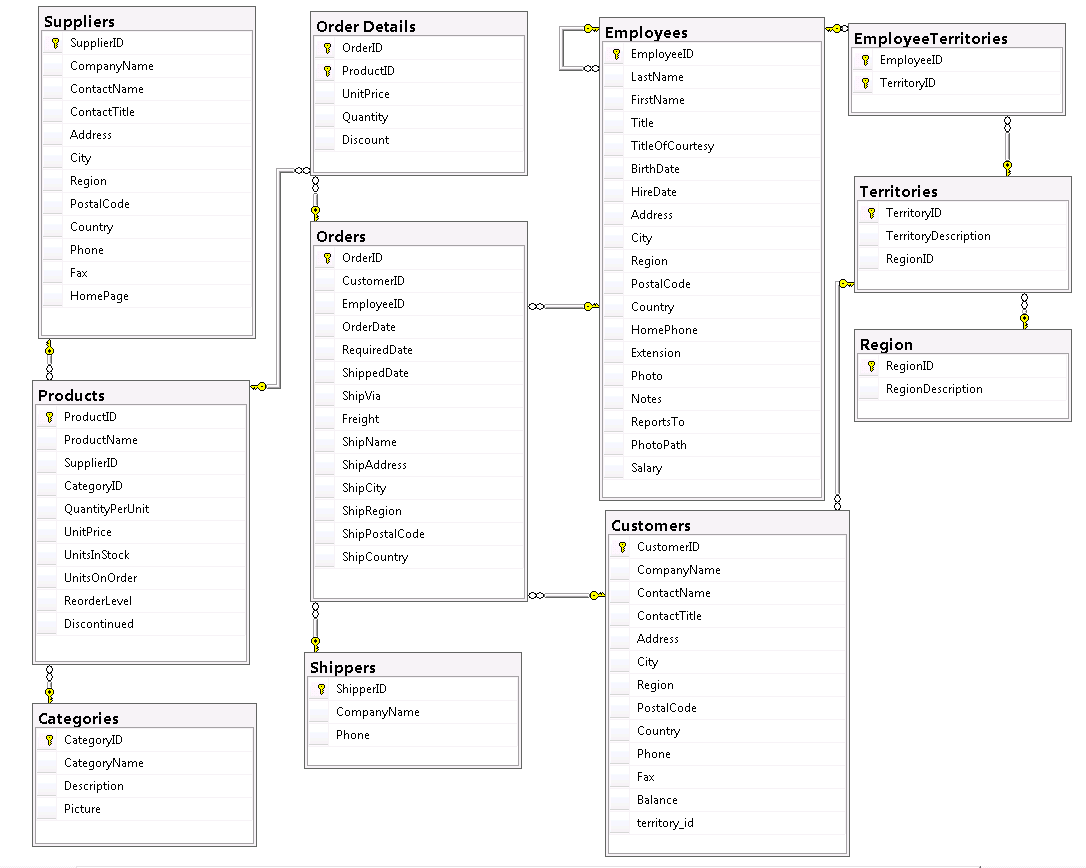
\includegraphics[width=0.75\linewidth,height=\textheight,keepaspectratio]{./images/img-005-002.png}

\begin{itemize}
\item
  A kiindulópontunk a \textbf{fogalmi modell} (tartománymodell vagy
  egyed-kapcsolat modell), amelyet a használati esetekből (use case)
  vezetünk le; célunk a logikai adatbázis-modell kidolgozása.
\item
  A \textbf{relációs modell} a legelterjedtebb paradigma a hagyományos
  üzleti folyamatok modellezésére, egyszerűsége miatt.
\item
  Az entitásokat, attribútumokat, példányokat és azonosítókat a relációs
  modellben táblák, mezők, rekordok és elsődleges kulcsok valósítják
  meg. A kulcsok több mezőből is állhatnak.
\item
  Minden cellában csak egyetlen érték szerepelhet; a harmadik
  normálforma (3NF) célja a redundancia és az inkonzisztencia
  minimalizálása. A 3NF jellemzői:

  \begin{itemize}
  \tightlist
  \item
    Minden táblának van egy elsődleges kulcsa, amely több mezőből is
    állhat, és amelytől az összes többi mező funkcionálisan függ.
  \item
    Összetett (többmezős) kulcsok esetén az összes nem-kulcs mező a
    teljes kulcstól függ, nem csupán annak egy részétől --- vagyis
    nincsenek \textbf{részleges függések}.
  \item
    A nem-kulcs mezők kizárólag a kulcstól függnek, más mezőtől nem ---
    vagyis nincs \textbf{tranzitív függés} a táblán belül.
  \end{itemize}
\item
  A táblák kapcsolatokon keresztül kapcsolódnak egymáshoz.
\item
  \textbf{1:N} (egy-a-sokhoz) kapcsolatokat idegen kulcsok valósítanak
  meg (pl. \texttt{Orders.EmployeeID}).
\item
  \textbf{N:M} (sok-a-sokhoz) kapcsolatokat kapcsolótáblák valósítanak
  meg (pl. \texttt{EmployeeTerritories}).
\item
  \textbf{1:1} (egy-az-egyhez) kapcsolatra a Northwind adatbázisban
  nincs példa.

  \begin{itemize}
  \tightlist
  \item
    Normál 1:1 kapcsolat lehet például egy \texttt{CompanyCar} tábla,
    ahol egy alkalmazotthoz legfeljebb egy céges autó tartozhat.
  \item
    Specializációs 1:1 kapcsolat lehet például egy
    \texttt{ExciseProducts} (Jövedéki termékek) tábla,
    \texttt{ExciseDutyAmount}, \texttt{RegBarCode} stb. extra mezőkkel.
  \end{itemize}
\item
  A kapcsolótábláknak általában összetett kulcsuk van. Mesterséges
  (generált) kulcsot csak akkor alkalmazunk, ha külső hivatkozás
  szükséges.
\item
  Az OLTP séma kapcsolatstruktúrája feltárja az adatbázist használó
  alkalmazás kulcstranzakcióit.

  \begin{itemize}
  \tightlist
  \item
    \textbf{Hópehely- (snowflake) vagy snowball struktúra}: minden
    hópehely egy vagy több tranzakciót szolgál ki.
  \item
    Az \textbf{alaptáblák} a leveleken helyezkednek el (pl.
    \texttt{Region}, \texttt{Customers}, \texttt{Categories}).
  \item
    A \textbf{tranzakciós táblák} (eseménytáblák) középen találhatók
    (\texttt{Order\ Details}, \texttt{EmployeeTerritories}). Ezek a
    táblák az információs rendszer „lüktető szívét'' alkotják.
  \end{itemize}
\end{itemize}

\begin{longtable}[]{@{}
  >{\raggedright\arraybackslash}p{(\linewidth - 4\tabcolsep) * \real{0.1407}}
  >{\raggedright\arraybackslash}p{(\linewidth - 4\tabcolsep) * \real{0.3630}}
  >{\raggedright\arraybackslash}p{(\linewidth - 4\tabcolsep) * \real{0.4963}}@{}}
\toprule\noalign{}
\begin{minipage}[b]{\linewidth}\raggedright
Jellemző
\end{minipage} & \begin{minipage}[b]{\linewidth}\raggedright
Alaptáblák
\end{minipage} & \begin{minipage}[b]{\linewidth}\raggedright
Tranzakciós táblák
\end{minipage} \\
\midrule\noalign{}
\endhead
\bottomrule\noalign{}
\endlastfoot
Pozíció a sémában & Levélelem. Nem hivatkozik más táblára. & Középpont.
Közvetlenül vagy közvetve hivatkozik az összes táblára. \\
Méret & Kicsi & Nagy \\
Változás sebessége & Lassú. Hideg (offline) mentés is elegendő lehet. &
Gyors. Online mentés szükséges. \\
\end{longtable}

\begin{itemize}
\item
  Megfeleltetés egy jól tervezett grafikus felhasználói felület (GUI) és
  a relációs séma között:

  \begin{itemize}
  \tightlist
  \item
    Rejtett vagy csak olvasható felirat: \textbf{kulcs}
  \item
    Szerkeszthető szövegmezők: a kulcstól függő attribútumok (mezők)
  \item
    Legördülő / kombinált listák: hivatkozások alaptáblákra
  \item
    Jelölőnégyzet kiegészítő szövegmezővel: specializáció
  \item
    Legördülő táblák vagy listák: 1:N kapcsolatok
  \end{itemize}
\item
  További olvasnivaló az adatmodellezésről:

  \begin{itemize}
  \tightlist
  \item
    https://www.safaribooksonline.com/library/view/relational-theory-for/9781449365431/ch01.html
  \item
    http://www.blackwasp.co.uk/RelationalDBConcepts.aspx
  \item
    https://www.tutorialspoint.com/ms\_sql\_server/index.htm
  \end{itemize}
\item
  \textbf{GYAKORLAT:} Hozd létre és bővítsd ki a mintaadatbázist!

  \begin{itemize}
  \item
    Telepítsd az MS SQL Server 2016-os vagy újabb verzióját, indítsd el
    az adatbázis-szolgáltatást, és csatlakozz hozzá az MS Management
    Studio segítségével.
  \item
    Futtasd a Northwind adatbázis-létrehozó szkriptjét (dump), és
    tekintsd át a táblákat a grafikus felhasználói felület (GUI)
    eszközeinek segítségével.
  \item
    Rajzolj a fenti diagramhoz hasonló logikai adatbázis-modell
    diagramot.
  \item
    Add hozzá az \texttt{Employees.Salary} és a
    \texttt{Customers.territory\_id} mezőket.
  \item
    Tervezd meg és valósítsd meg az adatbázis alábbi forgatókönyv
    modellezéséhez szükséges bővítményét:

    \begin{quote}
    \emph{Az alkalmazottainkat rendszeres képzésekre küldjük, ahol
    különböző készségeket sajátítanak el. A képzéseket szerződött
    harmadik fél cégek szervezik. Minden foglalkoztatási kategóriához
    (pl. „értékesítési vezető'', lásd \texttt{Employees.Title}) van egy
    listánk az elvárt készségekről (pl. „B szintű üzleti prezentáció''
    vagy „számviteli alapismeretek''), amelyeket a munkaviszony
    megkezdésétől számított 10 éven belül kell elsajátítani. Minden
    képzéshez tároljuk az időtartamot (kezdési és befejezési dátum), a
    helyszínt, a szervező céget, az oktatott készségeket, a
    résztvevőket, a képzési állapotukat (pl. „beiratkozott'',
    „elkezdett'', „befejezett'', „megszakított'') és vizsgaeredményeiket
    az egyes készségek vonatkozásában. A képzéseket szervező cégek
    tekintetében tároljuk a cégünk által az egyes képzési
    foglalkozásokért évente fizetett díjakat.}
    \end{quote}
  \item
    Add hozzá az új táblákat az adatbázis-diagramhoz, és vigyél fel
    néhány tesztadatot.
  \item
    MEGOLDÁS: \texttt{train\_tables.sql}²
  \end{itemize}
\end{itemize}

\begin{center}\rule{0.5\linewidth}{0.5pt}\end{center}

\subsection{Lekérdezés}\label{lekuxe9rdezuxe9s}

\begin{itemize}
\tightlist
\item
  Az SQL lekérdezés alapjait tekintjük át: adat-kiválasztás (select),
  csoportosítás, összekapcsolás (\texttt{join}). Példalekérdezések:

  \begin{itemize}
  \tightlist
  \item
    Az egyes rendelések értéke
  \item
    Az egyes termékekből évenként eladott minimális és maximális
    mennyiség
  \item
    Melyik alkalmazott adta el a legtöbb darabot a legnépszerűbb
    termékből 1998-ban?
  \end{itemize}
\end{itemize}

\begin{Shaded}
\begin{Highlighting}[]
\CommentTok{{-}{-} Az egyes rendelések értéke}
\KeywordTok{select}\NormalTok{ o.orderid, o.orderdate,}
\NormalTok{  str(}\FunctionTok{sum}\NormalTok{((}\DecValTok{1}\OperatorTok{{-}}\NormalTok{discount)}\OperatorTok{*}\NormalTok{unitprice}\OperatorTok{*}\NormalTok{quantity), }\DecValTok{15}\NormalTok{, }\DecValTok{2}\NormalTok{) }\KeywordTok{as}\NormalTok{ order\_value,}
  \FunctionTok{sum}\NormalTok{(quantity) }\KeywordTok{as}\NormalTok{ no\_of\_pieces,}
  \FunctionTok{count}\NormalTok{(d.orderid) }\KeywordTok{as}\NormalTok{ no\_of\_items}
\KeywordTok{from}\NormalTok{ orders o }\KeywordTok{inner} \KeywordTok{join}\NormalTok{ [}\KeywordTok{order}\NormalTok{ details] d }\KeywordTok{on}\NormalTok{ o.orderid}\OperatorTok{=}\NormalTok{d.orderid}
\KeywordTok{group} \KeywordTok{by}\NormalTok{ o.orderid, o.orderdate}
\KeywordTok{order} \KeywordTok{by} \FunctionTok{sum}\NormalTok{((}\DecValTok{1}\OperatorTok{{-}}\NormalTok{discount)}\OperatorTok{*}\NormalTok{unitprice}\OperatorTok{*}\NormalTok{quantity) }\KeywordTok{desc}

\CommentTok{{-}{-} Évenként eladott mennyiség termékenkénti bontásban}
\KeywordTok{select}\NormalTok{ p.ProductID, p.ProductName, }\DataTypeTok{year}\NormalTok{(o.orderdate), }\FunctionTok{SUM}\NormalTok{(quantity) }\KeywordTok{as}\NormalTok{ quantity}
\KeywordTok{from}\NormalTok{ orders o }\KeywordTok{inner} \KeywordTok{join}\NormalTok{ [}\KeywordTok{order}\NormalTok{ details] d }\KeywordTok{on}\NormalTok{ o.orderid}\OperatorTok{=}\NormalTok{d.orderid}
\KeywordTok{inner} \KeywordTok{join}\NormalTok{ Products p }\KeywordTok{on}\NormalTok{ p.ProductID}\OperatorTok{=}\NormalTok{d.ProductID}
\KeywordTok{group} \KeywordTok{by}\NormalTok{ p.ProductID, p.ProductName, }\DataTypeTok{year}\NormalTok{(o.orderdate)}
\KeywordTok{order} \KeywordTok{by}\NormalTok{ p.ProductName}

\CommentTok{{-}{-} Melyik alkalmazott adta el a legtöbb darabot a legnépszerűbb termékből 1998{-}ban?}
\KeywordTok{select}\NormalTok{ top }\DecValTok{1}\NormalTok{ u.titleofcourtesy}\OperatorTok{+}\StringTok{\textquotesingle{} \textquotesingle{}}\OperatorTok{+}\NormalTok{u.lastname}\OperatorTok{+}\StringTok{\textquotesingle{} \textquotesingle{}}\OperatorTok{+}\NormalTok{u.firstname}\OperatorTok{+}\StringTok{\textquotesingle{} (\textquotesingle{}}\OperatorTok{+}\NormalTok{u.title}\OperatorTok{+}\StringTok{\textquotesingle{})\textquotesingle{}} \KeywordTok{as}\NormalTok{ name,}
  \FunctionTok{sum}\NormalTok{(quantity) }\KeywordTok{as}\NormalTok{ pieces\_sold,}
\NormalTok{  pr.productname }\KeywordTok{as}\NormalTok{ productname}
\KeywordTok{from}\NormalTok{ orders o }\KeywordTok{inner} \KeywordTok{join}\NormalTok{ [}\KeywordTok{order}\NormalTok{ details] d }\KeywordTok{on}\NormalTok{ o.orderid}\OperatorTok{=}\NormalTok{d.orderid}
  \KeywordTok{inner} \KeywordTok{join}\NormalTok{ employees u }\KeywordTok{on}\NormalTok{ u.employeeid}\OperatorTok{=}\NormalTok{o.employeeid}
  \KeywordTok{inner} \KeywordTok{join}\NormalTok{ products pr }\KeywordTok{on}\NormalTok{ pr.productid}\OperatorTok{=}\NormalTok{d.productid}
\KeywordTok{where} \DataTypeTok{year}\NormalTok{(o.orderdate)}\OperatorTok{=}\DecValTok{1998} \KeywordTok{and}\NormalTok{ d.productid }\OperatorTok{=}
\NormalTok{  (}\KeywordTok{select}\NormalTok{ top }\DecValTok{1}\NormalTok{ p.productid}
  \KeywordTok{from}\NormalTok{ products p }\KeywordTok{left} \KeywordTok{outer} \KeywordTok{join}\NormalTok{ [}\KeywordTok{order}\NormalTok{ details] d }\KeywordTok{on}\NormalTok{ p.productid}\OperatorTok{=}\NormalTok{d.productid}
  \KeywordTok{group} \KeywordTok{by}\NormalTok{ p.productid}
  \KeywordTok{order} \KeywordTok{by} \FunctionTok{count}\NormalTok{(}\OperatorTok{*}\NormalTok{) }\KeywordTok{desc}\NormalTok{)}
\KeywordTok{group} \KeywordTok{by}\NormalTok{ u.employeeid, u.titleofcourtesy, u.title, u.lastname, u.firstname,}
\NormalTok{pr.ProductID, pr.productname}
\KeywordTok{order} \KeywordTok{by} \FunctionTok{sum}\NormalTok{(quantity) }\KeywordTok{desc}
\end{Highlighting}
\end{Shaded}

\begin{itemize}
\item
  További példákért és az SQL lekérdezések szisztematikus áttekintéséért
  lásd a Mellékletet.
\item
  További olvasnivaló a lekérdezésekről:

  \begin{itemize}
  \tightlist
  \item
    https://docs.microsoft.com/en-us/sql/t-sql/queries/queries
  \end{itemize}
\item
  \textbf{GYAKORLAT:} Az első gyakorlatban megvalósított táblák
  segítségével valósítsd meg a következő lekérdezéseket:

  \begin{itemize}
  \tightlist
  \item
    Mik a hiányzó készségek Mrs.~Peacock számára?
  \item
    Vannak-e olyan jövőbeli képzések, amelyeken Peacocknak még részt
    kell vennie?
  \item
    Mi az első és az utolsó képzési dátum, és mekkora a képzések átlagos
    időtartama napokban?
  \item
    Melyik alkalmazott rendelkezik a legtöbb olyan készséggel, amelynek
    vizsgaeredménye jobb, mint „nem felelt meg'' (fail)?
  \item
    Mennyi az összes díj, amelyet azokért a képzési foglalkozásokért
    fizettünk, amelyeken a legképzettebb alkalmazottunk (lásd fent)
    részt vett?
  \item
    Melyik elvárt készség(ek)et nem fedte le még egyetlen képzési
    foglalkozás sem?
  \item
    MEGOLDÁS: \texttt{train\_solution.sql}
  \end{itemize}
\end{itemize}

\begin{center}\rule{0.5\linewidth}{0.5pt}\end{center}

\subsection{Programozás}\label{programozuxe1s}

\begin{itemize}
\item
  A deklaratív SQL lekérdezések mellett a procedurális üzleti logika a
  T-SQL szkriptnyelvben is megvalósítható, és a szerveroldalon
  futtatható és tárolható.

  \begin{itemize}
  \item
    A szerveroldali üzleti logika előnyei és hátrányai:

    \begin{itemize}
    \tightlist
    \item
      ✓ Egyszerű architektúra
    \item
      ✓ Platformfüggetlenség
    \item
      ✓ Adatbiztonság
    \item
      ✓ Kezelhetőség
    \item
      ✓ Hatékonyság
    \item
      ✓ Jól olvasható kód
    \item
      ✗ Alacsony szintű
    \item
      ✗ Gyenge szoftvertechnológiai támogatás
    \item
      ✗ Drága skálázhatóság
    \end{itemize}
  \item
    Összefoglalás: azokat az üzletilogika-elemeket, amelyek \emph{nagy
    mennyiségű}, \emph{strukturált} adaton végzett egyszerű, halmazalapú
    műveleteket igényelnek, a legjobb az adatbázis-szerveren tárolt
    eljárások, függvények, triggerek és ütemezett feladatok formájában
    megvalósítani. A procedurálisan összetett részeket, amelyekhez magas
    szintű, objektumorientált programozási környezet szükséges,
    alkalmazásszerveren kell futtatni.
  \item
    A szerveroldali programozhatóság elemei:

    \begin{itemize}
    \tightlist
    \item
      Speciális SQL vezérlőutasítások: \texttt{DECLARE}, \texttt{SET},
      \texttt{BEGIN/END}, \texttt{IF/ELSE},
      \texttt{WHILE/BREAK/CONTINUE}, \texttt{RETURN},
      \texttt{WAITFOR/DELAY/TIME}, \texttt{GOTO}
    \item
      Hibakezelés: \texttt{TRY/CATCH/THROW/RAISERROR}
    \item
      Programozhatóságot támogató objektumok:
      \texttt{CREATE\ PROCEDURE/FUNCTION/TRIGGER}
    \item
      Tranzakciókezelés: \texttt{BEGIN/COMMIT/ROLLBACK\ TRANSACTION}
    \end{itemize}
  \item
    Az alábbiakban egy egyszerű T-SQL szkript és tárolt eljárásként
    megvalósított megfelelője látható. A hasonló, felhasználó által
    definiált függvény \texttt{SELECT} utasításban is hívható.
  \end{itemize}
\end{itemize}

\begin{Shaded}
\begin{Highlighting}[]
\CommentTok{{-}{-}egyszerű szkript: alkalmazott keresése, és ha egyetlen egyező rekordot találunk,}
\CommentTok{{-}{-}a fizetés emelése 10\%{-}kal}
\KeywordTok{set}\NormalTok{ nocount }\KeywordTok{on}
\KeywordTok{declare}\NormalTok{ @name }\DataTypeTok{nvarchar}\NormalTok{(}\DecValTok{20}\NormalTok{), @address }\DataTypeTok{nvarchar}\NormalTok{(}\FunctionTok{max}\NormalTok{), @res\_no }\DataTypeTok{int}\NormalTok{, @emp\_id }\DataTypeTok{int}
\KeywordTok{set}\NormalTok{ @name}\OperatorTok{=}\StringTok{\textquotesingle{}Fuller\textquotesingle{}}
\KeywordTok{select}\NormalTok{ @res\_no}\OperatorTok{=}\FunctionTok{count}\NormalTok{(}\OperatorTok{*}\NormalTok{) }\KeywordTok{from}\NormalTok{ Employees }\KeywordTok{where}\NormalTok{ LastName }\KeywordTok{like}\NormalTok{ @name }\OperatorTok{+} \StringTok{\textquotesingle{}\%\textquotesingle{}}
\ControlFlowTok{if}\NormalTok{ @res\_no}\OperatorTok{=}\DecValTok{0}\NormalTok{ print }\StringTok{\textquotesingle{}No matching record.\textquotesingle{}}
\ControlFlowTok{else} \ControlFlowTok{if}\NormalTok{ @res\_no}\OperatorTok{\textgreater{}}\DecValTok{1}\NormalTok{ print }\StringTok{\textquotesingle{}More than one matching record.\textquotesingle{}}
\ControlFlowTok{else} \ControlFlowTok{begin} \CommentTok{{-}{-}egyetlen találat}
    \KeywordTok{select}\NormalTok{ @address}\OperatorTok{=}\NormalTok{Country}\OperatorTok{+}\StringTok{\textquotesingle{}, \textquotesingle{}}\OperatorTok{+}\NormalTok{City}\OperatorTok{+}\StringTok{\textquotesingle{} \textquotesingle{}}\OperatorTok{+}\NormalTok{Address, @emp\_id}\OperatorTok{=}\NormalTok{EmployeeID}
        \KeywordTok{from}\NormalTok{ Employees }\KeywordTok{where}\NormalTok{ LastName }\KeywordTok{like}\NormalTok{ @name}
\NormalTok{    print }\StringTok{\textquotesingle{}Employee ID: \textquotesingle{}} \OperatorTok{+} \FunctionTok{cast}\NormalTok{(@emp\_id }\KeywordTok{as} \DataTypeTok{varchar}\NormalTok{(}\DecValTok{10}\NormalTok{)) }\OperatorTok{+} \StringTok{\textquotesingle{}, address: \textquotesingle{}} \OperatorTok{+}\NormalTok{ @address}
    \KeywordTok{update}\NormalTok{ Employees }\KeywordTok{set}\NormalTok{ salary}\OperatorTok{=}\FloatTok{1.1}\OperatorTok{*}\NormalTok{salary }\KeywordTok{where}\NormalTok{ EmployeeID}\OperatorTok{=}\NormalTok{@emp\_id}
\NormalTok{    print }\StringTok{\textquotesingle{}Salary increased.\textquotesingle{}}
\ControlFlowTok{end}
\NormalTok{go}

\CommentTok{{-}{-}tárolt eljárásba csomagolva}
\KeywordTok{create} \KeywordTok{procedure}\NormalTok{ sp\_increase\_salary @name }\DataTypeTok{nvarchar}\NormalTok{(}\DecValTok{40}\NormalTok{)}
\KeywordTok{as}
\KeywordTok{set}\NormalTok{ nocount }\KeywordTok{on}
\KeywordTok{declare}\NormalTok{ @address }\DataTypeTok{nvarchar}\NormalTok{(}\FunctionTok{max}\NormalTok{), @res\_no }\DataTypeTok{int}\NormalTok{, @emp\_id }\DataTypeTok{int}
\KeywordTok{select}\NormalTok{ @res\_no}\OperatorTok{=}\FunctionTok{count}\NormalTok{(}\OperatorTok{*}\NormalTok{) }\KeywordTok{from}\NormalTok{ Employees }\KeywordTok{where}\NormalTok{ LastName }\KeywordTok{like}\NormalTok{ @name }\OperatorTok{+} \StringTok{\textquotesingle{}\%\textquotesingle{}}
\ControlFlowTok{if}\NormalTok{ @res\_no}\OperatorTok{=}\DecValTok{0}\NormalTok{ print }\StringTok{\textquotesingle{}No matching record.\textquotesingle{}}
\ControlFlowTok{else} \ControlFlowTok{if}\NormalTok{ @res\_no}\OperatorTok{\textgreater{}}\DecValTok{1}\NormalTok{ print }\StringTok{\textquotesingle{}More than one matching record.\textquotesingle{}}
\ControlFlowTok{else} \ControlFlowTok{begin} \CommentTok{{-}{-}egyetlen találat}
    \KeywordTok{select}\NormalTok{ @address}\OperatorTok{=}\NormalTok{Country}\OperatorTok{+}\StringTok{\textquotesingle{}, \textquotesingle{}}\OperatorTok{+}\NormalTok{City}\OperatorTok{+}\StringTok{\textquotesingle{} \textquotesingle{}}\OperatorTok{+}\NormalTok{Address, @emp\_id}\OperatorTok{=}\NormalTok{EmployeeID}
        \KeywordTok{from}\NormalTok{ Employees }\KeywordTok{where}\NormalTok{ LastName }\KeywordTok{like}\NormalTok{ @name}
\NormalTok{    print }\StringTok{\textquotesingle{}Employee ID: \textquotesingle{}} \OperatorTok{+} \FunctionTok{cast}\NormalTok{(@emp\_id }\KeywordTok{as} \DataTypeTok{varchar}\NormalTok{(}\DecValTok{10}\NormalTok{)) }\OperatorTok{+} \StringTok{\textquotesingle{}, address: \textquotesingle{}} \OperatorTok{+}\NormalTok{ @address}
    \KeywordTok{update}\NormalTok{ Employees }\KeywordTok{set}\NormalTok{ salary}\OperatorTok{=}\FloatTok{1.1}\OperatorTok{*}\NormalTok{salary }\KeywordTok{where}\NormalTok{ EmployeeID}\OperatorTok{=}\NormalTok{@emp\_id}
\NormalTok{    print }\StringTok{\textquotesingle{}Salary increased.\textquotesingle{}}
\ControlFlowTok{end}
\NormalTok{go}
\CommentTok{{-}{-}teszt}
\KeywordTok{select}\NormalTok{ Salary }\KeywordTok{from}\NormalTok{ Employees }\KeywordTok{where}\NormalTok{ LastName }\KeywordTok{like} \StringTok{\textquotesingle{}Fuller\%\textquotesingle{}}
\KeywordTok{exec}\NormalTok{ sp\_increase\_salary }\StringTok{\textquotesingle{}Fuller\textquotesingle{}}
\KeywordTok{select}\NormalTok{ Salary }\KeywordTok{from}\NormalTok{ Employees }\KeywordTok{where}\NormalTok{ LastName }\KeywordTok{like} \StringTok{\textquotesingle{}Fuller\%\textquotesingle{}}

\CommentTok{{-}{-}skaláris értékű függvény: visszaadja egy személy fizetését, vagy 0{-}t, ha nem található}
\NormalTok{go}
\KeywordTok{create} \KeywordTok{function}\NormalTok{ fn\_salary (@name }\DataTypeTok{nvarchar}\NormalTok{(}\DecValTok{40}\NormalTok{)) returns money }\KeywordTok{as}
\ControlFlowTok{begin}
    \KeywordTok{declare}\NormalTok{ @salary money, @res\_no }\DataTypeTok{int}
    \KeywordTok{select}\NormalTok{ @res\_no}\OperatorTok{=}\FunctionTok{count}\NormalTok{(}\OperatorTok{*}\NormalTok{) }\KeywordTok{from}\NormalTok{ Employees }\KeywordTok{where}\NormalTok{ LastName }\KeywordTok{like}\NormalTok{ @name }\OperatorTok{+} \StringTok{\textquotesingle{}\%\textquotesingle{}}
    \ControlFlowTok{if}\NormalTok{ @res\_no }\OperatorTok{\textless{}\textgreater{}} \DecValTok{1} \KeywordTok{set}\NormalTok{ @salary}\OperatorTok{=}\DecValTok{0}
    \ControlFlowTok{else} \KeywordTok{select}\NormalTok{ @salary}\OperatorTok{=}\NormalTok{Salary }\KeywordTok{from}\NormalTok{ Employees }\KeywordTok{where}\NormalTok{ LastName }\KeywordTok{like}\NormalTok{ @name }\OperatorTok{+} \StringTok{\textquotesingle{}\%\textquotesingle{}}
    \KeywordTok{return}\NormalTok{ @salary}
\ControlFlowTok{end}
\NormalTok{go}
\CommentTok{{-}{-}teszt}
\KeywordTok{select}\NormalTok{ [your }\FunctionTok{user}\NormalTok{ name].fn\_salary(}\StringTok{\textquotesingle{}Fuller\textquotesingle{}}\NormalTok{) }\KeywordTok{as}\NormalTok{ salary}
\end{Highlighting}
\end{Shaded}

\begin{itemize}
\item
  Megjegyzés: a \textbf{tárolt eljárás} több rekordhalmazt is
  visszaadhat, ha változóhozzárendelés nélkül több \texttt{SELECT}
  utasítást tartalmaz. A fenti példában szereplő paraméterek INPUT
  típusú paraméterek. A tárolt eljárások OUTPUT paraméterekkel skaláris
  értékeket is visszaadhatnak (nem szerepel a példában). Mivel más
  tárolt eljárásokat és függvényeket is meghívhatnak, összetett üzleti
  logika is megvalósítható velük az adatbázis-szerveren.
\item
  A \textbf{felhasználó által definiált függvény} abban különbözik a
  tárolt eljárástól, hogy egyetlen visszatérési értéke van --- típusa
  skaláris (pl. \texttt{money}) vagy tábla lehet. A függvény utolsó
  utasítása \texttt{RETURN} kell legyen. A felhasználó által definiált
  függvények előnye, hogy \texttt{SELECT} utasításból is meghívhatók,
  akárcsak a beépített SQL függvények (pl. \texttt{DATEDIFF}), így
  jelentősen növelik a statikus SQL lekérdezések rugalmasságát.
\item
  \textbf{GYAKORLAT:}

  \begin{itemize}
  \tightlist
  \item
    A képzési lekérdezések segítségével hozz létre egy tárolt eljárást,
    amely visszaadja a hiányzó készségeket egy paraméterként átadott
    alkalmazott neve alapján. Az eljárás egyetlen mezőt tartalmazó
    táblát adjon vissza. Ha az alkalmazott nem azonosítható
    egyértelműen, adj vissza hibaüzenetet, és ne adj vissza táblát.
  \item
    A képzési lekérdezések segítségével hozz létre egy tábla értékű
    függvényt, amely egy \texttt{employeeID} alapján adja vissza a
    hiányzó készségeket. Tipp: használd a \texttt{returns\ table}
    kulcsszót a függvény specifikációjában.
  \end{itemize}
\item
  Egy reálisabb üzleti folyamat bemutatásához lássunk egy
  példaszkriptet, amely egy új Northwind rendelést hoz létre egyetlen
  rendelési tétellel. A forgatókönyv: a vállalat irodája telefonon
  sürgős rendelést kap egy értékes vevőtől --- ez egy tipikus üzleti
  tranzakció.
\end{itemize}

\begin{Shaded}
\begin{Highlighting}[]
\CommentTok{{-}{-}változók}
\KeywordTok{declare}\NormalTok{ @prod\_name }\DataTypeTok{varchar}\NormalTok{(}\DecValTok{20}\NormalTok{), @quantity }\DataTypeTok{int}\NormalTok{, @cust\_id }\DataTypeTok{nchar}\NormalTok{(}\DecValTok{5}\NormalTok{)}
\KeywordTok{declare}\NormalTok{ @status\_message }\DataTypeTok{nvarchar}\NormalTok{(}\DecValTok{100}\NormalTok{), @status }\DataTypeTok{int}
\KeywordTok{declare}\NormalTok{ @res\_no }\DataTypeTok{int}
\KeywordTok{declare}\NormalTok{ @prod\_id }\DataTypeTok{int}\NormalTok{, @order\_id }\DataTypeTok{int}
\KeywordTok{declare}\NormalTok{ @stock }\DataTypeTok{int}
\KeywordTok{declare}\NormalTok{ @cust\_balance money}
\KeywordTok{declare}\NormalTok{ @unitprice money}

\CommentTok{{-}{-} paraméterek}
\KeywordTok{set}\NormalTok{ @prod\_name }\OperatorTok{=} \StringTok{\textquotesingle{}boston\textquotesingle{}}
\KeywordTok{set}\NormalTok{ @quantity }\OperatorTok{=} \DecValTok{10}
\KeywordTok{set}\NormalTok{ @cust\_id }\OperatorTok{=} \StringTok{\textquotesingle{}AROUT\textquotesingle{}}

\ControlFlowTok{begin}\NormalTok{ try}
  \KeywordTok{select}\NormalTok{ @res\_no }\OperatorTok{=} \FunctionTok{count}\NormalTok{(}\OperatorTok{*}\NormalTok{) }\KeywordTok{from}\NormalTok{ products }\KeywordTok{where}\NormalTok{ productname }\KeywordTok{like} \StringTok{\textquotesingle{}\%\textquotesingle{}} \OperatorTok{+}\NormalTok{ @prod\_name }\OperatorTok{+} \StringTok{\textquotesingle{}\%\textquotesingle{}}
  \ControlFlowTok{if}\NormalTok{ @res\_no }\OperatorTok{\textless{}\textgreater{}} \DecValTok{1} \ControlFlowTok{begin}
      \KeywordTok{set}\NormalTok{ @status }\OperatorTok{=} \DecValTok{1}
      \KeywordTok{set}\NormalTok{ @status\_message }\OperatorTok{=} \StringTok{\textquotesingle{}ERROR: Ambiguous Product name.\textquotesingle{}}\NormalTok{;}
  \ControlFlowTok{end} \ControlFlowTok{else} \ControlFlowTok{begin}
      \KeywordTok{select}\NormalTok{ @prod\_id }\OperatorTok{=}\NormalTok{ productID, @stock }\OperatorTok{=}\NormalTok{ unitsInStock }\KeywordTok{from}\NormalTok{ products }\KeywordTok{where}
\NormalTok{productName }\KeywordTok{like} \StringTok{\textquotesingle{}\%\textquotesingle{}} \OperatorTok{+}\NormalTok{ @prod\_name }\OperatorTok{+} \StringTok{\textquotesingle{}\%\textquotesingle{}}
      \ControlFlowTok{if}\NormalTok{ @stock }\OperatorTok{\textless{}}\NormalTok{ @quantity }\ControlFlowTok{begin}
          \KeywordTok{set}\NormalTok{ @status }\OperatorTok{=} \DecValTok{2}
          \KeywordTok{set}\NormalTok{ @status\_message }\OperatorTok{=} \StringTok{\textquotesingle{}ERROR: Stock is insufficient.\textquotesingle{}}
      \ControlFlowTok{end} \ControlFlowTok{else} \ControlFlowTok{begin}
          \KeywordTok{select}\NormalTok{ @cust\_balance }\OperatorTok{=}\NormalTok{ balance }\KeywordTok{from}\NormalTok{ customers }\KeywordTok{where}\NormalTok{ customerid }\OperatorTok{=}\NormalTok{ @cust\_id}
          \KeywordTok{select}\NormalTok{ @unitprice }\OperatorTok{=}\NormalTok{ unitPrice }\KeywordTok{from}\NormalTok{ products }\KeywordTok{where}\NormalTok{ productID }\OperatorTok{=}\NormalTok{ @prod\_id}
          \ControlFlowTok{if}\NormalTok{ @cust\_balance }\OperatorTok{\textless{}}\NormalTok{ @quantity}\OperatorTok{*}\NormalTok{@unitprice }\KeywordTok{or}\NormalTok{ @cust\_balance }\KeywordTok{is} \KeywordTok{null}
          \ControlFlowTok{begin}
              \KeywordTok{set}\NormalTok{ @status }\OperatorTok{=} \DecValTok{3}
              \KeywordTok{set}\NormalTok{ @status\_message }\OperatorTok{=} \StringTok{\textquotesingle{}ERROR: Customer not found or balance insufficient.\textquotesingle{}}
          \ControlFlowTok{end} \ControlFlowTok{else} \ControlFlowTok{begin}
              \CommentTok{{-}{-} nincs több ellenőrzés, kezdjük a tranzakciót (3 lépés)}
              \CommentTok{{-}{-} 1. egyenleg csökkentése}
              \KeywordTok{update}\NormalTok{ customers }\KeywordTok{set}\NormalTok{ balance }\OperatorTok{=}\NormalTok{ balance}\OperatorTok{{-}}\NormalTok{(@quantity}\OperatorTok{*}\NormalTok{@unitprice) }\KeywordTok{where}
\NormalTok{customerid}\OperatorTok{=}\NormalTok{@cust\_id}
              \CommentTok{{-}{-} 2. új rekord az Orders és Order Details táblákban}
              \KeywordTok{insert} \KeywordTok{into}\NormalTok{ orders (customerID, orderdate) }\KeywordTok{values}\NormalTok{ (@cust\_id, getdate())}
              \KeywordTok{set}\NormalTok{ @order\_id }\OperatorTok{=}\NormalTok{ @@identity}
              \KeywordTok{insert}\NormalTok{ [}\KeywordTok{order}\NormalTok{ details] (orderid, productid, quantity,}
\NormalTok{UnitPrice, Discount) }\KeywordTok{values}\NormalTok{(@order\_id, @prod\_id, @quantity, @unitprice, }\DecValTok{0}\NormalTok{)}
              \CommentTok{{-}{-} 3. készlet frissítése}
              \KeywordTok{update}\NormalTok{ products }\KeywordTok{set}\NormalTok{ unitsInStock }\OperatorTok{=}\NormalTok{ unitsInStock }\OperatorTok{{-}}\NormalTok{ @quantity}
\KeywordTok{where}\NormalTok{ productid }\OperatorTok{=}\NormalTok{ @prod\_id}
              \KeywordTok{set}\NormalTok{ @status }\OperatorTok{=} \DecValTok{0}
              \KeywordTok{set}\NormalTok{ @status\_message }\OperatorTok{=} \StringTok{\textquotesingle{}Order No. \textquotesingle{}} \OperatorTok{+} \FunctionTok{cast}\NormalTok{(@order\_id }\KeywordTok{as} \DataTypeTok{varchar}\NormalTok{(}\DecValTok{20}\NormalTok{)) }\OperatorTok{+} \StringTok{\textquotesingle{} processed successfully.\textquotesingle{}}
          \ControlFlowTok{end}
      \ControlFlowTok{end}
  \ControlFlowTok{end}
\NormalTok{  print @status}
\NormalTok{  print @status\_message}
\ControlFlowTok{end}\NormalTok{ try}
\ControlFlowTok{begin}\NormalTok{ catch}
\NormalTok{  print }\StringTok{\textquotesingle{}OTHER ERROR: \textquotesingle{}}\OperatorTok{+}\NormalTok{ ERROR\_MESSAGE() }\OperatorTok{+} \StringTok{\textquotesingle{} (\textquotesingle{}} \OperatorTok{+} \FunctionTok{cast}\NormalTok{(ERROR\_NUMBER() }\KeywordTok{as} \DataTypeTok{varchar}\NormalTok{(}\DecValTok{20}\NormalTok{)) }\OperatorTok{+} \StringTok{\textquotesingle{})\textquotesingle{}}
\ControlFlowTok{end}\NormalTok{ catch}
\NormalTok{go}
\end{Highlighting}
\end{Shaded}

\begin{itemize}
\item
  Teszteld a fenti tárolt eljárást különböző hibákra: programozási hibák
  és logikai hibák (pl. elégtelen készlet). Ellenőrizd az adatbázis
  integritását. Győződj meg arról, hogy a tranzakciós támogatás
  megakadályozza a súlyos hibákat.
\item
  Az elszigeteltség biztosítása érdekében a szerver zárolást alkalmaz
  sorokon (rekordokon), tartományokon vagy táblákon. Az
  \textbf{izolációs szint} (Isolation Level) a szerver által
  kényszerített zárolási stratégia. Az MS SQL Server fő zártípusai:
  megosztott (shared), kizárólagos (exclusive) és frissítési (update). A
  négy ANSI szabványos izolációs szint:

  \begin{itemize}
  \tightlist
  \item
    \texttt{READ\ UNCOMMITTED}: nincs zárolás
  \item
    \texttt{READ\ COMMITTED}: a zárak az SQL utasítás végrehajtása után
    felszabadulnak
  \item
    \texttt{REPEATABLE\ READ}: a tranzakcióhoz kiosztott zárak a
    tranzakció végéig megmaradnak
  \item
    \texttt{SERIALIZABLE}: más tranzakciók nem szúrhatnak be rekordokat
    olyan táblába, amelyen a tranzakciónak sor- vagy tartományzárja van
    --- fantomolvasás nem lehetséges
  \end{itemize}
\end{itemize}

\begin{Shaded}
\begin{Highlighting}[]
\CommentTok{{-}{-}egyszerű izolációs szint bemutató: webáruház eset}
\KeywordTok{create} \KeywordTok{table}\NormalTok{ test\_product(}\KeywordTok{id} \DataTypeTok{int} \KeywordTok{primary} \KeywordTok{key}\NormalTok{, prod\_name }\DataTypeTok{varchar}\NormalTok{(}\DecValTok{50}\NormalTok{) }\KeywordTok{not} \KeywordTok{null}\NormalTok{, sold}
\DataTypeTok{varchar}\NormalTok{(}\DecValTok{50}\NormalTok{), buyer }\DataTypeTok{varchar}\NormalTok{(}\DecValTok{50}\NormalTok{))}
\KeywordTok{insert}\NormalTok{ test\_product(}\KeywordTok{id}\NormalTok{, prod\_name, sold) }\KeywordTok{values}\NormalTok{ (}\DecValTok{1}\NormalTok{, }\StringTok{\textquotesingle{}car\textquotesingle{}}\NormalTok{, }\StringTok{\textquotesingle{}for sale\textquotesingle{}}\NormalTok{)}
\KeywordTok{insert}\NormalTok{ test\_product(}\KeywordTok{id}\NormalTok{, prod\_name, sold) }\KeywordTok{values}\NormalTok{ (}\DecValTok{2}\NormalTok{, }\StringTok{\textquotesingle{}horse\textquotesingle{}}\NormalTok{, }\StringTok{\textquotesingle{}for sale\textquotesingle{}}\NormalTok{)}
\NormalTok{go}
\KeywordTok{set}\NormalTok{ tran }\KeywordTok{isolation} \KeywordTok{level} \KeywordTok{read} \KeywordTok{committed} \CommentTok{{-}{-}az alapértelmezett}
\NormalTok{go}
\ControlFlowTok{begin}\NormalTok{ tran}
\KeywordTok{declare}\NormalTok{ @sold }\DataTypeTok{varchar}\NormalTok{(}\DecValTok{50}\NormalTok{)}
\KeywordTok{select}\NormalTok{ @sold}\OperatorTok{=}\NormalTok{sold }\KeywordTok{from}\NormalTok{ test\_product }\KeywordTok{where} \KeywordTok{id}\OperatorTok{=}\DecValTok{2}
\ControlFlowTok{if}\NormalTok{ @sold}\OperatorTok{=}\StringTok{\textquotesingle{}for sale\textquotesingle{}} \ControlFlowTok{begin}
\NormalTok{  waitfor delay }\StringTok{\textquotesingle{}00:00:10\textquotesingle{}} \CommentTok{{-}{-}bankátutalás szimulálása}
  \KeywordTok{update}\NormalTok{ test\_product }\KeywordTok{set}\NormalTok{ sold}\OperatorTok{=}\StringTok{\textquotesingle{}sold\textquotesingle{}}\NormalTok{, buyer}\OperatorTok{=}\StringTok{\textquotesingle{}My name\textquotesingle{}} \KeywordTok{where} \KeywordTok{id}\OperatorTok{=}\DecValTok{2}
\NormalTok{  print }\StringTok{\textquotesingle{}sold successfully\textquotesingle{}}
\ControlFlowTok{end} \ControlFlowTok{else}\NormalTok{ print }\StringTok{\textquotesingle{}product not available\textquotesingle{}}
\KeywordTok{commit}\NormalTok{ tran}
\NormalTok{go}
\CommentTok{{-}{-}Következtetés: körültekintően válaszd meg a megfelelő izolációs szintet.}
\end{Highlighting}
\end{Shaded}

\begin{itemize}
\tightlist
\item
  \textbf{GYAKORLAT:} Az előző gyakorlatokban megvalósított táblák és
  szkriptek segítségével:

  \begin{itemize}
  \tightlist
  \item
    Írj egy szkriptet, amely ellenőrzi, hogy egy alkalmazottnak szüksége
    van-e valamelyik képzési foglalkozáson kínált készségre, és ha igen,
    iratkoztasd be az alkalmazottat az összes ilyen foglalkozásra.
  \item
    Futtasd a szkriptet tárolt eljárásként.
  \item
    MEGOLDÁS: \texttt{train\_solution.sql}
  \end{itemize}
\end{itemize}

\begin{center}\rule{0.5\linewidth}{0.5pt}\end{center}

\subsection{Kurzorok}\label{kurzorok}

A kurzorok olyan problémáknál alkalmazhatók, ahol a procedurális,
rekordonkénti feldolgozás megfelelőbb, mint a halmazalapú lekérdezési
megközelítés.

\textbf{PÉLDA} kurzor szintaxisra:

\begin{Shaded}
\begin{Highlighting}[]
\KeywordTok{declare}\NormalTok{ @emp\_id }\DataTypeTok{int}\NormalTok{, @emp\_name }\DataTypeTok{nvarchar}\NormalTok{(}\DecValTok{50}\NormalTok{), @i }\DataTypeTok{int}\NormalTok{, @address }\DataTypeTok{nvarchar}\NormalTok{(}\DecValTok{60}\NormalTok{)}
\KeywordTok{declare}\NormalTok{ cursor\_emp }\KeywordTok{cursor} \ControlFlowTok{for}
  \KeywordTok{select}\NormalTok{ employeeid, lastname, address }\KeywordTok{from}\NormalTok{ employees }\KeywordTok{order} \KeywordTok{by}\NormalTok{ lastname}
\KeywordTok{set}\NormalTok{ @i}\OperatorTok{=}\DecValTok{1}
\KeywordTok{open}\NormalTok{ cursor\_emp}
\NormalTok{fetch }\KeywordTok{next} \KeywordTok{from}\NormalTok{ cursor\_emp }\KeywordTok{into}\NormalTok{ @emp\_id, @emp\_name, @address}
\ControlFlowTok{while}\NormalTok{ @@fetch\_status }\OperatorTok{=} \DecValTok{0}
\ControlFlowTok{begin}
\NormalTok{  print }\FunctionTok{cast}\NormalTok{(@i }\KeywordTok{as} \DataTypeTok{varchar}\NormalTok{(}\DecValTok{5}\NormalTok{)) }\OperatorTok{+} \StringTok{\textquotesingle{} EMPLOYEE:\textquotesingle{}}
\NormalTok{  print }\StringTok{\textquotesingle{}ID: \textquotesingle{}} \OperatorTok{+} \FunctionTok{cast}\NormalTok{(@emp\_id }\KeywordTok{as} \DataTypeTok{varchar}\NormalTok{(}\DecValTok{5}\NormalTok{)) }\OperatorTok{+} \StringTok{\textquotesingle{}, LASTNAME: \textquotesingle{}} \OperatorTok{+}\NormalTok{ @emp\_name }\OperatorTok{+} \StringTok{\textquotesingle{}, ADDRESS: \textquotesingle{}} \OperatorTok{+}\NormalTok{ @address}
  \KeywordTok{set}\NormalTok{ @i}\OperatorTok{=}\NormalTok{@i}\OperatorTok{+}\DecValTok{1}
\NormalTok{  fetch }\KeywordTok{next} \KeywordTok{from}\NormalTok{ cursor\_emp }\KeywordTok{into}\NormalTok{ @emp\_id, @emp\_name, @address}
\ControlFlowTok{end}
\KeywordTok{close}\NormalTok{ cursor\_emp}
\KeywordTok{deallocate}\NormalTok{ cursor\_emp}
\NormalTok{go}
\CommentTok{{-}{-}ezzel egyenértékű SELECT megoldás}
\KeywordTok{select} \StringTok{\textquotesingle{}ID: \textquotesingle{}} \OperatorTok{+} \FunctionTok{cast}\NormalTok{(employeeid }\KeywordTok{as} \DataTypeTok{varchar}\NormalTok{(}\DecValTok{5}\NormalTok{)) }\OperatorTok{+}\NormalTok{ isnull(}\StringTok{\textquotesingle{}, LASTNAME: \textquotesingle{}} \OperatorTok{+}\NormalTok{ lastname, }\StringTok{\textquotesingle{}\textquotesingle{}}\NormalTok{) }\OperatorTok{+}
\NormalTok{isnull(}\StringTok{\textquotesingle{}, ADDRESS: \textquotesingle{}} \OperatorTok{+}\NormalTok{ address, }\StringTok{\textquotesingle{}\textquotesingle{}}\NormalTok{)}
\KeywordTok{from}\NormalTok{ employees }\KeywordTok{order} \KeywordTok{by}\NormalTok{ lastname}
\CommentTok{{-}{-}vagy sorszámmal}
\KeywordTok{select} \FunctionTok{cast}\NormalTok{(}\FunctionTok{row\_number}\NormalTok{() }\KeywordTok{over}\NormalTok{(}\KeywordTok{order} \KeywordTok{by}\NormalTok{ lastname) }\KeywordTok{as} \DataTypeTok{varchar}\NormalTok{(}\DecValTok{50}\NormalTok{))}\OperatorTok{+}
\StringTok{\textquotesingle{}. ügynök: ID: \textquotesingle{}} \OperatorTok{+} \FunctionTok{cast}\NormalTok{(employeeid }\KeywordTok{as} \DataTypeTok{varchar}\NormalTok{(}\DecValTok{5}\NormalTok{)) }\OperatorTok{+}\NormalTok{ isnull(}\StringTok{\textquotesingle{}, LASTNAME: \textquotesingle{}} \OperatorTok{+}\NormalTok{ lastname, }\StringTok{\textquotesingle{}\textquotesingle{}}\NormalTok{) }\OperatorTok{+}
\NormalTok{isnull(}\StringTok{\textquotesingle{}, ADDRESS: \textquotesingle{}} \OperatorTok{+}\NormalTok{ address, }\StringTok{\textquotesingle{}\textquotesingle{}}\NormalTok{)}
\KeywordTok{from}\NormalTok{ employees}
\end{Highlighting}
\end{Shaded}

\textbf{GYAKORLAT:} Valósíts meg egy kurzort, amely végigiterál az
USA-beli vevőkön, és soronként kiírja a hozzájuk tartozó rendelések
számát!

\begin{center}\rule{0.5\linewidth}{0.5pt}\end{center}

\subsection{Tranzakciókezelés}\label{tranzakciuxf3kezeluxe9s}

\begin{itemize}
\item
  Az alapvető tranzakciókezelési fogalmak:

  \begin{itemize}
  \item
    A \textbf{tranzakciót} egy üzleti folyamat logikailag koherens
    műveleti sorozataként definiáljuk. A „logikailag koherens'' azt
    jelenti, hogy a műveletek szemantikai egységet alkotnak. A
    tranzakciók \textbf{egymásba ágyazhatók} --- például a
    helikoptervásárlás tranzakciója magában foglalja a vevő
    azonosításának és a banki átutalással történő fizetésnek a
    tranzakcióját.
  \item
    Az \textbf{atomicitás}, a \textbf{konzisztencia}, az
    \textbf{elszigeteltség} és a \textbf{tartósság} (ACID) a
    tranzakciókat megvalósító rendszerekkel szemben támasztott
    követelmények. A rendelésfeldolgozási példánkban az atomicitás és az
    elszigeteltség követelményét sértettük meg.
  \item
    Léteznek \textbf{implicit} és \textbf{explicit} (programozott)
    \textbf{tranzakciók}. Minden SQL DML utasítás implicit tranzakciónak
    minősül.
  \item
    A T-SQL-ben a tranzakciókat a
    \texttt{BEGIN/COMMIT/ROLLBACK\ TRANSACTION} utasításokkal
    programozzuk. A tranzakció a \texttt{BEGIN\ TRANSACTION} és a
    \texttt{COMMIT\ TRANSACTION} vagy \texttt{ROLLBACK\ TRANSACTION}
    utasítás közötti összes utasításból áll. A \texttt{COMMIT} lezárja a
    tranzakciót, és felszabadítja az összes erőforrást (pl.
    táblazárakat), amelyeket a szerver a tranzakciókezeléshez használt.
    A \texttt{ROLLBACK} ugyanezt teszi, de előtte visszavonja a
    tranzakció összes módosítását. Ehhez a szerver egy kifinomult
    naplózási mechanizmust alkalmaz: \textbf{előreíró naplózás}
    (\emph{Write-Ahead Log}, WAL). Ha nem csonkítják vagy mentik le, a
    tranzakciós napló nagyobb is lehet, mint maga az adatbázis.
  \item
    Az MS SQL Serverben, ha az \texttt{XACT\_ABORT} be van kapcsolva
    (\texttt{ON}), és a tranzakció valamelyik utasítása hibát okoz, a
    szerver leállítja a tranzakció végrehajtását, és automatikus
    \texttt{ROLLBACK}-et hajt végre.
  \end{itemize}
\end{itemize}

\begin{Shaded}
\begin{Highlighting}[]
\CommentTok{{-}{-}atomicitás bemutatója xact\_abort nélkül}
\KeywordTok{set}\NormalTok{ xact\_abort }\KeywordTok{off}
\KeywordTok{delete}\NormalTok{ t2}
\NormalTok{go}
\ControlFlowTok{begin}\NormalTok{ tran}
    \KeywordTok{insert}\NormalTok{ t2 (}\KeywordTok{id}\NormalTok{, t1\_id) }\KeywordTok{values}\NormalTok{ (}\DecValTok{10}\NormalTok{, }\DecValTok{1}\NormalTok{)}
    \KeywordTok{insert}\NormalTok{ t2 (}\KeywordTok{id}\NormalTok{, t1\_id) }\KeywordTok{values}\NormalTok{ (}\DecValTok{11}\NormalTok{, }\DecValTok{2}\NormalTok{) }\CommentTok{{-}{-}idegen kulcs megszorítás megsértése}
    \KeywordTok{insert}\NormalTok{ t2 (}\KeywordTok{id}\NormalTok{, t1\_id) }\KeywordTok{values}\NormalTok{ (}\DecValTok{12}\NormalTok{, }\DecValTok{3}\NormalTok{)}
\KeywordTok{commit}\NormalTok{ tran}
\NormalTok{go}
\KeywordTok{select} \OperatorTok{*} \KeywordTok{from}\NormalTok{ t2}
\CommentTok{{-}{-} 10   1}
\CommentTok{{-}{-} 12   3}
\CommentTok{{-}{-} atomicitás NEM teljesült}

\KeywordTok{set}\NormalTok{ xact\_abort }\KeywordTok{on}
\KeywordTok{delete}\NormalTok{ t2}
\NormalTok{go}
\ControlFlowTok{begin}\NormalTok{ tran}
    \KeywordTok{insert}\NormalTok{ t2 (}\KeywordTok{id}\NormalTok{, t1\_id) }\KeywordTok{values}\NormalTok{ (}\DecValTok{10}\NormalTok{, }\DecValTok{1}\NormalTok{)}
    \KeywordTok{insert}\NormalTok{ t2 (}\KeywordTok{id}\NormalTok{, t1\_id) }\KeywordTok{values}\NormalTok{ (}\DecValTok{11}\NormalTok{, }\DecValTok{2}\NormalTok{) }\CommentTok{{-}{-}idegen kulcs megszorítás megsértése}
    \KeywordTok{insert}\NormalTok{ t2 (}\KeywordTok{id}\NormalTok{, t1\_id) }\KeywordTok{values}\NormalTok{ (}\DecValTok{12}\NormalTok{, }\DecValTok{3}\NormalTok{)}
\KeywordTok{commit}\NormalTok{ tran}
\NormalTok{go}
\KeywordTok{select} \OperatorTok{*} \KeywordTok{from}\NormalTok{ t2}
\CommentTok{{-}{-} (üres)}
\CommentTok{{-}{-} atomicitás teljesült}
\end{Highlighting}
\end{Shaded}

\begin{itemize}
\tightlist
\item
  Az \textbf{egymásba ágyazott tranzakciók} technikailag több
  \texttt{BEGIN\ TRANSACTION} utasítást jelentenek. Egyetlen
  \texttt{ROLLBACK} az összes megkezdett tranzakciót visszavonja:
\end{itemize}

\begin{Shaded}
\begin{Highlighting}[]
\ControlFlowTok{begin}\NormalTok{ tran}
\NormalTok{    print @@trancount  }\CommentTok{{-}{-}1}
    \ControlFlowTok{begin}\NormalTok{ tran}
\NormalTok{        print @@trancount  }\CommentTok{{-}{-}2}
    \KeywordTok{commit}\NormalTok{ tran}
\NormalTok{    print @@trancount  }\CommentTok{{-}{-}1}
\KeywordTok{commit}\NormalTok{ tran}
\NormalTok{print @@trancount  }\CommentTok{{-}{-}0}

\ControlFlowTok{begin}\NormalTok{ tran}
\NormalTok{    print @@trancount  }\CommentTok{{-}{-}1}
    \ControlFlowTok{begin}\NormalTok{ tran}
\NormalTok{        print @@trancount  }\CommentTok{{-}{-}2}
\KeywordTok{rollback}\NormalTok{ tran}
\NormalTok{print @@trancount  }\CommentTok{{-}{-}0}
\end{Highlighting}
\end{Shaded}

\begin{itemize}
\tightlist
\item
  Súlyos \textbf{programozási hiba}, ha egy tranzakciót nem zárunk le
  sem \texttt{COMMIT}-tal, sem \texttt{ROLLBACK}-kel. A lezáratlan
  tranzakció folyamatosan fogyasztja a szerver erőforrásait, és végül
  megbénítja a rendszert. A \texttt{@@TRANCOUNT} globális változóval
  ellenőrizhető, hogy az aktuális kapcsolatban van-e lezáratlan
  tranzakció.
\end{itemize}

\textbf{PÉLDA:} A rendelésfeldolgozó szkript hiányosságainak
orvoslásához csomagoljuk tárolt eljárásba, és adjunk hozzá
\texttt{TRY/CATCH} hibakezelést és tranzakciós támogatást:

\begin{Shaded}
\begin{Highlighting}[]
\NormalTok{go}
\KeywordTok{create} \KeywordTok{procedure}\NormalTok{ sp\_example (@emp\_id }\DataTypeTok{int}\NormalTok{)}
\KeywordTok{as}
\KeywordTok{set}\NormalTok{ xact\_abort }\KeywordTok{on} \CommentTok{{-}{-}automatikus visszagörgetés bármilyen hiba esetén}
\ControlFlowTok{begin}\NormalTok{ tran}
\ControlFlowTok{begin}\NormalTok{ try}
    \KeywordTok{declare}\NormalTok{ @i }\DataTypeTok{int}
    \KeywordTok{select}\NormalTok{ @i}\OperatorTok{=}\FunctionTok{count}\NormalTok{(}\OperatorTok{*}\NormalTok{) }\KeywordTok{from}\NormalTok{ employees }\KeywordTok{where}\NormalTok{ EmployeeID}\OperatorTok{=}\NormalTok{@emp\_id}
    \ControlFlowTok{if}\NormalTok{ @i}\OperatorTok{\textgreater{}}\DecValTok{0}\NormalTok{ print }\StringTok{\textquotesingle{}Employee found: \textquotesingle{}} \OperatorTok{+} \FunctionTok{cast}\NormalTok{(@emp\_id }\KeywordTok{as} \DataTypeTok{varchar}\NormalTok{(}\DecValTok{50}\NormalTok{))}
    \ControlFlowTok{else}\NormalTok{ print }\StringTok{\textquotesingle{}Not found: \textquotesingle{}} \OperatorTok{+} \FunctionTok{cast}\NormalTok{(@emp\_id }\KeywordTok{as} \DataTypeTok{varchar}\NormalTok{(}\DecValTok{50}\NormalTok{))}
    \ControlFlowTok{if}\NormalTok{ @i}\OperatorTok{\textgreater{}}\DecValTok{0} \ControlFlowTok{begin}
        \KeywordTok{update}\NormalTok{ employees }\KeywordTok{set}\NormalTok{ salary}\OperatorTok{=}\NormalTok{salary}\OperatorTok{*}\FloatTok{1.1} \KeywordTok{where}\NormalTok{ EmployeeID}\OperatorTok{=}\NormalTok{@emp\_id}
        \KeywordTok{commit}\NormalTok{ tran}
\NormalTok{        print }\StringTok{\textquotesingle{}Salary successfully increased\textquotesingle{}}
    \ControlFlowTok{end} \ControlFlowTok{else} \ControlFlowTok{begin}
\NormalTok{        print }\StringTok{\textquotesingle{}Rolling back transaction\textquotesingle{}}
        \KeywordTok{rollback}\NormalTok{ tran}
    \ControlFlowTok{end}
\ControlFlowTok{end}\NormalTok{ try}
\ControlFlowTok{begin}\NormalTok{ catch}
\NormalTok{    print }\StringTok{\textquotesingle{}OTHER ERROR: \textquotesingle{}}\OperatorTok{+}\NormalTok{ ERROR\_MESSAGE() }\OperatorTok{+} \StringTok{\textquotesingle{} (\textquotesingle{}} \OperatorTok{+} \FunctionTok{cast}\NormalTok{(ERROR\_NUMBER() }\KeywordTok{as} \DataTypeTok{varchar}\NormalTok{(}\DecValTok{20}\NormalTok{)) }\OperatorTok{+} \StringTok{\textquotesingle{})\textquotesingle{}}
\NormalTok{    print }\StringTok{\textquotesingle{}Rolling back transaction\textquotesingle{}}
    \KeywordTok{rollback}\NormalTok{ tran}
\ControlFlowTok{end}\NormalTok{ catch}
\NormalTok{go}
\CommentTok{{-}{-}teszt}
\KeywordTok{exec}\NormalTok{ sp\_example }\DecValTok{12}  \CommentTok{{-}{-}Not found: 12 Rolling back transaction}
\KeywordTok{exec}\NormalTok{ sp\_example }\DecValTok{11}  \CommentTok{{-}{-}Employee found: 11 Salary successfully increased}
\end{Highlighting}
\end{Shaded}

\begin{itemize}
\item
  További olvasnivaló a tranzakciókezelésről:

  \begin{itemize}
  \tightlist
  \item
    https://docs.microsoft.com/en-us/sql/t-sql/language-elements/control-of-flow
  \item
    https://learn.microsoft.com/en-us/sql/t-sql/language-elements/transactions-transact-sql?view=sql-server-ver16
  \item
    https://www.sqlshack.com/transactions-in-sql-server-for-beginners/
  \end{itemize}
\item
  \textbf{GYAKORLAT:} Adj tranzakciós támogatást a saját képzéskezelő
  tárolt eljárásodhoz, és teszteld különböző hibákra!
\end{itemize}

\begin{center}\rule{0.5\linewidth}{0.5pt}\end{center}

\begin{quote}
² A hallgatók feladatainak megoldásaiért keresd meg a szerzőt.
\end{quote}

\section{2. Laza csatolás triggerek és ütemezett feladatok
alapján}\label{laza-csatoluxe1s-triggerek-uxe9s-uxfctemezett-feladatok-alapjuxe1n}

\subsection{Problémaforgatókönyv}\label{probluxe9maforgatuxf3kuxf6nyv}

Az új rendeléseket egy harmadik fél kereskedelmi és vállalatirányítási
alkalmazás tárolja az Orders és az Orderitems táblákban. Ez az
alkalmazás nem rendelkezik nyílt API-val, vagy más okból nem generál
szolgáltatási szintű eseményeket. Ezért a Northwind Traders Kft.
jelenlegi rendelésfeldolgozási munkafolyamatában a kereskedelmi osztály
e-mailben (vagy más manuális üzenetváltási módon) tájékoztatja a
Szállítási és Logisztikai (SzL) osztályt az új vagy módosult
rendelésekről. Cégünk felelős az SzL-menedzsment informatikai
támogatásáért. Az SzL-osztály vezetője minden reggel részletes napi
munkaterveket készít az egyes részlegek számára a kereskedelmi
osztálytól érkezett e-mailek alapján, ehhez a mi szoftverünket
használja. Mind a kereskedelmi osztály, mind az SzL ugyanazt a Northwind
SQL Server adatbázist használja.

Feladatunk: mentesítsük a kereskedelmi és SzL-munkatársakat az e-mailek
kézi megírásától és az adatok kézi bevitelétől azáltal, hogy a
rendelésfeldolgozási munkafolyamatot a lehető legnagyobb mértékben
automatizáljuk.

\begin{center}\rule{0.5\linewidth}{0.5pt}\end{center}

\subsection{Megoldás}\label{megolduxe1s}

Mivel a kereskedelmi rendszer „fekete doboz'', adatbázisszintű
eseményekre kell támaszkodnunk. Minden rendelés létrehozásakor vagy
módosításakor futtatni kell a szükséges (meglehetősen összetett) logikát
az adatbázison, amely létrehozza vagy módosítja a szükséges rekordokat
az SzL-táblákban (pl. Products). Így az e-mailek írása és feldolgozása
szükségtelenné válik.

Ugyanakkor létfontosságú, hogy a megoldásunk semmilyen módon ne
avatkozzon be a kereskedelmi rendszer működésébe. Nem lassíthatja le
jelentősen a rendelésmentési folyamatot, és az SzL-oldalon esetlegesen
előforduló feldolgozási hibák nem gyűrűzhetnek vissza a kereskedelmi
rendszerbe.

Ennek érdekében laza csatolást alkalmazunk. A rendelések INSERT és
UPDATE eseményeit csak egy speciális táblába naplózzuk egy trigger
segítségével, majd ezeket az eseményeket egy ütemezett feladat (job)
dolgozza fel kötegesen. A feladat nyomon követi az egyes események
feldolgozásának állapotát és eredményét is. Mivel az esemény
feldolgozása aszinkron módon, háttérfolyamatként történik, a
feldolgozási hiba nem jelenik meg hibaként a kereskedelmi rendszerben.

\begin{quote}
\textbf{Megjegyzés:} A \emph{trigger} egy speciális tárolt eljárás,
amelyet az adatbázis-kezelő rendszer automatikusan meghív
adatbázis-események --- például tábla-INSERT, UPDATE vagy DELETE ---
hatására.
\end{quote}

\textbf{A rendszer áttekintése:}

\begin{verbatim}
[Orders tábla] → [INSERT trigger] → [eseménynapló tábla] → [rendelésfeldolgozó feladat] → [gyártási táblák]
\end{verbatim}

\begin{center}\rule{0.5\linewidth}{0.5pt}\end{center}

\subsection{A triggerek rövid
áttekintése}\label{a-triggerek-ruxf6vid-uxe1ttekintuxe9se}

A triggerek a szerveren tárolt speciális eljárások, amelyek
automatikusan futnak, ha egy előre meghatározott feltétel teljesül. Az
SQL Server a trigger eseménye szerint a következő triggertípusokat
támogatja:

\begin{itemize}
\tightlist
\item
  \textbf{DML triggerek} (tábla szintű triggerek): DELETE, INSERT vagy
  UPDATE művelet végrehajtásakor aktiválódnak.
\item
  \textbf{DDL triggerek} (adatbázisszintű triggerek): az adatbázis
  sémájának változásakor aktiválódnak, pl. tábla létrehozásakor.
\item
  \textbf{Logon (bejelentkezési) triggerek} (szerverszintű triggerek): a
  bejelentkezési folyamat hitelesítési fázisának befejeztével
  aktiválódnak.
\end{itemize}

Most a DML triggerekre összpontosítunk. A trigger definíciója
tartalmazza a céltáblát, a trigger eseményét (DELETE, INSERT vagy
UPDATE) és a végrehajtási módot. Az SQL Server a következő végrehajtási
módokat támogatja:

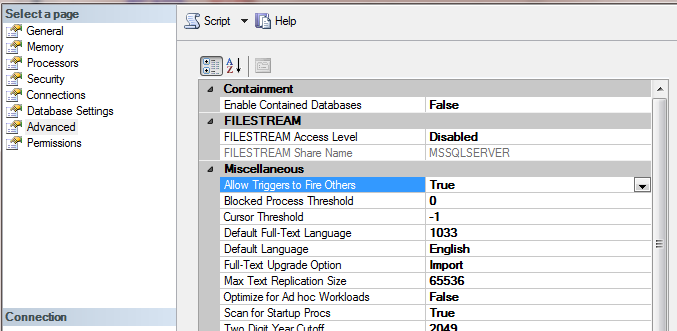
\includegraphics[width=0.75\linewidth,height=\textheight,keepaspectratio]{./images/img-019-013.png}

\begin{itemize}
\tightlist
\item
  \textbf{AFTER:} a megadott SQL utasítás sikeres végrehajtása
  \emph{után} aktiválódik. Ez azt jelenti, hogy az összes esetleges
  ellenőrző (CHECK) megszorítás, más megszorítás, valamint a DML
  utasításhoz kapcsolódó kaszkádos frissítés/törlés sikeresen lefutott.
  Ugyanazon objektumra több trigger is elhelyezhető, akár azonos típusú
  is --- például két INSERT trigger. Ebben az esetben a végrehajtási
  sorrend a trigger tulajdonságainak beállításával befolyásolható.
\item
  \textbf{INSTEAD OF:} a DML utasítás egyáltalán nem hajtódik végre,
  csak a trigger.
\end{itemize}

A DML utasítás által módosított rekordok speciális virtuális táblákon
keresztül érhetők el a trigger kódjából. Az SQL Server a következő két
virtuális táblát biztosítja:

\begin{itemize}
\tightlist
\item
  \textbf{\texttt{deleted}:} DELETE trigger esetén a törölt rekordokat,
  UPDATE trigger esetén az \emph{eredeti} (régi) rekordokat tartalmazza.
  Az UPDATE logikailag egy törlés és egy beszúrás sorozataként
  értelmezhető. INSERT trigger esetén a \texttt{deleted} tábla üres.
\item
  \textbf{\texttt{inserted}:} INSERT utasítással beszúrt rekordokat,
  illetve UPDATE trigger esetén az \emph{új} rekordokat tartalmazza.
  DELETE trigger esetén az \texttt{inserted} tábla üres.
\end{itemize}

Az SQL Server az INSERT vagy UPDATE triggerekben elérhető
\textbf{\texttt{update}}\texttt{(mezőnév)} függvényt is támogatja, amely
\texttt{true} értéket ad vissza, ha a DML utasítás módosította a
megadott mezőt. A mező nem lehet számított oszlop.

Ha a trigger hibát dob, a DML utasítás visszagörgetődik (ROLLBACK).

Egy trigger olyan kódot is futtathat, amely más triggereket vagy akár
önmagát hívja meg rekurzív módon, MS SQL Serveren legfeljebb 32 szintig.
Ezt a funkciót a szerver \texttt{nested\ triggers} (egymásba ágyazott
triggerek) beállítása szabályozza.

\subsubsection{Mikor ajánlott DML triggert
alkalmazni?}\label{mikor-ajuxe1nlott-dml-triggert-alkalmazni}

\begin{itemize}
\tightlist
\item
  \textbf{Adminisztrációs célok:} napló vezetése, vagy a módosított
  rekordok régi értékeinek megőrzése archív (történeti) táblákban.
\item
  \textbf{Adatintegritási szabályok érvényesítése}, amelyek az üzleti
  logikából következnek, és meghaladják az egyszerű elsődleges kulcs-,
  idegen kulcs- vagy CHECK-megszorítások hatókörét. Példa a Northwind
  adatbázisban:

  \begin{itemize}
  \tightlist
  \item
    Nem küldünk nehéz csomagokat külföldre. Ezért visszautasítjuk azokat
    a rendeléseket, amelyeknél a csomag tömege meghaladja a 200 kg-ot,
    és a ShipCountry nem USA. Ez megvalósítható egy INSERT AFTER vagy
    INSERT INSTEAD OF triggerrel az Orders táblán. Az ilyen
    ellenőrzéseket természetesen az ügyfélalkalmazásba is be kell
    építeni, azonban az adatbázisszintű integritásvédelem megelőzheti az
    alkalmazáshibákat vagy a hackelést.
  \end{itemize}
\item
  \textbf{Üzleti munkafolyamatok automatizálása.} Példák a Northwind
  adatbázisban:

  \begin{itemize}
  \tightlist
  \item
    Automatikus e-mail küldése a vevőnek, amikor a szállítás dátuma
    meghatározásra kerül, azaz amikor egy rendelés ShippedDate mezője
    beállításra kerül (UPDATE trigger).
  \item
    Automatikus megrendelés küldése a nagykereskedelmi szállítónak,
    amikor egy termék UnitsInStock értéke a ReorderLevel alá esik
    (UPDATE vagy INSERT trigger).
  \item
    A Products tábla UnitsInStock mezőjének automatikus frissítése,
    amikor egy kapcsolódó Order Details rekord quantity mezője
    megváltozik (UPDATE trigger).
  \end{itemize}
\end{itemize}

\textbf{GYAKORLAT:} Írj UPDATE triggert az Order Details táblára! Amikor
a mennyiség megváltozik, frissítsd a termék UnitsInStock értékét!
Feltételezheted, hogy egyszerre csak egy Order Details rekord frissül.

\textbf{GYAKORLAT:} Feltételezd, hogy a fenti feladatban egyszerre több
Order Details rekord is frissülhet!

\begin{quote}
\textbf{FIGYELMEZTETÉS:} A triggerek „csendben'' működnek, és komoly
problémák adódhatnak, ha megfeledkeznek róluk. Például ha a
rendszergazda az Order Items táblákat egy biztonsági másolatból egy
UPDATE utasítással állítja vissza anélkül, hogy először letiltaná a
triggert\ldots{}
\end{quote}

További példák SQL Server triggerekre:
http://sqlhints.com/2016/02/28/inserted-and-deleted-logical-tables-in-sql-server/

\begin{center}\rule{0.5\linewidth}{0.5pt}\end{center}

\subsection{Szoros csatolás}\label{szoros-csatoluxe1s}

Az alábbi példában egy olyan új INSERT triggert hozunk létre az Orders
táblán, amely sokáig fut és kivételt dob --- ezzel megbénítja a
rendelésmentési folyamatot.

\begin{Shaded}
\begin{Highlighting}[]
\KeywordTok{drop} \KeywordTok{trigger}\NormalTok{ tr\_demo\_bad}
\NormalTok{go}
\KeywordTok{create} \KeywordTok{trigger}\NormalTok{ tr\_demo\_bad }\KeywordTok{on}\NormalTok{ orders }\ControlFlowTok{for} \KeywordTok{insert} \KeywordTok{as}
\KeywordTok{declare}\NormalTok{ @orderid }\DataTypeTok{int}
\KeywordTok{select}\NormalTok{ @orderid}\OperatorTok{=}\NormalTok{OrderID }\KeywordTok{from}\NormalTok{ inserted}
\NormalTok{print }\StringTok{\textquotesingle{}New order ID: \textquotesingle{}} \OperatorTok{+} \FunctionTok{cast}\NormalTok{(@orderid }\KeywordTok{as} \DataTypeTok{varchar}\NormalTok{(}\DecValTok{50}\NormalTok{))}
\NormalTok{waitfor delay }\StringTok{\textquotesingle{}00:00:10\textquotesingle{}}  \CommentTok{{-}{-}10 s}
\KeywordTok{select} \DecValTok{1}\OperatorTok{/}\DecValTok{0}  \CommentTok{{-}{-}hibát generálunk}
\NormalTok{go}
\CommentTok{{-}{-}1. teszt: az utolsó két sorral kikommentezve}
\KeywordTok{insert}\NormalTok{ Orders (CustomerID, OrderDate) }\KeywordTok{values}\NormalTok{ (}\StringTok{\textquotesingle{}AROUT\textquotesingle{}}\NormalTok{, GETDATE())}
\CommentTok{{-}{-}tábla visszaállítása}
\KeywordTok{delete}\NormalTok{ Orders }\KeywordTok{where}\NormalTok{ CustomerID}\OperatorTok{=}\StringTok{\textquotesingle{}AROUT\textquotesingle{}} \KeywordTok{and}\NormalTok{ EmployeeID }\KeywordTok{is} \KeywordTok{null}
\CommentTok{{-}{-}2. teszt: a trigger újbóli létrehozása, az utolsó sorokkal kikommentezve}
\KeywordTok{insert}\NormalTok{ Orders (CustomerID, OrderDate) }\KeywordTok{values}\NormalTok{ (}\StringTok{\textquotesingle{}AROUT\textquotesingle{}}\NormalTok{, GETDATE())}
\CommentTok{{-}{-}sokáig kell várnunk, de nincs hiba}
\CommentTok{{-}{-}3. teszt: a trigger újbóli létrehozása, minden sorral}
\KeywordTok{insert}\NormalTok{ Orders (CustomerID, OrderDate) }\KeywordTok{values}\NormalTok{ (}\StringTok{\textquotesingle{}AROUT\textquotesingle{}}\NormalTok{, GETDATE())}
\CommentTok{{-}{-}sokáig kell várnunk, majd megkapjuk az üzenetet:}
\CommentTok{{-}{-} \textquotesingle{}New order ID: 11094}
\CommentTok{{-}{-} Msg 8134, Level 16, State 1, Procedure tr\_demo\_bad, Line 6 [...]}
\CommentTok{{-}{-} Divide by zero error encountered. The statement has been terminated.\textquotesingle{}}
\KeywordTok{select} \OperatorTok{*} \KeywordTok{from}\NormalTok{ Orders }\KeywordTok{where}\NormalTok{ CustomerID}\OperatorTok{=}\StringTok{\textquotesingle{}AROUT\textquotesingle{}} \KeywordTok{and}\NormalTok{ EmployeeID }\KeywordTok{is} \KeywordTok{null}
\CommentTok{{-}{-}nincs ilyen rekord, mert}
\CommentTok{{-}{-}az insert utasítás visszagörgetésre került {-}\textgreater{} a kereskedelmi rendszer működése megszakadt}
\end{Highlighting}
\end{Shaded}

Ez pontosan az, amit el kell kerülnünk. A \emph{szoros csatolás} helyett
\emph{laza csatolást} valósítunk meg.

\begin{center}\rule{0.5\linewidth}{0.5pt}\end{center}

\subsection{A lazán csatolt rendszer}\label{a-lazuxe1n-csatolt-rendszer}

Az alapötlet: a trigger csak az eseményeket menti egy naplótáblába. A
táblát ezután egy tárolt eljárás dolgozza fel.

\subsubsection{A naplótábla és a
trigger}\label{a-napluxf3tuxe1bla-uxe9s-a-trigger}

A trigger az \texttt{inserted} és \texttt{deleted} virtuális táblákat
használja. Ez a trigger több rekordot érintő INSERT és UPDATE
műveleteket is kezelni tud.

\begin{Shaded}
\begin{Highlighting}[]
\CommentTok{{-}{-}a naplótábla}
\NormalTok{go}
\CommentTok{{-}{-}drop table order\_log}
\NormalTok{go}
\KeywordTok{create} \KeywordTok{table}\NormalTok{ order\_log (}
\NormalTok{    event\_id }\DataTypeTok{int}\NormalTok{ IDENTITY (}\DecValTok{1}\NormalTok{, }\DecValTok{1}\NormalTok{) }\KeywordTok{primary} \KeywordTok{key}\NormalTok{ ,}
\NormalTok{    event\_type }\DataTypeTok{varchar}\NormalTok{(}\DecValTok{50}\NormalTok{) }\KeywordTok{NOT} \KeywordTok{NULL}\NormalTok{ ,}
\NormalTok{    order\_id }\DataTypeTok{int} \KeywordTok{NOT} \KeywordTok{NULL}\NormalTok{ ,}
\NormalTok{    orderitem\_id }\DataTypeTok{int} \KeywordTok{NULL}\NormalTok{ ,}
\NormalTok{    status }\DataTypeTok{int} \KeywordTok{NOT} \KeywordTok{NULL} \KeywordTok{default}\NormalTok{(}\DecValTok{0}\NormalTok{),}
\NormalTok{    time\_created datetime }\KeywordTok{NOT} \KeywordTok{NULL} \KeywordTok{default}\NormalTok{(getdate()) ,}
\NormalTok{    time\_process\_begin datetime }\KeywordTok{NULL}\NormalTok{ ,}
\NormalTok{    time\_process\_end datetime }\KeywordTok{NULL}\NormalTok{ ,}
\NormalTok{    process\_duration }\KeywordTok{as}\NormalTok{ datediff(}\DataTypeTok{second}\NormalTok{, time\_process\_begin, time\_process\_end)}
\NormalTok{)}
\NormalTok{go}
\KeywordTok{drop} \KeywordTok{trigger}\NormalTok{ tr\_log\_order}
\NormalTok{go}
\KeywordTok{create} \KeywordTok{trigger}\NormalTok{ tr\_log\_order }\KeywordTok{ON}\NormalTok{ Orders }\ControlFlowTok{for} \KeywordTok{insert}\NormalTok{, }\KeywordTok{update} \KeywordTok{as}
\KeywordTok{declare}\NormalTok{ @orderid }\DataTypeTok{int}
\KeywordTok{select}\NormalTok{ @orderid}\OperatorTok{=}\NormalTok{orderid }\KeywordTok{from}\NormalTok{ inserted  }\CommentTok{{-}{-}FIGYELEM: ha több rekord szerepel az inserted táblában, csak az utolsó értékét kapjuk meg — ez hibás működéshez vezethet}
\NormalTok{print }\StringTok{\textquotesingle{}OrderID of the LAST record: \textquotesingle{}} \OperatorTok{+} \FunctionTok{cast}\NormalTok{(@orderid }\KeywordTok{as} \DataTypeTok{varchar}\NormalTok{(}\DecValTok{50}\NormalTok{))}
\ControlFlowTok{if} \KeywordTok{update}\NormalTok{(orderid) }\ControlFlowTok{begin}  \CommentTok{{-}{-}ha az orderid megváltozott, akkor ez egy INSERT}
\NormalTok{    print }\StringTok{\textquotesingle{}Warning: new order\textquotesingle{}}
    \KeywordTok{insert}\NormalTok{ order\_log (event\_type, order\_id)  }\CommentTok{{-}{-}a status és time\_created az alapértelmezett értéket kapja}
        \KeywordTok{select} \StringTok{\textquotesingle{}new order\textquotesingle{}}\NormalTok{, orderid }\KeywordTok{from}\NormalTok{ inserted}
\ControlFlowTok{end} \ControlFlowTok{else} \ControlFlowTok{if} \KeywordTok{update}\NormalTok{(shipaddress) }\KeywordTok{or} \KeywordTok{update}\NormalTok{(shipcity) }\ControlFlowTok{begin}  \CommentTok{{-}{-}a szállítási cím megváltozott}
\NormalTok{    print }\StringTok{\textquotesingle{}Warning: address changed\textquotesingle{}}
    \KeywordTok{insert}\NormalTok{ order\_log (event\_type, order\_id)}
        \KeywordTok{select} \StringTok{\textquotesingle{}address changed\textquotesingle{}}\NormalTok{, orderid }\KeywordTok{from}\NormalTok{ inserted}
\ControlFlowTok{end} \ControlFlowTok{else} \ControlFlowTok{begin}  \CommentTok{{-}{-}egyéb változás}
\NormalTok{    print }\StringTok{\textquotesingle{}Warning: other change\textquotesingle{}}
    \KeywordTok{insert}\NormalTok{ order\_log (event\_type, order\_id)}
        \KeywordTok{select} \StringTok{\textquotesingle{}other change\textquotesingle{}}\NormalTok{, orderid }\KeywordTok{from}\NormalTok{ inserted}
\ControlFlowTok{end}
\NormalTok{go}

\CommentTok{{-}{-}1. teszt}
\KeywordTok{insert}\NormalTok{ Orders (CustomerID, OrderDate) }\KeywordTok{values}\NormalTok{ (}\StringTok{\textquotesingle{}AROUT\textquotesingle{}}\NormalTok{, GETDATE())}
\KeywordTok{select} \OperatorTok{*} \KeywordTok{from}\NormalTok{ order\_log}
\CommentTok{{-}{-}egy új rekordot kaptunk a naplótáblában}

\CommentTok{{-}{-}2. teszt}
\KeywordTok{insert}\NormalTok{ Orders (CustomerID, OrderDate) }\KeywordTok{values}\NormalTok{ (}\StringTok{\textquotesingle{}AROUT\textquotesingle{}}\NormalTok{, GETDATE()), (}\StringTok{\textquotesingle{}HANAR\textquotesingle{}}\NormalTok{, GETDATE())}
\KeywordTok{select} \OperatorTok{*} \KeywordTok{from}\NormalTok{ order\_log}
\CommentTok{{-}{-}két új rekordot kaptunk a naplótáblában}

\CommentTok{{-}{-}3. teszt}
\KeywordTok{update}\NormalTok{ Orders }\KeywordTok{set}\NormalTok{ ShipVia }\OperatorTok{=} \DecValTok{3} \KeywordTok{where}\NormalTok{ OrderID }\KeywordTok{in}\NormalTok{ (}\DecValTok{11097}\NormalTok{, }\DecValTok{11096}\NormalTok{)  }\CommentTok{{-}{-}a 2. teszt rendelésazonosítói}
\KeywordTok{select} \OperatorTok{*} \KeywordTok{from}\NormalTok{ order\_log}
\CommentTok{{-}{-}két új \textquotesingle{}other change\textquotesingle{} típusú rekordot kaptunk}

\CommentTok{{-}{-}táblák visszaállítása}
\KeywordTok{delete}\NormalTok{ Orders }\KeywordTok{where}\NormalTok{ CustomerID }\KeywordTok{in}\NormalTok{ (}\StringTok{\textquotesingle{}AROUT\textquotesingle{}}\NormalTok{, }\StringTok{\textquotesingle{}HANAR\textquotesingle{}}\NormalTok{) }\KeywordTok{and}\NormalTok{ EmployeeID }\KeywordTok{is} \KeywordTok{null}
\KeywordTok{delete}\NormalTok{ order\_log}
\end{Highlighting}
\end{Shaded}

\subsubsection{A tárolt eljárás az új rendelések
feldolgozásához}\label{a-tuxe1rolt-eljuxe1ruxe1s-az-uxfaj-rendeluxe9sek-feldolgozuxe1suxe1hoz}

Tegyük fel, hogy az új rendelés tételeinek rögzítése a rendelési rekord
létrehozása után következik.

\begin{Shaded}
\begin{Highlighting}[]
\CommentTok{{-}{-}egyszerű tárolt eljárás, amely feldolgoz egy új rendelést}
\CommentTok{{-}{-}és 0{-}t ad vissza, ha az összes tétel hibamentesen rögzíthető a készletbe}
\CommentTok{{-}{-}egyben bemutatja az OUTPUT paraméterek használatát}
\KeywordTok{drop}\NormalTok{ proc sp\_commit\_new\_order\_to\_inventory}
\NormalTok{go}
\KeywordTok{create} \KeywordTok{procedure}\NormalTok{ sp\_commit\_new\_order\_to\_inventory}
\OtherTok{@orderid int,}
\OtherTok{@result int output}
\KeywordTok{as}
\ControlFlowTok{begin}\NormalTok{ try}
    \KeywordTok{update}\NormalTok{ products }\KeywordTok{set}\NormalTok{ unitsInStock }\OperatorTok{=}\NormalTok{ unitsInStock }\OperatorTok{{-}}\NormalTok{ od.quantity}
    \KeywordTok{from}\NormalTok{ products p }\KeywordTok{inner} \KeywordTok{join}\NormalTok{ [}\KeywordTok{Order}\NormalTok{ Details] od }\KeywordTok{on}\NormalTok{ od.ProductID}\OperatorTok{=}\NormalTok{p.ProductID}
    \KeywordTok{where}\NormalTok{ od.OrderID}\OperatorTok{=}\NormalTok{@orderid}
    \KeywordTok{set}\NormalTok{ @result}\OperatorTok{=}\DecValTok{0}
\ControlFlowTok{end}\NormalTok{ try}
\ControlFlowTok{begin}\NormalTok{ catch}
\NormalTok{    print }\StringTok{\textquotesingle{} Inventory error: \textquotesingle{}}\OperatorTok{+}\NormalTok{ ERROR\_MESSAGE() }\OperatorTok{+} \StringTok{\textquotesingle{} (\textquotesingle{}} \OperatorTok{+} \FunctionTok{cast}\NormalTok{(ERROR\_NUMBER() }\KeywordTok{as} \DataTypeTok{varchar}\NormalTok{(}\DecValTok{20}\NormalTok{)) }\OperatorTok{+} \StringTok{\textquotesingle{})\textquotesingle{}}
    \KeywordTok{set}\NormalTok{ @result}\OperatorTok{=}\DecValTok{1}
\ControlFlowTok{end}\NormalTok{ catch}
\NormalTok{go}

\CommentTok{{-}{-}teszt}
\KeywordTok{select} \OperatorTok{*} \KeywordTok{from}\NormalTok{ order\_log  }\CommentTok{{-}{-}11097}
\KeywordTok{select} \OperatorTok{*} \KeywordTok{from}\NormalTok{ Products }\KeywordTok{where}\NormalTok{ ProductID}\OperatorTok{=}\DecValTok{10}  \CommentTok{{-}{-}unitsinstock =31}
\KeywordTok{select} \OperatorTok{*} \KeywordTok{from}\NormalTok{ Products }\KeywordTok{where}\NormalTok{ ProductID}\OperatorTok{=}\DecValTok{9}   \CommentTok{{-}{-}unitsinstock =29}
\KeywordTok{insert}\NormalTok{ [}\KeywordTok{Order}\NormalTok{ Details] (orderid, productid, quantity, UnitPrice, Discount)}
\KeywordTok{values}\NormalTok{ (}\DecValTok{11097}\NormalTok{, }\DecValTok{9}\NormalTok{, }\DecValTok{10}\NormalTok{, }\DecValTok{30}\NormalTok{, }\DecValTok{0}\NormalTok{),(}\DecValTok{11097}\NormalTok{, }\DecValTok{10}\NormalTok{, }\DecValTok{40}\NormalTok{, }\DecValTok{30}\NormalTok{, }\DecValTok{0}\NormalTok{)  }\CommentTok{{-}{-}a második tétel hibát fog okozni}
\NormalTok{go}
\KeywordTok{declare}\NormalTok{ @res }\DataTypeTok{int}
\KeywordTok{exec}\NormalTok{ sp\_commit\_new\_order\_to\_inventory }\DecValTok{11097}\NormalTok{, @res output}
\NormalTok{print @res}
\KeywordTok{exec}\NormalTok{ sp\_commit\_new\_order\_to\_inventory }\DecValTok{11096}\NormalTok{, @res output}
\NormalTok{print @res}
\NormalTok{go}
\CommentTok{{-}{-}ellenőrzés: az unitsinstock értéke nem változott (OK)}
\KeywordTok{select} \OperatorTok{*} \KeywordTok{from}\NormalTok{ Products }\KeywordTok{where}\NormalTok{ ProductID}\OperatorTok{=}\DecValTok{10}  \CommentTok{{-}{-}unitsinstock =31}
\KeywordTok{select} \OperatorTok{*} \KeywordTok{from}\NormalTok{ Products }\KeywordTok{where}\NormalTok{ ProductID}\OperatorTok{=}\DecValTok{9}   \CommentTok{{-}{-}unitsinstock =29}
\end{Highlighting}
\end{Shaded}

\subsubsection{A tárolt eljárás az eseménynapló
feldolgozásához}\label{a-tuxe1rolt-eljuxe1ruxe1s-az-esemuxe9nynapluxf3-feldolgozuxe1suxe1hoz}

Mivel az esemény típusától függően teljesen eltérő műveleteket kell
elvégezni, kurzorral iterálunk az eseménynapló rekordjain.

\begin{Shaded}
\begin{Highlighting}[]
\CommentTok{{-}{-}tárolt eljárás az order\_log feldolgozásához}
\CommentTok{{-}{-}drop proc sp\_order\_process}
\NormalTok{go}
\KeywordTok{create}\NormalTok{ proc sp\_order\_process }\KeywordTok{as}
\KeywordTok{declare}\NormalTok{ @event\_id }\DataTypeTok{int}\NormalTok{, @event\_type }\DataTypeTok{varchar}\NormalTok{(}\DecValTok{50}\NormalTok{), @order\_id }\DataTypeTok{int}\NormalTok{, @result }\DataTypeTok{int}
\KeywordTok{declare}\NormalTok{ cursor\_events }\KeywordTok{cursor}\NormalTok{ forward\_only }\KeywordTok{static}
    \ControlFlowTok{for}
    \KeywordTok{select}\NormalTok{  event\_id, event\_type, order\_id}
    \KeywordTok{from}\NormalTok{ order\_log }\KeywordTok{where}\NormalTok{ status}\OperatorTok{=}\DecValTok{0}  \CommentTok{{-}{-}csak a feldolgozatlan eseményeket kezeljük}

\KeywordTok{set}\NormalTok{ xact\_abort }\KeywordTok{on}
\KeywordTok{set}\NormalTok{ nocount }\KeywordTok{on}
\KeywordTok{open}\NormalTok{ cursor\_events}
\NormalTok{fetch }\KeywordTok{next} \KeywordTok{from}\NormalTok{ cursor\_events }\KeywordTok{into}\NormalTok{ @event\_id, @event\_type, @order\_id}
\ControlFlowTok{while}\NormalTok{ @@fetch\_status }\OperatorTok{=} \DecValTok{0}
\ControlFlowTok{begin}
\NormalTok{    print }\StringTok{\textquotesingle{}Processing event ID=\textquotesingle{}} \OperatorTok{+} \FunctionTok{cast}\NormalTok{(@event\_id }\KeywordTok{as} \DataTypeTok{varchar}\NormalTok{(}\DecValTok{10}\NormalTok{)) }\OperatorTok{+} \StringTok{\textquotesingle{}, Order ID=\textquotesingle{}} \OperatorTok{+}
\FunctionTok{cast}\NormalTok{(@order\_id }\KeywordTok{as} \DataTypeTok{varchar}\NormalTok{(}\DecValTok{10}\NormalTok{))}
    \KeywordTok{update}\NormalTok{ order\_log }\KeywordTok{set}\NormalTok{ time\_process\_begin}\OperatorTok{=}\NormalTok{getdate() }\KeywordTok{where}\NormalTok{ event\_id}\OperatorTok{=}\NormalTok{@event\_id}
    \ControlFlowTok{begin}\NormalTok{ tran}
    \KeywordTok{set}\NormalTok{ @result }\OperatorTok{=} \KeywordTok{null}
    \ControlFlowTok{if}\NormalTok{ @event\_type }\OperatorTok{=} \StringTok{\textquotesingle{}new order\textquotesingle{}} \ControlFlowTok{begin}
\NormalTok{        print }\StringTok{\textquotesingle{}  Processing new order...\textquotesingle{}}
        \KeywordTok{exec}\NormalTok{ sp\_commit\_new\_order\_to\_inventory @order\_id, @result output}
    \ControlFlowTok{end} \ControlFlowTok{else} \ControlFlowTok{if}\NormalTok{ @event\_type }\OperatorTok{=} \StringTok{\textquotesingle{}address changed\textquotesingle{}} \ControlFlowTok{begin}
\NormalTok{        print }\StringTok{\textquotesingle{}  Processing address changed...\textquotesingle{}}
\NormalTok{        waitfor delay }\StringTok{\textquotesingle{}00:00:01\textquotesingle{}}  \CommentTok{{-}{-}csak szimuláljuk a többi eseménytípus feldolgozását}
        \KeywordTok{set}\NormalTok{ @result}\OperatorTok{=}\DecValTok{0}
    \ControlFlowTok{end} \ControlFlowTok{else} \ControlFlowTok{if}\NormalTok{ @event\_type }\OperatorTok{=} \StringTok{\textquotesingle{}other change\textquotesingle{}} \ControlFlowTok{begin}
\NormalTok{        print }\StringTok{\textquotesingle{}  Processing other change...\textquotesingle{}}
\NormalTok{        waitfor delay }\StringTok{\textquotesingle{}00:00:01\textquotesingle{}}
        \KeywordTok{set}\NormalTok{ @result}\OperatorTok{=}\DecValTok{0}
    \ControlFlowTok{end} \ControlFlowTok{else} \ControlFlowTok{begin}
\NormalTok{        print }\StringTok{\textquotesingle{}  Unknown event type...\textquotesingle{}}
\NormalTok{        waitfor delay }\StringTok{\textquotesingle{}00:00:01\textquotesingle{}}
        \KeywordTok{set}\NormalTok{ @result}\OperatorTok{=}\DecValTok{1}
    \ControlFlowTok{end}

    \ControlFlowTok{if}\NormalTok{ @result}\OperatorTok{=}\DecValTok{0} \ControlFlowTok{begin}
\NormalTok{        print }\StringTok{\textquotesingle{}Event processing OK\textquotesingle{}}
        \KeywordTok{commit}\NormalTok{ tran}
    \ControlFlowTok{end} \ControlFlowTok{else} \ControlFlowTok{begin}
\NormalTok{        print }\StringTok{\textquotesingle{}Event processing failed\textquotesingle{}}
        \KeywordTok{rollback}\NormalTok{ tran}
    \ControlFlowTok{end}
\NormalTok{    print }\StringTok{\textquotesingle{}\textquotesingle{}}
    \KeywordTok{update}\NormalTok{ order\_log }\KeywordTok{set}\NormalTok{ time\_process\_end}\OperatorTok{=}\NormalTok{getdate(),}
\NormalTok{        status}\OperatorTok{=}\ControlFlowTok{case} \ControlFlowTok{when}\NormalTok{ @result}\OperatorTok{=}\DecValTok{0} \ControlFlowTok{then} \DecValTok{2} \ControlFlowTok{else} \DecValTok{1} \ControlFlowTok{end}
        \KeywordTok{where}\NormalTok{ event\_id}\OperatorTok{=}\NormalTok{@event\_id}
\NormalTok{    fetch }\KeywordTok{next} \KeywordTok{from}\NormalTok{ cursor\_events }\KeywordTok{into}\NormalTok{ @event\_id, @event\_type, @order\_id}
\ControlFlowTok{end}
\KeywordTok{close}\NormalTok{ cursor\_events }\KeywordTok{deallocate}\NormalTok{ cursor\_events}
\NormalTok{go}

\CommentTok{{-}{-}teszt}
\KeywordTok{update}\NormalTok{ order\_log }\KeywordTok{set}\NormalTok{ status}\OperatorTok{=}\DecValTok{0}
\KeywordTok{select} \OperatorTok{*}\KeywordTok{from}\NormalTok{ orders }\KeywordTok{where}\NormalTok{ EmployeeID }\KeywordTok{is} \KeywordTok{null}
\KeywordTok{select} \OperatorTok{*} \KeywordTok{from}\NormalTok{ order\_log}
\KeywordTok{exec}\NormalTok{ dbo.sp\_order\_process}
\KeywordTok{select} \OperatorTok{*} \KeywordTok{from}\NormalTok{ order\_log}
\end{Highlighting}
\end{Shaded}

\textbf{Várható kimenet:}

\begin{verbatim}
Processing event ID=5, Order ID=11097
 Processing new order...
 Inventory error: The UPDATE statement conflicted with the CHECK constraint etc.
Event processing failed

Processing event ID=6, Order ID=11096
 Processing new order...
Event processing OK
\end{verbatim}

\subsubsection{Az eseménynaplót feldolgozó ütemezett
feladat}\label{az-esemuxe9nynapluxf3t-feldolgozuxf3-uxfctemezett-feladat}

Az ütemezett feladatot (job) az SSMS grafikus felületével valósítjuk
meg, és a Job Activity Monitor segítségével ellenőrizzük a működését.

\begin{center}\rule{0.5\linewidth}{0.5pt}\end{center}

\textbf{GYAKORLAT:} Hozz létre egy lazán csatolt megoldást, amely
figyeli a Products táblát, és új készletutánpótlást rendel a kapcsolódó
Supplier-től (Szállítótól), amikor az \texttt{UnitsInStock} értéke a
\texttt{ReorderLevel} mezőben meghatározott érték alá esik!

\section{3. Replikáció, naplószállítás és
feladatátvétel}\label{replikuxe1ciuxf3-napluxf3szuxe1lluxedtuxe1s-uxe9s-feladatuxe1tvuxe9tel}

A laza csatolásos esettanulmányban valójában a \emph{replikáció} egy
speciális formáját valósítottuk meg.

\subsection{Replikációs fogalmak és
architektúra}\label{replikuxe1ciuxf3s-fogalmak-uxe9s-architektuxfara}

A \emph{replika} az eredeti másolatát jelenti. Az
adatbázis-technológiában a replikációt arra használják, hogy egy vagy
több forrásból automatikusan másolják és szinkronizálják az adatokat. A
replikációs metafora összetevői a következők:

\begin{itemize}
\tightlist
\item
  A \textbf{közzétevő} (publisher) az az entitás (adatbázis-szerver),
  amelynek adatait meg kell osztani. Az adatok \textbf{kiadványokba}
  (publications) vannak szervezve. Minden kiadvány egy vagy több
  \textbf{cikket} (articles) tartalmaz. A cikkek lehetnek táblák,
  táblarészletek, tárolt eljárások vagy más adatbázis-objektumok.
\end{itemize}

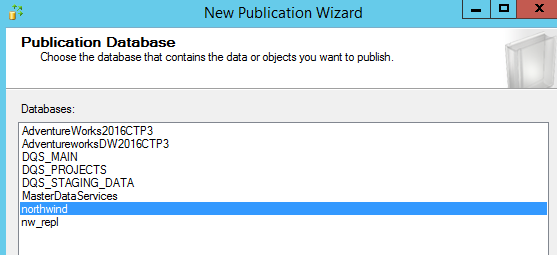
\includegraphics[width=0.75\linewidth,height=\textheight,keepaspectratio]{./images/img-027-015.png}

\begin{itemize}
\item
  Az \textbf{előfizető} (subscriber) az az entitás, amely feliratkozik a
  kiadványokra. Lehet ugyanaz az adatbázis-szerver, mint a közzétevő,
  vagy egy másik szerver. Több előfizető --- esetleg különböző
  szervereken --- is feliratkozhat ugyanarra a kiadványra.
\item
  A \textbf{feliratkozásnak} (subscription) különböző módozatai lehetnek
  a másolás módjával és ütemezésével kapcsolatban. Tartalmazhat
  adatszűrőket vagy menet közbeni adatátalakítási lépéseket. Lehet
  \textbf{push} (tolt, azaz a közzétevő indítja) vagy \textbf{pull}
  (húzott, azaz az előfizető indítja) feliratkozás. A pull
  feliratkozásokat az előfizető hozza létre és ütemezi.
\end{itemize}

A replikáció fő típusai és alkalmazási esetei a következők:

\begin{itemize}
\tightlist
\item
  \textbf{Pillanatkép-replikáció} (Snapshot replication). A cikkek
  kezdeti pillanatfelvétele után a másolt objektumokat az előfizetőnél
  minden adatfrissítéskor töröljük és újra létrehozzuk --- függetlenül
  attól, hogy volt-e változás a kiadványban. Akkor alkalmazható, ha egy
  OLTP adatbázis részeit másolni kell egy adattárházba vagy egy
  riportszerverbe, munkaidőn kívüli ütemezéssel. Példa: a nap folyamán
  keletkezett adatok éjszakai küldése (`adott időpontra vonatkozó
  riportok'). Mivel több feliratkozás is mutathat ugyanarra a
  céladatbázisra, a replikáció ETL (extract--transform--load, azaz
  kinyerés--átalakítás--betöltés) mechanizmusként is használható, ha az
  összes közzétevő SQL Server technológiát alkalmaz. \textbf{FIGYELEM:}
  a törlés/újralétrehozás mechanizmusa miatt az előfizetőnél lévő
  objektumok ideiglenesen nem lesznek elérhetők, ami rövid
  szolgáltatáskimaradást okozhat. Az adatok késleltetését is el kell
  viselni. \emph{Minden más alábbi replikációs típust
  pillanatfelvétellel inicializálnak.}
\end{itemize}

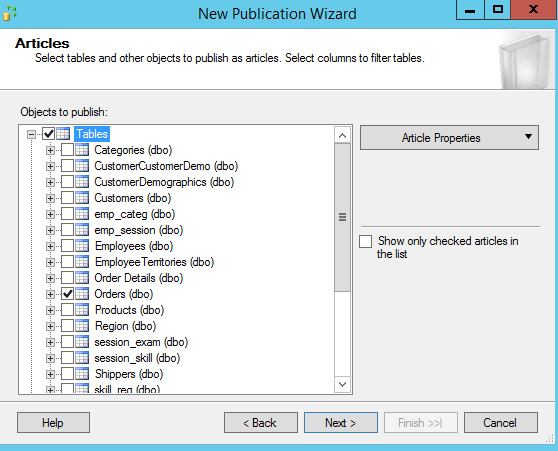
\includegraphics[width=0.75\linewidth,height=\textheight,keepaspectratio]{./images/img-028-016.png}

\begin{itemize}
\item
  \textbf{Tranzakciós replikáció} (Transactional replication). Csak a
  megváltozott adatokat másolja, és közel valós idejű
  adatszinkronizációra konfigurálható. Szükség van elsődleges kulcsra a
  replikált táblákon. Akkor alkalmazható, ha a nagy késleltetés
  problémát jelent, és nem akarjuk a változatlan adatokat is mozgatni.
  Példa: egy vállalat külső telephelyei saját helyi szerverekkel
  rendelkeznek, amelyek a központi adatbázis csak a működésükhöz
  szükséges részeit tárolják. Ez az architektúra javítja a helyszíni
  autonómiát és az információs rendszer megbízhatóságát.
\item
  \textbf{Összefésülő replikáció} (Merge replication). Ebben a sémában
  az előfizetők maguk is módosíthatják az adatokat, és egy mechanizmus
  gondoskodik arról, hogy ezek a változások minden félhez eljussanak, és
  konzisztens adatbázissá olvadjanak össze. Az összefésülési folyamat
  konfliktusfeloldást is magában foglalhat. A rekordok több szerveren
  keresztüli azonosítása érdekében a tábláknak UNIQUEIDENTIFIER típusú,
  ROWGUIDCOL tulajdonságú mezővel kell rendelkezniük.\footnote{Úgy
    működik, mint egy identity oszlop, de kezdőérték nélkül és
    globálisan egyedi értékekkel. Használat:
    \texttt{CREATE\ TABLE\ test\ (my\_guid\ uniqueidentifier\ DEFAULT\ NEWSEQUENTIALID()\ ROWGUIDCOL,\ …)}}
  Tipikus eset az utazó üzletkötők esete, akik nem folyamatosan
  kapcsolódnak a központi adatbázishoz. A helyi adatbázisukban végzett
  módosítások automatikusan összefésülődnek a többi módosítással.
\end{itemize}

A replikáció típusát mindig a kiadvány határozza meg.

A replikációs technológia ütemezett feladatokon alapul, összefésülő
replikáció esetén pedig a közzétett cikkek triggerein is.

A replikáció \textbf{nem ajánlott}, ha egy teljes adatbázis pontos
másolatát kell karbantartani egy távoli szerveren a rendelkezésre állás
és megbízhatóság javítása érdekében --- erre a célra a naplószállítás és
az SQL Server 2012-től elérhető Always On technológia egyszerűbb és
robusztusabb megoldást kínál.

\textbf{FIGYELEM:} bár a replikáció az adatok több példányát tartja
karban, nem helyettesíti a biztonsági mentést és a katasztrófa utáni
helyreállítás tervezését.

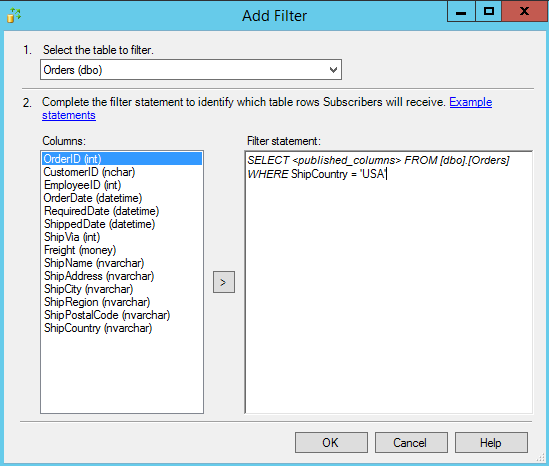
\includegraphics[width=0.75\linewidth,height=\textheight,keepaspectratio]{./images/img-029-017.png}

A replikációban három \textbf{szerverszerepkör} van: a \emph{közzétevő},
a \emph{terjesztő} (distributor) és az \emph{előfizető}. Mindhárom
szerepet ugyanaz a szerverpéldány is betöltheti, ha egy helyi adatbázist
egy másik helyi adatbázisba replikálnak, vagy különböző példányok
tölthetik be őket. Reálisabb konfigurációkban a terjesztő szerepét egy
másik szerver veszi át, hogy tehermentesítse a közzétevőt. \textbf{A
terjesztő} felelős a megváltozott adatok tárolásáért egy megosztott
mappában vagy egy terjesztési adatbázisban, és az adatok továbbításáért
az előfizetőknek. Egy közzétevőhöz csak egy terjesztő tartozhat, de egy
terjesztő több előfizetőt is kiszolgálhat.

\textbf{Kétirányú} vagy \textbf{frissíthető} replikáció esetén az
előfizető is módosíthatja a közzétevőn lévő adatokat.

Az SQL Server különféle \textbf{ügynökökkel} (agents) valósítja meg a
replikációs funkcionalitást. Ezek az ügynökök az SQL Server Agent által
felügyelt feladatokként futnak.

\begin{itemize}
\tightlist
\item
  \textbf{A pillanatkép-ügynök} (Snapshot agent) előállítja a
  pillanatfelvételt, és a terjesztőnél lévő
  \textbf{pillanatfelvétel-mappában} tárolja. Az ügynök a \texttt{bcp}
  (bulk copy) segédprogramot használja a kiadvány cikkeinek másolásához.
\end{itemize}

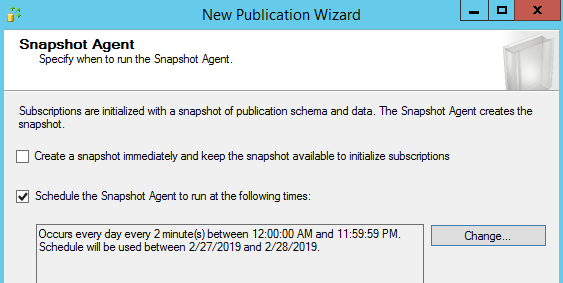
\includegraphics[width=0.75\linewidth,height=\textheight,keepaspectratio]{./images/img-029-018.png}

\begin{itemize}
\item
  \textbf{A terjesztési ügynök} (Distribution agent).
  Pillanatkép-replikációban ez az ügynök alkalmazza a pillanatfelvételt
  az előfizetőre; tranzakciós replikációban futtatja a
  \textbf{terjesztési adatbázisban} tárolt tranzakciókat az előfizetőn.
  A terjesztési adatbázis egy rendszeradatbázis a terjesztőn, ezért a
  System Databases csoportban találod meg. Ez az ügynök pull
  feliratkozásnál az előfizetőn, push feliratkozásnál a közzétevőn fut.
\item
  \textbf{A naplóolvasó ügynök} (Log reader agent) olvassa a tranzakciós
  naplót a közzétevőnél, és a releváns tranzakciókat átmásolja a
  terjesztési adatbázisba. Csak tranzakciós replikációban használják.
  Minden közzétett adatbázishoz külön ügynök tartozik.
\item
  \textbf{A sorkezelő ügynök} (Queue reader agent) az előfizetők által
  végzett módosításokat másolja a közzétevőre \emph{frissíthető} vagy
  \emph{kétirányú} tranzakciós replikáció esetén.
\item
  \textbf{Az összefésülési ügynök} (Merge agent) összefésüli az
  előfizetőnél és a közzétevőnél egyaránt keletkező növekményes
  változásokat összefésülő replikációban. A változások felismerése
  triggereken alapul. Az összefésülési ügynököt tranzakciós
  replikációban nem használják.
\end{itemize}

Pull feliratkozás kivételével az összes ügynök a terjesztőn fut.

\begin{center}\rule{0.5\linewidth}{0.5pt}\end{center}

\subsection{Pillanatkép-replikáció}\label{pillanatkuxe9p-replikuxe1ciuxf3}

Először állítsd be a tesztkörnyezetet. A replikációs példák megfelelő
működéséhez három `nevesített' MS SQL Server példányra van szükség,
amelyek ugyanazon a szervergépen vannak telepítve. Ezeket PRIM, SECOND
és THIRD névvel kell ellátni.

\textbf{Forgatókönyv:} az amerikai ügyfelek rendeléseit szeretnénk
átreplikálni ugyanazon a szerveren (Principal) lévő másik adatbázisba,
hogy éjszaka frissítsük a riportadattárházat. Pillanatkép-replikációt
választunk.

\subsubsection{A kiadvány
létrehozása}\label{a-kiadvuxe1ny-luxe9trehozuxe1sa}

\begin{enumerate}
\def\labelenumi{\arabic{enumi}.}
\item
  Csatlakozz a Principal szerverhez, és hozz létre egy új adatbázist
  Northwind névvel, ha még nem létezik. Futtasd a Northwind
  adatbázis-létrehozó szkriptjét (dump).
\item
  Az alábbi hiba elkerülése érdekében: \emph{„Cannot execute as the
  database principal because the principal ``dbo'' does not exist,
  \ldots``} --- amely a Northwind adatbázis hiányos visszaállításából
  ered --- futtasd a következő szkriptet a Northwind adatbázison:
\end{enumerate}

\begin{Shaded}
\begin{Highlighting}[]
\KeywordTok{EXEC}\NormalTok{ sp\_changedbowner }\StringTok{\textquotesingle{}sa\textquotesingle{}}\NormalTok{;}
\KeywordTok{ALTER} \KeywordTok{AUTHORIZATION} \KeywordTok{ON} \KeywordTok{DATABASE}\NormalTok{:}\CharTok{:northwind} \KeywordTok{TO}\NormalTok{ sa;}
\end{Highlighting}
\end{Shaded}

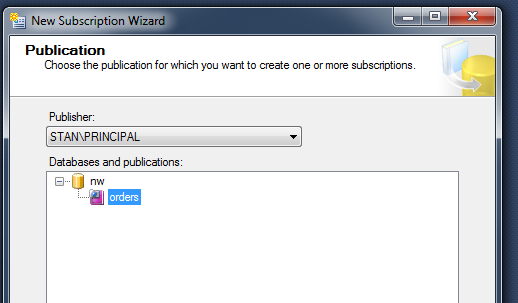
\includegraphics[width=0.75\linewidth,height=\textheight,keepaspectratio]{./images/img-031-021.png}

\begin{enumerate}
\def\labelenumi{\arabic{enumi}.}
\setcounter{enumi}{2}
\tightlist
\item
  Hozz létre egy másik, üres adatbázist \texttt{nw\_repl} névvel,
  szintén a PRIM szerveren.
\end{enumerate}

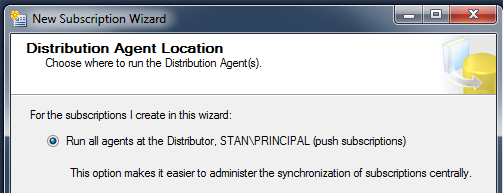
\includegraphics[width=0.75\linewidth,height=\textheight,keepaspectratio]{./images/img-031-022.png}

\begin{enumerate}
\def\labelenumi{\arabic{enumi}.}
\setcounter{enumi}{3}
\item
  Indítsd el az SQL Server Agent-et, ha nem fut.
\item
  A Replikáció → Terjesztés konfigurálása menüpont kiválasztásával
  állítsd be a PRIM-et saját terjesztőjeként. A pillanatfelvétel-mappa a
  következő lesz:

  \texttt{C:\textbackslash{}Program\ Files\textbackslash{}Microsoft\ SQL\ Server\textbackslash{}MSSQL14.PRIM\textbackslash{}MSSQL\textbackslash{}ReplData}
\end{enumerate}

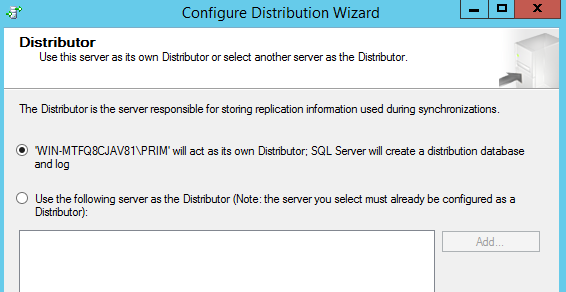
\includegraphics[width=0.75\linewidth,height=\textheight,keepaspectratio]{./images/img-027-014.png}

\begin{enumerate}
\def\labelenumi{\arabic{enumi}.}
\setcounter{enumi}{5}
\item
  Indítsd el az Új kiadvány varázslót, és válaszd ki a northwind
  adatbázist kiadványi adatbázisként.
\item
  A következő panelen válaszd a Pillanatkép-kiadvány típust, majd
  válaszd ki az Orders táblát a kiadvány egyetlen cikkeként.
\item
  A Táblaszűrő párbeszédpanelen kattints a Hozzáadás gombra.
\item
  Egészítsd ki a szűrési feltételt az amerikai ügyfelek szűréséhez:

\begin{Shaded}
\begin{Highlighting}[]
\KeywordTok{SELECT} \OperatorTok{\textless{}}\NormalTok{published\_columns}\OperatorTok{\textgreater{}} \KeywordTok{FROM}\NormalTok{ [dbo].[Orders]}
\KeywordTok{WHERE}\NormalTok{ ShipCountry }\OperatorTok{=} \StringTok{\textquotesingle{}USA\textquotesingle{}}
\end{Highlighting}
\end{Shaded}
\end{enumerate}

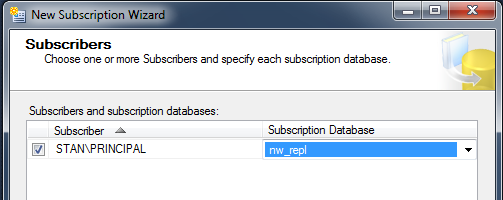
\includegraphics[width=0.75\linewidth,height=\textheight,keepaspectratio]{./images/img-031-023.png}

\begin{enumerate}
\def\labelenumi{\arabic{enumi}.}
\setcounter{enumi}{9}
\item
  Add meg, hogy a pillanatkép-ügynök kétpercenként fusson --- ehhez
  kattints a Módosítás gombra a következő panelen. \textbf{Megjegyzés:}
  \emph{ezt a rövid időintervallumot kizárólag bemutató célból
  alkalmazzuk. Az ügynök a \texttt{bcp} segédprogramot használja, amely
  az egész táblát zárolja a másolás ideje alatt, hogy garantálja az
  adatkonzisztenciát. Ez azt jelenti, hogy minden más tranzakció
  blokkolódik, amely módosítani szeretné a táblát. Éles rendszerekben a
  pillanatfelvétel-generálást a teljesítményre tekintettel kell
  ütemezni.}
\item
  Meg kell adni az ügynök biztonsági beállításait. A Security settings
  fülön add meg a saját felhasználói azonosítódat, és állítsd be a
  folyamatfiók megszemélyesítését. Ez a legegyszerűbb módja annak, hogy
  a pillanatkép-ügynök írási jogosultsággal rendelkezzen a
  pillanatfelvétel-mappára. \textbf{Megjegyzés:} gondolhatod, hogy miért
  futtatja az SQL Server Agent szolgáltatás vagy a SQLSERVER
  szolgáltatás alacsony jogosultságú, nem rendszergazdai
  Windows-fiókkal. Ennek az az oka, hogy így egy sikeres DBMS-feltörés
  esetén a támadónak kevesebb esélye van a teljes szerver
  kompromittálására.
\end{enumerate}

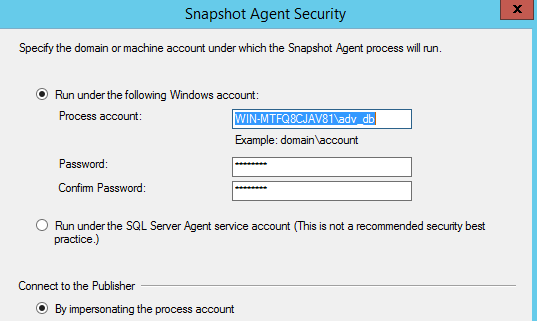
\includegraphics[width=0.75\linewidth,height=\textheight,keepaspectratio]{./images/img-030-019.png}

\begin{enumerate}
\def\labelenumi{\arabic{enumi}.}
\setcounter{enumi}{11}
\tightlist
\item
  A következő panelen válaszd a kiadvány létrehozását, és nevezd el
  `orders'-nek.
\end{enumerate}

\subsubsection{A kiadvány
ellenőrzése}\label{a-kiadvuxe1ny-ellenux151rzuxe9se}

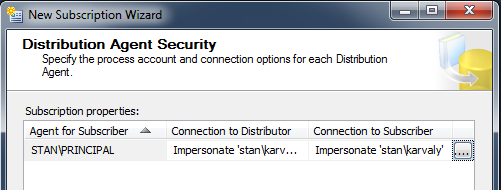
\includegraphics[width=0.75\linewidth,height=\textheight,keepaspectratio]{./images/img-032-024.png}

Az új kiadvány megjelenik a Helyi kiadványok csoportban. A
pillanatfelvétel-mappák itt jönnek létre:

\texttt{C:\textbackslash{}Program\ Files\textbackslash{}Microsoft\ SQL\ Server\textbackslash{}MSSQL14.PRIM\textbackslash{}MSSQL\textbackslash{}repldata\textbackslash{}unc\textbackslash{}WIN-MTFQ8CJAV81\$PRIM\_NORTHWIND\_TEST}

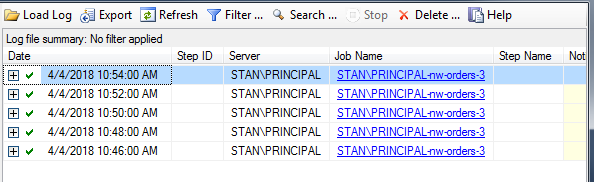
\includegraphics[width=0.75\linewidth,height=\textheight,keepaspectratio]{./images/img-030-020.png}

Tényleges pillanatfelvétel azonban még nem keletkezett, mert még nincs
feliratkozás, amelyet inicializálni kellene.

Ellenőrizd az SQL Server Agent feladatok között megjelenő új feladatot.
A feladatelőzmények (job history) mutatja, hogy az ügynök rendszeresen
lefut.

\subsubsection{Push feliratkozás
létrehozása}\label{push-feliratkozuxe1s-luxe9trehozuxe1sa}

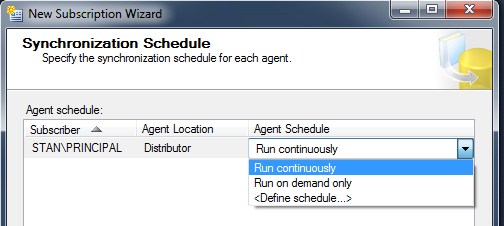
\includegraphics[width=0.75\linewidth,height=\textheight,keepaspectratio]{./images/img-032-025.png}

\begin{enumerate}
\def\labelenumi{\arabic{enumi}.}
\item
  Indítsd el az Új feliratkozás varázslót az orders kiadvány helyi
  menüjéből. Válaszd ki forrásként az orders kiadványt.
\item
  A következő panelen válaszd az összes ügynök futtatását a terjesztőn
  (push feliratkozás).
\item
  Add meg ugyanazt a szervert előfizetőként, és az \texttt{nw\_repl}
  adatbázist feliratkozási adatbázisként.
\item
  A terjesztési ügynök biztonságát állítsd be ugyanúgy, mint a
  pillanatkép-ügynöknél.
\item
  Az ütemezésnél válaszd a Folyamatos futtatás lehetőséget a minimális
  késleltetés érdekében.
\end{enumerate}

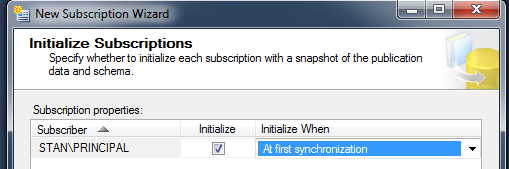
\includegraphics[width=0.75\linewidth,height=\textheight,keepaspectratio]{./images/img-032-026.png}

\begin{enumerate}
\def\labelenumi{\arabic{enumi}.}
\setcounter{enumi}{5}
\item
  A következő panelen válaszd az inicializálást. Ez elkészíti az első
  pillanatfelvételt a terjesztési mappában.
\item
  Fejezd be az új feliratkozás létrehozását.
\end{enumerate}

\textbf{Megjegyzés:} a feliratkozások és kiadványok tulajdonságait
később is módosíthatod, ha a helyi menüből a Tulajdonságok pontot
választod.

\subsubsection{A feliratkozás
ellenőrzése}\label{a-feliratkozuxe1s-ellenux151rzuxe9se}

\begin{enumerate}
\def\labelenumi{\arabic{enumi}.}
\tightlist
\item
  Keresd meg az Orders táblát az \texttt{nw\_repl} adatbázisban, és
  ellenőrizd, hogy tartalmazza-e az USA-s rendeléseket.
\end{enumerate}


\includegraphics[width=0.75\linewidth,height=\textheight,keepaspectratio]{./images/img-033-027.png}

\begin{enumerate}
\def\labelenumi{\arabic{enumi}.}
\setcounter{enumi}{1}
\item
  Ellenőrizd a pillanatfelvétel-mappa tartalmát. A \textbf{Bulk copy}
  egy gyors módszer, amellyel az SQL Server adatokat szúr be közvetlenül
  az adatbázisfájlokba. A mappában a következő fájlokat fogod látni:

  \begin{longtable}[]{@{}ll@{}}
  \toprule\noalign{}
  Fájlnév & Típus \\
  \midrule\noalign{}
  \endhead
  \bottomrule\noalign{}
  \endlastfoot
  Orders\_2.bcp & SQL Server Replication Snapshot Bulk-copy Data File \\
  Orders\_2.idx & SQL Server Replication Snapshot Index Script \\
  Orders\_2.pre & PRE File \\
  Orders\_2.sch & SQL Server Replication Snapshot Schema Script \\
  \end{longtable}
\item
  Indítsd el a replikációs monitort az új feliratkozás helyi menüjéből,
  és ellenőrizd a kiadvány és a feliratkozás állapotát. Az aktív
  replikációs ügynököket is itt tekintheted meg.
\item
  Nyisd meg a Feladat-aktivitás monitort. A terjesztési ügynök új
  feladatként jelenik meg a listában, amely folyamatosan fut.
\item
  Módosítsd UPDATE utasítással az Orders tábla első USA-s rekordját a
  közzétevőnél. A változás rövid időn belül (kb. 30 másodperccel)
  megjelenik a replikált táblában, miután a pillanatkép-ügynök
  legközelebb lefut.
\end{enumerate}

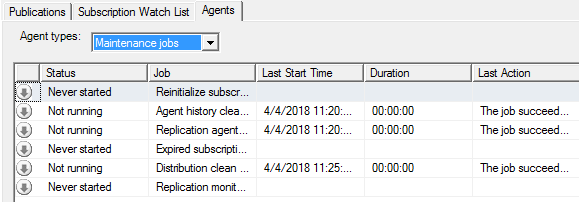
\includegraphics[width=0.75\linewidth,height=\textheight,keepaspectratio]{./images/img-033-028.png}

\begin{enumerate}
\def\labelenumi{\arabic{enumi}.}
\setcounter{enumi}{5}
\item
  Végül töröld a feliratkozást és a kiadványt. Ehhez válaszd a
  Replikáció csoport helyi menüjéből a Szkriptek generálása lehetőséget,
  add meg a `Törléshez\ldots{}' opciót, majd futtasd a szkriptet egy
  szerkesztőben. Alternatívaként egyenként is törölheted az
  objektumokat.
\item
  Az előfizetőnél lévő replikált táblák nem törlődnek a feliratkozás
  törlésekor, ezért az Orders táblát kézzel töröld az \texttt{nw\_repl}
  adatbázisból.
\end{enumerate}

\begin{quote}
\textbf{GYAKORLAT:} hozz létre push pillanatkép-kiadványt az
\texttt{nw\_repl} táblába, amely azokat az alkalmazottakat másolja az
Employees táblából, akiknek a beosztása „Sales Representative''.
Ellenőrizd a helyes működést, majd töröld az összes kapcsolódó
objektumot.
\end{quote}

\begin{center}\rule{0.5\linewidth}{0.5pt}\end{center}

\subsection{Tranzakciós
replikáció}\label{tranzakciuxf3s-replikuxe1ciuxf3}

\textbf{Forgatókönyv:} közel valós idejű (ütemezett) laza csatolást
szeretnénk létrehozni a központi Northwind adatbázis és egy külső
telephely között, amely csak az `Italok' (Beverages, CategoryID=1)
kategóriájú termékekkel foglalkozik. Csak az italos rendeléseket és
rendeléstételeket replikáljuk tranzakciós replikáción keresztül.

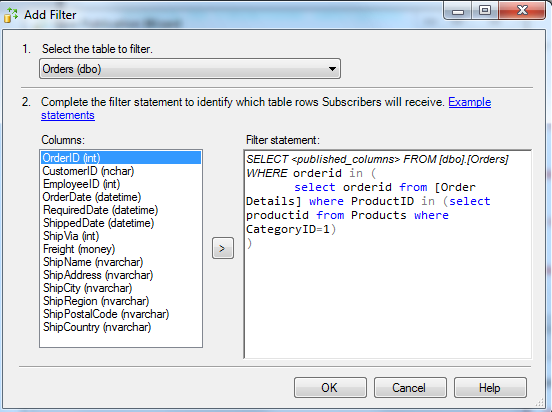
\includegraphics[width=0.75\linewidth,height=\textheight,keepaspectratio]{./images/img-034-029.png}

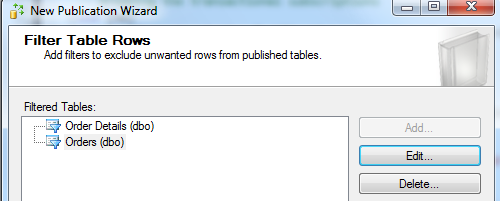
\includegraphics[width=0.75\linewidth,height=\textheight,keepaspectratio]{./images/img-035-030.png}

Ezt a demót először egyetlen szerveren (Principal) valósítjuk meg. A
fenti szűrési feltétel a következőképpen definiálható:

\begin{Shaded}
\begin{Highlighting}[]
\KeywordTok{select} \OperatorTok{*} \KeywordTok{from}\NormalTok{ [}\KeywordTok{Order}\NormalTok{ Details] }\KeywordTok{where}\NormalTok{ ProductID }\KeywordTok{in}\NormalTok{ (}\KeywordTok{select}\NormalTok{ productid }\KeywordTok{from}\NormalTok{ Products }\KeywordTok{where}
\NormalTok{CategoryID}\OperatorTok{=}\DecValTok{1}\NormalTok{)}

\KeywordTok{select} \OperatorTok{*} \KeywordTok{from}\NormalTok{ orders }\KeywordTok{where}\NormalTok{ orderid }\KeywordTok{in}\NormalTok{ (}
   \KeywordTok{select}\NormalTok{ orderid }\KeywordTok{from}\NormalTok{ [}\KeywordTok{Order}\NormalTok{ Details] }\KeywordTok{where}\NormalTok{ ProductID }\KeywordTok{in}\NormalTok{ (}\KeywordTok{select}\NormalTok{ productid }\KeywordTok{from}
\NormalTok{Products }\KeywordTok{where}\NormalTok{ CategoryID}\OperatorTok{=}\DecValTok{1}\NormalTok{)}
\NormalTok{)}
\end{Highlighting}
\end{Shaded}

\begin{enumerate}
\def\labelenumi{\arabic{enumi}.}
\item
  A replikációs konfigurációt visszaállíthatod a Terjesztés és
  közzététel letiltása lehetőség kiválasztásával a Replikáció menüből.
\item
  A kiadványtípus párbeszédpanelen add meg a kiadvány típusaként a
  Tranzakciós típust.
\item
  A Cikkek panelen válaszd ki az Orders és az Order Details táblákat.
\item
  A Táblaszűrő panelen add hozzá a szűrőt mindkét táblához egyenként, a
  fenti lekérdezések WHERE részének bemásolásával. Az Orders táblához:

\begin{Shaded}
\begin{Highlighting}[]
\KeywordTok{SELECT} \OperatorTok{\textless{}}\NormalTok{published\_columns}\OperatorTok{\textgreater{}} \KeywordTok{FROM}\NormalTok{ [dbo].[Orders]}
\KeywordTok{WHERE}\NormalTok{ orderid }\KeywordTok{in}\NormalTok{ (}
      \KeywordTok{select}\NormalTok{ orderid }\KeywordTok{from}\NormalTok{ [}\KeywordTok{Order}\NormalTok{ Details] }\KeywordTok{where}\NormalTok{ ProductID }\KeywordTok{in}\NormalTok{ (}\KeywordTok{select}\NormalTok{ productid }\KeywordTok{from}
\NormalTok{Products }\KeywordTok{where}\NormalTok{ CategoryID}\OperatorTok{=}\DecValTok{1}\NormalTok{)}
\NormalTok{)}
\end{Highlighting}
\end{Shaded}
\item
  Mindkét táblára legyen definiálva a szűrő.
\item
  A következő panelen válaszd a Pillanatfelvétel azonnali létrehozása
  lehetőséget.
\item
  A következő paneleken állítsd be az ügynökök biztonságát az előző
  demóhoz hasonlóan.
\item
  Nevezd el a kiadványt \texttt{nw\_trans} névvel, és fejezd be a
  kiadvány létrehozását.
\end{enumerate}

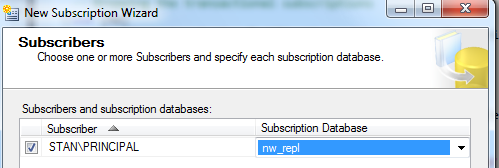
\includegraphics[width=0.75\linewidth,height=\textheight,keepaspectratio]{./images/img-035-031.png}

\begin{enumerate}
\def\labelenumi{\arabic{enumi}.}
\setcounter{enumi}{8}
\item
  A kiadvány helyi menüjéből válaszd az Új feliratkozás lehetőséget.
\item
  A következő panelen válaszd az összes ügynök futtatását a Terjesztőn
  (push feliratkozás).
\end{enumerate}

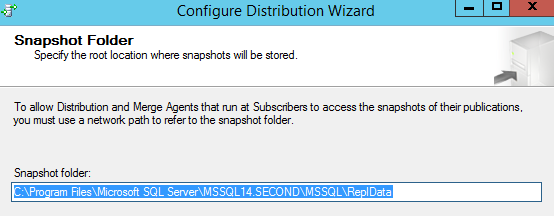
\includegraphics[width=0.75\linewidth,height=\textheight,keepaspectratio]{./images/img-037-034.png}

\begin{enumerate}
\def\labelenumi{\arabic{enumi}.}
\setcounter{enumi}{10}
\item
  Válaszd ki az \texttt{nw\_repl} adatbázist feliratkozási
  adatbázisként.
\item
  A terjesztési ügynök biztonságát állítsd be az előző demóhoz
  hasonlóan.
\item
  A naplóolvasó és terjesztési ügynök ütemezéseként add meg a Folyamatos
  futtatást.
\item
  Az Inicializálás feliratkozások panelen válaszd az Azonnal
  lehetőséget.
\end{enumerate}

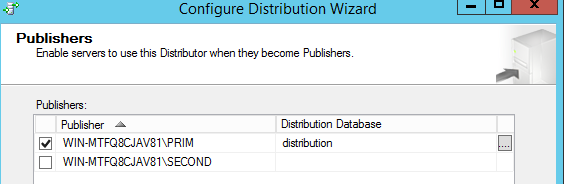
\includegraphics[width=0.75\linewidth,height=\textheight,keepaspectratio]{./images/img-037-035.png}

\begin{enumerate}
\def\labelenumi{\arabic{enumi}.}
\setcounter{enumi}{14}
\tightlist
\item
  Teszteld a tranzakciós replikáció helyes működését. Frissítsd az
  employeeID mezőt az Orders tábla első rekordjában a northwind
  adatbázisban, majd válaszd ki ugyanazt a rekordot az \texttt{nw\_repl}
  adatbázisban. A módosult értéknek 10 másodpercen belül meg kell
  jelennie.
\end{enumerate}

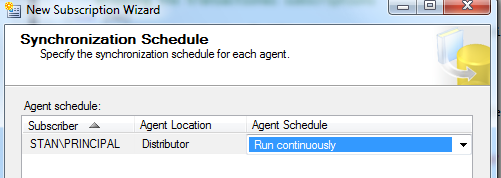
\includegraphics[width=0.75\linewidth,height=\textheight,keepaspectratio]{./images/img-035-032.png}

\begin{enumerate}
\def\labelenumi{\arabic{enumi}.}
\setcounter{enumi}{15}
\item
  Ellenőrizd a replikációs ügynökök működését.
\item
  Takarítsd el a replikációt az összes replikációs objektum törlésével.
\end{enumerate}

\begin{quote}
\textbf{GYAKORLAT:} valósítsd meg a laza csatolásos rendelésfeldolgozási
forgatókönyvet tranzakciós replikáció segítségével a Products, Orders és
Order Details táblákon. Használd a fenti háromszerveres konfigurációt,
ahol SECOND a terjesztő. Tételezzük fel, hogy a logisztikai részlegnek
saját adatbázisa van, amely a THIRD szerveren fut.

\begin{enumerate}
\def\labelenumi{\arabic{enumi}.}
\tightlist
\item
  Adj hozzá egy `status' nevű mezőt az Orders táblához a PRIM példány
  northwind adatbázisában, alapértelmezett értéke legyen 0.
\item
  Módosítsd a meglévő rendelések állapotát 0-ról 2-re. Nem akarjuk az
  összes meglévő rendelést feldolgozni.
\item
  Replikáld a három táblát az \texttt{nw\_repl} adatbázisba tranzakciós
  replikáció segítségével.
\item
  Mivel az előfizető módosíthatja a replikált rekordokat, és a
  kereskedési alkalmazás az Orders táblán \emph{soha} nem frissíti a
  status mezőt, ezt a mezőt az előfizetőn arra fogjuk használni, hogy a
  rendelési rekordok feldolgozási állapotát naplózzuk --- hasonlóan az
  esettanulmány megoldásához. Így elkerülünk egy extra naplótáblát.
  Részletek:

  \begin{itemize}
  \tightlist
  \item
    \begin{enumerate}
    \def\labelenumii{\alph{enumii}.}
    \tightlist
    \item
      Tudjuk, hogy az új rendelések alapértelmezetten 0 állapotúak
      lesznek. A módosított rendelések megjelöléséhez egy frissítési
      triggert alkalmazhatunk a közzétevőn, amely a már meglévő rekord
      állapotát 1-re változtatja.
    \end{enumerate}
  \item
    \begin{enumerate}
    \def\labelenumii{\alph{enumii}.}
    \setcounter{enumii}{1}
    \tightlist
    \item
      Az előfizetőn futó feladat 0 vagy 1 állapotú rendelési rekordokat
      dolgoz fel, és sikeres feldolgozás esetén az állapotot 2-re
      állítja.\footnote{Ez jól működik, ha a rendelést csak egyszer
        frissítik a közzétevő oldalon.}
    \end{enumerate}
  \end{itemize}
\item
  Valósítsd meg és teszteld a megoldást.
\item
  Töröld a kiadványt és a feliratkozást.
\end{enumerate}
\end{quote}

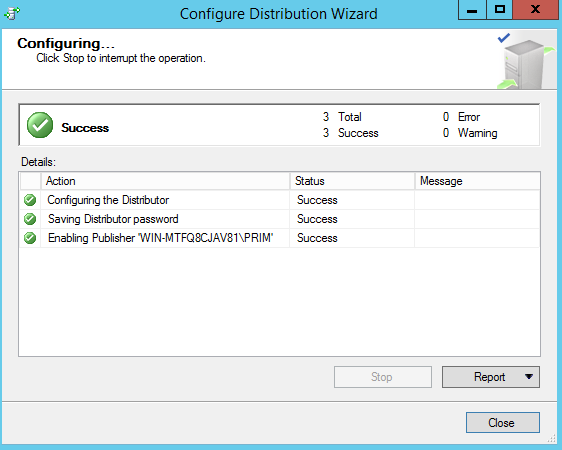
\includegraphics[width=0.75\linewidth,height=\textheight,keepaspectratio]{./images/img-038-036.png}

\begin{center}\rule{0.5\linewidth}{0.5pt}\end{center}

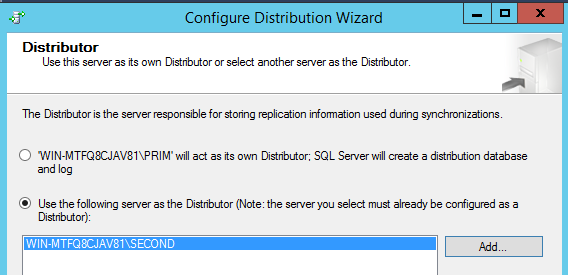
\includegraphics[width=0.75\linewidth,height=\textheight,keepaspectratio]{./images/img-038-037.png}

\subsection[Replikáció különálló szerverek
között]{\texorpdfstring{Replikáció különálló szerverek
között\footnote{Az SQL Server 2019 és Windows 10 rendszerek egy hibája
  miatt a varázsló az \texttt{sp\_adddistributor} segítségével ---
  távoli terjesztő esetén --- üres jelszót használ a megadott helyett,
  és a 21768-as kivételt adja vissza („The password specified for the
  @password parameter must be the same when the procedure is executed at
  the Publisher and at the Distributor''). A demo futtatásához add meg
  manuálisan a jelszót az \texttt{sp\_adddistributor} hívásában:
  \texttt{use\ master} /
  \texttt{exec\ sp\_adddistributor\ @distributor\ =\ \textquotesingle{}DESKTOP-....\textbackslash{}SECOND\textquotesingle{},\ @password\ =\ \textquotesingle{}type\ password\ here\textquotesingle{}}}}{Replikáció különálló szerverek között}}\label{replikuxe1ciuxf3-kuxfcluxf6nuxe1lluxf3-szerverek-kuxf6zuxf6tt4}

A következő demóban ugyanezt a tranzakciós replikációt valósítjuk meg
egy reálisabb forgatókönyvben: a PRIM a közzétevő, a SECOND a terjesztő,
a THIRD az előfizető. Még reálisabb esetben nemcsak különálló
szerverpéldányok lennének, hanem különálló szervergépeken is futna
mindegyik --- ilyen konfigurációt a laborban nem tudunk megvalósítani.

\subsubsection{A terjesztő
konfigurálása}\label{a-terjesztux151-konfiguruxe1luxe1sa}

\begin{enumerate}
\def\labelenumi{\arabic{enumi}.}
\item
  Indítsd el a SECOND és THIRD példányokat, és az SQL Server Agent-et a
  SECOND példányon.
\item
  Állítsd vissza a replikációs konfigurációt a PRIM-en a Terjesztés és
  közzététel letiltása lehetőség kiválasztásával a Replikáció menüből.
\item
  A SECOND példányon a Replikáció helyi menüjéből válaszd a Terjesztés
  konfigurálása lehetőséget, és fogadd el az első választást. Ez
  létrehozza a terjesztési adatbázist a SECOND-on.
\item
  A következő panelen add meg, hogy a Server Agent-et manuálisan
  indítjuk.
\item
  A következő panelen fogadd el a pillanatfelvétel-mappa elérési útját:

  \texttt{C:\textbackslash{}Program\ Files\textbackslash{}Microsoft\ SQL\ Server\textbackslash{}MSSQL14.SECOND\textbackslash{}MSSQL\textbackslash{}ReplData}
\item
  A következő panelen fogadd el az alapértelmezéseket a terjesztési
  adatbázis helyéhez és nevéhez.
\item
  Ezután meg kell adni, hogy mely közzétevő szerverek jogosultak ezt a
  terjesztési adatbázist használni. A következő panelen szüntesd meg a
  SECOND kijelölését (mivel a SECOND nem fog közzétenni), majd az
  Hozzáadás gombbal add hozzá a PRIM példányt.
\item
  A következő panelen meg kell adni egy jelszót, amelyet a PRIM
  közzétevők fognak használni ehhez a terjesztési adatbázishoz. Add meg
  ugyanazt a jelszót, amelyet a bejelentkezéshez használsz. Erre a
  jelszóra később szükség lesz.
\item
  A folyamat végén sikeresen konfigurálta a terjesztőt.
\end{enumerate}

\subsubsection{A közzétevő
konfigurálása}\label{a-kuxf6zzuxe9tevux151-konfiguruxe1luxe1sa}

\begin{enumerate}
\def\labelenumi{\arabic{enumi}.}
\item
  A PRIM konfigurálásához először letiltjuk azt terjesztőként. Ne
  feledd, hogy eddig a PRIM saját terjesztőjeként működött. A Replikáció
  helyi menüjéből válaszd a Terjesztés és közzététel letiltása
  lehetőséget. Miután a PRIM-et letiltottuk terjesztőként, a helyi menü
  megváltozik. Válaszd most a Terjesztés konfigurálása lehetőséget, és
  add meg a SECOND példányt a PRIM terjesztőjeként.
\item
  A következő panelen add meg ugyanazt a jelszót, mint korábban (a 8.
  lépésben).
\item
  A terjesztés most be van állítva.
\end{enumerate}

\subsubsection{A kiadvány és a feliratkozás
hozzáadása}\label{a-kiadvuxe1ny-uxe9s-a-feliratkozuxe1s-hozzuxe1aduxe1sa}

\begin{enumerate}
\def\labelenumi{\arabic{enumi}.}
\item
  Hozd létre a tranzakciós kiadványt a PRIM-en a szokásos módon (Orders
  tábla szűrő nélkül).
\item
  A THIRD-en ne konfiguráljuk a Terjesztési tulajdonságokat, mert a
  THIRD nem fog közzétenni.
\item
  Hozz létre új feliratkozást a THIRD példányon a Helyi feliratkozások →
  Hozzáadás menüponttal. Válaszd ki a PRIM-et közzétevőként, és válaszd
  ki az előző lépésben létrehozott kiadványt.
\item
  Válaszd az összes ügynök futtatása a Terjesztőn lehetőséget.
\item
  A varázsló a THIRD-en új adatbázisként hozhatja létre a feliratkozási
  adatbázist \texttt{nw\_repl} névvel.
\item
  Teszteld a feliratkozást. Nyiss egy lekérdezésszerkesztőt a PRIM-en,
  és frissíts egy rekordot az Orders táblában. Nyiss egy
  lekérdezésszerkesztőt a THIRD-en, és ellenőrizd, hogy a módosítás 10
  másodpercen belül megjelenik-e a replikált táblában.
\end{enumerate}

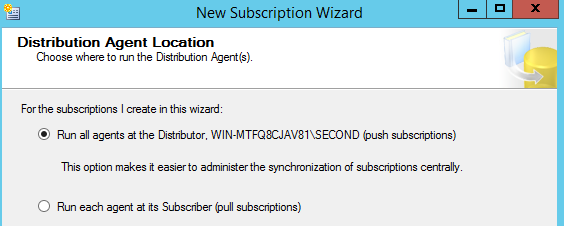
\includegraphics[width=0.75\linewidth,height=\textheight,keepaspectratio]{./images/img-039-038.png}

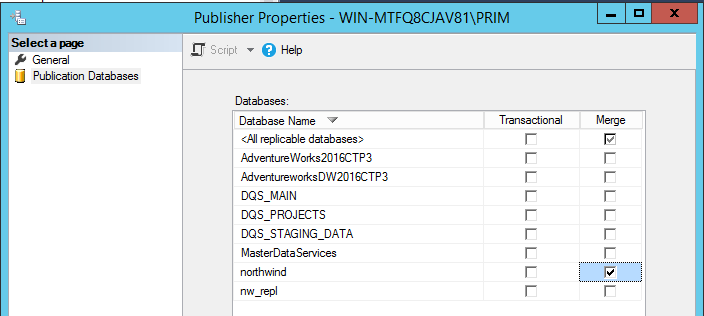
\includegraphics[width=0.75\linewidth,height=\textheight,keepaspectratio]{./images/img-042-042.png}

\begin{enumerate}
\def\labelenumi{\arabic{enumi}.}
\setcounter{enumi}{6}
\tightlist
\item
  Töröld a kiadványt a PRIM-en és a feliratkozást a THIRD-en. Töröld a
  replikált táblát a THIRD-en.
\end{enumerate}

\begin{quote}
\textbf{GYAKORLAT:} valósítsd meg a laza csatolásos rendelésfeldolgozási
forgatókönyvet tranzakciós replikáció segítségével a Products, Orders és
Order Details táblákon. Használd a fenti háromszerveres konfigurációt,
ahol SECOND a terjesztő. Tételezzük fel, hogy a logisztikai részlegnek
saját adatbázisa van, amely a THIRD szerveren fut.

\begin{enumerate}
\def\labelenumi{\arabic{enumi}.}
\tightlist
\item
  Adj hozzá egy `status' nevű mezőt az Orders táblához a PRIM példány
  northwind adatbázisában, alapértelmezett értéke legyen 0.
\item
  Módosítsd a meglévő rendelések állapotát 0-ról 2-re. Nem akarjuk az
  összes meglévő rendelést feldolgozni.
\item
  Replikáld a három táblát az \texttt{nw\_repl} adatbázisba tranzakciós
  replikáció segítségével.
\item
  Mivel az előfizető módosíthatja a replikált rekordokat, és a
  kereskedési alkalmazás az Orders táblán \emph{soha} nem frissíti a
  status mezőt, ezt a mezőt az előfizetőn a rendelési rekordok
  feldolgozási állapotának naplózására fogjuk használni --- hasonlóan az
  esettanulmány megoldásához. Részletek:

  \begin{itemize}
  \tightlist
  \item
    \begin{enumerate}
    \def\labelenumii{\alph{enumii}.}
    \tightlist
    \item
      Tudjuk, hogy az új rendelések alapértelmezetten 0 állapotúak
      lesznek. A módosított rendelések megjelöléséhez egy frissítési
      triggert alkalmazhatunk a közzétevőn, amely a már meglévő rekord
      állapotát 1-re változtatja.\footnote{Ez jól működik, ha a
        rendelést csak egyszer frissítik a közzétevő oldalon.}
    \end{enumerate}
  \item
    \begin{enumerate}
    \def\labelenumii{\alph{enumii}.}
    \setcounter{enumii}{1}
    \tightlist
    \item
      Az előfizetőn futó feladat 0 vagy 1 állapotú rendelési rekordokat
      dolgoz fel, és sikeres feldolgozás esetén az állapotot 2-re
      állítja.
    \end{enumerate}
  \end{itemize}
\item
  Valósítsd meg és teszteld a megoldást.
\item
  Töröld a kiadványt és a feliratkozást.
\end{enumerate}
\end{quote}

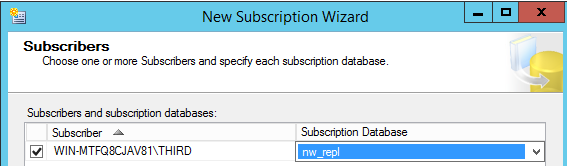
\includegraphics[width=0.75\linewidth,height=\textheight,keepaspectratio]{./images/img-039-039.png}

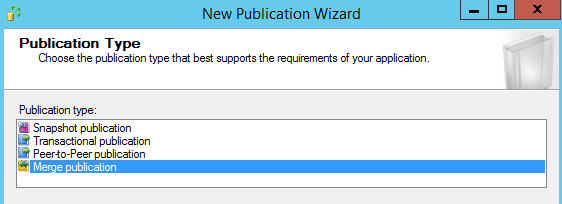
\includegraphics[width=0.75\linewidth,height=\textheight,keepaspectratio]{./images/img-042-043.png}

\begin{center}\rule{0.5\linewidth}{0.5pt}\end{center}

\subsection{Peer-to-Peer tranzakciós
replikáció}\label{peer-to-peer-tranzakciuxf3s-replikuxe1ciuxf3}

Bármely csomópontba írt módosítások automatikusan és csak egyszer
terjednek az összes többi csomópontra. Horizontális (scale-out) olvasási
terheléselosztásra tervezték. Az azonos rekord egyidejű írásai több
csomóponton --- azaz írási konfliktusok --- nem engedélyezettek, és
kritikus hibaként kezelik őket, amelyek kézi beavatkozást
igényelnek.\footnote{Lásd:
  https://learn.microsoft.com/en-us/sql/relational-databases/replication/transactional/peer-to-peer-transactional-replication}

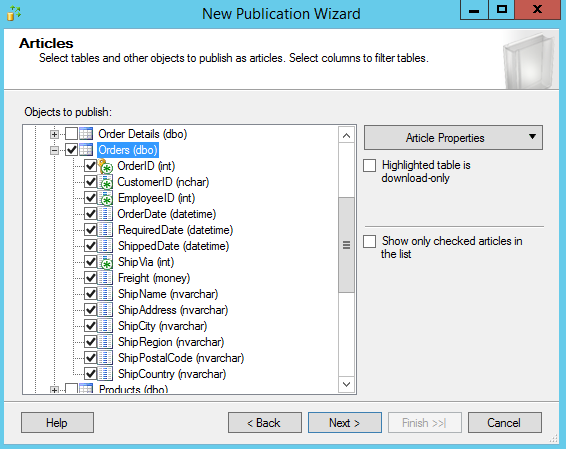
\includegraphics[width=0.75\linewidth,height=\textheight,keepaspectratio]{./images/img-043-044.png}

\begin{center}\rule{0.5\linewidth}{0.5pt}\end{center}

\subsection{Összefésülő
replikáció}\label{uxf6sszefuxe9suxfclux151-replikuxe1ciuxf3}

\textbf{Forgatókönyv:} az értékesítési munkatársak utaznak, és új
rendeléseket vesznek fel az ügyfeleknek. Alkalmanként módosítani kell
korábbi rendeléseket is, például ha megváltozik a szállítási cím.
Előfordulhat az is, hogy két alkalmazott egyszerre módosítja ugyanazt a
rendelést. A munkatársak nem folyamatosan kapcsolódnak az internethez.
Olyan replikációs megoldást kell tervezni, amely az összes ilyen
módosítást összefésüli egymással és a központi Northwind adatbázissal.

Az \textbf{összefésülő replikációban} a naplóolvasó ügynök szerepét
triggerek, táblák és nézetek veszik át, amelyeket automatikusan hoznak
létre minden előfizető adatbázisban és a közzétevő adatbázisban is. A
triggerek az \texttt{MSmerge\_*} nevű speciális rendszertáblákba
naplózzák a változásokat --- ezek a táblák ugyanabban az adatbázisban
jönnek létre, mint a replikált tábla. Minden táblához három trigger jön
létre: \texttt{MSmerge\_{[}ins,\ upd,\ del{]}\_*}. Vannak adatbázis
szintű \emph{sématriggerek} is, amelyek a replikált táblák sémájának
változásait naplózzák.

Az összefésülő replikáció egy pillanatkép-ügynök által készített kezdeti
pillanatfelvétellel indul. Alapértelmezés szerint a pillanatkép-ügynök
14 naponta fut. Ezután az összefésülési ügynök feladata hasonló a
terjesztési ügynökéhez, azzal a különbséggel, hogy az összefésülő
replikáció alapértelmezetten kétirányúra van konfigurálva. Ez azt
jelenti, hogy az ügynök az előfizetői és a közzétevői oldalon is
alkalmazza a változásokat. Minden feliratkozáshoz külön összefésülési
ügynök tartozik. Az összefésülési ügynök push feliratkozás esetén a
terjesztőn fut, pull feliratkozás esetén az előfizetőn.

A terjesztési adatbázis csak előzményeket és hibainformációkat tárol.

A kétirányú adatszinkronizáció támogatásához az összefésülő replikáció
cikkeinek UNIQUEIDENTIFIER (GUID) típusú oszloppal kell rendelkezniük,
amely hasonlóan működik az identity adattípushoz, de globálisan egyedi
értékeket generál.\footnote{Megjegyzés: az elosztott
  adatbázis-rendszerek bármely megfigyelési időpontban inkonzisztensek
  lehetnek, de a szinkronizálási mechanizmus garantálja, hogy ha nem
  következik be további frissítési esemény, egy globális konzisztencia
  (konszenzus) elérésre kerül egy idő után. Ezt nevezzük
  \textbf{végleges konzisztenciának} (eventual consistency). A CAP-tétel
  szerint a C, A, P tulajdonságok egyszerre nem teljesíthetők teljes
  mértékben egyetlen elosztott adatbázis-rendszerben sem: Konzisztencia
  (minden olvasás a legutóbbi írást vagy hibát kapja), Rendelkezésre
  állás (minden olvasás tartalmaz adatokat, de lehet nem a legfrissebb),
  Partíciótűrés (a rendszer hálózati hibák esetén is működik) --- mivel
  hálózati hibák előfordulhatnak, a konzisztencia és a rendelkezésre
  állás közötti kompromisszumot az alkalmazás követelményei alapján kell
  eldönteni. A bemutatott összefésülési folyamat a rendelkezésre állást
  részesíti előnyben a konzisztenciával szemben.} Ha ilyen oszlop nem
létezik, automatikusan hozzáadódik a táblákhoz --- ez azonban
összeomlaszthatja a már meglévő, a táblát használó alkalmazásokat. Az új
mező törlődik, amikor a kiadványt törlik.

A szinkronizálási folyamat részletei nem szerepelnek ebben a
tankönyvben.\footnote{Lásd:
  https://documentation.help/replsql/repltypes\_30z7.htm}

\subsubsection{A kiadvány}\label{a-kiadvuxe1ny}

\begin{quote}
\textbf{GYAKORLAT:} a megoldás kidolgozásához kövesd az alábbi
lépéseket.
\end{quote}

\begin{enumerate}
\def\labelenumi{\arabic{enumi}.}
\item
  Állítsd be a SECOND példányt közzétevőként, még ha nem is fog
  kiadványokat közzétenni --- enélkül a feloldók listája nem lesz
  elérhető:
\item
  Konfiguráld a SECOND példányt a PRIM terjesztőjeként (lásd az előző
  részt). Ezt követően a PRIM-en ezt kell látnod.
\end{enumerate}

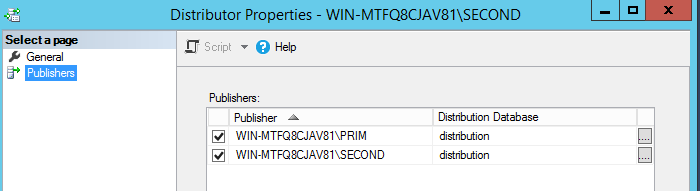
\includegraphics[width=0.75\linewidth,height=\textheight,keepaspectratio]{./images/img-041-040.png}

\begin{enumerate}
\def\labelenumi{\arabic{enumi}.}
\setcounter{enumi}{2}
\item
  Engedélyezd a northwind adatbázist összefésülő replikációhoz. Válaszd
  ki a Kiadványi adatbázisok fület a közzétevőn (PRIM).
\item
  Válaszd ki a northwind adatbázist kiadványi adatbázisként, és válaszd
  ki a kiadvány típusát: \textbf{Összefésülő kiadvány} (Merge
  publication).
\item
  Fogadd el az alapértelmezett előfizető-típusokat, és válaszd ki az
  Orders táblát a kiadvány egyetlen cikkeként.
\item
  Minden cikkhez különféle tulajdonságokat állíthatsz be a
  Cikktulajdonságok kiválasztásával, beleértve a különböző
  konfliktustípusokhoz használandó feloldót is. Konfliktus akkor
  keletkezik, amikor egy ügynök olyan rekordot próbál módosítani,
  amelynek van egy függőben lévő módosítása. A jelenleg a szerveren
  regisztrált beépített feloldó modulokat az
  \texttt{sp\_enumcustomresolvers} eljárással listázhatod. A beépített
  feloldók szükséges paramétereit lásd a lábjegyzetben.\footnote{Lásd:
    https://learn.microsoft.com/en-us/sql/relational-databases/replication/merge/advanced-merge-replication-conflict-com-based-resolvers}
  Saját feloldót is hozzáadhatsz tárolt eljárásként vagy
  DLL-ként.\footnote{Lásd:
    https://learn.microsoft.com/en-us/sql/relational-databases/replication/implement-a-custom-conflict-resolver-for-a-merge-article
    --- Az egyéni feloldó eljárás a Közzétevőn fut, és az Összefésülési
    ügynök hívja meg. Lekérdezi a megváltozott rekordot az Előfizetőtől
    az Összefésülési ügynöktől kapott sor GUID segítségével, és egy
    egysoros eredményhalmazt ad vissza, amely ugyanolyan mezőkkel
    rendelkezik, mint az alaptábla, és a nyertes rekord értékeit
    tartalmazza.} Az alapértelmezett feloldó a \textbf{„amelyik elsőként
  ér a közzétevőhöz, az nyer''} (first to Publisher wins) stratégiát
  valósítja meg:
\end{enumerate}

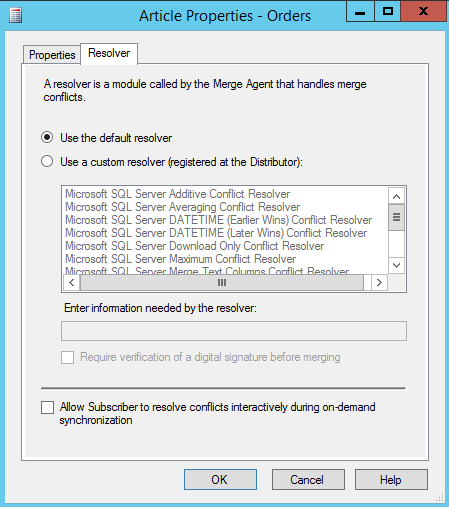
\includegraphics[width=0.75\linewidth,height=\textheight,keepaspectratio]{./images/img-044-045.png}

\begin{itemize}
\tightlist
\item
  \begin{enumerate}
  \def\labelenumi{\alph{enumi}.}
  \tightlist
  \item
    Ha a konfliktus egy közzétevő és egy előfizető között lép fel, a
    közzétevő változása kerül elfogadásra, az előfizető értékét
    elutasítják.
  \end{enumerate}
\item
  \begin{enumerate}
  \def\labelenumi{\alph{enumi}.}
  \setcounter{enumi}{1}
  \tightlist
  \item
    Ha a konfliktus két előfizető között lép fel pull feliratkozás
    esetén, az első előfizető változása kerül elfogadásra, amelyik
    szinkronizál a közzétevővel, a többi elutasításra kerül.
  \end{enumerate}
\end{itemize}

\begin{enumerate}
\def\labelenumi{\arabic{enumi}.}
\setcounter{enumi}{6}
\item
  A következő panel figyelmeztet, hogy egy új GUID-ot adnak hozzá a
  táblához. Ez nem változtatja meg a tábla elsődleges kulcs és idegen
  kulcs megszorításait.
\item
  A pillanatkép-ügynök ütemezéséhez fogadd el az alapértelmezéseket,
  majd az ügynök biztonságát a szokásos módon állítsd be.
\end{enumerate}

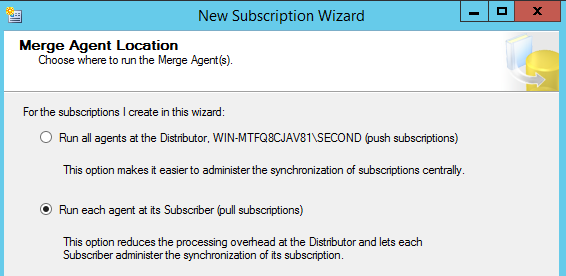
\includegraphics[width=0.75\linewidth,height=\textheight,keepaspectratio]{./images/img-046-048.png}

\begin{enumerate}
\def\labelenumi{\arabic{enumi}.}
\setcounter{enumi}{8}
\tightlist
\item
  Nevezd el a kiadványt \texttt{nw\_merge} névvel, és hozd létre.
  Ellenőrizd az új GUID-oszlopot és a 3 új triggert az Orders táblán.
\end{enumerate}

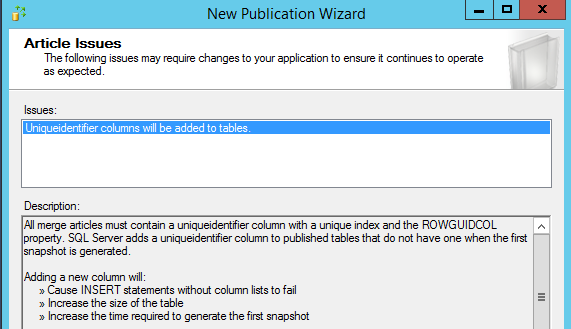
\includegraphics[width=0.75\linewidth,height=\textheight,keepaspectratio]{./images/img-045-046.png}

\subsubsection{A feliratkozás}\label{a-feliratkozuxe1s}

Két előfizetőt adunk hozzá az összefésülési folyamat bemutatásához.

\begin{enumerate}
\def\labelenumi{\arabic{enumi}.}
\item
  Indítsd el az SQL Server Agent-et a THIRD példányon manuálisan.
\item
  A THIRD példányon válaszd az Új feliratkozás lehetőséget, és add meg a
  PRIM-et közzétevőként.
\item
  A következő panelen válaszd a pull feliratkozást. Ez megfelel a
  szokásos elvárásnak, hogy az előfizetők maguk szeretnék ütemezni a
  szinkronizálást.
\item
  Add hozzá mindkét előfizetőt: egyet a THIRD példányon, egyet a
  PRIM-en, újonnan létrehozott adatbázisokkal \texttt{nw\_merge\_1-2}
  névvel.
\end{enumerate}

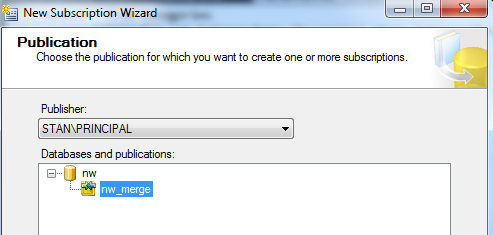
\includegraphics[width=0.75\linewidth,height=\textheight,keepaspectratio]{./images/img-045-047.png}

\begin{enumerate}
\def\labelenumi{\arabic{enumi}.}
\setcounter{enumi}{4}
\item
  Az ügynökök biztonságát a szokásos módon állítsd be.
\item
  Mindkét összefésülési ügynök szinkronizálási ütemezését állítsd
  „Folyamatos futtatás''-ra. \emph{Megjegyzés: ez csak teszt és bemutató
  célokra szól. Valós esetben az összefésülési folyamat meghatározott
  időközönként vagy igény szerint indulna el, amikor egy meghatározott
  esemény --- például VPN-kapcsolat --- létrejön az előfizetőn.}
\end{enumerate}

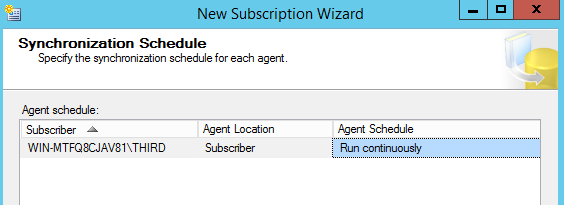
\includegraphics[width=0.75\linewidth,height=\textheight,keepaspectratio]{./images/img-046-049.png}

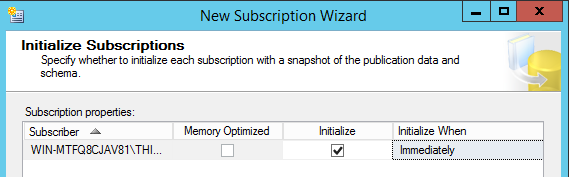
\includegraphics[width=0.75\linewidth,height=\textheight,keepaspectratio]{./images/img-047-050.png}

\begin{enumerate}
\def\labelenumi{\arabic{enumi}.}
\setcounter{enumi}{6}
\item
  Inicializáld a feliratkozásokat azonnal.
\item
  Összefésülő kiadványban az előfizetők újra közzétehetik azt a
  kiadványt, amelyre feliratkoztak (Server típusú feliratkozás), így
  hierarchikus feliratkozási architektúrát hozva létre. A Server típusú
  feliratkozás lehetővé teszi explicit numerikus prioritás
  hozzárendelését is minden szerverhez, amelyet konfliktus esetén
  használnak. Válaszd a Client típusú feliratkozást.
\item
  Véglegesítsd és indítsd el a replikációt.
\item
  Ellenőrizd, hogy a módosított értékek az összes többi előfizetőhöz és
  közzétevőhöz is eljutnak-e: szerkeszd meg az Orders táblát három
  különböző szerkesztőben. Légy türelmes: a szinkronizálás akár 2 percig
  is tarthat.\footnote{Elosztott adatbázis-rendszerek bármely
    megfigyelési időpontban inkonzisztensek lehetnek, de a
    szinkronizálási mechanizmus garantálja, hogy ha nem következik be
    további frissítési esemény, egy globális konzisztencia elérésébe
    kerül egy idő után --- ez a \textbf{végleges konzisztencia}. Lásd:
    https://www.bmc.com/blogs/cap-theorem/}
\item
  Teszteld az alapértelmezett első-érkező-nyer (first-come-first-served)
  konfliktusfeloldást, amikor a két előfizető `egyidejűleg' frissít egy
  rekordot (figyelembe véve, hogy az ügynökök percenként lekérdezik a
  naplókat). Az a módosítási kérés kerül elfogadásra, amelyik elsőként
  ér el a Közzétevő adatbázisba. Használd az SSMS Ablak → Vízszintes
  lapcsoportok hozzáadása parancsát, hogy mindhárom táblát egyszerre
  lásd. Az adatrácsokat a Ctrl+R megnyomásával frissítheted.
\end{enumerate}

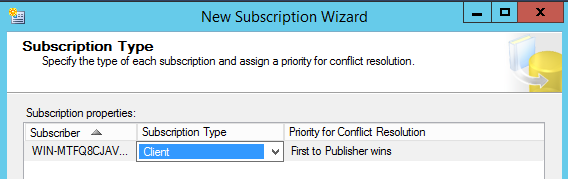
\includegraphics[width=0.75\linewidth,height=\textheight,keepaspectratio]{./images/img-047-051.png}

\begin{enumerate}
\def\labelenumi{\arabic{enumi}.}
\setcounter{enumi}{11}
\item
  Az összefésülési konfliktusokat a Replikáció-konfliktus megtekintő
  eszközben tekintheted meg és oldhatod fel manuálisan, amely elérhető a
  kiadvány helyi menüjéből. Ha egy rekordot mindhárom szerver frissített
  --- vagyis a konfliktus 3 felet érint ---, két különálló
  konfliktusként jelenik meg, ugyanazzal a nyertessel. Elfogadhatod az
  alapértelmezett feloldást (Submit Winner gombra kattintva) vagy
  visszafordíthatod (Submit Loser).
\item
  A szinkronizálási folyamat aktuális állapotát a feliratkozás helyi
  menüjéből a Szinkronizálási állapot megtekintése lehetőséggel
  ellenőrizheted. A folyamatot manuálisan is elindíthatod.
\item
  Mindkét példányon generálj és tekints meg replikációs szkripteket a
  Replikáció csoport helyi menüjéből a Szkriptek generálása lehetőség
  kiválasztásával.
\item
  Töröld az összes replikációs objektumot.
\end{enumerate}

\begin{quote}
\textbf{GYAKORLAT:} az új forgatókönyvben az alkalmazottak a Northwind
adatbázis Products táblájának UnitPrice mezőjét frissítik, és az
egyidejű módosítások összefésülnek. Az egyik alkalmazottnak alacsonyabb
prioritása van, mint a másiknak. Állíts be összefésülő kiadványt a
PRIM-ről pull feliratkozásokkal a SECOND-on és a THIRD-ön. A Server
típusú feliratkozás segítségével állítsd be a prioritást. Használd a
Lekérdezési konzolokat és a Conflict viewer eszközt annak ellenőrzésére,
hogy az alacsonyabb prioritású alkalmazott mindig alulmarad, az
időzítéstől függetlenül.
\end{quote}

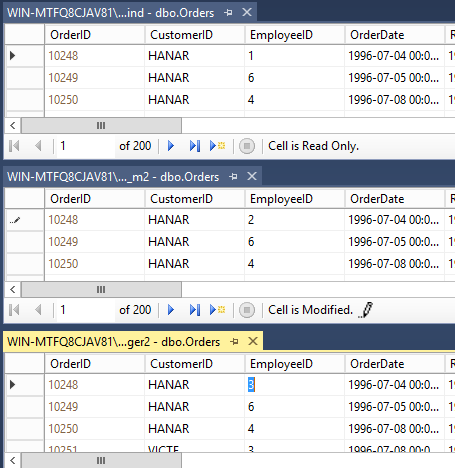
\includegraphics[width=0.75\linewidth,height=\textheight,keepaspectratio]{./images/img-048-052.png}

\begin{center}\rule{0.5\linewidth}{0.5pt}\end{center}

\subsection{Naplószállítás}\label{napluxf3szuxe1lluxedtuxe1s}

Míg a replikáció elsősorban üzleti folyamatok automatizálására alkalmas,
a naplószállítás egy adatbázis \textbf{katasztrófa utáni
helyreállítására} (disaster recovery) való felkészülésre lett tervezve:
egy pontos, általában csak olvasható másolatot hoz létre és tart
szinkronban --- ezt nevezik `meleg' tartalék adatbázisnak. A naplót az
elsődleges szerverről több másodlagos szerverre is el lehet küldeni.

A naplószállítás az adatbázis teljes biztonsági mentésével kezdődik,
amelyet visszaállítanak a másodlagos szerveren. Ezután a naplószállítás
három lépése a következő:

\begin{enumerate}
\def\labelenumi{\arabic{enumi}.}
\tightlist
\item
  Az elsődleges szerveren futó \textbf{biztonsági mentési feladat}
  (backup job) lementi az adatbázis tranzakciós naplójának új részét a
  helyi szerverre.
\end{enumerate}

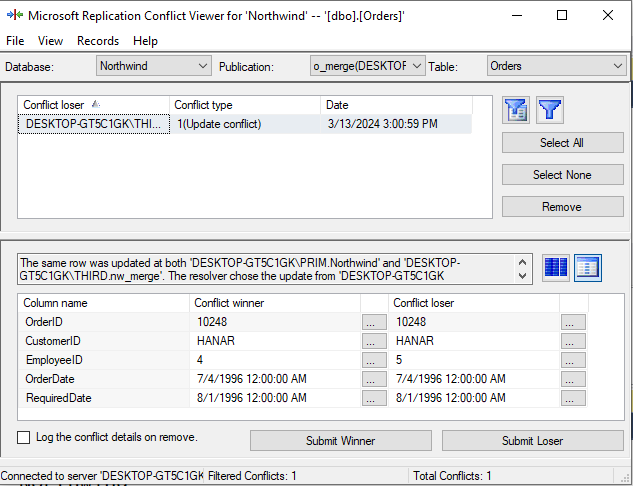
\includegraphics[width=0.75\linewidth,height=\textheight,keepaspectratio]{./images/img-049-053.png}

\begin{enumerate}
\def\labelenumi{\arabic{enumi}.}
\setcounter{enumi}{1}
\item
  A másodlagos szerveren futó \textbf{másolási feladat} (copy job)
  átmásolja a naplót egy konfigurálható célhelyre (pl. egy hálózati
  fájlszerverre).
\item
  A másodlagos szerveren futó \textbf{visszaállítási feladat} (restore
  job) visszaállítja a biztonsági mentést a másodlagos adatbázis(ok)ra.
\end{enumerate}

Egy figyelmeztető feladat is futhat, amely figyeli, hogy minden lépés a
vártnak megfelelően és időben elvégzésre kerül-e.

A feladatok ütemezésétől függően késleltetés van a két adatbázis között.
Ez a késleltetés kiaknázható, ha az elsődleges adatbázist véletlenül
módosítják.

\begin{quote}
\textbf{GYAKORLAT:} ebben a forgatókönyvben a Northwind adatbázisról
hozunk létre \textbf{`meleg biztonsági mentést'}. Ez azt jelenti, hogy
szerverhiba esetén a tartalék szerver (azaz a meleg biztonsági mentés)
néhány percen belül átveheti az éles szerver szerepét, anélkül hogy
hosszadalmas teljes biztonsági mentés visszaállítási eljárást kellene
elvégezni. Az elsődleges és másodlagos szerverek általában különböző
szervergépeken futnak, de a demóban ugyanazt a gépet és két
szerverpéldányt --- a Primary-t és a Secondary-t --- fogjuk használni. A
Third szerver monitorként fog működni.
\end{quote}

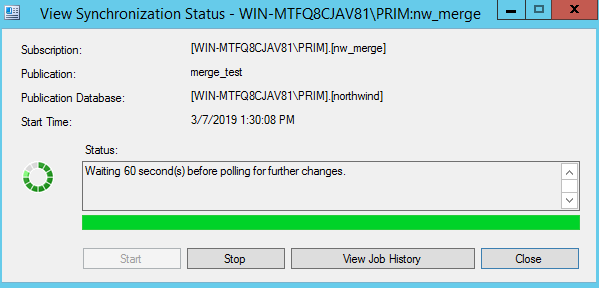
\includegraphics[width=0.75\linewidth,height=\textheight,keepaspectratio]{./images/img-049-054.png}

\begin{enumerate}
\def\labelenumi{\arabic{enumi}.}
\item
  Hozz létre egy mappát a naplók tárolásához és egy másikat, ahová a
  másolatot elhelyezed:

  \texttt{C:\textbackslash{}ship\textbackslash{}logs} és
  \texttt{C:\textbackslash{}ship\textbackslash{}dest}
\item
  Mindkét mappa megosztási beállításait
  (Tulajdonságok/Megosztás/Megosztás) állítsd be úgy, hogy mindenki
  számára elérhető legyen. Írd be az „Everyone'' nevet, és állítsd be az
  Olvasás/Írás jogosultságot.
\item
  Az elsődleges szerveren (PRIM) a Northwind adatbázis helyi menüjéből
  válaszd a Tulajdonságok lehetőséget, és ellenőrizd, hogy a Northwind
  adatbázis helyreállítási modellje Full értékre van-e állítva. Ez azt
  jelenti, hogy a napló inaktív részei nem törlődnek ellenőrzőpontnál.
\end{enumerate}

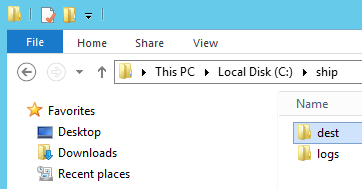
\includegraphics[width=0.75\linewidth,height=\textheight,keepaspectratio]{./images/img-050-055.png}

\begin{enumerate}
\def\labelenumi{\arabic{enumi}.}
\setcounter{enumi}{3}
\item
  A PRIM-en, a Northwind adatbázis Feladatok → Tranzakciós naplók
  szállítása paneljén engedélyezd az adatbázist szállításhoz, és válaszd
  a Biztonsági mentési beállítások lehetőséget. A biztonsági mentési
  mappa hálózati elérési útjaként add meg
  \texttt{\textbackslash{}\textbackslash{}WIN-MTFQ8CJAV81\textbackslash{}logs},
  a helyi mappa elérési útjaként pedig
  \texttt{C:\textbackslash{}ship\textbackslash{}logs} értéket.
\item
  Válaszd a Feladat szerkesztése lehetőséget, és állíts be egy
  ütemezést, amely percenként futtatja a feladatot. \emph{Megjegyzés: ez
  a beállítás csak bemutató célokra szól.}
\item
  Térj vissza az Adatbázis-tulajdonságok panelre, és kattints a
  Hozzáadás gombra a Másodlagos adatbázisok részben.
\item
  A Másodlagos adatbázis beállításai panelen add meg az
  \texttt{nw\_ship} nevet az új adatbázisnak. Fogadd el az inicializálás
  alapértelmezéseit. A Fájlok másolása fülön add meg
  \texttt{C:\textbackslash{}ship\textbackslash{}dest} értéket
  célmappaként. Az ütemezést állítsd percenkénti futásra.
  \emph{Megjegyzés: ez csak bemutató célokra szól.}
\item
  A Visszaállítás fülön válaszd a Készenléti módot (Standby mode) és a
  Felhasználók lecsatlakoztatása lehetőséget, majd állíts be percenkénti
  visszaállítási ütemezést. \emph{Megjegyzés: ez csak bemutató célokra
  szól.}
\end{enumerate}

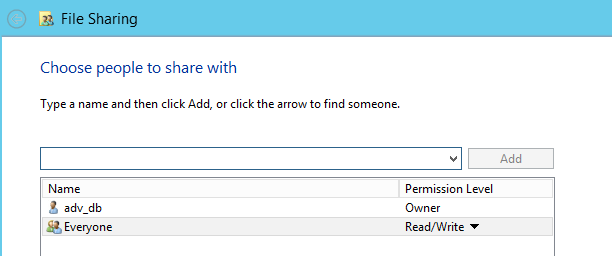
\includegraphics[width=0.75\linewidth,height=\textheight,keepaspectratio]{./images/img-051-056.png}

\begin{enumerate}
\def\labelenumi{\arabic{enumi}.}
\setcounter{enumi}{8}
\item
  Opcionálisan konfigurálhatod a THIRD szervert Monitor szerverként. A
  Monitor szerver az a példány, amely figyeli az elsődleges és
  másodlagos szervereket, és futtatja a naplószállítás figyelő
  feladatát. Ez a feladat hibát generál, ha a három folyamat (biztonsági
  mentés, másolás, visszaállítás) bármelyike nem sikerül megfelelően az
  előre beállított küszöbértékidőn belül (alapértelmezés: 45 perc).
  Tesztelési célokra használj rövidebb időszakot, például \textbf{2
  percet}. Az \texttt{sa} SQL Server megbízottat (principal) használd a
  figyelő feladat hitelesítésére az elsődleges és másodlagos példányok
  eléréséhez. Emellett két riasztás is automatikusan beállításra kerül a
  monitor példányon, az elsődleges és másodlagos példányok
  meghibásodásának esetére --- üres válasszal (amelyet a
  rendszergazdának kell konfigurálnia). Tipikus válasz az operátornak
  küldött e-mail értesítés.
\item
  Véglegesítsd és futtasd a konfigurációt.
\item
  Ellenőrizd a helyes működést mindkét adatbázishoz csatlakozva. Lehet,
  hogy 3 percet kell várnod, amíg a változások megjelennek a másodlagos
  adatbázisban. A naplószállítás aktuális állapotáról jelentést
  készíthetsz a Monitor szerver helyi menüjéből: Jelentések → Standard
  jelentések → Tranzakciós naplószállítás állapota.
\item
  Ellenőrizd a \texttt{logs} és \texttt{dest} mappák tartalmát.
  Percenként kell megjelennie a tranzakciós napló biztonsági
  mentéseinek.
\item
  Tiltsd le a naplószállítást a PRIM szerveren. Mivel a Secondary-n
  szállított adatbázis készenléti állapotban van, az eldobása előtt a
  következő parancsokat kell végrehajtanod (lásd alább). Alternatívaként
  az SSMS felületen is beállíthatod az adatbázist egyfelhasználós módba,
  visszaállíthatod recovery-vel, majd visszaállíthatod multi-user módba.
\end{enumerate}

\begin{Shaded}
\begin{Highlighting}[]
\KeywordTok{use} \KeywordTok{master}
\KeywordTok{alter} \KeywordTok{database}\NormalTok{ nw\_ship }\KeywordTok{set}\NormalTok{ single\_user }\KeywordTok{with} \KeywordTok{rollback} \KeywordTok{immediate}
\NormalTok{restore }\KeywordTok{database}\NormalTok{ nw\_ship }\KeywordTok{with} \KeywordTok{recovery}
\KeywordTok{alter} \KeywordTok{database}\NormalTok{ nw\_ship }\KeywordTok{set}\NormalTok{ multi\_user}
\end{Highlighting}
\end{Shaded}

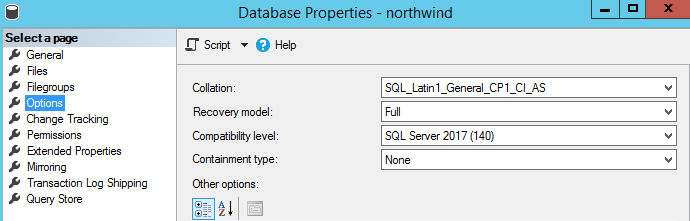
\includegraphics[width=0.75\linewidth,height=\textheight,keepaspectratio]{./images/img-051-057.png}

\begin{center}\rule{0.5\linewidth}{0.5pt}\end{center}

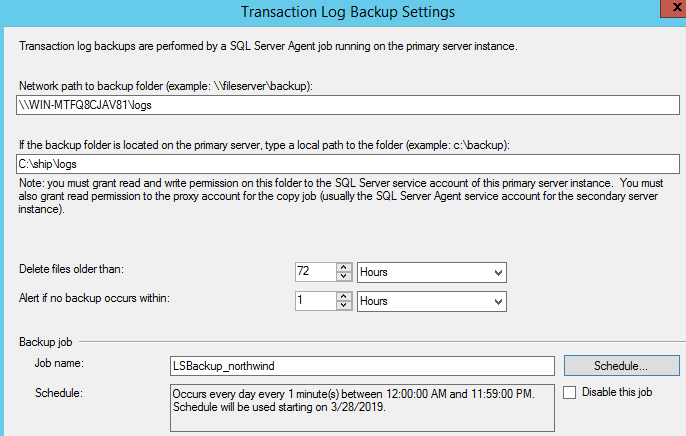
\includegraphics[width=0.75\linewidth,height=\textheight,keepaspectratio]{./images/img-052-058.png}

\subsection{Feladatátvételi
fürtök}\label{feladatuxe1tvuxe9teli-fuxfcrtuxf6k}

Definíció szerint: „A feladatátvételi fürtözés (FC) egy Windows Server
funkció, amely lehetővé teszi, hogy több kiszolgálót egyetlen hibatűrő
fürtté csoportosíts az alkalmazások és szolgáltatások --- például a
Microsoft SQL Server --- rendelkezésre állásának és méretezhetőségének
növelése érdekében.''\footnote{Lásd:
  https://docs.microsoft.com/hu-hu/windows-server/manage/windows-admin-center/use/manage-failover-clusters
  és
  https://docs.microsoft.com/hu-hu/windows-server/failover-clustering/failover-clustering-overview}
Egy FC-hez szerver típusú operációs rendszert igénylő, egynél több
szervergépen futó rendszerre van szükség. Ez az egyik oka annak, hogy
ezt a technológiát nem tudjuk bemutatni ebben a kurzusban.

Miután az FC-t beállítottuk, a fürttagokon futó SQL Server-példányok
konfigurálhatók egy Always On rendelkezésre állási csoportba. Egy ilyen
csoportban meghatározhatunk egy `rendelkezésre állási adatbázisok' nevű
adatbáziscsoportot, amelyek másolódnak a többi példányra, és együtt
hajtják végre a feladatátvételt. A feladatátvétel-támogatáson kívül
ilyen architektúra konfigurálható \emph{automatikus olvasási
terheléselosztásra} is a nagy terhelésű adatbázisoknál.

\begin{center}\rule{0.5\linewidth}{0.5pt}\end{center}

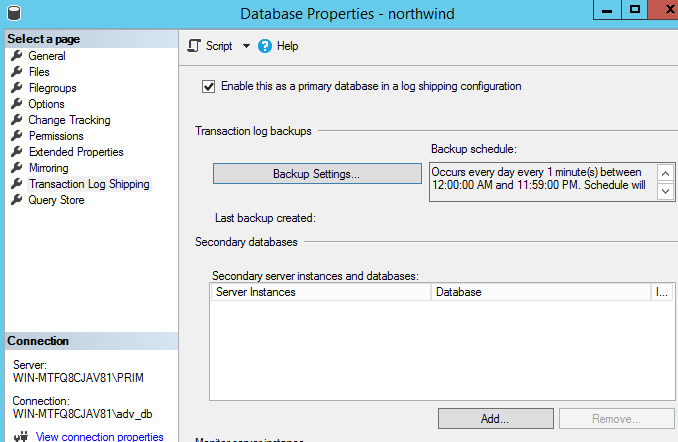
\includegraphics[width=0.75\linewidth,height=\textheight,keepaspectratio]{./images/img-053-059.png}

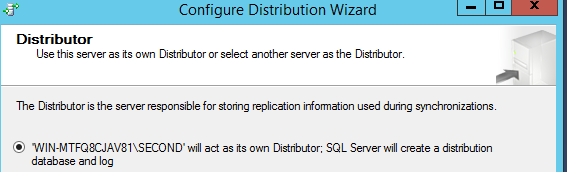
\includegraphics[width=0.75\linewidth,height=\textheight,keepaspectratio]{./images/img-036-033.png}

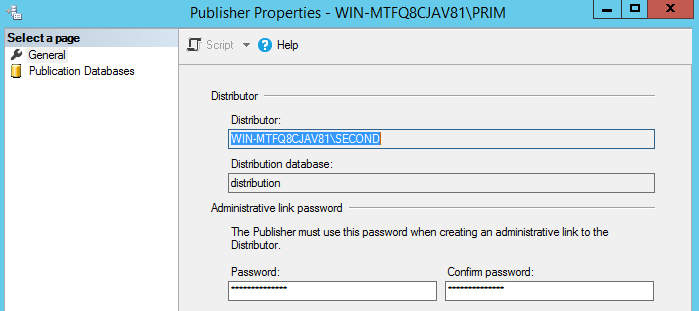
\includegraphics[width=0.75\linewidth,height=\textheight,keepaspectratio]{./images/img-041-041.png}

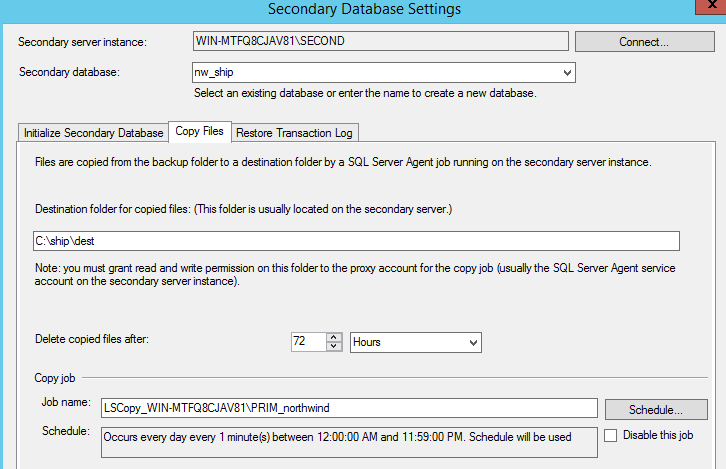
\includegraphics[width=0.75\linewidth,height=\textheight,keepaspectratio]{./images/img-054-060.png}

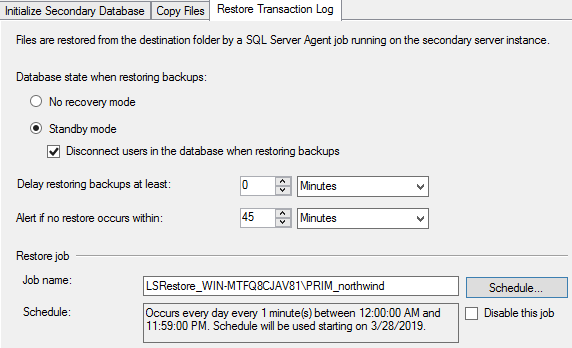
\includegraphics[width=0.75\linewidth,height=\textheight,keepaspectratio]{./images/img-055-061.png}

\section{4. Adatminőség és
törzsadat-menedzsment}\label{adatminux151suxe9g-uxe9s-tuxf6rzsadat-menedzsment}

Az adatok típusai egy vállalatnál:

\begin{itemize}
\tightlist
\item
  Tranzakciós (OLTP adatbázisokban)
\item
  Hierarchikus adatok (pl. taxonómiák)
\item
  Adattárházi adatok (data warehouse)
\item
  Félig strukturált (XML, JSON)
\item
  Strukturálatlan (e-mail, PDF, blogok)
\item
  Törzsadat (master data)
\item
  Metaadat (adat az adatról)
\end{itemize}

A magas adatminőség (DQ -- Data Quality) követelménye szigorúbb az
adatintegritásénál (pl. amikor elgépelt értékeket szeretnénk javítani).

Az adatminőség dimenziói:

\begin{itemize}
\tightlist
\item
  \textbf{Kemény dimenziók}

  \begin{itemize}
  \tightlist
  \item
    Teljesség (completeness) --- megvan-e minden adat?
  \item
    Pontosság (accuracy) --- helyesek-e az értékek?
  \item
    Konzisztencia (consistency) --- ellentmondanak-e az adatok egymásnak
    különböző rendszerekben?
  \end{itemize}
\item
  \textbf{Puha dimenziók:} a felhasználók szubjektív megítélése alapján,
  pl. bizalom.
\end{itemize}

Ha mind a puha, mind a kemény dimenziók értékelése gyenge,
Törzsadat-menedzsment (MDM -- Master Data Management) megoldást kell
alkalmazni. Az MDM-hez központi adattárolóra és \emph{adatkormányzásra}
(Data Governance) van szükség: ez az adatminőség megvalósításának
folyamata. Ehhez \emph{adatgondozók} (Data Stewards) kellenek: olyan
személyek, akik felelősek bizonyos adattípusok minőségéért --- például
egy gondozó felelős lehet az ügyféladatokért. \textbf{Az
MDM-technológiákat ez a tankönyv nem tárgyalja részletesen.}

Az adatminőség (DQ) tervezett vagy reaktív módon javítható, az utóbbi
kisebb vállalatoknál is alkalmazható. Egy DQ-megoldás sikerességét
nyomon követhetjük például azzal, hogy egy táblában a hibás vagy
ismeretlen rekordok száma hogyan csökken idővel.

\begin{quote}
\textbf{DEMO:} elemezd a táblák oszlopait teljesség, konzisztencia,
funkcionális függőség stb. szempontjából:
\end{quote}

\begin{Shaded}
\begin{Highlighting}[]
\KeywordTok{use}\NormalTok{ AdventureworksDW2019}

\CommentTok{{-}{-}vizsgáljuk, van{-}e funkcionális függés két oszlop között}
\KeywordTok{select}\NormalTok{ SalesReasonKey, SalesReasonName, SalesReasonReasonType }\KeywordTok{from}\NormalTok{ DimSalesReason}

\CommentTok{{-}{-}az adatok azt sugallják, hogy a SalesReasonReasonType oszlop függ}
\CommentTok{{-}{-}a SalesReasonName oszloptól, azaz az előbbi mindig megállapítható az utóbbiból}
\CommentTok{{-}{-}ellenőrizzük, hogy az adatok alátámasztják{-}e ezt a feltevést}

\KeywordTok{select}\NormalTok{ SalesReasonReasonType, }\FunctionTok{count}\NormalTok{(}\OperatorTok{*}\NormalTok{) }\KeywordTok{from}\NormalTok{ DimSalesReason }\KeywordTok{group} \KeywordTok{by}
\NormalTok{SalesReasonReasonType  }\CommentTok{{-}{-}3 csoport 4, 5 és 1 taggal}
\KeywordTok{select}\NormalTok{ SalesReasonName, }\FunctionTok{count}\NormalTok{(}\OperatorTok{*}\NormalTok{) }\KeywordTok{from}\NormalTok{ DimSalesReason }\KeywordTok{group} \KeywordTok{by}\NormalTok{ SalesReasonName  }\CommentTok{{-}{-}minden}
\CommentTok{{-}{-}csoportnak 1 tagja van {-}\textgreater{} jelölt kulcs}
\CommentTok{{-}{-}következtetés: a SalesReasonName valószínűleg a SalesReasonReasonType alkategóriája}

\CommentTok{{-}{-}funkcionális függés ellenőrzése}
\CommentTok{{-}{-}hogyan ellenőrizzük, hogy a CountryRegionCode funkcionálisan függ{-}e a StateProvinceCode{-}tól}
\KeywordTok{select} \OperatorTok{*} \KeywordTok{from}\NormalTok{ DimGeography}

\KeywordTok{select}\NormalTok{ StateProvinceCode, }\FunctionTok{count}\NormalTok{(}\OperatorTok{*}\NormalTok{) }\KeywordTok{from}\NormalTok{ DimGeography }\KeywordTok{group} \KeywordTok{by}\NormalTok{ StateProvinceCode }\CommentTok{{-}{-}71}
\KeywordTok{select}\NormalTok{ StateProvinceCode, }\FunctionTok{count}\NormalTok{(}\OperatorTok{*}\NormalTok{) }\KeywordTok{from}\NormalTok{ DimGeography }\KeywordTok{group} \KeywordTok{by}
\NormalTok{StateProvinceCode,CountryRegionCode  }\CommentTok{{-}{-}71}
\CommentTok{{-}{-}71=71, tehát egy StateProvinceCode mindig ugyanazt a CountryRegionCode{-}ot kapja}
\CommentTok{{-}{-}nagy valószínűséggel funkcionális függés van a két mező között}
\KeywordTok{select}\NormalTok{ color, }\FunctionTok{count}\NormalTok{(}\OperatorTok{*}\NormalTok{) }\KeywordTok{from}\NormalTok{ dimproduct }\KeywordTok{group} \KeywordTok{by}\NormalTok{ color }\CommentTok{{-}{-}10}
\KeywordTok{select}\NormalTok{ ProductLine, }\FunctionTok{count}\NormalTok{(}\OperatorTok{*}\NormalTok{) }\KeywordTok{from}\NormalTok{ dimproduct }\KeywordTok{group} \KeywordTok{by}\NormalTok{ productline }\CommentTok{{-}{-}5}
\KeywordTok{select}\NormalTok{ ProductLine, }\FunctionTok{count}\NormalTok{(}\OperatorTok{*}\NormalTok{) }\KeywordTok{from}\NormalTok{ dimproduct }\KeywordTok{group} \KeywordTok{by}\NormalTok{ productline, color }\CommentTok{{-}{-}27 \textgreater{} 5, 27}
\OperatorTok{\textgreater{}} \DecValTok{10}
\CommentTok{{-}{-}nincs funkcionális függés a két mező között}
\end{Highlighting}
\end{Shaded}

\begin{quote}
\textbf{GYAKORLAT:} elemezd a DimCustomer és DimEmployee táblák
oszlopait teljesség és funkcionális függőség szempontjából. DimCustomer:
Education↔Occupation, DimEmployee: SalesTerritory↔Gender.
\end{quote}

Egy de facto funkcionális függőség az üzleti terület modellezetlen, de
létező üzleti szabályából is eredhet. Az ilyen rejtett kapcsolat
megsértheti a 3NF-struktúrát egy táblán belüli tranzitív függőség révén,
és \textbf{redundanciához és inkonzisztenciához} vezethet. Ezért érdeke
a vállalatnak, hogy adatelemzéssel felderítse az ilyen összefüggéseket.

\textbf{Példa:} az alkalmazottainknak van munkaköri kódjuk (pl. kutató,
menedzser, műszaki, titkár) és iskolai végzettség-kódjuk (pl. általános
iskola, középiskola, PhD). Elképzelhető, hogy a vállalatnál olyan
szabályzat él, amely csak egy bizonyos végzettséget engedélyez egy adott
munkakörhöz --- ezzel de facto funkcionális függőséget hozva létre a két
mező között. A végzettség a munkakörtől függhet.

\begin{center}\rule{0.5\linewidth}{0.5pt}\end{center}

\subsection{Adatprofil-elemzés}\label{adatprofil-elemzuxe9s}

Az adatprofil-elemzés (Data Profiling) célja, hogy automatikusan
megtalálja egy oszlop statisztikai és adatminőséggel kapcsolatos
jellemzőit:

\begin{itemize}
\tightlist
\item
  Funkcionális függőségek, jelölt kulcsok és potenciális idegen kulcsok
  azonosítása (lásd fentebb)
\item
  Oszlopérték-eloszlások és egyéb statisztikák kiszámítása
\item
  Null-arány és hosszeloszlás mérése szöveges típusoknál
\item
  \emph{De facto} oszlopminták levezetése reguláris kifejezésekként az
  értékekből --- ezek \emph{tartományszabályokként} (domain rules)
  használhatók (lásd később)
\end{itemize}

MS SQL Serverben az adatprofil-elemzés az Integration Services Data
Profiling Task segítségével végezhető el, amely az eredményeket
XML-fájlba menti (ebben a tankönyvben nem részletezzük).\footnote{Lásd:
  https://docs.microsoft.com/en-us/sql/integration-services/control-flow/data-profiling-task-and-viewer}

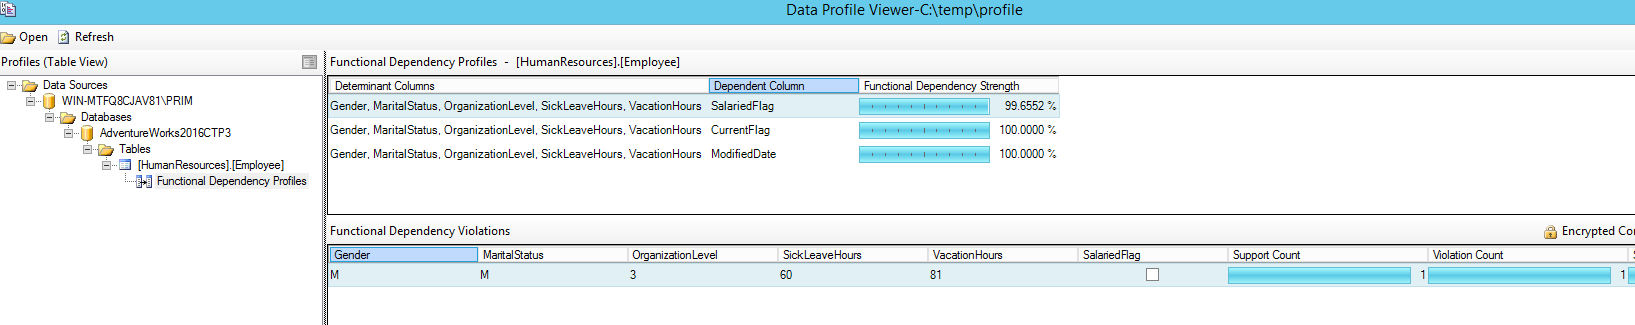
\includegraphics[width=0.75\linewidth,height=\textheight,keepaspectratio]{./images/img-058-062.png}

\begin{center}\rule{0.5\linewidth}{0.5pt}\end{center}

\subsection{SQL Server Data Quality
Services}\label{sql-server-data-quality-services}

A DQS (Data Quality Services) szolgáltatás felelős a referenciaadatok
tisztításáért, profilozásáért és egyeztetéséért. A DQS szerver a DQS
motort és a DQS adatbázisokat foglalja magában:

\begin{itemize}
\tightlist
\item
  \textbf{DQS\_MAIN:} a DQS motort megvalósító tárolt eljárások,
  valamint tudásbázisok (pl. US -- Last Name tudásbázis,
  referenciaadatok: pl. magyarországi városok). Szerepkörök a DQS\_MAIN
  adatbázisban: \texttt{dqs\_administrator}, \texttt{dqs\_kb\_editor},
  \texttt{dqs\_kb\_operator} (különböző felhasználókhoz rendelhetők)
\item
  \textbf{DQS\_PROJECTS:} a tisztítási és egyeztetési projektekhez
  szükséges adatok
\item
  \textbf{DQS\_STAGING\_DATA:} ideiglenes tároló a tisztítandó adatokhoz
  és a tisztítás eredményéhez
\end{itemize}

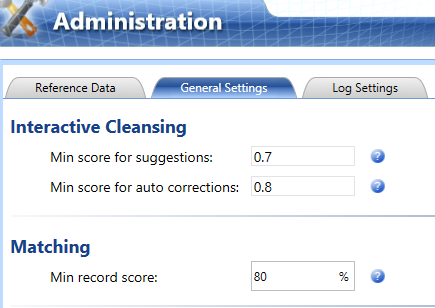
\includegraphics[width=0.75\linewidth,height=\textheight,keepaspectratio]{./images/img-059-063.png}

Egy Data Quality kliens által elvégzendő feladatok: tudásbázisok
kezelése, tisztítási/egyeztetési projektek végrehajtása, DQS
adminisztrálása. Kliensimplementációk:

\begin{itemize}
\tightlist
\item
  Egy SQL Server Integration Services `DQS Cleansing transformation'
  komponens elvégezheti a tisztítást egy SSIS-csomag adatfolyamában
\item
  SQL Server 2017 Data Quality Client (DQC), egy asztali alkalmazás
\end{itemize}

\subsubsection{Adattisztítási
projektek}\label{adattisztuxedtuxe1si-projektek}

A DQS-projektek két fajtája:

\begin{itemize}
\tightlist
\item
  \textbf{Alapvető adattisztítás} (Basic data cleansing): az egyedi
  mezőértékek javítása a cél. Ezt a projekttípust mutatjuk be ezen a
  kurzuson.
\item
  \textbf{Azonosság-leképezés és deduplikáció} (Identity mapping and
  de-duplicating) egyeztetési szabályok alapján: a cél az esetlegesen
  duplikált rekordok --- vagyis entitások --- azonosítása és
  eltávolítása. Az egyeztetési szabályt tudásbázis szinten kell
  definiálni, az adattudományban elterjedt távolságmértékek
  alkalmazásával. Ezt a projekttípust nem mutatjuk be ezen a kurzuson.
\end{itemize}

Mindkét típus a DQS\_MAIN adatbázisban már telepített tudásbázison (KB)
alapul, és ezeket a paramétereket használja:

\begin{itemize}
\tightlist
\item
  \textbf{Tisztítás:} a Javaslat minimális pontszáma (Min Score for
  Suggestions) a javaslat generálásához szükséges minimális hasonlóságot
  adja meg. Ennek \emph{kisebbnek} kell lennie, mint az Automatikus
  javítás minimális pontszáma (Min Score for Auto Correction).
\item
  \textbf{Egyeztetés (deduplikáció):} küszöbérték az egyeztetési
  szabályhoz. Ez a rekordok hasonlóságának mértéke.
\end{itemize}

Egy DQS \textbf{tudásbázis} (Knowledge Base, KB) több
\textbf{tartományt} (domain) tartalmazhat, vagyis a tisztításhoz
használt referencia-értékkészleteket. Egy tartományt a következő
összetevők határoznak meg:

\begin{itemize}
\tightlist
\item
  \textbf{Név és adattípus}, pl. string
\item
  Normalizálási beállítások, mint nagybetűssé alakítás, üres karakterek
  eltávolítása, formázás és helyesírás-ellenőrzés
\item
  Referenciaadatok, amelyek tárolhatók a DQS\_MAIN adatbázisban, vagy
  alternatívaként külső szolgáltatás is nyújthatja őket

  \begin{itemize}
  \tightlist
  \item
    A referencia-értékeket \textbf{tartományértékeknek} (domain values
    -- referenciaértékek) hívják. Egy tartományérték egy olyan sor,
    amely tartalmaz egy \textbf{főértéket} (leading value --
    alapértelmezett érték) és annak szinonimáinak listáját
  \end{itemize}
\item
  \textbf{Tartományszabályok} (Domain rules), hasonlóak a
  CHECK-megszorításokhoz
\item
  \textbf{Szövegrész-alapú kapcsolatok} (Term based relations), amelyek
  az érték egy részére vonatkoznak, pl.
  \texttt{\textquotesingle{}\%Ltd.\%\textquotesingle{}} →
  \texttt{\textquotesingle{}\%Limited\ Company\%\textquotesingle{}}
\end{itemize}

\textbf{Összetett tartományok} (Composite domains) szemantikailag
összetartozó mezőkből hozhatók létre, pl. egy több oszlopban tárolt cím
város, utca stb. részeiből.

A PRIM szerveren a DQS\_MAIN-ben már telepítve vannak alapértelmezett
tudásbázisok, pl. Country/Region, US-Counties, US-Last names. Saját
tudásbázist is létrehozhatunk.

\begin{quote}
\textbf{DEMO:} megtisztítjuk egy tábla vezetékneveit az alapértelmezett
KB segítségével.
\end{quote}

Indítsd el a DQC-t, és add meg a szervernevet:
\texttt{WIN-MTFQ8CJAV81\textbackslash{}PRIM}.

\begin{itemize}
\tightlist
\item
  Az Administration → Configuration → General settings panelen tekintsd
  át a Min Score for Suggestions és Min Score for Auto Correction
  beállításokat. Ezeket kísérletezéssel lehet finomhangolni.
\item
  A Knowledge base management panelen tekintsd át az előre telepített
  tudásbázisokat.
\item
  Hozz létre egy új adattisztítási projektet \texttt{Lastnames} névvel.
\item
  Válaszd ki a KB-t: DQS Data, és a US\_Last Name tartományt. A
  tevékenység legyen Cleansing (Tisztítás).
\item
  A Map oldalon válaszd ki az AdventureworksDW2019 adatbázist, a
  DimCustomer táblát és a Lastname mezőt, és rendeld hozzá a US\_Last
  Name tartományhoz.
\item
  Indítsd el a tisztítási folyamatot. Mivel a DimCustomer táblában több
  mint 18 000 vezetéknevet kell megtisztítani, az előfeldolgozás kb. 5
  percig, a tisztítás kb. 30 másodpercig tart.
  \textbf{FIGYELEM:}\footnote{Ha a `Parallel processing task failed'
    hibát kapod az előfeldolgozás során, ellenőrizd a
    DQServerLog.DQS\_MAIN.log fájlt a példány Log könyvtárában. A hiba:
    \emph{`The DELETE statement conflicted with the REFERENCE constraint
    ``B\_INDEX\_LEXICON\_EXTENSION\_B\_INDEX\_LEXICON\_FK''. The
    conflict occurred in database ``DQS\_PROJECTS'', table
    ``DQProject1000001.B\_INDEX\_LEXICON\_EXTENSION'', column
    'TERM\_ID'\,'}. Az SSMS Modify keys paneljén állítsd a
    B\_INDEX\_LEXICON\_EXTENSION\_B\_INDEX\_LEXICON\_FK idegen
    kulcs-megszorítás On Delete műveletét CASCADE értékre.}
\item
  Ellenőrizd a kemény dimenziókat: Teljesség (100\%) és Pontosság
  (98\%). A tisztítás után egy érték a következő állapotok egyikébe
  kerülhet:

  \begin{itemize}
  \tightlist
  \item
    \textbf{Helyes} (Correct): megtalálható a tartományértékek között
  \item
    \textbf{Javított} (Corrected): automatikusan módosítva egy
    tartományértékre, mert a hasonlóság meghaladta az Automatikus
    javítás minimális pontszámát
  \item
    \textbf{Javasolt} (Suggested): új értéket csak javasol a rendszer,
    mert a hasonlóság meghaladta a Javaslat minimális pontszámát
  \item
    \textbf{Új} (New): a tartományértékek között nem található hasonló
    érték, de az érték megfelel a tartományszabályoknak
  \item
    \textbf{Érvénytelen} (Invalid): egy új érték, amely ellentmond a
    tartományszabályoknak
  \end{itemize}
\item
  A fenti Min Score beállításokkal a folyamat néhány esetet talál, ahol
  javítást javasol, és 3 esetet, ahol automatikus javítást végzett. 328
  nevet helyesen talált meg a KB-ban.
\item
  Próbálj meg jóváhagyni egy javasolt módosítást → a sor átkerül a
  Javított panelre.
\item
  Végül mentsd el a megtisztított táblát a LastNameSource és
  LastNameOutput oszlopokkal az eredeti adatbázisba, és dolgozd fel
  T-SQL parancsokkal.
\end{itemize}

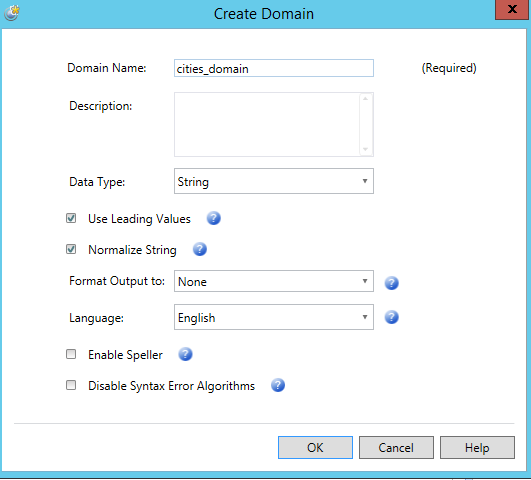
\includegraphics[width=0.75\linewidth,height=\textheight,keepaspectratio]{./images/img-062-064.png}

\begin{quote}
\textbf{GYAKORLAT:} tisztítsd meg az
AdventureworksDW2019.DimGeography.EnglishCountryRegionName mezőt a
Country/Region tartomány segítségével. Próbáld meg újra, miután
hozzáadtál egy elírt országnevet a táblához (Austrila).
\end{quote}

\subsubsection{Saját tudásbázis
létrehozása}\label{sajuxe1t-tuduxe1sbuxe1zis-luxe9trehozuxe1sa}

Egy táblamező meglévő értékkészletét felhasználhatjuk saját KB
összeállításához. A lépések:

\begin{enumerate}
\def\labelenumi{\arabic{enumi}.}
\tightlist
\item
  Automatikus tudásfelderítés az adatminta alapján
\item
  Manuális tartománykezelés és -konfiguráció
\end{enumerate}

\begin{quote}
\textbf{DEMO:} létrehozunk egy KB-t.
\end{quote}

\begin{itemize}
\tightlist
\item
  Hozz létre egy új nézetet a DQS\_STAGING\_DATA adatbázisban:
\end{itemize}

\begin{Shaded}
\begin{Highlighting}[]
\KeywordTok{use}\NormalTok{ DQS\_STAGING\_DATA}
\NormalTok{go}
\KeywordTok{create} \KeywordTok{view}\NormalTok{ vi\_places }\KeywordTok{as}
\KeywordTok{select} \KeywordTok{distinct}\NormalTok{ City, StateProvinceName StateProvince, EnglishCountryRegionName}
\NormalTok{CountryRegion}
\KeywordTok{from}\NormalTok{ AdventureworksDW2019.dbo.DimGeography}
\NormalTok{go}
\end{Highlighting}
\end{Shaded}

\begin{itemize}
\item
  Indítsd el a DQS klienst, és hozz létre egy új, \texttt{places} nevű
  KB-t.
\item
  Válaszd a Knowledge discovery lehetőséget, állítsd be forrásként a
  \texttt{vi\_places} nézetet, és hozz létre két tartományt:
  \texttt{cities\_domain} és \texttt{countryregion\_domain}, a
  \texttt{vi\_places} nézet azonos nevű mezőit használva.
\item
  Indítsd el a felderítést.
\item
  A Muehlheim-bejegyzésnél állítsd a típust \textbf{Error} értékre, és a
  `Correct to' mezőbe írd be manuálisan: \texttt{Mühlheim}, \emph{majd
  nyomj Entert}.
\item
  Válaszd ki az új KB-t a főmenüből, és a helyi menüből válaszd a Domain
  management lehetőséget.
\item
  Adj hozzá manuálisan egy új tartományt \texttt{birth\_domain} névvel,
  egy egyszerű tartományszabállyal:
\end{itemize}

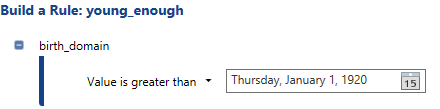
\includegraphics[width=0.75\linewidth,height=\textheight,keepaspectratio]{./images/img-062-065.png}

\textbf{Build a Rule: young\_enough}

\begin{itemize}
\item
  \texttt{birth\_domain} → Érték nagyobb mint: 1920. január 1.,
  csütörtök
\item
  Tedd közzé a KB-t.
\item
  Válaszd ki az új KB-t kezelésre, és exportáld egy \texttt{places.dqs}
  nevű fájlba.
\item
  Hozz létre egy \texttt{test\_customer} nevű táblát a
  DQS\_STAGING\_DATA adatbázisban a DimCustomer és DimGeography táblák
  GeographyKey oszlopon összekapcsolt adataiból.
\item
  Módosítsd az első ügyfél születési dátumát 1925-01-02-re, városát
  Muehlheimre. A második ügyfél városát változtasd Piripócsra.
\item
  Az új `places' KB segítségével tisztítsd meg a \texttt{test\_customer}
  táblát, és tekintsd meg az eredményeket.
\end{itemize}

\begin{quote}
\textbf{GYAKORLAT:} építs KB-t a DimProduct tábla ProductName mezőjét
felhasználva, és mutasd be alkalmazását a fentiek szerint.
\end{quote}

Ingyenes, független eszközök is elérhetők adattisztításhoz és
törzsadat-menedzsmenthez, pl. https://openrefine.org/

\begin{center}\rule{0.5\linewidth}{0.5pt}\end{center}

\section{5. Oszloptár és
particionálás}\label{oszloptuxe1r-uxe9s-particionuxe1luxe1s}

\subsection{Oszloptár (Columnstore)}\label{oszloptuxe1r-columnstore}

Az oszloptár (columnstore) egy alternatív módszer a relációs adatok
tárolására. \textbf{Sok mezőt tartalmazó, nagy adattárházi táblákhoz és
ritkán változó adatokhoz} ajánlott. Az adatlapokon (page-eken) egy
rekord mezői nem együtt tárolódnak; ehelyett minden mezőt önállóan
tárolnak, és a rekord értékei logikai rekordazonosítók alapján
kapcsolódnak össze.\footnote{Lásd:
  https://learn.microsoft.com/en-us/sql/relational-databases/indexes/columnstore-indexes-overview?view=sql-server-ver16}
Gyorsaságát az alacsony I/O-műveletszámnak (blokkos olvasásnak)
köszönheti, amely az alábbi tényezőkből ered:

\begin{itemize}
\tightlist
\item
  A lapok tömörítése\footnote{Lásd:
    https://learn.microsoft.com/en-us/sql/relational-databases/data-compression/data-compression?view=sql-server-ver16}
  (kisebb méret → kevesebb lap), valamint az a tény, hogy a lekérdezések
  általában nem igénylik az egész rekord olvasását, csak néhány mezőét
\item
  Ez különösen szembetűnő, ha a tábla nagyon sok mezőt tartalmaz --- ami
  az adattárházakra jellemző.
\end{itemize}

Tömörítési típusok:

\begin{itemize}
\tightlist
\item
  \textbf{Sor-alapú tömörítés} (Row compression): a rögzített hosszúságú
  adattípusokat változó hosszúságú adattal helyettesíti, pl. egy 4
  bájtos integer mező az aktuális értéktől függően 1 bájtban is
  tárolható. OLTP alkalmazásokban alkalmazható.
\item
  \textbf{Lap-alapú tömörítés} (Page compression): teljes lapokat
  tömörít; adattárházi alkalmazásokra vagy ritkán frissített OLTP
  alkalmazásokra inkább alkalmas. Különösen hatékony, ha egy mező
  értékei nagyon hasonlóak --- ezeket \emph{alacsony kardinalitású} (low
  cardinality, azaz kevés különböző értékkel rendelkező) mezőknek
  nevezzük.
\end{itemize}

Az alábbiakban oszloptárat és lap-alapú tömörítést mutatunk be SQL
Serveren --- a Postgres ingyenes kiadása jelenleg nem támogatja a
tömörítést.

\begin{Shaded}
\begin{Highlighting}[]
\KeywordTok{use}\NormalTok{ AdventureWorksDW2016\_ext}

\CommentTok{/*}
\CommentTok{{-}{-}BTREE tábla létrehozása}
\CommentTok{select * into FactResellerSalesXL\_BTREE from FactResellerSalesXL\_CCI {-}{-}2min 30s}
\CommentTok{alter table FactResellerSalesXL\_BTREE alter column SalesOrderLineNumber tinyint not null}
\CommentTok{alter table FactResellerSalesXL\_BTREE alter column SalesOrderNumber nvarchar(20) not null}
\CommentTok{alter table FactResellerSalesXL\_BTREE add constraint c1 primary key}
\CommentTok{(SalesOrderLineNumber, SalesOrderNumber) {-}{-}2min}
\CommentTok{*/}

\CommentTok{{-}{-}SZERVER ÚJRAINDÍTÁSA}
\KeywordTok{set} \KeywordTok{statistics} \DataTypeTok{time} \KeywordTok{on}
\KeywordTok{set} \KeywordTok{statistics}\NormalTok{ io }\KeywordTok{on}
\NormalTok{go}
\KeywordTok{select} \FunctionTok{count}\NormalTok{(}\OperatorTok{*}\NormalTok{) }\KeywordTok{from}\NormalTok{ FactResellerSalesXL\_BTREE  }\CommentTok{{-}{-}11669638}
\KeywordTok{exec}\NormalTok{ sp\_spaceused }\StringTok{\textquotesingle{}dbo.FactResellerSalesXL\_BTREE\textquotesingle{}}\NormalTok{, @updateusage }\OperatorTok{=} \StringTok{\textquotesingle{}TRUE\textquotesingle{}}
\CommentTok{{-}{-}adat: 2523168 KB, index: 9776 KB}

\KeywordTok{select} \FunctionTok{count}\NormalTok{(}\OperatorTok{*}\NormalTok{) }\KeywordTok{from}\NormalTok{ FactResellerSalesXL\_PageCompressed  }\CommentTok{{-}{-}11669638}
\KeywordTok{exec}\NormalTok{ sp\_spaceused }\StringTok{\textquotesingle{}dbo.FactResellerSalesXL\_PageCompressed\textquotesingle{}}\NormalTok{, @updateusage }\OperatorTok{=} \StringTok{\textquotesingle{}TRUE\textquotesingle{}}
\CommentTok{{-}{-}adat: 695624 KB, index: 2344 KB}

\KeywordTok{select} \FunctionTok{count}\NormalTok{(}\OperatorTok{*}\NormalTok{) }\KeywordTok{from}\NormalTok{ FactResellerSalesXL\_CCI  }\CommentTok{{-}{-}11669638}
\KeywordTok{exec}\NormalTok{ sp\_spaceused }\StringTok{\textquotesingle{}dbo.FactResellerSalesXL\_CCI\textquotesingle{}}\NormalTok{, @updateusage }\OperatorTok{=} \StringTok{\textquotesingle{}TRUE\textquotesingle{}}
\CommentTok{{-}{-}adat: 525344 KB, index: 157624 KB}

\NormalTok{go}
\NormalTok{dbcc freeproccache }\CommentTok{{-}{-}}

\NormalTok{dbcc dropcleanbuffers }\CommentTok{{-}{-} adatpuffer ürítése}

\CommentTok{{-}{-}B{-}TREE}
\CommentTok{{-}{-}========}
\KeywordTok{select}\NormalTok{ b.SalesTerritoryRegion}
\NormalTok{  ,FirstName }\OperatorTok{+} \StringTok{\textquotesingle{} \textquotesingle{}} \OperatorTok{+}\NormalTok{ LastName }\KeywordTok{as}\NormalTok{ FullName}
\NormalTok{  ,}\FunctionTok{count}\NormalTok{(SalesOrderNumber) }\KeywordTok{as}\NormalTok{ NumSales}
\NormalTok{  ,}\FunctionTok{sum}\NormalTok{(SalesAmount) }\KeywordTok{as}\NormalTok{ TotalSalesAmt}
\NormalTok{  ,}\FunctionTok{Avg}\NormalTok{(SalesAmount) }\KeywordTok{as}\NormalTok{ AvgSalesAmt}
\NormalTok{  ,}\FunctionTok{count}\NormalTok{(}\KeywordTok{distinct}\NormalTok{ SalesOrderNumber) }\KeywordTok{as}\NormalTok{ NumOrders}
\NormalTok{  ,}\FunctionTok{count}\NormalTok{(}\KeywordTok{distinct}\NormalTok{ ResellerKey) }\KeywordTok{as}\NormalTok{ NumResellers}
\KeywordTok{from}\NormalTok{ FactResellerSalesXL\_BTREE a}
\KeywordTok{inner} \KeywordTok{join}\NormalTok{ DimSalesTerritory b }\KeywordTok{on}\NormalTok{ b.SalesTerritoryKey }\OperatorTok{=}\NormalTok{ a.SalesTerritoryKey}
\KeywordTok{inner} \KeywordTok{join}\NormalTok{ DimEmployee d }\KeywordTok{on}\NormalTok{ d.Employeekey }\OperatorTok{=}\NormalTok{ a.EmployeeKey}
\KeywordTok{inner} \KeywordTok{join}\NormalTok{ DimDate c }\KeywordTok{on}\NormalTok{ c.DateKey }\OperatorTok{=}\NormalTok{ a.OrderDateKey}
\KeywordTok{where}\NormalTok{ b.SalesTerritoryKey }\OperatorTok{=} \DecValTok{3} \KeywordTok{and}\NormalTok{ c.FullDateAlternateKey }\KeywordTok{between} \StringTok{\textquotesingle{}1/1/2006\textquotesingle{}} \KeywordTok{and}
\StringTok{\textquotesingle{}1/1/2010\textquotesingle{}}
\KeywordTok{group} \KeywordTok{by}\NormalTok{ b.SalesTerritoryRegion,d.EmployeeKey,d.FirstName,d.LastName,c.CalendarYear}
\CommentTok{{-}{-}CPU idő = 3949 ms, eltelt idő = 9568 ms}

\CommentTok{{-}{-}DATA\_COMPRESSION = PAGE}
\CommentTok{{-}{-}==================================}
\NormalTok{go}
\KeywordTok{select}\NormalTok{ b.SalesTerritoryRegion}
\NormalTok{  ,FirstName }\OperatorTok{+} \StringTok{\textquotesingle{} \textquotesingle{}} \OperatorTok{+}\NormalTok{ LastName }\KeywordTok{as}\NormalTok{ FullName}
\NormalTok{  ,}\FunctionTok{count}\NormalTok{(SalesOrderNumber) }\KeywordTok{as}\NormalTok{ NumSales}
\NormalTok{  ,}\FunctionTok{sum}\NormalTok{(SalesAmount) }\KeywordTok{as}\NormalTok{ TotalSalesAmt}
\NormalTok{  ,}\FunctionTok{Avg}\NormalTok{(SalesAmount) }\KeywordTok{as}\NormalTok{ AvgSalesAmt}
\NormalTok{  ,}\FunctionTok{count}\NormalTok{(}\KeywordTok{distinct}\NormalTok{ SalesOrderNumber) }\KeywordTok{as}\NormalTok{ NumOrders}
\NormalTok{  ,}\FunctionTok{count}\NormalTok{(}\KeywordTok{distinct}\NormalTok{ ResellerKey) }\KeywordTok{as}\NormalTok{ NumResellers}
\KeywordTok{from}\NormalTok{ FactResellerSalesXL\_PageCompressed a}
\KeywordTok{inner} \KeywordTok{join}\NormalTok{ DimSalesTerritory b }\KeywordTok{on}\NormalTok{ b.SalesTerritoryKey }\OperatorTok{=}\NormalTok{ a.SalesTerritoryKey}
\KeywordTok{inner} \KeywordTok{join}\NormalTok{ DimEmployee d }\KeywordTok{on}\NormalTok{ d.Employeekey }\OperatorTok{=}\NormalTok{ a.EmployeeKey}
\KeywordTok{inner} \KeywordTok{join}\NormalTok{ DimDate c }\KeywordTok{on}\NormalTok{ c.DateKey }\OperatorTok{=}\NormalTok{ a.OrderDateKey}
\KeywordTok{where}\NormalTok{ b.SalesTerritoryKey }\OperatorTok{=} \DecValTok{3}
  \KeywordTok{and}\NormalTok{ c.FullDateAlternateKey }\KeywordTok{between} \StringTok{\textquotesingle{}1/1/2006\textquotesingle{}} \KeywordTok{and} \StringTok{\textquotesingle{}1/1/2010\textquotesingle{}}
\KeywordTok{group} \KeywordTok{by}\NormalTok{ b.SalesTerritoryRegion,d.EmployeeKey,d.FirstName,d.LastName,c.CalendarYear}
\NormalTok{GO  }\CommentTok{{-}{-} CPU idő = 3264 ms, eltelt idő = 3776 ms.}

\CommentTok{{-}{-}oszloptár lap{-}alapú tömörítéssel}
\CommentTok{{-}{-}create clustered columnstore index [IndFactResellerSalesXL\_CCI] on}
\CommentTok{{-}{-}[dbo].[FactResellerSalesXL\_CCI]}
\CommentTok{{-}{-}with (drop\_existing = off, compression\_delay = 0, data\_compression = columnstore) on}
\CommentTok{{-}{-}[primary]}
\CommentTok{{-}{-}================================}
\KeywordTok{select}\NormalTok{ b.SalesTerritoryRegion}
\NormalTok{  ,FirstName }\OperatorTok{+} \StringTok{\textquotesingle{} \textquotesingle{}} \OperatorTok{+}\NormalTok{ LastName }\KeywordTok{as}\NormalTok{ FullName}
\NormalTok{  ,}\FunctionTok{count}\NormalTok{(SalesOrderNumber) }\KeywordTok{as}\NormalTok{ NumSales}
\NormalTok{  ,}\FunctionTok{sum}\NormalTok{(SalesAmount) }\KeywordTok{as}\NormalTok{ TotalSalesAmt}
\NormalTok{  ,}\FunctionTok{Avg}\NormalTok{(SalesAmount) }\KeywordTok{as}\NormalTok{ AvgSalesAmt}
\NormalTok{  ,}\FunctionTok{count}\NormalTok{(}\KeywordTok{distinct}\NormalTok{ SalesOrderNumber) }\KeywordTok{as}\NormalTok{ NumOrders}
\NormalTok{  ,}\FunctionTok{count}\NormalTok{(}\KeywordTok{distinct}\NormalTok{ ResellerKey) }\KeywordTok{as}\NormalTok{ NumResellers}
\KeywordTok{from}\NormalTok{ FactResellerSalesXL\_CCI a}
\KeywordTok{inner} \KeywordTok{join}\NormalTok{ DimSalesTerritory b }\KeywordTok{on}\NormalTok{ b.SalesTerritoryKey }\OperatorTok{=}\NormalTok{ a.SalesTerritoryKey}
\KeywordTok{inner} \KeywordTok{join}\NormalTok{ DimEmployee d }\KeywordTok{on}\NormalTok{ d.Employeekey }\OperatorTok{=}\NormalTok{ a.EmployeeKey}
\KeywordTok{inner} \KeywordTok{join}\NormalTok{ DimDate c }\KeywordTok{on}\NormalTok{ c.DateKey }\OperatorTok{=}\NormalTok{ a.OrderDateKey}
\KeywordTok{where}\NormalTok{ b.SalesTerritoryKey }\OperatorTok{=} \DecValTok{3}
  \KeywordTok{and}\NormalTok{ c.FullDateAlternateKey }\KeywordTok{between} \StringTok{\textquotesingle{}1/1/2006\textquotesingle{}} \KeywordTok{and} \StringTok{\textquotesingle{}1/1/2010\textquotesingle{}}
\KeywordTok{group} \KeywordTok{by}\NormalTok{ b.SalesTerritoryRegion,d.EmployeeKey,d.FirstName,d.LastName,c.CalendarYear}
\NormalTok{GO  }\CommentTok{{-}{-} CPU idő = 360 ms, eltelt idő = 492 ms}
\end{Highlighting}
\end{Shaded}

Megjegyzés az olvasási statisztikákhoz:

\begin{itemize}
\tightlist
\item
  \textbf{Logikai olvasások} (Logical reads): 8 KB-os lapok olvasása az
  adatpufferből
\item
  \textbf{Fizikai olvasások} (Physical reads): a tárhelyről (OS-től)
  beolvasandó lapok --- ezek blokkolják a lekérdezés végrehajtását
\item
  \textbf{Előolvasások} (read-ahead reads): aszinkron olvasási kérések
  az OS felé a lekérdezés által valószínűleg hamarosan szükséges
  lapokhoz --- ezek nem blokkolják a lekérdezést.
\end{itemize}

A kimenet a Workfile és Worktable táblázatokat is megemlíti a többi
tábla mellett. A worktable egy belső tábla, amelyre mindig szükség van
egy soros módú hash join művelethez, hogy a bemenetet hash-partíciókra
ossza szét. A workfile-okat hash join és hash aggregáció ideiglenes
eredményeinek tárolására használják.

\begin{center}\rule{0.5\linewidth}{0.5pt}\end{center}

\subsection{Particionálás}\label{particionuxe1luxe1s}

A particionálás célja: oszd meg és uralkodj. Ha egy táblát egy mező
mentén particionálunk:

\begin{itemize}
\tightlist
\item
  Mivel a fizikai olvasások a lekérdezés-végrehajtás szűk
  keresztmetszetét jelentik, a lekérdezések gyorsabban futnak, ha minden
  partíció külön fizikai tárolón van, mert az olvasások
  párhuzamosíthatók. A legtöbb lekérdezésnél elegendő néhány partíció
  olvasása (nem kell mindet).
\item
  A nagy tábláknak gyakorta korlátozott betöltési ideje van (pl.
  éjjelente egy banki rendszerben), olyan időszakokra, amikor az adatok
  nem változnak. Az INSERT és DELETE naplózott utasítások (implicit
  naplózott tranzakciók), ezért egyszerre sok rekord beszúrása vagy
  törlése lassú (pl. az indexeket ezután újra kell építeni). A
  particionálás gyorsabbá teszi a betöltést, mert egy nagy tábla-insert
  helyett egy üres táblapartícióba írunk --- ez egy gyors, `minimálisan
  naplózott' művelet (egyszerű helyreállítási módban).
\end{itemize}

Nehéz meghatározni azt a pontos tábláméretet, ahol a particionálás már
megéri, de ökölszabályként elmondható, hogy a tábla méretének meg kell
haladnia az adatbázis-szerver fizikai memóriájának méretét.

Tipikus particionálási kulcs a dátum, pl. hónap vagy év szerint. A tábla
oszloptár-indexét, ha van, szintén particionálni kell (igazított index).
Ekkor a partícióváltás nem igényli az index újraépítését, csak a
metaadat változik. Az SQL Server particionálás alapfogalmai:

\begin{itemize}
\tightlist
\item
  \textbf{Particionálási séma} (Partitioning scheme): partíciókat rendel
  fájlcsoportokhoz
\item
  \textbf{Particionálási függvény} (Partitioning function): minden
  rekordot egy partícióhoz rendel a particionálás alapjául szolgáló
  mező(k) alapján
\end{itemize}

\emph{Megjegyzés: a partíciók mérete (rekordjainak száma) eltérő lehet.}

Nagy tábla particionálásának és minimálisan naplózott betöltésének
ajánlott eljárása (pl. amikor új adatok érkeznek az adattárházba):

\begin{enumerate}
\def\labelenumi{\arabic{enumi}.}
\tightlist
\item
  Hozd létre a particionálási sémát és függvényt
\item
  Töltsd be a meglévő adatokat (kezdeti betöltés)
\item
  Az új adatok betöltéséhez hozz létre egy üres segédtáblát (staging)
  ugyanolyan sémával (és tömörítéssel), mint a tábla
\item
  Ebben a táblában egy check-megszorítás védi a particionálási kulcsot,
  hogy helytelen adat ne kerülhessen be
\item
  Az új adatokat a segédtáblába töltsd be, és hozz létre
  oszloptár-indexet
\item
  A segédtáblát cseréld át (partition switch) a ténytábla következő üres
  partíciójára
\item
  A következő partíció betöltése előtt töröld az oszloptár-indexet, és
  frissítsd a check-megszorítást ennek megfelelően
\end{enumerate}

\begin{Shaded}
\begin{Highlighting}[]
\KeywordTok{set} \KeywordTok{statistics} \DataTypeTok{time} \KeywordTok{off}
\KeywordTok{set} \KeywordTok{statistics}\NormalTok{ io }\KeywordTok{off}
\CommentTok{{-}{-}év szerint:}
\KeywordTok{select} \FunctionTok{min}\NormalTok{(OrderDate), }\FunctionTok{max}\NormalTok{(OrderDate)  }\KeywordTok{from}\NormalTok{ FactInternetSales s   }\CommentTok{{-}{-}2010..2014}
\CommentTok{{-}{-}5 évhez 5 partíciót hozunk létre}
\CommentTok{{-}{-}drop table InternetSales}
\NormalTok{go}
\CommentTok{{-}{-}particionáló függvény:}
\CommentTok{{-}{-}drop partition function PfInternetSalesYear}
\KeywordTok{create} \KeywordTok{partition} \KeywordTok{function}\NormalTok{ PfInternetSalesYear (tinyint) }\KeywordTok{as} \KeywordTok{range} \KeywordTok{left} \ControlFlowTok{for} \KeywordTok{values}\NormalTok{ (}\DecValTok{10}\NormalTok{,}
\DecValTok{11}\NormalTok{, }\DecValTok{12}\NormalTok{, }\DecValTok{13}\NormalTok{)}
\CommentTok{{-}{-}pl. a \textquotesingle{}10\textquotesingle{} azt jelenti, hogy év \textless{}= 2010 (a LEFT miatt)}
\CommentTok{{-}{-}TINYINT: 1 bájt, 0..255}
\CommentTok{{-}{-}particionálási séma: minden ugyanabba a fájlcsoportba}
\CommentTok{{-}{-}drop partition scheme PsInternetSalesYear}
\KeywordTok{create} \KeywordTok{partition}\NormalTok{ scheme PsInternetSalesYear }\KeywordTok{as} \KeywordTok{partition}\NormalTok{ PfInternetSalesYear }\KeywordTok{all} \KeywordTok{to}
\NormalTok{([}\KeywordTok{PRIMARY}\NormalTok{])}
\NormalTok{go}
\CommentTok{{-}{-}Megjegyzés: az identity kulcsot kombinálnunk kell a partíciószámmal, mert az identity}
\CommentTok{{-}{-}csak a partíción belül lehet egyedi.}
\CommentTok{{-}{-}drop table InternetSales}
\KeywordTok{create} \KeywordTok{table}\NormalTok{ InternetSales(}
\NormalTok{   InternetSalesKey }\DataTypeTok{int} \KeywordTok{not} \KeywordTok{null}\NormalTok{ identity(}\DecValTok{1}\NormalTok{,}\DecValTok{1}\NormalTok{),}
\NormalTok{   PcInternetSalesYear tinyint }\KeywordTok{not} \KeywordTok{null}\NormalTok{,  }\CommentTok{{-}{-}partíciószám}
\NormalTok{   ProductKey }\DataTypeTok{int} \KeywordTok{not} \KeywordTok{null}\NormalTok{,}
\NormalTok{   DateKey }\DataTypeTok{int} \KeywordTok{not} \KeywordTok{null}\NormalTok{,}
\NormalTok{   OrderQuantity }\DataTypeTok{smallint} \KeywordTok{not} \KeywordTok{null} \KeywordTok{default} \DecValTok{0}\NormalTok{,}
\NormalTok{   SalesAmount money }\KeywordTok{not} \KeywordTok{null} \KeywordTok{default} \DecValTok{0}\NormalTok{,}
\NormalTok{   UnitPrice money }\KeywordTok{not} \KeywordTok{null} \KeywordTok{default} \DecValTok{0}\NormalTok{,}
\NormalTok{   DiscountAmount }\DataTypeTok{float} \KeywordTok{not} \KeywordTok{null} \KeywordTok{default} \DecValTok{0}\NormalTok{,}
   \KeywordTok{constraint}\NormalTok{ PK\_InternetSales }\KeywordTok{primary} \KeywordTok{key}\NormalTok{ (InternetSalesKey, PcInternetSalesYear)}
\NormalTok{)}
\KeywordTok{ON}\NormalTok{ PsInternetSalesYear(PcInternetSalesYear) }\CommentTok{{-}{-}ez hozza létre a partíciókat}
\NormalTok{GO}
\CommentTok{{-}{-}külső kulcsok hozzáadása és lap{-}alapú tömörítés}
\CommentTok{{-}{-}ALTER TABLE dbo.InternetSales ADD CONSTRAINT FK\_InternetSales\_Customers FOREIGN}
\CommentTok{{-}{-}KEY(CustomerDwKey)}
\CommentTok{{-}{-}REFERENCES dbo.Customers (CustomerDwKey);}
\KeywordTok{ALTER} \KeywordTok{TABLE}\NormalTok{ dbo.InternetSales }\KeywordTok{ADD} \KeywordTok{CONSTRAINT}\NormalTok{ FK\_InternetSales\_Products }\KeywordTok{FOREIGN}
\KeywordTok{KEY}\NormalTok{(ProductKey)}
\KeywordTok{REFERENCES}\NormalTok{ dbo.DimProduct (ProductKey);}
\KeywordTok{ALTER} \KeywordTok{TABLE}\NormalTok{ dbo.InternetSales }\KeywordTok{ADD} \KeywordTok{CONSTRAINT}\NormalTok{ FK\_InternetSales\_Dates }\KeywordTok{FOREIGN}
\KeywordTok{KEY}\NormalTok{(DateKey)}
\KeywordTok{REFERENCES}\NormalTok{ dbo.DimDate (DateKey);}
\KeywordTok{ALTER} \KeywordTok{TABLE}\NormalTok{ dbo.InternetSales }\KeywordTok{REBUILD} \KeywordTok{WITH}\NormalTok{ (DATA\_COMPRESSION }\OperatorTok{=}\NormalTok{ PAGE);}
\NormalTok{GO}
\CommentTok{{-}{-}adatbetöltés 2013{-}ig}
\KeywordTok{INSERT} \KeywordTok{INTO}\NormalTok{ dbo.InternetSales (PcInternetSalesYear, ProductKey, DateKey,}
\NormalTok{OrderQuantity, SalesAmount, UnitPrice, DiscountAmount)}
\KeywordTok{SELECT} \FunctionTok{CAST}\NormalTok{(SUBSTRING(}\FunctionTok{CAST}\NormalTok{(OrderDateKey }\KeywordTok{AS} \DataTypeTok{CHAR}\NormalTok{(}\DecValTok{8}\NormalTok{)), }\DecValTok{3}\NormalTok{, }\DecValTok{2}\NormalTok{) }\KeywordTok{AS}\NormalTok{ TINYINT) }\KeywordTok{AS}
\NormalTok{PcInternetSalesYear,}
\CommentTok{{-}{-}figyelj a trükkre: a dátumok integerként tárolódnak, pl. 20110223, helytakarékosság miatt}
\NormalTok{   ProductKey, OrderDateKey, OrderQuantity, SalesAmount, UnitPrice, DiscountAmount}
\KeywordTok{FROM}\NormalTok{ FactInternetSales }\KeywordTok{AS}\NormalTok{ FIS}
\KeywordTok{WHERE} \FunctionTok{CAST}\NormalTok{(SUBSTRING(}\FunctionTok{CAST}\NormalTok{(FIS.OrderDateKey }\KeywordTok{AS} \DataTypeTok{CHAR}\NormalTok{(}\DecValTok{8}\NormalTok{)), }\DecValTok{3}\NormalTok{, }\DecValTok{2}\NormalTok{) }\KeywordTok{AS}\NormalTok{ TINYINT) }\OperatorTok{\textless{}} \DecValTok{13}
\NormalTok{GO}
\CommentTok{{-}{-}hány rekord van a partíciókban?}
\KeywordTok{SELECT}\NormalTok{ $PARTITION.PfInternetSalesYear(PcInternetSalesYear) }\KeywordTok{AS}\NormalTok{ PartitionNumber,}
\FunctionTok{COUNT}\NormalTok{(}\OperatorTok{*}\NormalTok{) }\KeywordTok{AS}\NormalTok{ NumberOfRows}
\KeywordTok{FROM}\NormalTok{ InternetSales }\KeywordTok{GROUP} \KeywordTok{BY}\NormalTok{ $PARTITION.PfInternetSalesYear(PcInternetSalesYear)}
\NormalTok{PartitionNumber     NumberOfRows}
\DecValTok{1}                   \DecValTok{14}          \CommentTok{{-}{-}2010}
\DecValTok{2}                   \DecValTok{2216}        \CommentTok{{-}{-}2011}
\DecValTok{3}                   \DecValTok{3397}        \CommentTok{{-}{-}2012}
\CommentTok{{-}{-}az utolsó partíció még üres}

\CommentTok{{-}{-}oszloptár:}
\KeywordTok{CREATE}\NormalTok{ COLUMNSTORE }\KeywordTok{INDEX}\NormalTok{ CSI\_InternetSales }\KeywordTok{ON}\NormalTok{ dbo.InternetSales}
\NormalTok{   (InternetSalesKey, PcInternetSalesYear, ProductKey, DateKey,}
\NormalTok{   OrderQuantity, SalesAmount, UnitPrice, DiscountAmount)}
\KeywordTok{ON}\NormalTok{ PsInternetSalesYear(PcInternetSalesYear) }\CommentTok{{-}{-}Megjegyzés: az index igazított a partícióhoz}
\NormalTok{GO}

\CommentTok{{-}{-}új segédtábla (staging) a 2013{-}as adatokhoz}
\CommentTok{{-}{-}a hibák elkerülésére check{-}megszorítást használunk}
\KeywordTok{create} \KeywordTok{TABLE}\NormalTok{ dbo.InternetSalesNew (}
\NormalTok{   InternetSalesKey }\DataTypeTok{INT} \KeywordTok{NOT} \KeywordTok{NULL}\NormalTok{ IDENTITY(}\DecValTok{1}\NormalTok{,}\DecValTok{1}\NormalTok{),}
\NormalTok{   PcInternetSalesYear TINYINT }\KeywordTok{NOT} \KeywordTok{NULL} \KeywordTok{CHECK}\NormalTok{ (PcInternetSalesYear }\OperatorTok{=} \DecValTok{13}\NormalTok{), }\CommentTok{{-}{-}check}
\NormalTok{   ProductKey }\DataTypeTok{INT} \KeywordTok{NOT} \KeywordTok{NULL}\NormalTok{,}
\NormalTok{   DateKey }\DataTypeTok{INT} \KeywordTok{NOT} \KeywordTok{NULL}\NormalTok{,}
\NormalTok{   OrderQuantity }\DataTypeTok{SMALLINT} \KeywordTok{NOT} \KeywordTok{NULL} \KeywordTok{DEFAULT} \DecValTok{0}\NormalTok{,}
\NormalTok{   SalesAmount MONEY }\KeywordTok{NOT} \KeywordTok{NULL} \KeywordTok{DEFAULT} \DecValTok{0}\NormalTok{,}
\NormalTok{   UnitPrice MONEY }\KeywordTok{NOT} \KeywordTok{NULL} \KeywordTok{DEFAULT} \DecValTok{0}\NormalTok{,}
\NormalTok{   DiscountAmount }\DataTypeTok{FLOAT} \KeywordTok{NOT} \KeywordTok{NULL} \KeywordTok{DEFAULT} \DecValTok{0}\NormalTok{,}
   \KeywordTok{CONSTRAINT}\NormalTok{ PK\_InternetSalesNew }\KeywordTok{PRIMARY} \KeywordTok{KEY}\NormalTok{ (InternetSalesKey,}
\NormalTok{PcInternetSalesYear)}
\NormalTok{)}
\NormalTok{GO}
\KeywordTok{ALTER} \KeywordTok{TABLE}\NormalTok{ dbo.InternetSalesNew }\KeywordTok{ADD} \KeywordTok{CONSTRAINT}\NormalTok{ FK\_InternetSalesNew\_Products }\KeywordTok{FOREIGN}
\KeywordTok{KEY}\NormalTok{(ProductKey) }\KeywordTok{REFERENCES}\NormalTok{ dbo.dimProduct (ProductKey);}
\KeywordTok{ALTER} \KeywordTok{TABLE}\NormalTok{ dbo.InternetSalesNew }\KeywordTok{ADD} \KeywordTok{CONSTRAINT}\NormalTok{ FK\_InternetSalesNew\_Dates }\KeywordTok{FOREIGN}
\KeywordTok{KEY}\NormalTok{(DateKey) }\KeywordTok{REFERENCES}\NormalTok{ dbo.dimDate (DateKey);}
\NormalTok{go}
\KeywordTok{ALTER} \KeywordTok{TABLE}\NormalTok{ dbo.InternetSalesNew }\KeywordTok{REBUILD} \KeywordTok{WITH}\NormalTok{ (DATA\_COMPRESSION }\OperatorTok{=}\NormalTok{ PAGE)}
\NormalTok{GO}
\CommentTok{{-}{-}2013{-}as adatok betöltése}
\CommentTok{{-}{-}mivel a tábla üres volt, a beszúrás nem kerül naplózásra}
\KeywordTok{INSERT} \KeywordTok{INTO}\NormalTok{ dbo.InternetSalesNew (PcInternetSalesYear,ProductKey, DateKey,}
\NormalTok{   OrderQuantity, SalesAmount,UnitPrice, DiscountAmount)}
\KeywordTok{SELECT} \FunctionTok{CAST}\NormalTok{(SUBSTRING(}\FunctionTok{CAST}\NormalTok{(OrderDateKey }\KeywordTok{AS} \DataTypeTok{CHAR}\NormalTok{(}\DecValTok{8}\NormalTok{)), }\DecValTok{3}\NormalTok{, }\DecValTok{2}\NormalTok{) }\KeywordTok{AS}\NormalTok{ TINYINT) }\KeywordTok{AS}
\NormalTok{PcInternetSalesYear,}
\NormalTok{   ProductKey, OrderDateKey,OrderQuantity, SalesAmount, UnitPrice, DiscountAmount}
\KeywordTok{FROM}\NormalTok{ FactInternetSales}
\KeywordTok{WHERE} \FunctionTok{CAST}\NormalTok{(SUBSTRING(}\FunctionTok{CAST}\NormalTok{(OrderDateKey }\KeywordTok{AS} \DataTypeTok{CHAR}\NormalTok{(}\DecValTok{8}\NormalTok{)), }\DecValTok{3}\NormalTok{, }\DecValTok{2}\NormalTok{) }\KeywordTok{AS}\NormalTok{ TINYINT) }\OperatorTok{=} \DecValTok{13}
\NormalTok{GO}
\CommentTok{{-}{-}oszloptár a segédtáblára}
\KeywordTok{CREATE}\NormalTok{ COLUMNSTORE }\KeywordTok{INDEX}\NormalTok{ CSI\_InternetSalesNew}
\KeywordTok{ON}\NormalTok{ dbo.InternetSalesNew (InternetSalesKey, PcInternetSalesYear, ProductKey, DateKey,}
\NormalTok{OrderQuantity, SalesAmount, UnitPrice, DiscountAmount);}
\NormalTok{GO}
\CommentTok{{-}{-}a kulcslépés a 4. partíció betöltése}
\KeywordTok{ALTER} \KeywordTok{TABLE}\NormalTok{ dbo.InternetSalesNew }\KeywordTok{SWITCH} \KeywordTok{TO}\NormalTok{ dbo.InternetSales }\KeywordTok{PARTITION} \DecValTok{4}
\CommentTok{{-}{-}ez nem igényelt adatátvitelt}
\CommentTok{{-}{-}partíciók:}
\KeywordTok{SELECT}\NormalTok{ $PARTITION.PfInternetSalesYear(PcInternetSalesYear) }\KeywordTok{AS}\NormalTok{ PartitionNumber,}
\FunctionTok{COUNT}\NormalTok{(}\OperatorTok{*}\NormalTok{) }\KeywordTok{AS}\NormalTok{ NumberOfRows}
\KeywordTok{FROM}\NormalTok{ dbo.InternetSales }\KeywordTok{GROUP} \KeywordTok{BY}\NormalTok{ $PARTITION.PfInternetSalesYear(PcInternetSalesYear)}
\KeywordTok{order} \KeywordTok{by}\NormalTok{ PartitionNumber}
\NormalTok{PartitionNumber     NumberOfRows}
\DecValTok{1}                   \DecValTok{14}
\DecValTok{2}                   \DecValTok{2216}
\DecValTok{3}                   \DecValTok{3397}
\DecValTok{4}                   \DecValTok{52801}

\KeywordTok{select} \FunctionTok{count}\NormalTok{(}\OperatorTok{*}\NormalTok{) }\KeywordTok{from}\NormalTok{ InternetSalesNew }\CommentTok{{-}{-}0!}
\end{Highlighting}
\end{Shaded}

Mindez elvégezhető az SSMS felületen is, a Storage menün keresztül.

\begin{quote}
\textbf{GYAKORLAT:} hozz létre particionálási sémát a FactResellerSales
táblához a DueDateKey mező szerint, és töltsd be partíciónként.
\end{quote}

\subsubsection{Postgres-alternatív}\label{postgres-alternatuxedv}

A Postgres-ben a partíciók közvetlen, táblaként való manipulálása
szükséges.\footnote{Lásd:
  https://www.postgresql.org/docs/current/ddl-partitioning.html\#DDL-PARTITIONING-DECLARATIVE-BEST-PRACTICES}

\begin{Shaded}
\begin{Highlighting}[]
\KeywordTok{select} \OperatorTok{*} \KeywordTok{from}\NormalTok{ products }\KeywordTok{where}\NormalTok{ productname }\OperatorTok{\textless{}}\StringTok{\textquotesingle{}N\textquotesingle{}}
\KeywordTok{select} \OperatorTok{*} \KeywordTok{from}\NormalTok{ products }\KeywordTok{where}\NormalTok{ productname }\OperatorTok{\textgreater{}=}\StringTok{\textquotesingle{}N\textquotesingle{}}

\CommentTok{{-}{-}a szülőtábla törlése}
\KeywordTok{create} \KeywordTok{table}\NormalTok{ products\_p }\CommentTok{{-}{-}the parent table is virtual, does not store data}
\NormalTok{   (productid }\DataTypeTok{int}\NormalTok{, productname }\DataTypeTok{varchar}\NormalTok{(}\DecValTok{40}\NormalTok{), part\_key }\DataTypeTok{char}\NormalTok{(}\DecValTok{1}\NormalTok{), unitprice money)}
\KeywordTok{partition} \KeywordTok{by} \KeywordTok{range}\NormalTok{(part\_key)}

\KeywordTok{create} \KeywordTok{table}\NormalTok{ products\_p\_a\_m }\KeywordTok{partition} \KeywordTok{of}\NormalTok{ products\_p }\ControlFlowTok{for} \KeywordTok{values} \KeywordTok{from}\NormalTok{ (}\StringTok{\textquotesingle{}a\textquotesingle{}}\NormalTok{) }\KeywordTok{to}\NormalTok{ (}\StringTok{\textquotesingle{}m\textquotesingle{}}\NormalTok{);  }\OperatorTok{{-}}
\OperatorTok{{-}}\NormalTok{mind }\KeywordTok{the}\NormalTok{ overlap, }\StringTok{\textquotesingle{}m\textquotesingle{}}\NormalTok{ will go }\KeywordTok{to} \KeywordTok{the} \DataTypeTok{second} \KeywordTok{partition}
\KeywordTok{create} \KeywordTok{table}\NormalTok{ products\_p\_m\_z }\KeywordTok{partition} \KeywordTok{of}\NormalTok{ products\_p }\ControlFlowTok{for} \KeywordTok{values} \KeywordTok{from}\NormalTok{ (}\StringTok{\textquotesingle{}m\textquotesingle{}}\NormalTok{) }\KeywordTok{to}\NormalTok{ (}\StringTok{\textquotesingle{}z\textquotesingle{}}\NormalTok{);}
\CommentTok{{-}{-}create table products\_p\_n\_z partition of products\_p for values from (\textquotesingle{}n\textquotesingle{}) to (\textquotesingle{}z\textquotesingle{}) gyors meghajtón}
\KeywordTok{tablespace}\NormalTok{ very\_fast\_drive;}

\KeywordTok{insert} \KeywordTok{into}\NormalTok{ products\_p (productid, productname, part\_key, unitprice)}
   \KeywordTok{select}\NormalTok{ productid, productname, substring(productname, }\DecValTok{1}\NormalTok{,}\DecValTok{1}\NormalTok{), unitprice }\KeywordTok{from}
\NormalTok{products}
\CommentTok{{-}{-}a lekérdezések a megfelelő partícióba irányítódnak}
\KeywordTok{select} \OperatorTok{*} \KeywordTok{from}\NormalTok{ products\_p }\KeywordTok{where}\NormalTok{ productname }\OperatorTok{\textless{}}\StringTok{\textquotesingle{}d\textquotesingle{}} \CommentTok{{-}{-}5}
\CommentTok{{-}{-}a partíciók közvetlenül is lekérdezhetők}
\KeywordTok{select} \OperatorTok{*} \KeywordTok{from}\NormalTok{ products\_p\_a\_m }\KeywordTok{where}\NormalTok{ productname }\OperatorTok{\textless{}}\StringTok{\textquotesingle{}d\textquotesingle{}} \CommentTok{{-}{-}5}
\KeywordTok{select} \OperatorTok{*} \KeywordTok{from}\NormalTok{ products\_p\_m\_z }\KeywordTok{where}\NormalTok{ productname }\OperatorTok{\textless{}}\StringTok{\textquotesingle{}d\textquotesingle{}} \CommentTok{{-}{-}0}

\CommentTok{{-}{-}a partíciók egymástól függetlenül kezelhetők}
\CommentTok{{-}{-}FIGYELEM: a DROP törli az adatokat is}
\KeywordTok{drop} \KeywordTok{table}\NormalTok{ products\_p\_a\_m;}
\CommentTok{{-}{-}a DETACH lecsatolja a partíciót a szülőtábláról, de az adatokat megtartja}
\KeywordTok{alter} \KeywordTok{table}\NormalTok{ products\_p detach }\KeywordTok{partition}\NormalTok{ products\_p\_a\_m;}
\CommentTok{{-}{-}betöltéshez az új partíció függetlenül létrehozható, majd csatolható a szülőtáblához}
\KeywordTok{alter} \KeywordTok{table}\NormalTok{ products\_p attach }\KeywordTok{partition}\NormalTok{ products\_p\_a\_m }\ControlFlowTok{for} \KeywordTok{values} \KeywordTok{from}\NormalTok{ (}\StringTok{\textquotesingle{}a\textquotesingle{}}\NormalTok{) }\KeywordTok{to}\NormalTok{ (}\StringTok{\textquotesingle{}m\textquotesingle{}}\NormalTok{);}
\CommentTok{{-}{-}érdemes check{-}megszorításokat létrehozni a partíciókon {-}\textgreater{} segíti a lekérdezésoptimalizálót}
\end{Highlighting}
\end{Shaded}

A Postgres-ben a táblaörökítés mechanizmusa is felhasználható a
particionálás támogatásához, bár ez a folyamat bonyolultabb:\footnote{Lásd:
  https://medium.com/timescale/scaling-partitioning-data-postgresql-10-explained-cd48a712a9a1}

\begin{enumerate}
\def\labelenumi{\arabic{enumi}.}
\tightlist
\item
  Hozd létre az „ős'' táblát, amelyből az összes partíció örökölni fog.
\item
  Hozz létre több „leszármazott'' táblát (mindegyik az adatok egy
  partícióját képviseli), amelyek az ős táblából örökölnek.
\item
  Adj megszorításokat a partíciótáblákhoz, hogy meghatározd az egyes
  partíciókban lévő sorértékeket.
\item
  Hozz létre indexeket az ős és a leszármazott táblákon egyenként. (Az
  indexek nem öröklődnek az ős tábláktól a leszármazott táblákra.)
\item
  Írj egy triggerfüggvényt az ős táblához, amely az ős táblába irányuló
  INSERT-eket a megfelelő partíciótáblába irányítja át.
\item
  Hozz létre egy triggert, amely meghívja a triggerfüggvényt.
\item
  Ne feledd, újra kell definiálni a triggerfüggvényt, ha a leszármazott
  táblák halmaza megváltozik.
\end{enumerate}

Az 5--6. lépések kiválthatók egy szabállyal, ahogy az alábbi példában
látható:

\begin{Shaded}
\begin{Highlighting}[]
\KeywordTok{create} \KeywordTok{table}\NormalTok{ products\_i }\CommentTok{{-}{-}the parent table is virtual, does not store data}
\NormalTok{   (productid }\DataTypeTok{int}\NormalTok{, productname }\DataTypeTok{varchar}\NormalTok{(}\DecValTok{40}\NormalTok{), unitprice money);}
\CommentTok{{-}{-}drop table products\_i\_a\_m cascade;}
\CommentTok{{-}{-}drop table products\_i\_n\_z cascade;}
\KeywordTok{create} \KeywordTok{table}\NormalTok{ products\_i\_a\_m () inherits (products\_i);}
\KeywordTok{alter} \KeywordTok{table}\NormalTok{ products\_i\_a\_m }\KeywordTok{add} \KeywordTok{constraint}\NormalTok{ df\_a\_m }\KeywordTok{check}\NormalTok{ (}\FunctionTok{lower}\NormalTok{(}\KeywordTok{left}\NormalTok{(productname, }\DecValTok{1}\NormalTok{)) }\OperatorTok{\textgreater{}=}
\StringTok{\textquotesingle{}a\textquotesingle{}} \KeywordTok{and} \FunctionTok{lower}\NormalTok{(}\KeywordTok{left}\NormalTok{(productname, }\DecValTok{1}\NormalTok{)) }\OperatorTok{\textless{}=} \StringTok{\textquotesingle{}m\textquotesingle{}}\NormalTok{);}
\KeywordTok{create} \KeywordTok{table}\NormalTok{ products\_i\_n\_z () inherits (products\_i);  }\CommentTok{{-}{-}no overlap!}
\KeywordTok{alter} \KeywordTok{table}\NormalTok{ products\_i\_n\_z }\KeywordTok{add} \KeywordTok{constraint}\NormalTok{ df\_n\_z }\KeywordTok{check}\NormalTok{ (}\FunctionTok{lower}\NormalTok{(}\KeywordTok{left}\NormalTok{(productname, }\DecValTok{1}\NormalTok{)) }\OperatorTok{\textgreater{}}
\StringTok{\textquotesingle{}m\textquotesingle{}} \KeywordTok{and} \FunctionTok{lower}\NormalTok{(}\KeywordTok{left}\NormalTok{(productname, }\DecValTok{1}\NormalTok{)) }\OperatorTok{\textless{}=} \StringTok{\textquotesingle{}z\textquotesingle{}}\NormalTok{);}

\KeywordTok{create} \KeywordTok{rule}\NormalTok{ products\_insert\_a\_m }\KeywordTok{as}
   \KeywordTok{on} \KeywordTok{insert} \KeywordTok{to}\NormalTok{ products\_i }\KeywordTok{where} \FunctionTok{lower}\NormalTok{(}\KeywordTok{left}\NormalTok{(productname, }\DecValTok{1}\NormalTok{)) }\OperatorTok{\textgreater{}=} \StringTok{\textquotesingle{}a\textquotesingle{}} \KeywordTok{and}
\FunctionTok{lower}\NormalTok{(}\KeywordTok{left}\NormalTok{(productname, }\DecValTok{1}\NormalTok{)) }\OperatorTok{\textless{}=} \StringTok{\textquotesingle{}m\textquotesingle{}}
\NormalTok{   do }\KeywordTok{instead} \KeywordTok{insert} \KeywordTok{into}\NormalTok{ products\_i\_a\_m }\KeywordTok{values}\NormalTok{ (}\KeywordTok{new}\NormalTok{.}\OperatorTok{*}\NormalTok{);}
\KeywordTok{create} \KeywordTok{rule}\NormalTok{ products\_insert\_n\_z }\KeywordTok{as}
   \KeywordTok{on} \KeywordTok{insert} \KeywordTok{to}\NormalTok{ products\_i }\KeywordTok{where} \FunctionTok{lower}\NormalTok{(}\KeywordTok{left}\NormalTok{(productname, }\DecValTok{1}\NormalTok{)) }\OperatorTok{\textgreater{}} \StringTok{\textquotesingle{}m\textquotesingle{}} \KeywordTok{and}
\FunctionTok{lower}\NormalTok{(}\KeywordTok{left}\NormalTok{(productname, }\DecValTok{1}\NormalTok{))}\OperatorTok{\textless{}=} \StringTok{\textquotesingle{}z\textquotesingle{}}
\NormalTok{   do }\KeywordTok{instead} \KeywordTok{insert} \KeywordTok{into}\NormalTok{ products\_i\_n\_z }\KeywordTok{values}\NormalTok{ (}\KeywordTok{new}\NormalTok{.}\OperatorTok{*}\NormalTok{);}

\KeywordTok{delete} \KeywordTok{from}\NormalTok{ products\_i;}
\CommentTok{{-}{-}a betöltött adatok a megfelelő partícióba kerülnek}
\KeywordTok{insert} \KeywordTok{into}\NormalTok{ products\_i (productid, productname, unitprice)}
   \KeywordTok{select}\NormalTok{ productid, productname, unitprice }\KeywordTok{from}\NormalTok{ products ;}

\CommentTok{{-}{-}egy select az összes partícióban keres}
\KeywordTok{select} \OperatorTok{*} \KeywordTok{from}\NormalTok{ products\_i }\CommentTok{{-}{-}77}
\KeywordTok{select} \OperatorTok{*} \KeywordTok{from} \KeywordTok{only}\NormalTok{ products\_i }\CommentTok{{-}{-}0}
\KeywordTok{select} \OperatorTok{*} \KeywordTok{from}\NormalTok{ products\_i\_a\_m }\CommentTok{{-}{-}41}
\KeywordTok{select} \OperatorTok{*} \KeywordTok{from}\NormalTok{ products\_i\_n\_z }\CommentTok{{-}{-}36}
\end{Highlighting}
\end{Shaded}

\begin{center}\rule{0.5\linewidth}{0.5pt}\end{center}

\section{6. Adatbázis-migráció}\label{adatbuxe1zis-migruxe1ciuxf3}

Az adatbázis-migráció az adatbázis-technológia lecserélését vagy
átalakítását jelenti egy információs rendszerben. A probléma
összetettsége a változás mértékétől függ:

\begin{itemize}
\tightlist
\item
  Ugyanaz a fő technológia, ugyanaz a gyártó, más verzió. Példa:
  Postgres 8 → 17
\item
  Ugyanaz a fő technológia, más gyártó. Példa: Postgres 17 → MS SQL
  Server 2019
\item
  Más fő technológia, pl. relációs, gráf, dokumentumtároló, kulcs-érték
  tároló. Példa: Postgres → Firestore
\end{itemize}

\subsection{Migráció relációs technológiák
között}\label{migruxe1ciuxf3-reluxe1ciuxf3s-technoluxf3giuxe1k-kuxf6zuxf6tt}

A \textbf{relációs → relációs migráció} elvégezhető
importálási/exportálási funkciókkal vagy a forrásadatbázisból generált
dump kézi szerkesztésével --- de sok esetben csak specializált eszköz
vagy egyedi fejlesztésű szoftver tudja megoldani a problémát. Tipikus
problémák:

\begin{itemize}
\tightlist
\item
  Adattípusok
\item
  SQL DDL/DML szintaxis-különbségek
\item
  Hitelesítési modellek közötti különbségek
\item
  A szerveren futó logikát (pl. tárolt eljárások) újra kell
  implementálni
\end{itemize}

Ebben a demóban az SQL Server Northwind adatbázisát migráljuk
Postgres-re. Telepítsd a Postgres-t és a pgAdmin-t, majd futtasd a
\texttt{pg\_script.sql} szkriptet a \texttt{postgres} adatbázisban. A
szkript tartalma a következő:

\begin{enumerate}
\def\labelenumi{\arabic{enumi}.}
\tightlist
\item
  Létrehozza a Products, Orders, Order details, Customers táblákat, és
  betölti az adatokat
\item
  Létrehoz egy új tárolt függvényt, amely támogatja egy új rendelés
  létrehozását
\item
  Létrehoz egy új nézetet, amely listázza az utolsó 5 rendelés adatait
\end{enumerate}

Megjegyzések:

A szkriptet az SSMS által generált dump szkript alapján manuálisan
szerkesztettük.\footnote{Erről bővebben:
  https://severalnines.com/database-blog/migrating-mssql-postgresql-what-you-should-know}

Példa az alapértelmezett megszorítás két dialektusára:

\begin{itemize}
\tightlist
\item
  Postgres:
  \texttt{ALTER\ TABLE\ products\ ALTER\ COLUMN\ Unitprice\ SET\ DEFAULT\ 0}
\item
  SQL Server:
  \texttt{ALTER\ TABLE\ products\ ADD\ CONSTRAINT\ DF\_Products\_UnitPrice\ DEFAULT\ ((0))\ FOR\ UnitPrice}
\end{itemize}

Másik példa a Boolean típusra: SQL Server elfogad 0/1 értéket, a
Postgres nem.

A szkript tartalmaz egy tárolt függvényt, amely tranzakciót valósít meg.
Ennek a tranzakciónak az \textbf{atomi tulajdonsága (atomicitása)}
fontos üzleti szabály, amelyet be kell tartani.

\begin{center}\rule{0.5\linewidth}{0.5pt}\end{center}

\subsection{Migráció relációsból
dokumentumtárolóba}\label{migruxe1ciuxf3-reluxe1ciuxf3sbuxf3l-dokumentumtuxe1roluxf3ba}

\subsubsection{Adatmodellek: relációs
vs.~dokumentumtároló}\label{adatmodellek-reluxe1ciuxf3s-vs.-dokumentumtuxe1roluxf3}

A relációs adatmodellt a tartománymodell határozza meg, és 3NF-ben
normalizált. A relációs modell univerzális: bármely lekérdezés
hatékonyan futtatható rajta. A modell indexek segítségével
finomhangolható egy adott alkalmazáshoz.

A noSQL modellekkel --- például dokumentumtárolókkal és kulcs-érték
tárolókkal --- a megfelelő és hatékony adatmodell csak a tervezett
alkalmazás és a várható lekérdezések figyelembevételével határozható
meg. Emiatt míg egy relációs modell viszonylag simán migrálható egy
másik relációs technológiába, a relációs modell noSQL modellbe való
átültetésére nincs egyszerű vagy automatizált megoldás.

A migráció különösen nehézkes, ha az adatmodell összetett relációs
struktúrákat tartalmaz. Míg a hierarchikus egy-a-többhöz kapcsolatok
könnyen leképezhetők noSQL struktúrákra, a \textbf{több-a-többhöz}
kapcsolatok külön tervezést igényelnek. A struktúrát kézzel kell
megtervezni, és egyedi alkalmazást kell megvalósítani az adatbetöltési
folyamat kezelésére.

\subsubsection{A demóalkalmazás}\label{a-demuxf3alkalmazuxe1s}

A migrációs folyamat bemutatásához egy egyszerű Python Flask alkalmazást
használunk. Az alkalmazás a Northwind adatbázis Orders, Order details,
Products és Customers tábláit használja. Funkcionalitása:

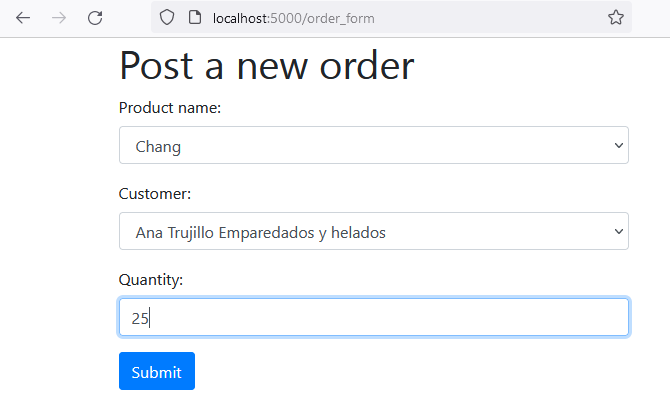
\includegraphics[width=0.75\linewidth,height=\textheight,keepaspectratio]{./images/img-072-066.png}

\begin{itemize}
\tightlist
\item
  A felhasználó egy legördülő listából kiválaszthat egy terméket,
  megadhat egy mennyiséget, és feladhat egy rendelést a Northwind
  adatbázisban. A visszaadott oldal megerősíti a rendelést, és listázza
  az utolsó 5 rendelést.
\item
  Az alkalmazás hibaüzenetet ad, ha a termék készlete vagy az ügyfél
  egyenlege túl alacsony.
\item
  A rendelés feladása tranzakcióban fut.
\end{itemize}

\subsubsection{A demóalkalmazás futtatása localhostról Postgres
háttérrel}\label{a-demuxf3alkalmazuxe1s-futtatuxe1sa-localhostruxf3l-postgres-huxe1ttuxe9rrel}

Végezd el a következő lépéseket:

\begin{enumerate}
\def\labelenumi{\arabic{enumi}.}
\item
  (\emph{már telepítve a VM-en}) Telepítsd az Anaconda Pythont.
\item
  (\emph{már telepítve a VM-en}) Hozz létre virtuális környezetet a
  projekthez:\footnote{Lásd:
    https://blog.usejournal.com/why-and-how-to-make-a-requirements-txt-f329c685181e}

  \begin{itemize}
  \tightlist
  \item
    Anaconda admin prompt:
    \texttt{set\ https\_proxy=http://proxy.uni-pannon.hu:3128}
  \item
    \texttt{http://proxy.mik.uni-pannon.hu}
  \item
    (ellenkező esetben `SSL: WRONG\_VERSION\_NUMBER' hibát kapsz)
  \item
    \texttt{conda\ create\ -n\ flask\_demo\ pip} //python=3.8.5
  \item
    python verzió: \texttt{python\ -version} //3.9.11
  \item
    elérhető virtuális környezetek: \texttt{conda\ env\ list}
  \item
    \texttt{conda\ activate\ flask\_demo} (később telepítjük a szükséges
    csomagokat)
  \item
    \texttt{pip\ install\ flask}
  \item
    \texttt{pip\ install\ psycopg2}
  \end{itemize}
\item
  Töltsd le a \texttt{northwind.py} alkalmazást, és lépj be a Flask
  projekt mappájába (vagyis a \texttt{flask} nevű könyvtárba).
\item
  Indítsd el az Anaconda Spyder Python szerkesztőt, és állítsd be a
  jelszót és az 5432-es portot a 59. sorban. Nézd át az alkalmazást.
  Megjegyzendő, hogy a \texttt{with\ connection:} blokk a
  \texttt{new\_order()} függvény hívását \textbf{tranzakcióban}
  futtatja.
\item
  A conda parancssorban: \texttt{set\ FLASK\_APP=northwind.py} (a
  \texttt{DEBUG=1} beállítással nem kell manuálisan újraindítani a
  webszervert minden módosítás után). Megjegyzés: a GCP-n
  \texttt{main.py} névként fogjuk használni, így ott nincs szükség
  különleges beállításra.
\item
  \texttt{flask\ run}
\item
  Teszteld a lapot a \texttt{http://localhost:5000/order\_form} címen.
  Felhasznált technológiák:

  \begin{itemize}
  \tightlist
  \item
    \begin{enumerate}
    \def\labelenumii{\alph{enumii}.}
    \tightlist
    \item
      A \texttt{templates} mappa tartalmazza a jinja template engine
      által feldolgozott HTML lapokat. A Python változók elérhetők a
      HTML sablonokban
      (\texttt{\{\%\ for\ ...\ in\ /\ if\ ...else\ /\ with\ /\ block,\ extends\ \%\}}),
      és a sablonok egymásba ágyazhatók a `block'
      segítségével.\footnote{Flask app:
        https://www.youtube.com/watch?v=MwZwr5Tvyxo / HTML sablonok:
        https://www.youtube.com/watch?v=QnDWlZuWYW0}
    \end{enumerate}
  \item
    \begin{enumerate}
    \def\labelenumii{\alph{enumii}.}
    \setcounter{enumii}{1}
    \tightlist
    \item
      Bootstrap (formázáshoz)
    \end{enumerate}
  \end{itemize}
\item
  Az alkalmazás tovább javítható vagy biztonságosabbá tehető, de ez most
  nem célunk.\footnote{WTF Forms:
    https://www.youtube.com/watch?v=UIJKdCIEXUQ / Database ORM:
    https://www.youtube.com/watch?v=cYWiDiIlUxQc}
\end{enumerate}

\begin{center}\rule{0.5\linewidth}{0.5pt}\end{center}

\subsection{Dokumentumtárolók: A Cloud Firestore
áttekintése}\label{dokumentumtuxe1roluxf3k-a-cloud-firestore-uxe1ttekintuxe9se}

Ezt az alkalmazást a Google Cloud Firestore-ba migráljuk. A Google Cloud
Firestore egy dokumentumtároló. Több dokumentumgyűjtemény tárolását
támogatja. A korábbi Realtime Database új kiadása, amely egyetlen
monolitikus JSON-t használt.\footnote{Összehasonlításért lásd:
  https://firebase.google.com/docs/firestore/rtdb-vs-firestore\#key\_considerations}
A Cloud Firestore jellemzői:

\begin{itemize}
\item
  „Firestore adatbázis = dokumentumok gyűjteményei''.
\item
  Minden dokumentum lényegében egy JSON dokumentum, pl.:

\begin{verbatim}
name :
      first : "Joe"
      last : "Long"
born : 1995
\end{verbatim}
\item
  A gyűjtemény \textbf{nem kényszerít ki sémát}, vagyis tetszőleges
  szerkezetű dokumentumokat tárolhat ugyanabban a gyűjteményben.
  Mindazonáltal még ha nincs is sémaellenőrzés beszúráskor, minden
  valósághű alkalmazás, amely a gyűjteményt olvassa, egy bizonyos sémát
  vár --- ez a \textbf{schema-on-read (olvasáskori séma)} rendszer. Ez
  ellentétben áll a relációs adatbázisok \textbf{schema-on-write
  (íráskori séma)} megközelítésével, ahol a sémának nem megfelelő írások
  nem engedélyeztek.
\item
  Minden dokumentumnak egyedi kulcsa kell legyen, amely automatikusan
  generálható, de \textbf{nem lehet kizárólag szám}.
\item
  A gyűjtemények nem ágyazhatók egymásba. Egy dokumentum azonban
  tartalmazhat egy hozzá csatolt algyűjteményt, egy
  coll-doc-coll-doc-coll-\ldots{} stb. hierarchiában, legfeljebb 100
  mélységig.
\item
  Speciális dokumentum adattípusok: 1-D tömb, map (asszociatív tömb),
  reference típus. A referencia egy dokumentumhoz vezető elérési út
  string, pl. egy hierarchiában lévő dokumentumra mutató referencia.
  Formája lehet: \texttt{coll\_id/doc\_id/coll\_id/...} stb.
  Algyűjteményekkel kapcsolatos lehetséges probléma, hogy `árva'
  állapotban is fennmaradhatnak, ha a szülő gyűjtemény törlésre kerül.
\item
  Az egy-a-többhöz kapcsolatok beágyazással valósíthatók meg; \textbf{a
  több-a-többhöz gyűjtemények beágyazás és referenciák kombinációjával}
  valósíthatók meg.
\item
  A Firestore valós idejű egyidejű frissítéseket és atomi tranzakciókat
  támogat. A lekérdezések szűrőkkel valósíthatók meg.
\item
  Egy Realtime/snapshot listener eseményt generál, amikor egy dokumentum
  megváltozik, és egy alkalmazás egy visszahívó függvénnyel (callback)
  feliratkozhat erre az eseményre.\footnote{Lásd:
    https://firebase.google.com/docs/firestore/query-data/listen}
\end{itemize}

\subsubsection{A Firestore dokumentumtárunk tervezése, létrehozása és
feltöltése}\label{a-firestore-dokumentumtuxe1runk-tervezuxe9se-luxe9trehozuxe1sa-uxe9s-feltuxf6ltuxe9se}

Az adatokat újra kell modellezni --- ez alkalmazásfüggő folyamat.
Tervezett lekérdezéseink:

\begin{itemize}
\tightlist
\item
  Termékek és ügyfelek listázása
\item
  Új rendelés feladása egyetlen tétellel
\item
  Az utolsó 5 rendelési tétel listázása a rendelés- és ügyfélAdatokkal
\end{itemize}

E lekérdezések figyelembevételével 3 gyűjteményt tervezünk: egy lapos
Products, egy lapos Customer és egy hierarchikus Orders→Orderitems
gyűjteményt. Megjegyzendő, hogy ez nem illik jól egy olyan
lekérdezéshez, amely azt kérdezi, mi lett megrendelve és mikor --- de
ilyen lekérdezés (még) nem része az alkalmazásunknak.

Alternatívaként az Orders→Orderitems gyűjteményt a Customers
gyűjteménybe ágyazhatnánk, de ez megnehezítené az időrend szerinti
rendeléslista lekérdezését, mivel az algyűjtemények lekérdezése
általában \textbf{nem engedélyezett} a szülő dokumentumgyűjtemény
iterálása nélkül.

Egyéb megfontolások:

\begin{itemize}
\tightlist
\item
  Automatikus dokumentum ID-kat használunk
\item
  A rendeléseket dátum szerint rendezzük az utolsó 5 tétel listázásának
  támogatásához
\item
  A CustomerID automatikusan indexelődik
\end{itemize}

A migrációs folyamatnak 2 fő lépése van:

\begin{enumerate}
\def\labelenumi{\arabic{enumi}.}
\tightlist
\item
  Az új adatbázis megvalósítása és az adatok átalakítása/betöltése
\item
  A kliens alkalmazás újraimplementálása az új adatbázishoz
\end{enumerate}

\textbf{Az új adatbázis megvalósítása és az adatok
átalakítása/betöltése}

A dokumentumtárat programozottan hozzuk létre és töltjük fel: a
localhostlon futó Postgres adatbázisból olvasunk, és a felhőbeli
dokumentumtárba írunk.

GCP szolgáltatásfiókot kell létrehozni a Firebase tároló eléréséhez az
asztali gépünkről.\footnote{Az alkalmazáson belüli GCP-projektből nem
  lenne szükségünk szolgáltatásfiókra a tároló eléréséhez, de sokkal
  egyszerűbb és gyorsabb az alkalmazást helyben fejleszteni és
  hibakeresni, majd szükség esetén GCP-re telepíteni. Lásd még:
  https://cloud.google.com/compute/docs/access/create-enable-service-accounts-for-instances}

\begin{enumerate}
\def\labelenumi{\arabic{enumi}.}
\item
  Nyisd meg a Firebase konzolt: https://console.firebase.google.com/

  \begin{itemize}
  \tightlist
  \item
    \begin{enumerate}
    \def\labelenumii{\alph{enumii}.}
    \tightlist
    \item
      Google-hitelesítés után hozz létre egy új projektet
    \end{enumerate}
  \item
    \begin{enumerate}
    \def\labelenumii{\alph{enumii}.}
    \setcounter{enumii}{1}
    \tightlist
    \item
      Nincs szükség sem Gemini-re, sem Google Analytics-re ebben a
      projektben
    \end{enumerate}
  \item
    \begin{enumerate}
    \def\labelenumii{\alph{enumii}.}
    \setcounter{enumii}{2}
    \tightlist
    \item
      Lépj a
      https://console.firebase.google.com/u/0/project/{[}Your\_project\_ID{]}/firestore
      oldalra, és hozz létre egy adatbázist. Kísérletezz manuálisan
      gyűjtemények és dokumentumok
      hozzáadásával/törlésével/szerkesztésével itt vagy a GCP felületen.
    \end{enumerate}
  \item
    \begin{enumerate}
    \def\labelenumii{\alph{enumii}.}
    \setcounter{enumii}{3}
    \tightlist
    \item
      Hozz létre egy \texttt{books} nevű gyűjteményt két
      könyv-dokumentummal
    \end{enumerate}
  \item
    \begin{enumerate}
    \def\labelenumii{\alph{enumii}.}
    \setcounter{enumii}{4}
    \tightlist
    \item
      A Firebase konzolban: fogaskerék ikon → Service accounts → Create
      service account → Generate new private key. Itt generálhatunk egy
      JSON-fájlt, amely az automatikusan létrehozott szolgáltatásfiók
      kulcsát tartalmazza. Mentsd el ezt a fájlt biztonságos helyre,
      mert hozzáférést biztosít az adatbázishoz.
    \end{enumerate}
  \item
    \begin{enumerate}
    \def\labelenumii{\alph{enumii}.}
    \setcounter{enumii}{5}
    \tightlist
    \item
      Python kód is találhető itt a csatlakozáshoz.
    \end{enumerate}
  \end{itemize}
\item
  (\emph{már telepítve a VM-en}) A conda parancssorban, lépj a virtuális
  környezetbe és futtasd: \texttt{pip\ install\ firebase\_admin}
\item
  Mostantól csatlakozni tudsz az adatbázishoz:
  \texttt{db\ =\ firestore.client()}

  \begin{itemize}
  \tightlist
  \item
    \begin{enumerate}
    \def\labelenumii{\alph{enumii}.}
    \tightlist
    \item
      Ellenőrizd, hogy a Postgres szolgáltatás fut, és a Northwind
      táblák elérhetők
    \end{enumerate}
  \item
    \begin{enumerate}
    \def\labelenumii{\alph{enumii}.}
    \setcounter{enumii}{1}
    \tightlist
    \item
      Győződj meg arról, hogy a proxy KI van kapcsolva a VM-en
    \end{enumerate}
  \item
    \begin{enumerate}
    \def\labelenumii{\alph{enumii}.}
    \setcounter{enumii}{2}
    \tightlist
    \item
      Tekintsd át és futtasd a \texttt{flask\_gcp\_firestore} mappában
      lévő \texttt{main.py} Python szkriptet, amely betölti a 3
      gyűjteményt. Ehhez nincs szükség Flask webszerverre; a szkriptet a
      conda parancssorból is elindíthatod:
      \texttt{python\ main.py}\footnote{Ha hitelesítési hibát kapsz, az
        valószínűleg a virtuális gép helytelen rendszeridő-beállítása
        miatt van. A dátum és idő beállítás rendszerpanelén módosítsd a
        rendszeridőt kézire, majd vissza automatikusra az idő
        frissítéséhez.}
    \end{enumerate}
  \item
    \begin{enumerate}
    \def\labelenumii{\alph{enumii}.}
    \setcounter{enumii}{3}
    \tightlist
    \item
      Ellenőrizd a gyűjtemények tartalmát a Firebase konzolban.
    \end{enumerate}
  \end{itemize}
\end{enumerate}

\begin{quote}
\textbf{GYAKORLAT:} tekintsd át és futtasd az új \texttt{northwind.py}
webalkalmazást, amely a Firestore adatbázist használó
rendelés-feldolgozási tranzakciót valósítja meg.

\begin{itemize}
\tightlist
\item
  Manuálisan töröld a \texttt{main.py} által beszúrt demo rendelést.
\item
  Valósítsd meg a hiányzó \texttt{list\_orders()} függvényt, amely
  összegző sort ad vissza az utolsó 5 rendelés minden rendelési
  tételéhez. Az eredményt az \texttt{order\_list.html} sablon jeleníti
  meg.
\end{itemize}

A reprodukálandó funkcionalitás a következő:

\begin{Shaded}
\begin{Highlighting}[]
\KeywordTok{select}\NormalTok{ o.orderdate:}\CharTok{:timestamp}\NormalTok{(}\DecValTok{0}\NormalTok{) }\KeywordTok{without} \DataTypeTok{time} \DataTypeTok{zone} \KeywordTok{as}\NormalTok{ orderdate,}
\NormalTok{c.companyname, c.country, c.balance, p.productname, od.quantity,}
\NormalTok{od.quantity }\OperatorTok{*}\NormalTok{ od.unitprice }\KeywordTok{as} \FunctionTok{value}\NormalTok{, p.unitsinstock}
\KeywordTok{from}\NormalTok{ products p }\KeywordTok{join}\NormalTok{ orderdetails od }\KeywordTok{on}\NormalTok{ p.productid}\OperatorTok{=}\NormalTok{od.productid}
    \KeywordTok{join}\NormalTok{ orders o }\KeywordTok{on}\NormalTok{ o.orderid}\OperatorTok{=}\NormalTok{od.orderid}
    \KeywordTok{join}\NormalTok{ customers c }\KeywordTok{on}\NormalTok{ c.customerid}\OperatorTok{=}\NormalTok{o.customerid}
\KeywordTok{order} \KeywordTok{by}\NormalTok{ orderdate }\KeywordTok{desc} \KeywordTok{limit} \DecValTok{5}\NormalTok{;}
\end{Highlighting}
\end{Shaded}

\begin{itemize}
\tightlist
\item
  Ugyanazokat a HTML sablonokat használhatod.
\item
  Teszteld a webalkalmazást a \texttt{http://localhost:5000/} címen.
\end{itemize}
\end{quote}

\begin{center}\rule{0.5\linewidth}{0.5pt}\end{center}

\subsection{Az adatintegritás érvényesítésének
összehasonlítása}\label{az-adatintegrituxe1s-uxe9rvuxe9nyesuxedtuxe9suxe9nek-uxf6sszehasonluxedtuxe1sa}

Az alábbi táblázat összehasonlítja a Postgres és Firestore
adatintegritást érvényesítő eszközeit:

\begin{longtable}[]{@{}
  >{\raggedright\arraybackslash}p{(\linewidth - 2\tabcolsep) * \real{0.2990}}
  >{\raggedright\arraybackslash}p{(\linewidth - 2\tabcolsep) * \real{0.7010}}@{}}
\toprule\noalign{}
\begin{minipage}[b]{\linewidth}\raggedright
\textbf{Postgres}
\end{minipage} & \begin{minipage}[b]{\linewidth}\raggedright
\textbf{Firestore}
\end{minipage} \\
\midrule\noalign{}
\endhead
\bottomrule\noalign{}
\endlastfoot
A séma minden DML-műveletben érvényesített: `schema on write' & Egy
gyűjtemény minden dokumentumának eltérő attribútumai (mezői) lehetnek:
`schema on read' \\
Gazdag adattípus-készlet és felhasználó által definiált adattípusok (pl.
enumerációs típusok) & Nagyon korlátozott adattípus-készlet, pl. nincs
pénz vagy decimális típus \\
Elsődleges kulcsok és idegen kulcsok & A gyűjtemény azonosítójának
egyedinek kell lennie és automatikusan generálható (mint a serial
típus), de nem lehet kizárólag szám. Az idegen kulcsok attribútumként
tárolhatók és biztonsági szabályokkal érvényesíthetők. \\
Egyedi megszorítások és check-megszorítások & Biztonsági
szabályok\footnote{A Firebase Admin SDK-t használó kliensalkalmazás
  adminisztrátori jogosultságokkal fut, és megkerüli a Firestore
  adatbázishoz definiált biztonsági szabályokat. Biztonsági szabályokat
  csak mobil kliensen lehet bemutatni. Ezért a szabályok ebben a
  szövegben nem kerülnek részletezésre. Bővebb információért lásd:
  https://firebase.google.com/docs/firestore/security/get-started} \\
ACID tranzakciós biztonság támogatott & A tranzakciók elindíthatók a
kliensről a test-and-set típusú hibák megelőzésére, és az atomicitás
kötegelt írásokkal megőrizhető,\footnote{Lásd:
  https://firebase.google.com/docs/firestore/manage-data/transactions\#python\_1}
de a tranzakciók nem kombinálhatók kötegelt írásokkal (lásd később). \\
\end{longtable}

\begin{center}\rule{0.5\linewidth}{0.5pt}\end{center}

\subsection{Tranzakciók Firestore-ban és
Postgres-ben}\label{tranzakciuxf3k-firestore-ban-uxe9s-postgres-ben}

\begin{quote}
\textbf{DEMO:} teszteld a rendelési tranzakció atomicitását
Postgres-ben. A PgAdmin konzolban injektálj hibát a
\texttt{new\_order()} függvénybe az alábbi utasítás felülírásával:

\begin{Shaded}
\begin{Highlighting}[]
\KeywordTok{insert} \KeywordTok{into}\NormalTok{ orders (orderid, customerid) }\KeywordTok{values}\NormalTok{ (var\_orderid, var\_custid);}
\end{Highlighting}
\end{Shaded}

ezzel az utasítással:

\begin{Shaded}
\begin{Highlighting}[]
\KeywordTok{insert} \KeywordTok{into}\NormalTok{ orders (orderid, customerid) }\KeywordTok{values}\NormalTok{ (var\_orderid, }\StringTok{\textquotesingle{}ERROR\textquotesingle{}}\NormalTok{);}
\end{Highlighting}
\end{Shaded}

Ez idegen kulcs-megszorítást sért, és futásidejű hibát okoz a következő
hívásnál. A webalkalmazást használva adj fel egy új rendelést, és
ellenőrizd, hogy a hiba után az ügyfél egyenlege visszaáll az eredeti
értékre --- annak ellenére, hogy az INSERT utasítás előtt már csökkentve
lett. \emph{A tranzakció automatikusan visszagörgetett.}
\end{quote}

\begin{quote}
\textbf{DEMO:} logikai hibák Firestore-ban párhuzamos környezetben

\begin{itemize}
\tightlist
\item
  Adj hozzá 10 másodperces késleltetést a készlet és egyenleg
  ellenőrzése után (\texttt{import\ time} és \texttt{time.sleep(10)})
\item
  Állítsd be kézzel mindhárom ügyfél egyenlegét 10 000-re, és a Chai
  termék készletét 3-ra a Cloud Firestore webkonzolon
\item
  Indítsd el az alkalmazást 3 böngészőablakban, és rendelj mindegyik
  ügyfélnek 2 egység Chai-t (értéke: 2×18=36). Elvárjuk, hogy a
  korlátozott készlet miatt \emph{csak egy rendelés legyen sikeres}.
\item
  Ellenőrizd: mindhárom rendelés SUCCESS eredménnyel kerül
  feldolgozásra, mindhárom ügyfél egyenlege 36-tal csökken, és az új
  készlet 1. Látható, hogy tranzakciós ellenőrzés nélkül \emph{súlyos
  logikai hibák fordulhatnak elő}.
\end{itemize}
\end{quote}

\subsubsection{Firestore-tranzakció
használata}\label{firestore-tranzakciuxf3-hasznuxe1lata}

Egy Firestore-tranzakció olvasási műveleteket tartalmazhat, amelyeket
írási műveletek követnek. \emph{Ha egy tranzakció olvas egy
dokumentumot, majd a dokumentumot egy másik kliens módosítja a commit
előtt, a tranzakció automatikusan visszagörgetésre kerül és
újrafuttatódik (legfeljebb 5-ször).} Az atomicitás egyetlen commit
művelet szintjén garantált, de párhuzamos módosítások esetén a
tranzakció újrafuttatása szükséges lehet. Példa:

\begin{Shaded}
\begin{Highlighting}[]
\CommentTok{\# create a new customer called test manually and set its balance to 9}
\CommentTok{\# then run this script in two parallel sessions}

\ImportTok{import}\NormalTok{ firebase\_admin}
\ImportTok{from}\NormalTok{ firebase\_admin }\ImportTok{import}\NormalTok{ credentials}
\ImportTok{from}\NormalTok{ firebase\_admin }\ImportTok{import}\NormalTok{ firestore}
\ImportTok{import}\NormalTok{ time}

\NormalTok{cred }\OperatorTok{=}\NormalTok{ credentials.Certificate(}\StringTok{"token.json"}\NormalTok{)}
\NormalTok{firebase\_admin.initialize\_app(cred)}
\NormalTok{db }\OperatorTok{=}\NormalTok{ firestore.client()}
\NormalTok{transaction }\OperatorTok{=}\NormalTok{ db.transaction()}
\NormalTok{cust\_ref }\OperatorTok{=}\NormalTok{ db.collection(}\StringTok{\textquotesingle{}customers\textquotesingle{}}\NormalTok{).document(}\StringTok{\textquotesingle{}test\textquotesingle{}}\NormalTok{)}

\AttributeTok{@firestore.transactional}
\KeywordTok{def}\NormalTok{ update\_in\_transaction(transaction, cust\_ref):}
\NormalTok{  cust\_ref\_snapshot }\OperatorTok{=}\NormalTok{ cust\_ref.get(transaction}\OperatorTok{=}\NormalTok{transaction)}
\NormalTok{  new\_balance }\OperatorTok{=}\NormalTok{ cust\_ref\_snapshot.get(}\StringTok{\textquotesingle{}balance\textquotesingle{}}\NormalTok{) }\OperatorTok{+} \DecValTok{1}
  \BuiltInTok{print}\NormalTok{(}\StringTok{"New balance: "}\NormalTok{, new\_balance)}
\NormalTok{  time.sleep(}\DecValTok{10}\NormalTok{)}
  \ControlFlowTok{if}\NormalTok{ (new\_balance }\OperatorTok{\textless{}=} \DecValTok{10}\NormalTok{):}
\NormalTok{    transaction.update(cust\_ref, \{}\StringTok{\textquotesingle{}balance\textquotesingle{}}\NormalTok{: new\_balance\})}
    \BuiltInTok{print}\NormalTok{(}\StringTok{"Balance increased"}\NormalTok{)}
  \ControlFlowTok{else}\NormalTok{:}
    \BuiltInTok{print}\NormalTok{(}\StringTok{"Balance already maximal"}\NormalTok{)}

\NormalTok{update\_in\_transaction(transaction, cust\_ref)}
\end{Highlighting}
\end{Shaded}

Állítsd be a tesztvevő egyenlegét kézzel 9-re, majd futtasd a fenti
szkriptet két párhuzamos munkamenetből. Bár mindkét munkamenetből
megkapjuk a `Balance increased' üzenetet, a végső egyenleg 10 lesz (és
nem 11), mivel az egyik tranzakció (amelyik a `Balance already maximal'
üzenetet adta vissza) visszagörgetésre került és újrafuttatódott. Ezért
\emph{sikerült érvényesítenünk azt az üzleti szabályt, hogy az egyenleg
nem haladhatja meg a 10-et}, még párhuzamos esetben sem.

\begin{quote}
\textbf{GYAKORLAT:} a fenti kódrészletet sablonként használva add hozzá
a tranzakciós vezérlést a Firestore-alapú Python Flask alkalmazás
\texttt{order\_proc} függvényéhez, és teszteld a helyes működését a
Párhuzamossági demó részben leírt forgatókönyvben. Elvárjuk, hogy több
párhuzamos tranzakció közül \emph{csak egy} fusson sikeresen, és az
adatbázis konzisztenciája megmaradjon. Ez azt jelenti, hogy az összes
tranzakció végén a készlet helyes legyen, \emph{csak egy} rendelés
kerüljön elfogadásra, és \emph{csak egy} ügyfél egyenlege csökkenjen.
\end{quote}

\subsubsection{Kötegelt írások (Batched
writes)}\label{kuxf6tegelt-uxedruxe1sok-batched-writes}

Több `doc.set', `update' vagy `delete' műveletet tartalmazó köteg
atomicitása a \texttt{db.batch()} objektummal érvényesíthető.
Megjegyzendő, hogy ez a megoldás nem nyújt védelmet a kliens által már
beolvasott dokumentumokon végrehajtott külső frissítések ellen --- ezért
\emph{nem képes megakadályozni a `test-and-set' típusú logikai
hibákat.}\footnote{Vö.: „Firestore allows you to run sophisticated ACID
  transactions against your document data.''
  https://cloud.google.com/firestore}

\emph{Nem lehetséges kötegelt írásokat tranzakcióba ágyazni. Ezért
dönteni kell: az ACID-követelmények atomicitása vagy az izoláció
biztosítása a cél.}

A tranzakciók csak online működnek, azaz szerverkapcsolat szükséges, de
a kötegelt írások offline is működhetnek.

\begin{quote}
\textbf{DEMO:} tekintsd át és teszteld a demóalkalmazás kötegelt verziót
(\texttt{northwind\_batch\_write.py}) egy futásidejű hiba
injektálásával, pl. \texttt{print(1/0)} két írás közé.
\end{quote}

Néhány további Firestore-korlát:

\begin{itemize}
\tightlist
\item
  Egy tranzakció vagy köteg legfeljebb 500 dokumentumba írhat
\item
  Az olvasási műveleteket (\texttt{get()}) a írási műveletek
  (\texttt{set()}, \texttt{update()}) előtt kell elvégezni
\item
  „A tranzakciókra vagy kötegelt írásokra vonatkozó biztonsági
  szabályokban az atomi művelet egészére vonatkozóan legfeljebb 20
  dokumentum-hozzáférési hívás engedélyezett, a kötegben lévő minden
  egyes dokumentumra vonatkozó normál 10 hívási korláton felül.''
\item
  stb. \ldots{}
\end{itemize}

\emph{Általános következtetésként megállapítható, hogy a
NoSQL-technológiák esetén a kliensnek (vagy az üzleti logikai rétegnek)
kell támogatnia és megvalósítania az összes alacsony szintű
adatfeldolgozási műveletet, mint például gyűjtemények összekapcsolása
stb. A tranzakciós vezérlés és az adatintegritás érvényesítése is
kevésbé robusztus a relációs adatbázis-technológiákhoz képest. Ezért a
NoSQL-technológiák viszonylag \textbf{egyszerű üzleti területek és
folyamatok} esetén ajánlhatók --- például egy bloggeroldal esetén.}

\subsubsection{Egyéb érdekes Firestore-funkciók (nem
részletezve)}\label{egyuxe9b-uxe9rdekes-firestore-funkciuxf3k-nem-ruxe9szletezve}

\begin{itemize}
\tightlist
\item
  Valós idejű frissítések
\item
  Offline adatpersistálás
\item
  Integráció felhőszolgáltatásokkal
\end{itemize}

\begin{center}\rule{0.5\linewidth}{0.5pt}\end{center}

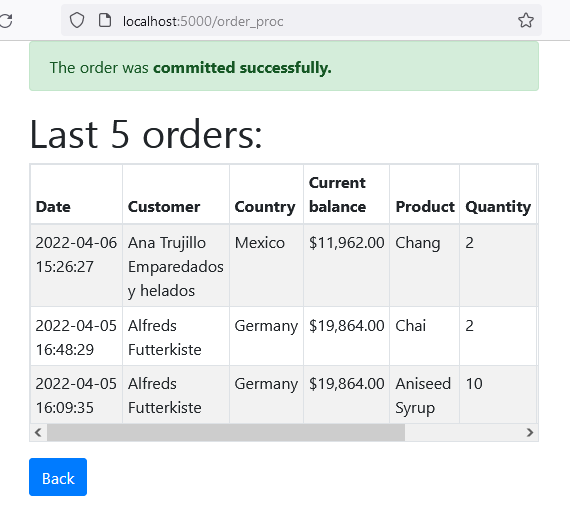
\includegraphics[width=0.75\linewidth,height=\textheight,keepaspectratio]{./images/img-073-067.png}

\section{7. Felhőalapú
adatbázis-technológiák}\label{felhux151alapuxfa-adatbuxe1zis-technoluxf3giuxe1k}

\subsection{Áttekintés}\label{uxe1ttekintuxe9s}

Az olyan felhőszolgáltatók, mint az Amazon, a Google, az IBM és a
Microsoft, adatbázis-kezelési szolgáltatásokat kínálnak SaaS vagy PaaS
alapon. Egy ilyen megoldás alkalmazhatósága a saját adatbázis-szerverek
futtatásával szemben gazdasági és részben műszaki szempontoktól függ.
Néhány szempont:

\textbf{Előnyök:}

\begin{itemize}
\tightlist
\item
  A felhőszolgáltatások magas rendelkezésre állást (a vállalati
  szervereket meghaladó szinten) nyújtanak, földrajzilag elosztott
  infrastruktúrával.
\item
  A felhőszolgáltatások automatizált, igény szerinti méretezhetőséget
  kínálnak rugalmas, legalább részben terhelésfüggő számlázási sémákkal.
\item
  A felhő számos egyéb felhőn belüli szolgáltatást is kínál, mint
  például adatelemzés, képfeldolgozás, NLP stb., amelyek hozzáférnek a
  felhőalapú adatbázishoz, és integrálhatók egy megoldásba.
\end{itemize}

\textbf{Hátrányok:}

\begin{itemize}
\tightlist
\item
  A felhőalapú adatbázis-szolgáltatások által nyújtott funkcionalitás
  jellemzően korlátozottabb, mint a saját szervereké, bár egyes funkciók
  más eszközökkel pótolhatók.
\item
  Bár egyes költségek arányosak a felhasználással, fix költségek is
  vannak, pl. az adattárolásé. Ezeket a tervezett szolgáltatás vagy
  megoldás üzleti tervében figyelembe kell venni.
\item
  Az adatbiztonság veszélybe kerülhet, ha erősen érzékeny adatok (pl.
  személyes egészségügyi rekordok) fizikailag elhagyják a vállalati
  hálózatot. Biztonsági incidensek vagy súlyos adatvesztés is
  előfordulhat.\footnote{Lásd:
    https://www.theguardian.com/australia-news/article/2024/may/09/unisuper-google-cloud-issue-account-access}
\item
  A kritikus szolgáltatások, pl. a gyártásvezérlő rendszerek nem
  függhetnek az internet-hozzáféréstől. Ez utóbbi két aggályt egy
  \textbf{privát felhő}\footnote{Pl. https://www.openstack.org/}
  enyhítheti.
\end{itemize}

\begin{center}\rule{0.5\linewidth}{0.5pt}\end{center}

\subsection{Új GCP-projekt
indítása}\label{uxfaj-gcp-projekt-induxedtuxe1sa}

Ebben a projektben az App Engine-t használjuk a Flask alkalmazás
futtatásához, egy felhőalapú SQL adatbázist és egy Firestore
dokumentumtárat.

\begin{enumerate}
\def\labelenumi{\arabic{enumi}.}
\tightlist
\item
  Indíts el egy privát böngészőt, és engedélyezd a felugró ablakokat.
\item
  Aktiváld a 50 dolláros kupont az egyetemi e-mail-címeddel, az
  Neptun-üzenetben kapott utasítások szerint.
\item
  Lépj be a https://console.cloud.google.com oldalra.
\item
  Indíts el egy új projektet, vagy töröld a meglévőt: IAM \& Admin →
  Manage resources.
\item
  Meg kell adnod egy globálisan egyedi projektnevet, amelyre ebben a
  kézikönyvben YOUR-PROJECT-ID-ként hivatkozunk. Ellenőrizd a projekthez
  kapcsolt számlát --- induláskor 50 dolláros kredittel kell
  rendelkeznie.
\item
  A Firestore oldalon válaszd: SELECT NATIVE MODE, majd CREATE DATABASE.
  Egy GCP-projektben csak egyetlen Firestore adatbázis engedélyezett.
\end{enumerate}

\begin{center}\rule{0.5\linewidth}{0.5pt}\end{center}

\subsection{A Postgres adatbázis migrálása
GCP-re}\label{a-postgres-adatbuxe1zis-migruxe1luxe1sa-gcp-re}

\begin{enumerate}
\def\labelenumi{\arabic{enumi}.}
\tightlist
\item
  GCP Databases → SQL → Create instance → PostgreSQL (engedélyezni kell
  a Compute Engine API-t).
\item
  Válassz egy példányazonosítót és jelszót. A példány neve az
  adatbázis-szerver neve, nem az adatbázisé vagy az
  adatbázis-felhasználóé. Állítsd be:

  \begin{itemize}
  \tightlist
  \item
    Régió: Europe, PostgreSQL 13-as verzió, single zone (feladatátvétel
    nélkül)
  \item
    Testreszabás: publikus IP engedélyezve
  \end{itemize}
\item
  Kapcsolatok: „Ebben a projektben az összes alkalmazás
  alapértelmezetten engedélyezett'', azonban tervezzük az adatbázis
  elérését az interneten keresztül PgAdmin-ból, ezért engedélyezünk
  bármilyen IP-t (=pg\_hba.conf bejegyzés). Hálózat hozzáadása:
  \texttt{0.0.0.0/0}. Mentés.
\item
  A Speciális beállításokban (Advanced options) engedélyezd a Query
  Insights funkciót.
\item
  Várd meg, amíg a példány elkészül, majd változtasd meg a
  Postgres-felhasználó jelszavát. Az SQL Overview-ra navigálva
  megtalálod a szerver publikus IP-címét.
\item
  PgAdmin-ban csatlakozz a felhőpéldányhoz a publikus IP-cím
  segítségével, majd tekintsd át és futtasd a \texttt{pg\_script.sql}
  dump-fájlt.
\item
  Módosítsd a Python alkalmazásban az IP-t a nyilvános GCP IP-re, és
  teszteld az alkalmazást. Az új rendeléseknek meg kell jelenniük a
  Postgres táblákban.
\item
  Visszatérve a GCP-re, nyisd meg a Query Insights-ot, és ellenőrizd a
  \texttt{SELECT\ *\ FROM\ last\_orders} lekérdezés végrehajtási tervét.
  Megjegyzendő, hogy egy lekérdezés megjelenése a Query Insights
  statisztikákban akár 10 percet is igénybe vehet --- ez egy offline
  elemzési eszköz.
\end{enumerate}

\begin{center}\rule{0.5\linewidth}{0.5pt}\end{center}

\subsection[A demóalkalmazás megvalósítása GCP-n → Cloud programozás MSc
kurzus]{\texorpdfstring{A demóalkalmazás megvalósítása GCP-n\footnote{Ha
  már jól ismered a felhőprogramozási koncepciókat, kihagyhatod ezt a
  részt, és folytathatod az alkalmazással localhostról futtatva.} →
Cloud programozás MSc
kurzus}{A demóalkalmazás megvalósítása GCP-n → Cloud programozás MSc kurzus}}\label{a-demuxf3alkalmazuxe1s-megvaluxf3suxedtuxe1sa-gcp-n33-cloud-programozuxe1s-msc-kurzus}

Az alkalmazást a GCP App Engine-re telepítjük.\footnote{Lásd:
  https://medium.com/@dmahugh\_70618/deploying-a-flask-app-to-google-app-engine-faa883b5ffab}

\begin{enumerate}
\def\labelenumi{\arabic{enumi}.}
\item
  (\emph{már telepítve a VM-en}) Telepítsd a Cloud SDK-t és a gcloud
  CLI-t az asztali számítógépedre.
\item
  Nyiss meg egy cmd terminált \textbf{Windows rendszergazdaként}, lépj
  be a \texttt{flask\_gcp} könyvtárba, és állítsd be:
  \texttt{HTTPS\_PROXY=http://proxy.uni-pannon.hu:3128}
\item
  A parancssorban: \texttt{gcloud\ init} (saját Google-profillal való
  hitelesítés szükséges), majd válaszd ki a YOUR-PROJECT-ID-t.
\item
  Az SDK nem tartalmazza az App Engine bővítményt, ezért ezt külön kell
  telepíteni. A Google Cloud SDK shell parancssorában:
  \texttt{gcloud\ components\ install\ app-engine-python}. Ez néhány
  percet vesz igénybe.
\item
  \texttt{gcloud\ config\ set\ project\ YOUR-PROJECT-ID}
\item
  \texttt{//check\ billing:}
  \texttt{gcloud\ beta\ billing\ accounts\ list}
\item
  A \texttt{northwind.py} szkriptben módosítsd az adatbázis-kapcsolati
  paramétereket a nyilvános GCP IP-re, és mentsd el \texttt{main.py}
  névvel. (Frissítsd a \texttt{requirements.txt} fájlt is.)
\item
  A tároló (container) futtatásához a Cloud Build API szükséges, ezért
  ezt engedélyezni kell a projektben:
  \texttt{gcloud\ services\ enable\ cloudbuild.googleapis.com}
\item
  Inicializáld az App Engine-t a projektben:
  \texttt{gcloud\ app\ create\ -\/-project=YOUR-PROJECT-ID}
\item
  \texttt{gcloud\ app\ deploy} Megkapod a cél URL-t, amelyen az
  alkalmazás elérhető. A böngészőt az alkalmazáshoz nyithatod meg:
  \texttt{gcloud\ app\ browse}
\item
  A futásidejű hibaüzeneteket az App Engine webkonzolon tekintheted meg:
  App engine → Services → Diagnose: Logs.
\end{enumerate}

\begin{quote}
\textbf{GYAKORLAT:} javítsd a GCP alkalmazást azzal, hogy megjeleníted
az esetleges hiba okát is --- vagyis az alacsony egyenleget vagy az
alacsony készletet, az alábbiak szerint. Ehhez a \texttt{new\_order()}
tárolt eljárás és az ügyfél HTML-sablonok kis módosítása szükséges. A
módosított alkalmazást telepítsd: \texttt{gcloud\ app\ deploy}
\end{quote}

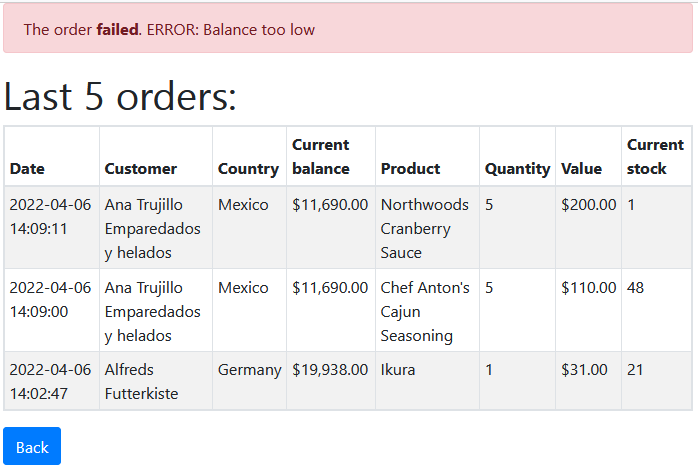
\includegraphics[width=0.75\linewidth,height=\textheight,keepaspectratio]{./images/img-082-068.png}

\begin{quote}
\textbf{MÉG TÖBB GYAKORLAT:} oszd fel a fenti táblázatot két táblára,
amelyek az utolsó 5 rendelést és az érintett ügyfelek egyenlegét külön
jelenítik meg.
\end{quote}

\textbf{Mielőtt elmész:}

\begin{enumerate}
\def\labelenumi{\arabic{enumi}.}
\tightlist
\item
  Állítsd le az alkalmazást: App engine → Settings → Disable application
\item
  Állítsd le a Postgres szervert: SQL → Overview → STOP
\item
  Kapcsold le a GCP-projektet.
\end{enumerate}

\begin{center}\rule{0.5\linewidth}{0.5pt}\end{center}

\subsection{BigQuery áttekintés és
bemutató}\label{bigquery-uxe1ttekintuxe9s-uxe9s-bemutatuxf3}

„A BigQuery standard SQL segítségével strukturált és félig strukturált
adatok lekérdezésére lett tervezve.''\footnote{Lásd:
  https://panoply.io/data-warehouse-guide/bigquery-architecture/}

A BigQuery denormalizált (ellapított) adattárházi táblákon futtatandó
\textbf{csak olvasható} OLAP-jellegű lekérdezésekre lett tervezve
döntéstámogatási és üzleti elemzési célokra. A natív tárolási modell egy
tömörített (és opcionálisan particionált) oszloptár (neve:
Dremel).\footnote{Lásd:
  https://medium.com/google-cloud/bigquery-explained-storage-overview-70cac32251fa}
Az összes adat titkosított formában tárolódik. A BigQuery közvetlenül
futtathat lekérdezéseket más adatforrásokon is, mint például Bigtable,
Cloud storage vagy Google Drive --- de a legjobb teljesítmény érdekében
az ilyen külső forrásokból származó adatokat először érdemes importálni
a Dremel oszloptárba.

A logikai adatmodell egy adatkészlet (Dataset), amely kapcsolódó
táblákat tartalmaz rögzített sémával és típusos mezőkkel; hivatkozása:
\texttt{project.dataset.table}

\subsubsection{A Northwind adatbázis
bányászata}\label{a-northwind-adatbuxe1zis-buxe1nyuxe1szata}

Ebben a demóban:

\begin{itemize}
\tightlist
\item
  Az SQL Server verzióját a Northwind adatbázisnak használjuk
\item
  Létrehozunk egy denormalizált nézetet, és exportáljuk CSV-be
\item
  Betöltjük a CSV-t egy BigQuery táblába
\item
  A táblát felhasználjuk egy lineáris regressziós BigQueryML modell
  létrehozásához
\item
  Értékeljük a modell pontosságát
\end{itemize}

Lépések:

\begin{enumerate}
\def\labelenumi{\arabic{enumi}.}
\item
  Hozz létre egy nézetet, amely a következő mezőket tartalmazza:
  \texttt{value\_numeric}, \texttt{country}, \texttt{categoryid},
  \texttt{p\_unitprice}, \texttt{discount}, \texttt{pyear}
\item
  Exportáld a nézetet CSV-fájlba.
\item
  Chrome böngészőt használva hozz létre egy új projektet: GCP főmenü →
  IAM\&admin → Manage resources.
\item
  GCP főmenü → Analytics → BigQuery, Enable API.
\item
  A projekt „\ldots'' menüjéből → Create dataset, válaszd a Multi-region
  `US' lehetőséget. Meg kell adnod egy azonosítót. Nevezd el az
  adatkészletet `northwind'-nek. Az adatkészlet titkosított formában
  kerül tárolásra. Lépj az adatkészletre.
\item
  Válaszd a + create table lehetőséget, és add meg: Create table from
  upload → schema auto-detect. Töltsd be a denormalizált táblát, és
  ellenőrizd az adattípusokat. Nevezd el a táblát `nw'-nek. A money
  (pénz) típus problémát okozhat.
\item
  Tekintsd át a sémát és az adatok előnézetét.
\item
  Érdemes ellenőrizni a forrásadatok érvényességét és tartalmát elemzés
  előtt. A GCP Analytics → Dataplex szolgáltatás ezt támogatja:

  \begin{itemize}
  \tightlist
  \item
    \begin{enumerate}
    \def\labelenumii{\alph{enumii}.}
    \tightlist
    \item
      A Dataplex-ből vagy közvetlenül a BigQuery Studióból (a Schema fül
      melletti utolsó fül) hozz létre és indíts el egy igény szerinti
      Profile task feladatot a Quick data profile → Details menüponton.
      Ez a feladat kb. 5 percig fut a háttérben, majd megjeleníti az
      oszlopstatisztikákat és hisztogramokat.
    \end{enumerate}
  \item
    \begin{enumerate}
    \def\labelenumii{\alph{enumii}.}
    \setcounter{enumii}{1}
    \tightlist
    \item
      Indíts el egy Data quality scan feladatot is egy manuálisan
      hozzáadott minőségi szabállyal (pl. Freight \textgreater=0). A
      profil feladat eredménye alapján a `de facto' szabályokat is
      áttekintheted és elfogadhatod (pl. a Freight mezőre levezetett
      szabály: ``min: 0.02, max:1007.64''). Az ellenőrzéssel kapcsolatos
      adminisztratív adatok a Northwind adatkészletben tárolhatók. Az
      eredmények a Dataplex → Data quality oldalon az ellenőrzés nevére
      kattintva, a Jobs history fülön érhetők el.
    \end{enumerate}
  \end{itemize}
\item
  A BigQuery-ben SQL lekérdezések futtathatók a konzolon: Compose new
  query → SQL console window.
\item
  Hozd létre azt a modellt, amely a \texttt{value\_numeric} mezőt
  becsüli a \texttt{country}, \texttt{categoryid},
  \texttt{p\_unitprice}, \texttt{discount}, \texttt{pyear} mezők alapján
  (ha az adatkészletet `northwind'-nek és a táblát `nw'-nek nevezted
  el):\footnote{Lásd:
    https://cloud.google.com/bigquery-ml/docs/reference/standard-sql/bigqueryml-syntax-create}
\end{enumerate}

\begin{Shaded}
\begin{Highlighting}[]
\KeywordTok{CREATE}\NormalTok{ MODEL \textasciigrave{}northwind.nw\_model\textasciigrave{} OPTIONS (model\_type}\OperatorTok{=}\StringTok{\textquotesingle{}linear\_reg\textquotesingle{}}\NormalTok{, input\_label\_cols}\OperatorTok{=}\NormalTok{[}\StringTok{\textquotesingle{}value\_numeric\textquotesingle{}}\NormalTok{]) }\KeywordTok{AS}
\KeywordTok{SELECT}\NormalTok{ value\_numeric, country, categoryid, p\_unitprice, discount, pyear}
\KeywordTok{FROM}\NormalTok{ \textasciigrave{}northwind.nw\textasciigrave{}}
\KeywordTok{WHERE}\NormalTok{ value\_numeric }\KeywordTok{is} \KeywordTok{not} \KeywordTok{null}
\end{Highlighting}
\end{Shaded}

\begin{enumerate}
\def\labelenumi{\arabic{enumi}.}
\setcounter{enumi}{10}
\item
  Épitsd fel a \texttt{northwind.nw\_model} modellt (kb. 30 másodperc),
  majd lépj a modelre. Ellenőrizd a Details és Evaluation füleket.
  Látható, hogy az adatkészlet automatikusan felosztásra kerül egy
  tanuló táblára (1702 rekord) és egy kiértékelő táblára (453 rekord).
  Az átlagos abszolút hiba 301.
\item
  A modellt a teljes adatkészlettel is kiértékelhetjük (bár ez
  adattudományos szempontból nem ajánlott bevált gyakorlat --- csak az
  EVALUATE módszer bemutatása céljából tesszük). Használd a következő
  parancsot:
\end{enumerate}

\begin{Shaded}
\begin{Highlighting}[]
\KeywordTok{SELECT} \OperatorTok{*} \KeywordTok{FROM}\NormalTok{ ML.EVALUATE(MODEL \textasciigrave{}northwind.nw\_model\textasciigrave{}, (}
 \KeywordTok{SELECT}\NormalTok{ value\_numeric, country, categoryid, p\_unitprice, discount, pyear}
 \KeywordTok{FROM}\NormalTok{ \textasciigrave{}northwind.nw\textasciigrave{}}
\NormalTok{))}
\end{Highlighting}
\end{Shaded}

\begin{enumerate}
\def\labelenumi{\arabic{enumi}.}
\setcounter{enumi}{12}
\tightlist
\item
  Az eredmények azt mutatják, hogy az előrejelzés átlagos hibája 342, a
  magyarázott variancia 53\%, tehát a modell teljesítménye gyenge: a
  függő változó és a független változók közötti kapcsolat gyenge. Ha
  újra létrehozzuk a modellt a \texttt{CALCULATE\_P\_VALUES\ =\ true},
  \texttt{CATEGORY\_ENCODING\_METHOD=\textquotesingle{}DUMMY\_ENCODING\textquotesingle{}}
  opciókkal, ellenőrizhetjük, hogy az egyes változók hozzájárulása
  szignifikáns-e.\footnote{Úgy tűnik, ez a funkció jelenleg nem működik.}
  Azokat a rekordokat, ahol a hiba kisebb volt 40\%-nál, a következő
  paranccsal kérdezhetjük le. Hasonlóképpen megállapítható, hogy a
  legrosszabb előrejelzés 17,0 helyett 517,9 volt.
\end{enumerate}

\begin{Shaded}
\begin{Highlighting}[]
\KeywordTok{SELECT} \OperatorTok{*} \KeywordTok{FROM}\NormalTok{ ML.PREDICT(MODEL \textasciigrave{}northwind.nw\_model\textasciigrave{}, (}
 \KeywordTok{SELECT}\NormalTok{ value\_numeric, country, categoryid, p\_unitprice, discount, pyear}
 \KeywordTok{FROM}\NormalTok{ \textasciigrave{}northwind.nw\textasciigrave{}}
\NormalTok{)) }\KeywordTok{where} \FunctionTok{abs}\NormalTok{((predicted\_value\_numeric}\OperatorTok{{-}}\NormalTok{value\_numeric))}\OperatorTok{/}\NormalTok{value\_numeric}\OperatorTok{\textless{}}\FloatTok{0.4}
\end{Highlighting}
\end{Shaded}

\begin{quote}
\textbf{GYAKORLAT:} módosítsd a nézetet úgy, hogy tartalmazza a
\texttt{value\_nominal} mezőt, amely három kategóriát tartalmaz az
alacsony, közepes és magas árú tételekhez. Próbáld meg a
\texttt{value\_nominal} mezőt a \texttt{BOOSTED\_TREE\_CLASSIFIER} vagy
a \texttt{LOGISTIC\_REG} módszerrel becsülni. Hány esetben/milyen
százalékban tudod helyesen megbecsülni az osztálycímkét?

Segítség:

\begin{Shaded}
\begin{Highlighting}[]
\KeywordTok{select}\NormalTok{ od.unitprice}\OperatorTok{*}\NormalTok{od.quantity}\OperatorTok{*}\NormalTok{(}\DecValTok{1}\OperatorTok{{-}}\NormalTok{od.discount) }\FunctionTok{value}\NormalTok{,}
\ControlFlowTok{case} \ControlFlowTok{when}\NormalTok{ (od.unitprice}\OperatorTok{*}\NormalTok{od.quantity}\OperatorTok{*}\NormalTok{(}\DecValTok{1}\OperatorTok{{-}}\NormalTok{od.discount)) }\OperatorTok{\textless{}} \DecValTok{200} \ControlFlowTok{then} \StringTok{\textquotesingle{}L\textquotesingle{}}
      \ControlFlowTok{when}\NormalTok{ (od.unitprice}\OperatorTok{*}\NormalTok{od.quantity}\OperatorTok{*}\NormalTok{(}\DecValTok{1}\OperatorTok{{-}}\NormalTok{od.discount)) }\OperatorTok{\textless{}} \DecValTok{1200} \ControlFlowTok{then} \StringTok{\textquotesingle{}M\textquotesingle{}}
      \ControlFlowTok{when}\NormalTok{ (od.unitprice}\OperatorTok{*}\NormalTok{od.quantity}\OperatorTok{*}\NormalTok{(}\DecValTok{1}\OperatorTok{{-}}\NormalTok{od.discount)) }\OperatorTok{\textgreater{}=} \DecValTok{1200} \ControlFlowTok{then} \StringTok{\textquotesingle{}H\textquotesingle{}}
\ControlFlowTok{else} \StringTok{\textquotesingle{}N/A\textquotesingle{}} \ControlFlowTok{end}\NormalTok{ value\_nominal,}
\NormalTok{c.CustomerID, c.CompanyName, c.Country, c.Balance, o.OrderID,  o.OrderDate, o.RequiredDate,}
\DataTypeTok{year}\NormalTok{(o.orderdate) pyear,}
\NormalTok{o.ShippedDate, o.ShipVia, o.Freight, o.ShipName, o.ShipAddress, o.ShipCity, o.ShipRegion,}
\NormalTok{o.ShipPostalCode, o.ShipCountry, od.UnitPrice, od.Quantity, od.Discount,}
\NormalTok{p.ProductName, p.SupplierID, p.CategoryID,}
\NormalTok{p.QuantityPerUnit, p.UnitPrice p\_unitprice, p.UnitsInStock, p.UnitsOnOrder, p.ReorderLevel,}
\NormalTok{p.Discontinued}
\KeywordTok{from}\NormalTok{ Customers }\KeywordTok{AS}\NormalTok{ c }\KeywordTok{join}\NormalTok{ Orders }\KeywordTok{AS}\NormalTok{ o }\KeywordTok{ON}\NormalTok{ c.CustomerID }\OperatorTok{=}\NormalTok{ o.CustomerID }\KeywordTok{join}
\NormalTok{[}\KeywordTok{Order}\NormalTok{ Details] }\KeywordTok{AS}\NormalTok{ od }\KeywordTok{ON}\NormalTok{ o.OrderID }\OperatorTok{=}\NormalTok{ od.OrderID }\KeywordTok{join}
\NormalTok{Products }\KeywordTok{AS}\NormalTok{ p }\KeywordTok{ON}\NormalTok{ od.ProductID }\OperatorTok{=}\NormalTok{ p.ProductID}
\end{Highlighting}
\end{Shaded}
\end{quote}

\begin{quote}
\textbf{GYAKORLAT:} használd a nyilvános
\texttt{bigquery-public-data.samples.natality}\footnote{Lásd:
  https://cloud.google.com/bigquery-ml/docs/bigqueryml-natality} teszt
táblát egy csecsemő születési súlyának becslésére lineáris
regresszióval. Ez a tábla sok rekordot tartalmaz, ezért mintát vehetsz
belőle egy \texttt{WHERE\ RAND()\ \textless{}\ 0.0001} feltétellel.

Segítség:

Ha az adatkészleted nem az US régióban lett létrehozva, hozz létre egy
új adatkészletet `US' Multi-régióban \texttt{us\_dataset} névvel, majd
futtasd az alábbi lekérdezést --- így nem kell manuálisan beállítanod a
lekérdezés régióját (a MORE → Query settings → Advanced options
menüben):

\begin{Shaded}
\begin{Highlighting}[]
\KeywordTok{CREATE}\NormalTok{ MODEL \textasciigrave{}us\_dataset.natality\_model\textasciigrave{}}
\NormalTok{OPTIONS}
\NormalTok{  (model\_type}\OperatorTok{=}\StringTok{\textquotesingle{}linear\_reg\textquotesingle{}}\NormalTok{,}
\NormalTok{    input\_label\_cols}\OperatorTok{=}\NormalTok{[}\StringTok{\textquotesingle{}weight\_pounds\textquotesingle{}}\NormalTok{]) }\KeywordTok{AS}
\KeywordTok{SELECT}
\NormalTok{  weight\_pounds,}
\NormalTok{  is\_male,}
\NormalTok{  gestation\_weeks,}
\NormalTok{  mother\_age,}
  \FunctionTok{CAST}\NormalTok{(mother\_race }\KeywordTok{AS}\NormalTok{ string) }\KeywordTok{AS}\NormalTok{ mother\_race}
\KeywordTok{FROM}
\NormalTok{  \textasciigrave{}bigquery}\OperatorTok{{-}}\KeywordTok{public}\OperatorTok{{-}}\KeywordTok{data}\NormalTok{.samples.natality\textasciigrave{}}
\KeywordTok{WHERE}
\NormalTok{  weight\_pounds }\KeywordTok{IS} \KeywordTok{NOT} \KeywordTok{NULL} \KeywordTok{AND}\NormalTok{ RAND() }\OperatorTok{\textless{}} \FloatTok{0.0001}

\KeywordTok{SELECT}  \OperatorTok{*} \KeywordTok{FROM}\NormalTok{  ML.TRAINING\_INFO(MODEL \textasciigrave{}dataset\_nev.natality\_model\textasciigrave{})}

\KeywordTok{SELECT} \OperatorTok{*} \KeywordTok{FROM}\NormalTok{ ML.PREDICT(MODEL \textasciigrave{}dataset\_nev.natality\_model\textasciigrave{},}
\NormalTok{(}\KeywordTok{select} \KeywordTok{true} \KeywordTok{as}\NormalTok{ is\_male, }\DecValTok{40} \KeywordTok{as}\NormalTok{ gestation\_weeks, }\DecValTok{30} \KeywordTok{as}\NormalTok{ mother\_age,}\StringTok{\textquotesingle{}38\textquotesingle{}} \KeywordTok{as}\NormalTok{ mother\_race))}
\end{Highlighting}
\end{Shaded}
\end{quote}

\begin{center}\rule{0.5\linewidth}{0.5pt}\end{center}

\subsection{További olvasnivaló}\label{tovuxe1bbi-olvasnivaluxf3}

\begin{itemize}
\tightlist
\item
  Faculty training: https://edu.google.com/programs/faculty/training
\item
  Learning paths: https://cloud.google.com/training
\item
  Quickstarts (rövid oktatóanyagok a Cloud Platform termékekhez,
  szolgáltatásokhoz és API-khoz):
  https://cloud.google.com/gcp/getting-started
\item
  Sample Projects: https://go.google-mkto.com/CPI00b01C3FT0A2j1tciC0V
\item
  GCP docs: https://cloud.google.com/docs
\end{itemize}

\begin{center}\rule{0.5\linewidth}{0.5pt}\end{center}

\section{8. Gráfmodellek és
BLOB-tárolás}\label{gruxe1fmodellek-uxe9s-blob-tuxe1roluxe1s}

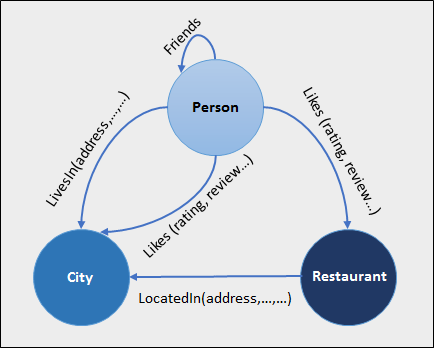
\includegraphics[width=0.75\linewidth,height=\textheight,keepaspectratio]{./images/img-087-069.png}

Az UML- és ERM-modellek az entitásokat és azok kapcsolatait írják le. A
szokásos megközelítés szerint ezekből relációs modell készül. A
\textbf{gráfmodell} (graph model) a csomópontokat --- a gráfelméletben:
\textbf{csúcsokat} (nodes) --- és az éleket (edges) helyezi a
középpontba; alternatívát kínál a relációs modellhez, és bizonyos
lekérdezéseknél (pl. hálózati bejárás, legrövidebb út) hatékonyabb
lehet. (A kurzus végig a Microsoft SQL Server-dokumentációban használt
„csomópont'' kifejezést alkalmazza, de az „él'' és a „kapcsolat'' nem
szinonimák: az él strukturális kapcsolat a gráfban, a kapcsolat pedig a
kapcsolat szemantikai jelentése.)

\begin{center}\rule{0.5\linewidth}{0.5pt}\end{center}

\subsection{SQL Server gráftáblák}\label{sql-server-gruxe1ftuxe1bluxe1k}

Az SQL Server 2017-től natív gráftábla-támogatással rendelkezik. A
legfontosabb fogalmak:

\begin{itemize}
\tightlist
\item
  \textbf{Csomóponttábla} (Node table): \texttt{AS\ NODE} záradékkal
  hozható létre; a tábla sorai a gráf csomópontjait képviselik
\item
  \textbf{Éltábla} (Edge table): \texttt{AS\ EDGE} záradékkal hozható
  létre; a tábla sorai az irányított éleket képviselik
\item
  \textbf{\texttt{\$node\_id}}: a csomópontok rendszer által generált
  belső azonosítója (pszeudo-oszlop)
\item
  \textbf{\texttt{\$edge\_id}}: az élek rendszer által generált belső
  azonosítója (pszeudo-oszlop)
\item
  \textbf{\texttt{MATCH}}: kulcsszó gráf-mintaillesztéses
  lekérdezésekhez; a \texttt{-(él)-\textgreater{}} szintaxis irányított
  élt jelöl
\end{itemize}

\begin{quote}
\textbf{DEMO:} hozz létre egy közösségi hálózatot modellező
gráf-adatbázist.
\end{quote}

\begin{Shaded}
\begin{Highlighting}[]
\KeywordTok{use} \KeywordTok{master}
\NormalTok{go}
\KeywordTok{create} \KeywordTok{database}\NormalTok{ graphdemo}
\NormalTok{go}
\KeywordTok{use}\NormalTok{ graphdemo}
\NormalTok{go}

\CommentTok{{-}{-} Csomóponttáblák}
\KeywordTok{create} \KeywordTok{table}\NormalTok{ person (}\KeywordTok{id} \DataTypeTok{integer}\NormalTok{, name }\DataTypeTok{varchar}\NormalTok{(}\DecValTok{100}\NormalTok{)) }\KeywordTok{as}\NormalTok{ node;}
\KeywordTok{create} \KeywordTok{table}\NormalTok{ restaurant (}\KeywordTok{id} \DataTypeTok{integer}\NormalTok{, name }\DataTypeTok{varchar}\NormalTok{(}\DecValTok{100}\NormalTok{), city }\DataTypeTok{varchar}\NormalTok{(}\DecValTok{100}\NormalTok{)) }\KeywordTok{as}\NormalTok{ node;}
\KeywordTok{create} \KeywordTok{table}\NormalTok{ city (}\KeywordTok{id} \DataTypeTok{integer}\NormalTok{, name }\DataTypeTok{varchar}\NormalTok{(}\DecValTok{100}\NormalTok{)) }\KeywordTok{as}\NormalTok{ node;}

\CommentTok{{-}{-} Éltáblák}
\KeywordTok{create} \KeywordTok{table}\NormalTok{ likes }\KeywordTok{as}\NormalTok{ edge;}
\KeywordTok{create} \KeywordTok{table}\NormalTok{ friendof }\KeywordTok{as}\NormalTok{ edge;}
\KeywordTok{create} \KeywordTok{table}\NormalTok{ livesin }\KeywordTok{as}\NormalTok{ edge;}
\KeywordTok{create} \KeywordTok{table}\NormalTok{ locatedin }\KeywordTok{as}\NormalTok{ edge;}

\CommentTok{{-}{-} Személyek}
\KeywordTok{insert} \KeywordTok{into}\NormalTok{ person }\KeywordTok{values}\NormalTok{ (}\DecValTok{1}\NormalTok{, }\StringTok{\textquotesingle{}john\textquotesingle{}}\NormalTok{);}
\KeywordTok{insert} \KeywordTok{into}\NormalTok{ person }\KeywordTok{values}\NormalTok{ (}\DecValTok{2}\NormalTok{, }\StringTok{\textquotesingle{}mary\textquotesingle{}}\NormalTok{);}
\KeywordTok{insert} \KeywordTok{into}\NormalTok{ person }\KeywordTok{values}\NormalTok{ (}\DecValTok{3}\NormalTok{, }\StringTok{\textquotesingle{}alice\textquotesingle{}}\NormalTok{);}
\KeywordTok{insert} \KeywordTok{into}\NormalTok{ person }\KeywordTok{values}\NormalTok{ (}\DecValTok{4}\NormalTok{, }\StringTok{\textquotesingle{}peter\textquotesingle{}}\NormalTok{);}

\CommentTok{{-}{-} Városok}
\KeywordTok{insert} \KeywordTok{into}\NormalTok{ city }\KeywordTok{values}\NormalTok{ (}\DecValTok{1}\NormalTok{, }\StringTok{\textquotesingle{}New York\textquotesingle{}}\NormalTok{);}
\KeywordTok{insert} \KeywordTok{into}\NormalTok{ city }\KeywordTok{values}\NormalTok{ (}\DecValTok{2}\NormalTok{, }\StringTok{\textquotesingle{}London\textquotesingle{}}\NormalTok{);}

\CommentTok{{-}{-} Éttermek}
\KeywordTok{insert} \KeywordTok{into}\NormalTok{ restaurant }\KeywordTok{values}\NormalTok{ (}\DecValTok{1}\NormalTok{, }\StringTok{\textquotesingle{}Ristorante Rosso\textquotesingle{}}\NormalTok{, }\StringTok{\textquotesingle{}New York\textquotesingle{}}\NormalTok{);}
\KeywordTok{insert} \KeywordTok{into}\NormalTok{ restaurant }\KeywordTok{values}\NormalTok{ (}\DecValTok{2}\NormalTok{, }\StringTok{\textquotesingle{}Trattoria Verde\textquotesingle{}}\NormalTok{, }\StringTok{\textquotesingle{}London\textquotesingle{}}\NormalTok{);}
\KeywordTok{insert} \KeywordTok{into}\NormalTok{ restaurant }\KeywordTok{values}\NormalTok{ (}\DecValTok{3}\NormalTok{, }\StringTok{\textquotesingle{}Café Bleu\textquotesingle{}}\NormalTok{, }\StringTok{\textquotesingle{}New York\textquotesingle{}}\NormalTok{);}

\CommentTok{{-}{-} Barátság{-}élek ($node\_id alapján)}
\KeywordTok{insert} \KeywordTok{into}\NormalTok{ friendof }\KeywordTok{values}
\NormalTok{ ((}\KeywordTok{select}\NormalTok{ $node\_id }\KeywordTok{from}\NormalTok{ person }\KeywordTok{where}\NormalTok{ name }\OperatorTok{=} \StringTok{\textquotesingle{}john\textquotesingle{}}\NormalTok{),}
\NormalTok{ (}\KeywordTok{select}\NormalTok{ $node\_id }\KeywordTok{from}\NormalTok{ person }\KeywordTok{where}\NormalTok{ name }\OperatorTok{=} \StringTok{\textquotesingle{}mary\textquotesingle{}}\NormalTok{));}
\KeywordTok{insert} \KeywordTok{into}\NormalTok{ friendof }\KeywordTok{values}
\NormalTok{ ((}\KeywordTok{select}\NormalTok{ $node\_id }\KeywordTok{from}\NormalTok{ person }\KeywordTok{where}\NormalTok{ name }\OperatorTok{=} \StringTok{\textquotesingle{}john\textquotesingle{}}\NormalTok{),}
\NormalTok{ (}\KeywordTok{select}\NormalTok{ $node\_id }\KeywordTok{from}\NormalTok{ person }\KeywordTok{where}\NormalTok{ name }\OperatorTok{=} \StringTok{\textquotesingle{}alice\textquotesingle{}}\NormalTok{));}
\KeywordTok{insert} \KeywordTok{into}\NormalTok{ friendof }\KeywordTok{values}
\NormalTok{ ((}\KeywordTok{select}\NormalTok{ $node\_id }\KeywordTok{from}\NormalTok{ person }\KeywordTok{where}\NormalTok{ name }\OperatorTok{=} \StringTok{\textquotesingle{}mary\textquotesingle{}}\NormalTok{),}
\NormalTok{ (}\KeywordTok{select}\NormalTok{ $node\_id }\KeywordTok{from}\NormalTok{ person }\KeywordTok{where}\NormalTok{ name }\OperatorTok{=} \StringTok{\textquotesingle{}peter\textquotesingle{}}\NormalTok{));}

\CommentTok{{-}{-} Tetszik{-}élek}
\KeywordTok{insert} \KeywordTok{into}\NormalTok{ likes }\KeywordTok{values}
\NormalTok{ ((}\KeywordTok{select}\NormalTok{ $node\_id }\KeywordTok{from}\NormalTok{ person }\KeywordTok{where}\NormalTok{ name }\OperatorTok{=} \StringTok{\textquotesingle{}john\textquotesingle{}}\NormalTok{),}
\NormalTok{ (}\KeywordTok{select}\NormalTok{ $node\_id }\KeywordTok{from}\NormalTok{ restaurant }\KeywordTok{where}\NormalTok{ name }\OperatorTok{=} \StringTok{\textquotesingle{}Ristorante Rosso\textquotesingle{}}\NormalTok{));}
\KeywordTok{insert} \KeywordTok{into}\NormalTok{ likes }\KeywordTok{values}
\NormalTok{ ((}\KeywordTok{select}\NormalTok{ $node\_id }\KeywordTok{from}\NormalTok{ person }\KeywordTok{where}\NormalTok{ name }\OperatorTok{=} \StringTok{\textquotesingle{}mary\textquotesingle{}}\NormalTok{),}
\NormalTok{ (}\KeywordTok{select}\NormalTok{ $node\_id }\KeywordTok{from}\NormalTok{ restaurant }\KeywordTok{where}\NormalTok{ name }\OperatorTok{=} \StringTok{\textquotesingle{}Ristorante Rosso\textquotesingle{}}\NormalTok{));}
\KeywordTok{insert} \KeywordTok{into}\NormalTok{ likes }\KeywordTok{values}
\NormalTok{ ((}\KeywordTok{select}\NormalTok{ $node\_id }\KeywordTok{from}\NormalTok{ person }\KeywordTok{where}\NormalTok{ name }\OperatorTok{=} \StringTok{\textquotesingle{}alice\textquotesingle{}}\NormalTok{),}
\NormalTok{ (}\KeywordTok{select}\NormalTok{ $node\_id }\KeywordTok{from}\NormalTok{ restaurant }\KeywordTok{where}\NormalTok{ name }\OperatorTok{=} \StringTok{\textquotesingle{}Trattoria Verde\textquotesingle{}}\NormalTok{));}

\CommentTok{{-}{-} Lakóhely{-}élek}
\KeywordTok{insert} \KeywordTok{into}\NormalTok{ livesin }\KeywordTok{values}
\NormalTok{ ((}\KeywordTok{select}\NormalTok{ $node\_id }\KeywordTok{from}\NormalTok{ person }\KeywordTok{where}\NormalTok{ name }\OperatorTok{=} \StringTok{\textquotesingle{}john\textquotesingle{}}\NormalTok{),}
\NormalTok{ (}\KeywordTok{select}\NormalTok{ $node\_id }\KeywordTok{from}\NormalTok{ city }\KeywordTok{where}\NormalTok{ name }\OperatorTok{=} \StringTok{\textquotesingle{}New York\textquotesingle{}}\NormalTok{));}
\KeywordTok{insert} \KeywordTok{into}\NormalTok{ livesin }\KeywordTok{values}
\NormalTok{ ((}\KeywordTok{select}\NormalTok{ $node\_id }\KeywordTok{from}\NormalTok{ person }\KeywordTok{where}\NormalTok{ name }\OperatorTok{=} \StringTok{\textquotesingle{}mary\textquotesingle{}}\NormalTok{),}
\NormalTok{ (}\KeywordTok{select}\NormalTok{ $node\_id }\KeywordTok{from}\NormalTok{ city }\KeywordTok{where}\NormalTok{ name }\OperatorTok{=} \StringTok{\textquotesingle{}London\textquotesingle{}}\NormalTok{));}
\KeywordTok{insert} \KeywordTok{into}\NormalTok{ livesin }\KeywordTok{values}
\NormalTok{ ((}\KeywordTok{select}\NormalTok{ $node\_id }\KeywordTok{from}\NormalTok{ person }\KeywordTok{where}\NormalTok{ name }\OperatorTok{=} \StringTok{\textquotesingle{}alice\textquotesingle{}}\NormalTok{),}
\NormalTok{ (}\KeywordTok{select}\NormalTok{ $node\_id }\KeywordTok{from}\NormalTok{ city }\KeywordTok{where}\NormalTok{ name }\OperatorTok{=} \StringTok{\textquotesingle{}London\textquotesingle{}}\NormalTok{));}
\KeywordTok{insert} \KeywordTok{into}\NormalTok{ livesin }\KeywordTok{values}
\NormalTok{ ((}\KeywordTok{select}\NormalTok{ $node\_id }\KeywordTok{from}\NormalTok{ person }\KeywordTok{where}\NormalTok{ name }\OperatorTok{=} \StringTok{\textquotesingle{}peter\textquotesingle{}}\NormalTok{),}
\NormalTok{ (}\KeywordTok{select}\NormalTok{ $node\_id }\KeywordTok{from}\NormalTok{ city }\KeywordTok{where}\NormalTok{ name }\OperatorTok{=} \StringTok{\textquotesingle{}New York\textquotesingle{}}\NormalTok{));}

\CommentTok{{-}{-} Étterem{-}elhelyezkedési élek}
\KeywordTok{insert} \KeywordTok{into}\NormalTok{ locatedin }\KeywordTok{values}
\NormalTok{ ((}\KeywordTok{select}\NormalTok{ $node\_id }\KeywordTok{from}\NormalTok{ restaurant }\KeywordTok{where}\NormalTok{ name }\OperatorTok{=} \StringTok{\textquotesingle{}Ristorante Rosso\textquotesingle{}}\NormalTok{),}
\NormalTok{ (}\KeywordTok{select}\NormalTok{ $node\_id }\KeywordTok{from}\NormalTok{ city }\KeywordTok{where}\NormalTok{ name }\OperatorTok{=} \StringTok{\textquotesingle{}New York\textquotesingle{}}\NormalTok{));}
\KeywordTok{insert} \KeywordTok{into}\NormalTok{ locatedin }\KeywordTok{values}
\NormalTok{ ((}\KeywordTok{select}\NormalTok{ $node\_id }\KeywordTok{from}\NormalTok{ restaurant }\KeywordTok{where}\NormalTok{ name }\OperatorTok{=} \StringTok{\textquotesingle{}Trattoria Verde\textquotesingle{}}\NormalTok{),}
\NormalTok{ (}\KeywordTok{select}\NormalTok{ $node\_id }\KeywordTok{from}\NormalTok{ city }\KeywordTok{where}\NormalTok{ name }\OperatorTok{=} \StringTok{\textquotesingle{}London\textquotesingle{}}\NormalTok{));}
\KeywordTok{insert} \KeywordTok{into}\NormalTok{ locatedin }\KeywordTok{values}
\NormalTok{ ((}\KeywordTok{select}\NormalTok{ $node\_id }\KeywordTok{from}\NormalTok{ restaurant }\KeywordTok{where}\NormalTok{ name }\OperatorTok{=} \StringTok{\textquotesingle{}Café Bleu\textquotesingle{}}\NormalTok{),}
\NormalTok{ (}\KeywordTok{select}\NormalTok{ $node\_id }\KeywordTok{from}\NormalTok{ city }\KeywordTok{where}\NormalTok{ name }\OperatorTok{=} \StringTok{\textquotesingle{}New York\textquotesingle{}}\NormalTok{));}
\end{Highlighting}
\end{Shaded}

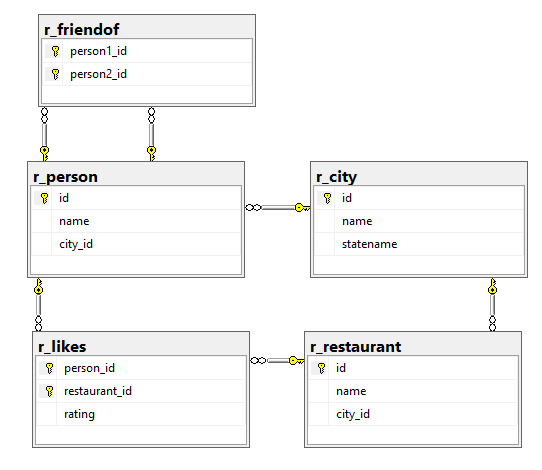
\includegraphics[width=0.75\linewidth,height=\textheight,keepaspectratio]{./images/img-091-070.png}

Gráf-mintaillesztéses lekérdezések a \texttt{MATCH} záradékkal:

\begin{Shaded}
\begin{Highlighting}[]
\CommentTok{{-}{-} John barátai}
\KeywordTok{select}\NormalTok{ p2.name}
\KeywordTok{from}\NormalTok{ person p1, friendof f, person p2}
\KeywordTok{where}\NormalTok{ match(p1}\OperatorTok{{-}}\NormalTok{(f)}\OperatorTok{{-}\textgreater{}}\NormalTok{p2)}
\KeywordTok{and}\NormalTok{ p1.name }\OperatorTok{=} \StringTok{\textquotesingle{}john\textquotesingle{}}\NormalTok{;}

\CommentTok{{-}{-} John által kedvelt éttermek}
\KeywordTok{select}\NormalTok{ r.name}
\KeywordTok{from}\NormalTok{ person p, likes l, restaurant r}
\KeywordTok{where}\NormalTok{ match(p}\OperatorTok{{-}}\NormalTok{(l)}\OperatorTok{{-}\textgreater{}}\NormalTok{r)}
\KeywordTok{and}\NormalTok{ p.name }\OperatorTok{=} \StringTok{\textquotesingle{}john\textquotesingle{}}\NormalTok{;}

\CommentTok{{-}{-} John barátai által kedvelt éttermek}
\KeywordTok{select}\NormalTok{ p2.name }\KeywordTok{as}\NormalTok{ friend, r.name }\KeywordTok{as}\NormalTok{ restaurant}
\KeywordTok{from}\NormalTok{ person p1, friendof f, person p2, likes l, restaurant r}
\KeywordTok{where}\NormalTok{ match(p1}\OperatorTok{{-}}\NormalTok{(f)}\OperatorTok{{-}\textgreater{}}\NormalTok{p2}\OperatorTok{{-}}\NormalTok{(l)}\OperatorTok{{-}\textgreater{}}\NormalTok{r)}
\KeywordTok{and}\NormalTok{ p1.name }\OperatorTok{=} \StringTok{\textquotesingle{}john\textquotesingle{}}\NormalTok{;}

\CommentTok{{-}{-} Azonos városban lakó személyek}
\KeywordTok{select}\NormalTok{ p1.name, p2.name}
\KeywordTok{from}\NormalTok{ person p1, livesin l1, city c, livesin l2, person p2}
\KeywordTok{where}\NormalTok{ match(p1}\OperatorTok{{-}}\NormalTok{(l1)}\OperatorTok{{-}\textgreater{}}\NormalTok{c}\OperatorTok{\textless{}{-}}\NormalTok{(l2)}\OperatorTok{{-}}\NormalTok{p2)}
\KeywordTok{and}\NormalTok{ p1.name }\OperatorTok{\textless{}\textgreater{}}\NormalTok{ p2.name;}
\end{Highlighting}
\end{Shaded}

\subsubsection{SHORTEST\_PATH (SQL Server
2019+)}\label{shortest_path-sql-server-2019}

\begin{Shaded}
\begin{Highlighting}[]
\KeywordTok{select}\NormalTok{ p1.name,}
\NormalTok{   string\_agg(p2.name, }\StringTok{\textquotesingle{}{-}\textgreater{}\textquotesingle{}}\NormalTok{) within }\KeywordTok{group}\NormalTok{ (graph path) }\KeywordTok{as}\NormalTok{ path,}
   \FunctionTok{count}\NormalTok{(p2.name) within }\KeywordTok{group}\NormalTok{ (graph path) }\KeywordTok{as}\NormalTok{ path\_length}
\KeywordTok{from}\NormalTok{ person p1,}
\NormalTok{  friendof }\ControlFlowTok{for}\NormalTok{ path fo,}
\NormalTok{  person }\ControlFlowTok{for}\NormalTok{ path p2}
\KeywordTok{where}\NormalTok{ match(shortest\_path(p1(}\OperatorTok{{-}}\NormalTok{(fo)}\OperatorTok{{-}\textgreater{}}\NormalTok{p2)}\OperatorTok{+}\NormalTok{))}
\KeywordTok{and}\NormalTok{ p1.name }\OperatorTok{=} \StringTok{\textquotesingle{}john\textquotesingle{}}\NormalTok{;}
\end{Highlighting}
\end{Shaded}

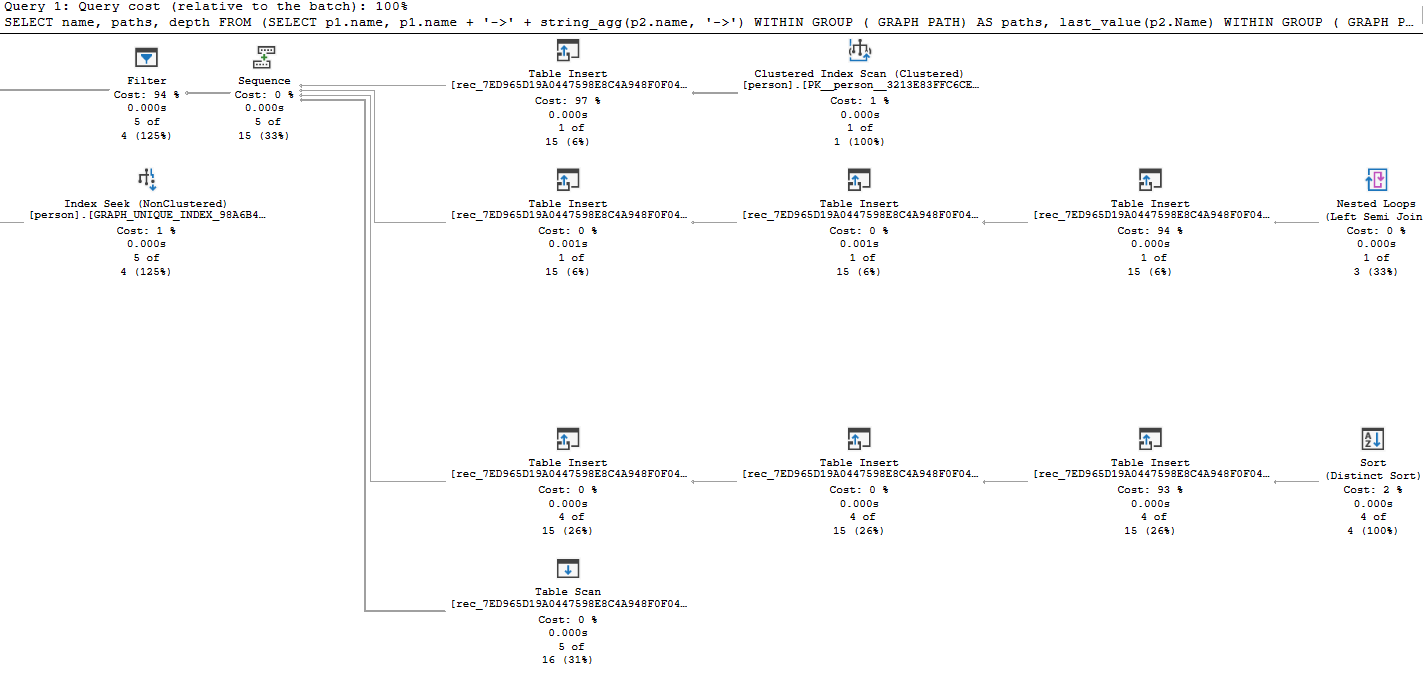
\includegraphics[width=0.75\linewidth,height=\textheight,keepaspectratio]{./images/img-093-071.png}

\subsubsection{Hagyományos relációs
megfelelő}\label{hagyomuxe1nyos-reluxe1ciuxf3s-megfelelux151}

Ugyanez a modell öt relációs táblával is megvalósítható:

\begin{Shaded}
\begin{Highlighting}[]
\KeywordTok{create} \KeywordTok{table}\NormalTok{ r\_person (}\KeywordTok{id} \DataTypeTok{integer} \KeywordTok{primary} \KeywordTok{key}\NormalTok{, name }\DataTypeTok{varchar}\NormalTok{(}\DecValTok{100}\NormalTok{));}
\KeywordTok{create} \KeywordTok{table}\NormalTok{ r\_city (}\KeywordTok{id} \DataTypeTok{integer} \KeywordTok{primary} \KeywordTok{key}\NormalTok{, name }\DataTypeTok{varchar}\NormalTok{(}\DecValTok{100}\NormalTok{));}
\KeywordTok{create} \KeywordTok{table}\NormalTok{ r\_restaurant (}\KeywordTok{id} \DataTypeTok{integer} \KeywordTok{primary} \KeywordTok{key}\NormalTok{, name }\DataTypeTok{varchar}\NormalTok{(}\DecValTok{100}\NormalTok{),}
\NormalTok{ city\_id }\DataTypeTok{integer} \KeywordTok{references}\NormalTok{ r\_city(}\KeywordTok{id}\NormalTok{));}
\KeywordTok{create} \KeywordTok{table}\NormalTok{ r\_likes (person\_id }\DataTypeTok{integer} \KeywordTok{references}\NormalTok{ r\_person(}\KeywordTok{id}\NormalTok{),}
\NormalTok{ restaurant\_id }\DataTypeTok{integer} \KeywordTok{references}\NormalTok{ r\_restaurant(}\KeywordTok{id}\NormalTok{));}
\KeywordTok{create} \KeywordTok{table}\NormalTok{ r\_friendof (person\_id }\DataTypeTok{integer} \KeywordTok{references}\NormalTok{ r\_person(}\KeywordTok{id}\NormalTok{),}
\NormalTok{ friend\_id }\DataTypeTok{integer} \KeywordTok{references}\NormalTok{ r\_person(}\KeywordTok{id}\NormalTok{));}
\end{Highlighting}
\end{Shaded}

Relációs sémával a bejárások több JOIN-t igényelnek --- pl. „John
barátainak barátai által kedvelt éttermek'' négy JOIN-t kíván. A
gráftáblás megközelítés olvashatóbb és természetesebb az ilyen
lekérdezéstípusoknál.

\begin{quote}
\textbf{GYAKORLAT:}

\begin{enumerate}
\def\labelenumi{\arabic{enumi}.}
\tightlist
\item
  Valósítsd meg az Orders / Order Details / Products táblakapcsolatokat
  gráfként az AdventureworksDW2019 adatbázisban, és futtass
  MATCH-lekérdezéseket.
\item
  Futtasd az alábbi T-SQL szkriptet, amely véletlenszerű gráfot generál
  100 csomóponttal és 300 éllel, majd mérd meg az átmérőt (a leghosszabb
  legrövidebb út hosszát) \texttt{SHORTEST\_PATH} segítségével.
\end{enumerate}
\end{quote}

\begin{Shaded}
\begin{Highlighting}[]
\CommentTok{{-}{-} Véletlenszerű gráf generálása}
\KeywordTok{drop} \KeywordTok{table} \ControlFlowTok{if} \KeywordTok{exists}\NormalTok{ rnd\_edge;}
\KeywordTok{drop} \KeywordTok{table} \ControlFlowTok{if} \KeywordTok{exists}\NormalTok{ rnd\_node;}
\KeywordTok{create} \KeywordTok{table}\NormalTok{ rnd\_node (}\KeywordTok{id} \DataTypeTok{integer}\NormalTok{) }\KeywordTok{as}\NormalTok{ node;}
\KeywordTok{create} \KeywordTok{table}\NormalTok{ rnd\_edge }\KeywordTok{as}\NormalTok{ edge;}

\KeywordTok{declare}\NormalTok{ @i }\DataTypeTok{integer} \OperatorTok{=} \DecValTok{0}\NormalTok{;}
\ControlFlowTok{while}\NormalTok{ @i }\OperatorTok{\textless{}} \DecValTok{100}
\ControlFlowTok{begin}
 \KeywordTok{insert} \KeywordTok{into}\NormalTok{ rnd\_node }\KeywordTok{values}\NormalTok{ (@i);}
 \KeywordTok{set}\NormalTok{ @i }\OperatorTok{=}\NormalTok{ @i }\OperatorTok{+} \DecValTok{1}\NormalTok{;}
\ControlFlowTok{end}\NormalTok{;}

\KeywordTok{declare}\NormalTok{ @j }\DataTypeTok{integer} \OperatorTok{=} \DecValTok{0}\NormalTok{;}
\ControlFlowTok{while}\NormalTok{ @j }\OperatorTok{\textless{}} \DecValTok{300}
\ControlFlowTok{begin}
 \KeywordTok{insert} \KeywordTok{into}\NormalTok{ rnd\_edge }\KeywordTok{values}\NormalTok{ (}
\NormalTok{  (}\KeywordTok{select}\NormalTok{ $node\_id }\KeywordTok{from}\NormalTok{ rnd\_node }\KeywordTok{where} \KeywordTok{id} \OperatorTok{=} \FunctionTok{abs}\NormalTok{(checksum(newid())) \% }\DecValTok{100}\NormalTok{),}
\NormalTok{  (}\KeywordTok{select}\NormalTok{ $node\_id }\KeywordTok{from}\NormalTok{ rnd\_node }\KeywordTok{where} \KeywordTok{id} \OperatorTok{=} \FunctionTok{abs}\NormalTok{(checksum(newid())) \% }\DecValTok{100}\NormalTok{)}
\NormalTok{ );}
 \KeywordTok{set}\NormalTok{ @j }\OperatorTok{=}\NormalTok{ @j }\OperatorTok{+} \DecValTok{1}\NormalTok{;}
\ControlFlowTok{end}\NormalTok{;}

\CommentTok{{-}{-} Átmérő mérése}
\KeywordTok{select} \FunctionTok{max}\NormalTok{(path\_len) }\KeywordTok{as}\NormalTok{ diameter}
\KeywordTok{from}\NormalTok{ (}
 \KeywordTok{select}\NormalTok{ n1.}\KeywordTok{id}\NormalTok{,}
    \FunctionTok{max}\NormalTok{(}\FunctionTok{count}\NormalTok{(n2.}\KeywordTok{id}\NormalTok{)) within }\KeywordTok{group}\NormalTok{ (graph path) }\KeywordTok{as}\NormalTok{ path\_len}
 \KeywordTok{from}\NormalTok{ rnd\_node n1,}
\NormalTok{   rnd\_edge }\ControlFlowTok{for}\NormalTok{ path re,}
\NormalTok{   rnd\_node }\ControlFlowTok{for}\NormalTok{ path n2}
 \KeywordTok{where}\NormalTok{ match(shortest\_path(n1(}\OperatorTok{{-}}\NormalTok{(re)}\OperatorTok{{-}\textgreater{}}\NormalTok{n2)}\OperatorTok{+}\NormalTok{))}
 \KeywordTok{group} \KeywordTok{by}\NormalTok{ n1.}\KeywordTok{id}
\NormalTok{) t;}
\end{Highlighting}
\end{Shaded}

\begin{center}\rule{0.5\linewidth}{0.5pt}\end{center}

\subsection{GraphQL interfészek}\label{graphql-interfuxe9szek}

A \textbf{GraphQL} egy lekérdező nyelv és futtatókörnyezet webes
API-khoz (Facebook, 2015). Fő jellemzők:

\begin{itemize}
\tightlist
\item
  A kliens pontosan meghatározza, milyen adatokat kér --- nincs
  over-fetching (felesleges adatok lekérése)
\item
  Erősen típusos séma írja le az elérhető adatokat és műveletek típusait
\item
  Egyetlen HTTP-végponton keresztül érhető el
\end{itemize}

Egy GraphQL interfész adatbázis-háttérrendszerrel a következőképpen
működik:

\begin{enumerate}
\def\labelenumi{\arabic{enumi}.}
\tightlist
\item
  A kliens GraphQL-lekérdezést küld a szervernek
\item
  A szerver feldolgozza (parse) a lekérdezést a séma alapján
\item
  A szerver végrehajtja a lekérdezést az adatbázison (SQL vagy gráf)
\item
  Az eredményt JSON formátumban adja vissza a kliensnek
\end{enumerate}

\begin{center}\rule{0.5\linewidth}{0.5pt}\end{center}

\subsection{Neo4j natív
gráfadatbázis}\label{neo4j-natuxedv-gruxe1fadatbuxe1zis}

A \textbf{Neo4j} natív gráfadatbázis: a csomópontokat és éleket
közvetlenül a lemezen tárolja, nem relációs táblákban. Ez hatékonyabb
gráfbejárást tesz lehetővé nagy hálózatokon, szemben az SQL Server
gráftábláival, amelyek relációs tárolón alapulnak.

\subsubsection{Technikai
beállítások}\label{technikai-beuxe1lluxedtuxe1sok}

\begin{itemize}
\tightlist
\item
  A Neo4j sok memóriát igényel; a \texttt{neo4j.conf} fájlban állítsd
  be:\\
  \texttt{dbms.memory.heap.max\_size=2G}
\item
  Jogosultságproblémák esetén futtasd a Neo4j Desktop-ot
  rendszergazdaként
\end{itemize}

\subsubsection{Adattárolás}\label{adattuxe1roluxe1s}

A Neo4j adatait az úgynevezett Neostore fájlok tartalmazzák:

\begin{longtable}[]{@{}ll@{}}
\toprule\noalign{}
Fájl & Tartalom \\
\midrule\noalign{}
\endhead
\bottomrule\noalign{}
\endlastfoot
\texttt{neostore.nodestore.*} & Csomópontok \\
\texttt{neostore.labelscanstore.*} & Csomópontcímkék (labels) \\
\texttt{neostore.relationshipstore.*} & Kapcsolatok (gráf-élek) \\
\texttt{neostore.propertystore.*} & Tulajdonságok (properties) \\
\end{longtable}

\subsubsection{Modell jellemzői}\label{modell-jellemzux151i}

\begin{itemize}
\tightlist
\item
  \textbf{Nem kötelező séma}: a csomópontoknak és éleknek nem szükséges
  előre definiált sémának megfelelni (schema-on-read)
\item
  \textbf{Irányított élek}: minden él irányított, de lekérdezéskor
  mindkét irányban bejárható
\item
  \textbf{Egyetlen típus élenként}: egy él csak egyféle típusú lehet
  (pl. \texttt{LIKES}, \texttt{DIRECTED})
\item
  \textbf{Tulajdonságok}: csomópontokhoz és élekhez egyaránt rendelhetők
  kulcs-érték párok
\end{itemize}

\subsubsection{A Cypher lekérdező
nyelv}\label{a-cypher-lekuxe9rdezux151-nyelv}

A Neo4j saját lekérdező nyelve a \textbf{Cypher}. Főbb parancsok:

\begin{longtable}[]{@{}ll@{}}
\toprule\noalign{}
Parancs & Leírás \\
\midrule\noalign{}
\endhead
\bottomrule\noalign{}
\endlastfoot
\texttt{MATCH} & Mintaillesztés a gráfban \\
\texttt{RETURN} & Visszaadandó értékek \\
\texttt{CREATE} & Csomópontok és élek létrehozása \\
\texttt{MERGE} & Létrehozás, ha még nem létezik \\
\texttt{SET} & Tulajdonság beállítása \\
\texttt{REMOVE} & Tulajdonság vagy cimke eltávolítása \\
\texttt{DELETE} & Csomópontok és élek törlése \\
\texttt{WHERE} & Szűrési feltétel \\
\end{longtable}

\subsubsection{Movies adatbázis ---
Cypher-példák}\label{movies-adatbuxe1zis-cypher-puxe9lduxe1k}

A Neo4j Desktop alapértelmezett mintaadatbázisa a \textbf{Movies}.
Csomópontok: \texttt{Person}, \texttt{Movie}. Élek: \texttt{DIRECTED},
\texttt{WROTE}, \texttt{PRODUCED}, \texttt{REVIEWED},
\texttt{ACTED\_IN}, \texttt{FOLLOWS}.

\begin{Shaded}
\begin{Highlighting}[]
\NormalTok{// Séma vizualizáció}
\NormalTok{CALL db.schema.visualization()}

\NormalTok{// Minden film}
\NormalTok{MATCH (m:Movie) RETURN m.title, m.released ORDER BY m.released DESC}

\NormalTok{// Tom Hanks filmjei}
\NormalTok{MATCH (p:Person \{name: \textquotesingle{}Tom Hanks\textquotesingle{}\}){-}[:ACTED\_IN]{-}\textgreater{}(m:Movie)}
\NormalTok{RETURN m.title, m.released}

\NormalTok{// Ki rendezte a The Matrix{-}ot?}
\NormalTok{MATCH (p:Person){-}[:DIRECTED]{-}\textgreater{}(m:Movie \{title: \textquotesingle{}The Matrix\textquotesingle{}\})}
\NormalTok{RETURN p.name}

\NormalTok{// Filmek rendezőkkel és szereplőkkel}
\NormalTok{MATCH (director:Person){-}[:DIRECTED]{-}\textgreater{}(m:Movie)\textless{}{-}[:ACTED\_IN]{-}(actor:Person)}
\NormalTok{RETURN m.title, director.name, collect(actor.name) AS actors}

\NormalTok{// Csoportosítás és aggregáció: szereplők filmszáma}
\NormalTok{MATCH (p:Person){-}[:ACTED\_IN]{-}\textgreater{}(m:Movie)}
\NormalTok{RETURN p.name, count(*) AS filmCount, avg(m.released) AS avgYear}
\NormalTok{ORDER BY filmCount DESC LIMIT 10}

\NormalTok{// Filmek statisztikái}
\NormalTok{MATCH (m:Movie)}
\NormalTok{RETURN max(m.released), avg(m.released), min(m.released)}

\NormalTok{// Legrövidebb út két személy között a FOLLOWS élek mentén}
\NormalTok{MATCH p = shortestPath((p1:Person \{name: \textquotesingle{}Tom Hanks\textquotesingle{}\}){-}[:FOLLOWS*]{-}(p2:Person \{name: \textquotesingle{}Meg Ryan\textquotesingle{}\}))}
\NormalTok{RETURN p}

\NormalTok{// Gráf átmérője (leghosszabb legrövidebb út)}
\NormalTok{MATCH (p1:Person), (p2:Person)}
\NormalTok{WHERE p1 \textless{}\textgreater{} p2}
\NormalTok{WITH p1, p2, shortestPath((p1){-}[:FOLLOWS*]{-}(p2)) AS sp}
\NormalTok{WHERE sp IS NOT NULL}
\NormalTok{RETURN max(length(sp)) AS diameter}

\NormalTok{// Séma lekérdezése (Movie csomópontok kulcsai)}
\NormalTok{MATCH (p:Movie) RETURN distinct keys(p), size(keys(p))}

\NormalTok{// Minden él törlése}
\NormalTok{MATCH (){-}[r]{-}() DELETE r}

\NormalTok{// Minden csomópont törlése}
\NormalTok{MATCH (n) DELETE n}
\end{Highlighting}
\end{Shaded}

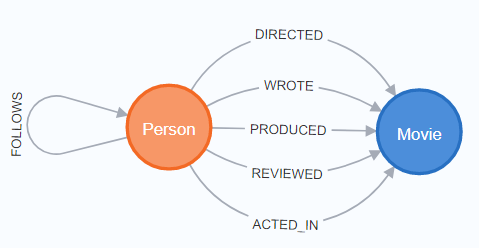
\includegraphics[width=0.75\linewidth,height=\textheight,keepaspectratio]{./images/img-095-072.png}

\begin{quote}
\textbf{GYAKORLAT:}

\begin{enumerate}
\def\labelenumi{\arabic{enumi}.}
\tightlist
\item
  Nyisd meg a Neo4j Desktop alkalmazást, és hozz létre egy új projektet.
\item
  Importáld a Movies mintaadatbázist (Add → Example Project).
\item
  Futtasd a \texttt{CALL\ db.schema.visualization()} parancsot, és
  tekintsd meg a sémát.
\item
  Próbáld ki a fenti Cypher-lekérdezéseket.
\end{enumerate}
\end{quote}

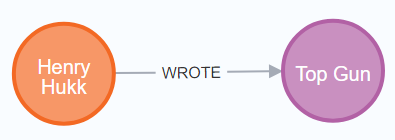
\includegraphics[width=0.75\linewidth,height=\textheight,keepaspectratio]{./images/img-096-073.png}

\begin{center}\rule{0.5\linewidth}{0.5pt}\end{center}

\subsection{Adatok importálása
Neo4j-be}\label{adatok-importuxe1luxe1sa-neo4j-be}

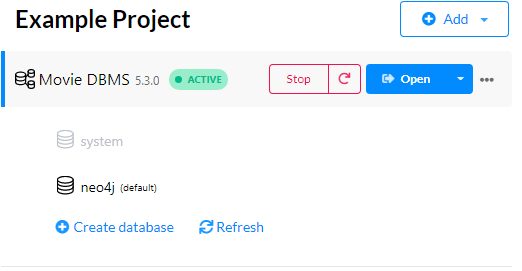
\includegraphics[width=0.75\linewidth,height=\textheight,keepaspectratio]{./images/img-097-074.png}

Az SQL Server adatai \textbf{CSV-fájlokon keresztül} importálhatók a
Neo4j-be. Első lépésként hozzuk létre a szükséges nézeteket a Northwind
adatbázisban:

\begin{Shaded}
\begin{Highlighting}[]
\KeywordTok{create} \KeywordTok{view}\NormalTok{ vi\_products }\KeywordTok{as}
\KeywordTok{select}\NormalTok{ ProductID, ProductName, CategoryID, UnitPrice, UnitsInStock}
\KeywordTok{from}\NormalTok{ Products;}

\KeywordTok{create} \KeywordTok{view}\NormalTok{ vi\_orders }\KeywordTok{as}
\KeywordTok{select}\NormalTok{ OrderID, CustomerID,}
   \FunctionTok{convert}\NormalTok{(}\DataTypeTok{varchar}\NormalTok{(}\DecValTok{10}\NormalTok{), OrderDate, }\DecValTok{120}\NormalTok{) }\KeywordTok{as}\NormalTok{ OrderDate, ShipCountry}
\KeywordTok{from}\NormalTok{ Orders;}

\KeywordTok{create} \KeywordTok{view}\NormalTok{ vi\_orders\_products }\KeywordTok{as}
\KeywordTok{select}\NormalTok{ od.OrderID, od.ProductID, od.Quantity, od.UnitPrice}
\KeywordTok{from}\NormalTok{ [}\KeywordTok{Order}\NormalTok{ Details] od;}
\end{Highlighting}
\end{Shaded}

Exportáld a nézeteket CSV-fájlokba, helyezd el a Neo4j \texttt{import/}
könyvtárában, majd Cypher \texttt{LOAD\ CSV} parancsokkal importáld:

\begin{Shaded}
\begin{Highlighting}[]
\NormalTok{// Termékek}
\NormalTok{LOAD CSV WITH HEADERS FROM \textquotesingle{}file:///vi\_products.csv\textquotesingle{} AS row}
\NormalTok{CREATE (:Product \{}
\NormalTok{ productId: toInteger(row.ProductID),}
\NormalTok{ name: row.ProductName,}
\NormalTok{ price: toFloat(row.UnitPrice),}
\NormalTok{ unitsInStock: toInteger(row.UnitsInStock)}
\NormalTok{\});}

\NormalTok{// Megrendelések}
\NormalTok{LOAD CSV WITH HEADERS FROM \textquotesingle{}file:///vi\_orders.csv\textquotesingle{} AS row}
\NormalTok{CREATE (:Order \{}
\NormalTok{ orderId: toInteger(row.OrderID),}
\NormalTok{ customerId: row.CustomerID,}
\NormalTok{ orderDate: row.OrderDate,}
\NormalTok{ shipCountry: row.ShipCountry}
\NormalTok{\});}

\NormalTok{// Kapcsolatok (rendelés–termék)}
\NormalTok{LOAD CSV WITH HEADERS FROM \textquotesingle{}file:///vi\_orders\_products.csv\textquotesingle{} AS row}
\NormalTok{MATCH (o:Order \{orderId: toInteger(row.OrderID)\})}
\NormalTok{MATCH (p:Product \{productId: toInteger(row.ProductID)\})}
\NormalTok{MERGE (o){-}[:CONTAINS \{quantity: toInteger(row.Quantity), unitPrice: toFloat(row.UnitPrice)\}]{-}\textgreater{}(p);}
\end{Highlighting}
\end{Shaded}

\begin{quote}
\textbf{GYAKORLAT:}

\begin{enumerate}
\def\labelenumi{\arabic{enumi}.}
\tightlist
\item
  Kérdezd le Cypher segítségével az éves bevételt terméknévenkénti
  bontásban, és hasonlítsd össze a relációs SQL-megoldással.
\item
  Generálj véletlenszerű gráfot T-SQL-lel az SQL Serverben, exportáld
  CSV-be, importáld Neo4j-be, és hasonlítsd meg a gráfátmérő mérésének
  futási idejét a két rendszerben.
\end{enumerate}
\end{quote}

\begin{center}\rule{0.5\linewidth}{0.5pt}\end{center}

\subsection{Képek és BLOB-ok
tárolása}\label{kuxe9pek-uxe9s-blob-ok-tuxe1roluxe1sa}

Az SQL Server két megközelítést kínál bináris nagy objektumok
(\textbf{BLOB} -- Binary Large Object) tárolásához.

\subsubsection{VARBINARY(MAX) --- közepes méretű
fájlokhoz}\label{varbinarymax-kuxf6zepes-muxe9retux171-fuxe1jlokhoz}

Az adatbázison belüli tárolás tranzakcióbiztos és egyszerűen
lekérdezhető. Néhány MB méretig ajánlott.

\begin{Shaded}
\begin{Highlighting}[]
\KeywordTok{create} \KeywordTok{table}\NormalTok{ my\_photos (}
 \KeywordTok{id} \DataTypeTok{integer}\NormalTok{ identity }\KeywordTok{primary} \KeywordTok{key}\NormalTok{,}
\NormalTok{ image\_name }\DataTypeTok{varchar}\NormalTok{(}\DecValTok{200}\NormalTok{),}
\NormalTok{ image\_column varbinary(}\FunctionTok{max}\NormalTok{)}
\NormalTok{);}

\CommentTok{{-}{-} Kép betöltése fájlból}
\KeywordTok{insert} \KeywordTok{into}\NormalTok{ my\_photos(image\_name, image\_column)}
\KeywordTok{select} \StringTok{\textquotesingle{}my\_photo.png\textquotesingle{}}\NormalTok{, }\OperatorTok{*} \KeywordTok{from}\NormalTok{ openrowset(}\KeywordTok{bulk} \StringTok{\textquotesingle{}c:\textbackslash{}my\_path\textbackslash{}my\_photo.png\textquotesingle{}}\NormalTok{, single\_blob) }\KeywordTok{as}\NormalTok{ img;}

\CommentTok{{-}{-} Fájlméretek lekérdezése}
\KeywordTok{select} \KeywordTok{id}\NormalTok{, image\_name, datalength(image\_column) }\KeywordTok{as}\NormalTok{ size\_bytes }\KeywordTok{from}\NormalTok{ my\_photos;}
\end{Highlighting}
\end{Shaded}

\subsubsection{FileTables --- nagy méretű
fájlokhoz}\label{filetables-nagy-muxe9retux171-fuxe1jlokhoz}

A \textbf{FileTable} az SQL Server \textbf{FILESTREAM} technológiájára
épül. A fájlok a fájlrendszeren tárolódnak, de SQL-táblakén is
elérhetők:

\begin{itemize}
\tightlist
\item
  Nagy méretű fájlokhoz (videó, hangfájl, dokumentum) ajánlott
\item
  Tranzakcióbiztos fájlkezelés
\item
  Windows fájlrendszer-API-val (UNC elérési út) és SQL-en keresztül
  egyaránt kezelhető
\item
  Előfeltétel: a SQL Server-példányon és az adatbázison engedélyezni
  kell a FILESTREAM-et
\end{itemize}

\begin{quote}
\textbf{GYAKORLAT:} tervezz FileTable-alapú megoldást a kurzus
képernyőfelvétel-videóinak tárolásához és lekérdezéséhez (cím, dátum és
időtartam szerint kereshetően).
\end{quote}

\begin{center}\rule{0.5\linewidth}{0.5pt}\end{center}

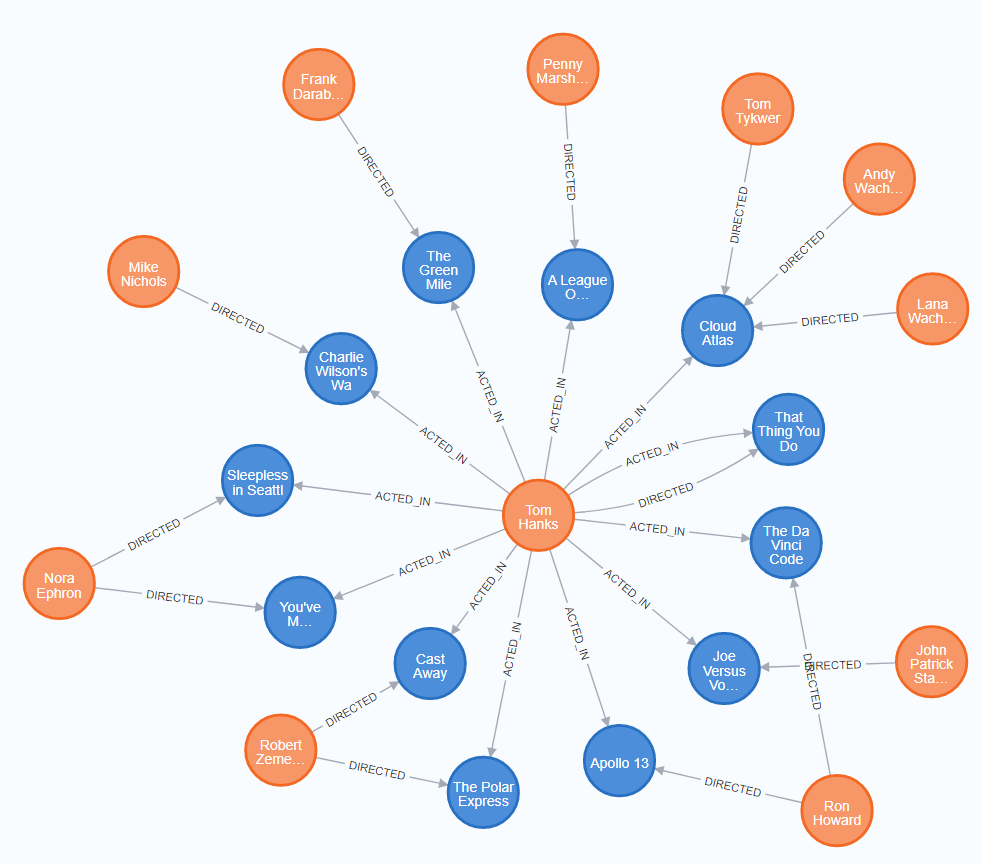
\includegraphics[width=0.75\linewidth,height=\textheight,keepaspectratio]{./images/img-098-075.png}

\section{9. Memóriaoptimalizált táblák az SQL
Serverben}\label{memuxf3riaoptimalizuxe1lt-tuxe1bluxe1k-az-sql-serverben}

A memóriaoptimalizált táblák (Memory-Optimized Tables, MOT) natívan
lefordított tárolt eljárásokkal kombinálva az OLTP relációs
adatbázis-technológia „Formula--1-je'',\footnote{https://learn.microsoft.com/en-us/sql/relational-databases/in-memory-oltp/overview-and-usage-scenarios?view=sql-server-ver16}
amelyet a memória árának csökkenése tett lehetővé.

\begin{center}\rule{0.5\linewidth}{0.5pt}\end{center}

\subsection{Jellemzők}\label{jellemzux151k}

\begin{itemize}
\tightlist
\item
  \textbf{Párhuzamos adatfeldolgozás}, finomított memóriabeli
  adatstruktúrák, hash indexek és önálló, dedikált memóriában működő
  adatbázismotor → nagy teljesítmény.

  \begin{itemize}
  \tightlist
  \item
    Minden MOT-táblaszerkezethez és natívan lefordított eljáráshoz egy
    új DLL jön létre.
  \item
    A zárolások elkerülése érdekében sorverziózást alkalmaz: egy sor
    frissítésekor a sor új verziója jön létre (= snapshot izoláció /
    pillanatkép-alapú izoláció). A törlések szintén logikai jellegűek: a
    törölt sorok mindaddig megőrződnek, amíg az adott verziót
    esetlegesen használó összes tranzakció véglegesítésre nem kerül.
  \end{itemize}
\item
  \textbf{Teljes ACID-támogatás.} A tartósságot a nem illékony
  (lemezalapú) tranzakciós napló biztosítja.
\item
  A MOT-ok \textbf{nem tartóssá (non-durable)} is tehetők, ha tranziens
  adatok tárolására használjuk őket --- a tempdb alternatívájaként. Az
  ilyen táblákban végzett módosítások nem igényelnek lemez I/O-t.
  További előny, hogy a táblák szerkezete --- ellentétben az ideiglenes
  táblákéval --- megmarad. A nem tartós MOT-ok gyorsítótárként
  (cache-ként) használhatók.
\item
  A MOT-ok hagyományos táblákkal \textbf{azonos adatbázisban} is
  elhelyezhetők.
\item
  Ha egy tárolt eljárás nincs natívan lefordítva, de MOT-ot használ,
  \textbf{értelmezett módban} kell futnia (a MOT-ot egy másik motor
  kezeli).\footnote{https://learn.microsoft.com/en-us/sql/relational-databases/in-memory-oltp/a-guide-to-query-processing-for-memory-optimized-tables}
\end{itemize}

\begin{center}\rule{0.5\linewidth}{0.5pt}\end{center}

\subsection[Követelmények és korlátozások]{\texorpdfstring{Követelmények
és
korlátozások\footnote{https://learn.microsoft.com/en-us/sql/relational-databases/in-memory-oltp/unsupported-sql-server-features-for-in-memory-oltp?view=sql-server-ver16}}{Követelmények és korlátozások}}\label{kuxf6vetelmuxe9nyek-uxe9s-korluxe1tozuxe1sok52}

\begin{itemize}
\item
  Csak \textbf{hash} vagy \textbf{nem fürtözött (nonclustered) BTree
  index} támogatott.
\item
  Elegendő memóriára van szükség:

  \begin{itemize}
  \tightlist
  \item
    a MOT és indexei számára,
  \item
    a sorverziózáshoz,
  \item
    táblaváltozókhoz és növekményes növekedéshez.
  \end{itemize}

  Ökölszabály: „a memóriaoptimalizált táblák és indexek várható
  méretének kétszeresével kezdj''.\footnote{https://learn.microsoft.com/en-us/sql/relational-databases/in-memory-oltp/estimate-memory-requirements-for-memory-optimized-tables?view=sql-server-ver16}
\item
  Egy MOT nem érhető el más adatbázisból (nincs adatbázisok közötti
  lekérdezés vagy tranzakció), és \textbf{nem particionálható}.
\item
  Az oldal- és sortömörítés, valamint a DDL-triggerek \textbf{nem
  támogatottak}.
\item
  MOT-előfizetővel csak \textbf{tranzakciós replikáció} támogatott.
\item
  DDL (CREATE / ALTER / DROP) tranzakciókon belül \textbf{nem
  támogatott}.
\item
  A natívan lefordított tárolt eljárások csak
  \textbf{memóriaoptimalizált táblákra} hivatkozhatnak.
\item
  \textbf{Identity} elsődleges kulcs szükséges.
\end{itemize}

\begin{center}\rule{0.5\linewidth}{0.5pt}\end{center}

\subsection{Ajánlott alkalmazási
területek}\label{ajuxe1nlott-alkalmazuxe1si-teruxfcletek}

\begin{itemize}
\tightlist
\item
  \textbf{Nagy teljesítményű tranzakció-feldolgozás}, pl. nagyszámú
  párhuzamos, alacsony késleltetésű tőzsdei tranzakció kezelése. A
  megvalósítás memóriaoptimalizált tranzakciós táblákat és natívan
  lefordított tárolt eljárásokat alkalmaz. Különösen a CPU-idő által
  dominált eljárások profitálnak a natív fordításból.
\item
  \textbf{Valós idejű adatgyűjtés és -transzformáció} sok forrásból (pl.
  IoT-érzékelők). Ha a tábla méretét korlátozni kell, egy ütemezett
  feladat segítségével az adatokat a memóriabeli táblából lemezalapú
  oszloptárba (column store) lehet áthelyezni. Ha sok frissítés van, az
  alaptábla egy temporális memóriaoptimalizált tábla lehet --- a korábbi
  rekordok lemezen maradnak.
\item
  \textbf{ETL-folyamat gyorsítása}: az adatraktár Extract-Transform-Load
  folyamatának staging tábláiként nem tartós, memóriaoptimalizált táblák
  használhatók. Ezek nem igényelnek lemez I/O-t, így felgyorsítják az
  ETL-folyamatot.
\item
  \textbf{Gyorsítótárazás (cache)}: egy nem tartós memóriabeli tábla
  kulcs-érték tárolóként (BLOB vagy JSON) is alkalmazható.
\item
  A \textbf{táblatípusok} szintén memóriaoptimalizálttá tehetők. Az
  ilyen típusok tárolt eljárások táblaértékű paramétereiként
  használhatók.
\end{itemize}

\begin{center}\rule{0.5\linewidth}{0.5pt}\end{center}

\subsection[GYAKORLAT --- Teljesítménymérés]{\texorpdfstring{GYAKORLAT
---
Teljesítménymérés\footnote{SQL Server 2022 nevű példányon a fájl
  memóriaoptimalizált filegroup-hoz való hozzáadása sikertelen a
  következő hibaüzenettel: \emph{„Could not process the operation.
  Always On Availability Groups replica manager is disabled on this
  instance\ldots{} etc.''} Ez ismert probléma. Helyette SQL Server 2019
  alapértelmezett példányát (nem nevezett példányt) használjuk.}}{GYAKORLAT --- Teljesítménymérés}}\label{gyakorlat-teljesuxedtmuxe9nymuxe9ruxe9s54}

Egy új tesztadatbázisban mérjük a MOT teljesítménybeli előnyét a normál
táblával szemben. Három forgatókönyvet hasonlítunk össze a
táblabeszúrások tekintetében:

\begin{enumerate}
\def\labelenumi{\arabic{enumi}.}
\tightlist
\item
  Lemezalapú tábla és értelmezett Transact-SQL
\item
  Memóriaoptimalizált tábla hash indexszel és értelmezett Transact-SQL
\item
  Memóriaoptimalizált tábla hash indexszel és natívan lefordított tárolt
  eljárás
\end{enumerate}

\begin{center}\rule{0.5\linewidth}{0.5pt}\end{center}

\subsection{Migráció tervezése In-Memory
megoldásra}\label{migruxe1ciuxf3-tervezuxe9se-in-memory-megolduxe1sra}

A migráció jelentős erőfeszítést igényelhet. Az SQL Server beépített
eszközöket kínál az OLTP → In-Memory átálláshoz.

\begin{quote}
\textbf{GYAKORLAT:}

\begin{itemize}
\tightlist
\item
  Töröld a Northwind adatbázist, és állítsd vissza a mentésből (dump).
\item
  Nyisd meg a \textbf{Database → Reports → Standard reports →
  Transaction Performance Analysis Overview} riportot. Az eszköz
  ajánlásokat ad a jelölt táblákhoz és eljárásokhoz. Kattints a
  tábla/eljárás nevére a részletes statisztikákhoz. A már
  memóriaoptimalizált táblák/eljárások nem szerepelnek a listában.
\item
  Az összesítő tábla létrehozásával ellenőrizheted a migrációs blokkolók
  (migration blockers) számát. A legrosszabb eset a Customers tábla 36
  blokkolóval --- ez a mentésfájl hibájára vezethető vissza (ugyanaz az
  idegen kulcs több példányban szerepel). Javítsd a mentésfájlt.
\item
  \textbf{Database → Tasks → Generate In-Memory OLTP Migration
  Checklists} (ez a funkció jelenleg nem működik).
\item
  Táblanév → \textbf{Table Memory Optimization Advisor}: első lépésként
  ellenőrzőlistát (checklist) generál. Az összes idegen kulcs
  megszorítást manuálisan kell eltávolítani a tábláról (és a táblára
  mutató megszorításokat is) az áttelepítés előtt, majd újra létre kell
  hozni.
\item
  Az Advisor megtervezi és végrehajtja az áttelepítést. A régi tábla
  megmarad, és átnevezésre kerül.
\end{itemize}
\end{quote}

\begin{center}\rule{0.5\linewidth}{0.5pt}\end{center}

\subsection{GYAKORLAT --- Reális forgatókönyv párhuzamos
munkamenetekkel}\label{gyakorlat-reuxe1lis-forgatuxf3kuxf6nyv-puxe1rhuzamos-munkamenetekkel}

Reálisabb forgatókönyvben a Northwind adatbázis rendelésfeldolgozó
tárolt eljárásának teljesítményét teszteljük párhuzamos munkamenetekben.

\begin{enumerate}
\def\labelenumi{\arabic{enumi}.}
\tightlist
\item
  Töröld az adatbázist, hozd létre újra a mentésből, és hozd létre az
  \texttt{sp\_new\_order()} eljárást.
\item
  Állítsd be a tesztelési paramétereket, majd futtasd az eljárást 10
  000-szer 3 párhuzamos munkamenetben Read Committed izolációval, és
  100-szor Repeatable Read izolációval. Mérd meg a futási időt.
\item
  Nézd át a \textbf{Transaction Performance Analysis Overview} riportot.
  A MOT-ra ajánlott táblák: Products, Orders, Order Details, Territories
  és Customers.
\item
  Telepítsd át a Products, Orders, Order Details és Customers táblákat:

  \begin{enumerate}
  \def\labelenumii{\alph{enumii}.}
  \tightlist
  \item
    Hozz létre egy új adatbázist \texttt{Northwind\_mot} névvel, és
    futtasd benne a javított dump szkriptet.
  \item
    Töröld az érintett táblákra mutató és az azoktól induló idegen kulcs
    megszorításokat.
  \item
    Telepítsd át a táblákat az Advisor segítségével. Ne felejdd
    belevenni az adatokat az új táblába.
  \end{enumerate}
\item
  Futtasd az alábbi parancsot:
\end{enumerate}

\begin{Shaded}
\begin{Highlighting}[]
\KeywordTok{alter} \KeywordTok{database} \KeywordTok{current} \KeywordTok{set}\NormalTok{ memory\_optimized\_elevate\_to\_snapshot }\OperatorTok{=} \KeywordTok{on}
\end{Highlighting}
\end{Shaded}

\begin{enumerate}
\def\labelenumi{\arabic{enumi}.}
\setcounter{enumi}{5}
\tightlist
\item
  Futtasd a régi rendelésfeldolgozó eljárást, teszteld, és hasonlítsd
  össze a futási időket.
\item
  Készítsd el a tárolt eljárás natívan lefordított változatát, és
  ismételd meg a teszteket.
\item
  Értelmezd az eredményeket!
\end{enumerate}

\begin{center}\rule{0.5\linewidth}{0.5pt}\end{center}

\section{10.
Köszönetnyilvánítás}\label{kuxf6szuxf6netnyilvuxe1nuxedtuxe1s}

Ezen kurzusjegyzet egyes példái Dejan Sarka, Matija Lah és Grega Jerkič
könyvén alapulnak: \emph{Exam 70-463: Implementing a Data Warehouse with
Microsoft SQL Server 2012}, Microsoft Press, ISBN 978-0-7356-6609-2,
2015. A többi hivatkozott példa forrása a lábjegyzetekben található.

\section{11. A függelék: SQL DML-példák önálló
tanuláshoz}\label{a-fuxfcggeluxe9k-sql-dml-puxe9lduxe1k-uxf6nuxe1lluxf3-tanuluxe1shoz}

Az alábbi példák a NORTHWIND adatbázison alapulnak. A lekérdezések egyre
összetettebbek; célszerű sorban haladni rajtuk.

\begin{center}\rule{0.5\linewidth}{0.5pt}\end{center}

\subsection{Alapvető SELECT
lekérdezések}\label{alapvetux151-select-lekuxe9rdezuxe9sek}

\begin{Shaded}
\begin{Highlighting}[]
\KeywordTok{use}\NormalTok{ NORTHWIND}
\KeywordTok{select} \OperatorTok{*} \KeywordTok{from}\NormalTok{ employees}
\KeywordTok{select}\NormalTok{ lastname, birthdate }\KeywordTok{from}\NormalTok{ employees}

\CommentTok{{-}{-}a Londonban található ügyfelek neve}
\KeywordTok{select}\NormalTok{ companyname, city}
\KeywordTok{from}\NormalTok{ customers}
\CommentTok{{-}{-}where city LIKE \textquotesingle{}L\%\textquotesingle{} and (city LIKE \textquotesingle{}\%b\%\textquotesingle{} or city LIKE \textquotesingle{}\%n\%\textquotesingle{}) {-}{-}részleges egyezés}
\KeywordTok{where}\NormalTok{ city }\KeywordTok{IN}\NormalTok{ (}\StringTok{\textquotesingle{}London\textquotesingle{}}\NormalTok{, }\StringTok{\textquotesingle{}Lander\textquotesingle{}}\NormalTok{)}
\KeywordTok{where}\NormalTok{ city }\OperatorTok{=}\StringTok{\textquotesingle{}London\textquotesingle{}} \KeywordTok{or}\NormalTok{ city }\OperatorTok{=}\StringTok{\textquotesingle{}Lander\textquotesingle{}}
\KeywordTok{where}\NormalTok{ city }\KeywordTok{IN}\NormalTok{ (}\StringTok{\textquotesingle{}London\textquotesingle{}}\NormalTok{)}
\KeywordTok{where}\NormalTok{ city }\OperatorTok{=} \StringTok{\textquotesingle{}London\textquotesingle{}}
\end{Highlighting}
\end{Shaded}

\begin{center}\rule{0.5\linewidth}{0.5pt}\end{center}

\subsection{Aggregáló függvények és beágyazott
lekérdezések}\label{aggreguxe1luxf3-fuxfcggvuxe9nyek-uxe9s-beuxe1gyazott-lekuxe9rdezuxe9sek}

\begin{Shaded}
\begin{Highlighting}[]
\CommentTok{{-}{-}Ki a legfiatalabb alkalmazott? Mi a neve?}
\CommentTok{{-}{-}1/2) a legnagyobb születési dátum}
\CommentTok{{-}{-}aggregáló függvények: max, min, avg, std, sum, count}
\KeywordTok{select} \FunctionTok{max}\NormalTok{(birthdate) }\KeywordTok{as}\NormalTok{ max\_year, }\FunctionTok{min}\NormalTok{(birthdate) }\KeywordTok{as}\NormalTok{ min\_year}
\CommentTok{{-}{-}, lastname {-}{-}hibát okozna}
\KeywordTok{from}\NormalTok{ employees}

\CommentTok{{-}{-}2/2) ágyazd be ezt a lekérdezést}
\KeywordTok{select}\NormalTok{ lastname, birthdate }\KeywordTok{from}\NormalTok{ employees}
\KeywordTok{where}\NormalTok{ birthdate }\OperatorTok{=}\NormalTok{ (}\StringTok{\textquotesingle{}1966{-}01{-}27 00:00:00.000\textquotesingle{}}\NormalTok{)}

\KeywordTok{select}\NormalTok{ lastname, birthdate }\KeywordTok{as} \OtherTok{"birth date"} \KeywordTok{from}\NormalTok{ employees}
\KeywordTok{where}\NormalTok{ birthdate }\OperatorTok{=}\NormalTok{ (}
  \KeywordTok{select} \FunctionTok{max}\NormalTok{(birthdate) }\KeywordTok{as}\NormalTok{ max\_year}
  \KeywordTok{from}\NormalTok{ employees}
\NormalTok{)}

\CommentTok{{-}{-}FELADAT: keresd meg az első rendelés ShipAddress mezőjét}
\KeywordTok{select}\NormalTok{ orderdate, shipaddress }\KeywordTok{from}\NormalTok{ orders}
\KeywordTok{where}\NormalTok{ orderdate }\OperatorTok{=}\NormalTok{ (}
  \KeywordTok{select} \FunctionTok{min}\NormalTok{(orderdate) }\KeywordTok{as}\NormalTok{ min\_date}
  \KeywordTok{from}\NormalTok{ orders}
\NormalTok{)}

\CommentTok{{-}{-}a legfiatalabb alkalmazott szállítási címei}
\CommentTok{{-}{-}táblák összekapcsolása}
\KeywordTok{select} \KeywordTok{distinct}\NormalTok{ lastname, shipaddress}
\KeywordTok{from}\NormalTok{ orders o }\KeywordTok{inner} \KeywordTok{join}\NormalTok{ employees e }\KeywordTok{on}\NormalTok{ o.employeeid}\OperatorTok{=}\NormalTok{e.employeeid}
\KeywordTok{where}\NormalTok{ e.employeeid }\OperatorTok{=}\NormalTok{ (}
  \KeywordTok{select}\NormalTok{ employeeid }\KeywordTok{from}\NormalTok{ employees}
  \KeywordTok{where}\NormalTok{ birthdate }\OperatorTok{=}\NormalTok{ (}
    \KeywordTok{select} \FunctionTok{max}\NormalTok{(birthdate) }\KeywordTok{as}\NormalTok{ max\_year}
    \KeywordTok{from}\NormalTok{ employees}
\NormalTok{  )}
\NormalTok{)}
\KeywordTok{order} \KeywordTok{by}\NormalTok{ shipaddress }\CommentTok{{-}{-}desc}
\end{Highlighting}
\end{Shaded}

\begin{center}\rule{0.5\linewidth}{0.5pt}\end{center}

\subsection{JOIN-ok}\label{join-ok}

\begin{Shaded}
\begin{Highlighting}[]
\CommentTok{{-}{-}milyen termékeket rendeltek a legfiatalabb alkalmazottól}
\CommentTok{{-}{-}megjegyzés: mindig a lekérdezés FROM részével kezdjünk}
\KeywordTok{select} \KeywordTok{distinct}\NormalTok{ p.productname, e.lastname}
\KeywordTok{from}\NormalTok{ orders o }\KeywordTok{inner} \KeywordTok{join}\NormalTok{ employees e }\KeywordTok{on}\NormalTok{ o.employeeid}\OperatorTok{=}\NormalTok{e.employeeid}
\KeywordTok{inner} \KeywordTok{join}\NormalTok{ [}\KeywordTok{order}\NormalTok{ details] od }\KeywordTok{on}\NormalTok{ od.orderid}\OperatorTok{=}\NormalTok{o.orderid}
\KeywordTok{inner} \KeywordTok{join}\NormalTok{ products p }\KeywordTok{on}\NormalTok{ p.productid}\OperatorTok{=}\NormalTok{od.productid}
\KeywordTok{where}\NormalTok{ e.employeeid}\OperatorTok{=}\DecValTok{9} \CommentTok{{-}{-}ő a legfiatalabb}
\KeywordTok{order} \KeywordTok{by}\NormalTok{ productname}

\CommentTok{{-}{-}FELADAT: mely városokba szállítják az 1{-}es kategóriájú termékeket?}
\KeywordTok{select} \KeywordTok{distinct}\NormalTok{ o.shipcity}
\KeywordTok{from}\NormalTok{ orders o }\KeywordTok{inner} \KeywordTok{join}\NormalTok{ [}\KeywordTok{order}\NormalTok{ details] od }\KeywordTok{on}\NormalTok{ od.orderid}\OperatorTok{=}\NormalTok{o.orderid}
\KeywordTok{inner} \KeywordTok{join}\NormalTok{ products p }\KeywordTok{on}\NormalTok{ p.productid}\OperatorTok{=}\NormalTok{od.productid}
\KeywordTok{where}\NormalTok{ p.categoryid }\OperatorTok{=} \DecValTok{1} \CommentTok{{-}{-}a keresési feltételünk}
\KeywordTok{order} \KeywordTok{by}\NormalTok{ shipcity}
\end{Highlighting}
\end{Shaded}

\begin{center}\rule{0.5\linewidth}{0.5pt}\end{center}

\subsection{Csoportosítás (GROUP
BY)}\label{csoportosuxedtuxe1s-group-by}

Az alábbi sorozat bemutatja, hogyan érdemes felépíteni egy összetett
GROUP BY lekérdezést. A számok a helyes írási sorrendet jelzik (FROM →
GROUP BY → SELECT → ORDER BY).

\begin{Shaded}
\begin{Highlighting}[]
\CommentTok{{-}{-}Hány rendelése van alkalmazottanként?}
\CommentTok{{-}{-}1/5) CSOPORTOSÍTÁS}
\KeywordTok{select}\NormalTok{ employeeid, }\FunctionTok{count}\NormalTok{(}\OperatorTok{*}\NormalTok{)}
\KeywordTok{from}\NormalTok{ orders}
\KeywordTok{group} \KeywordTok{by}\NormalTok{ employeeid}

\CommentTok{{-}{-}mellékes megjegyzés: hogyan teszteljük a NULL értéket?}
\KeywordTok{select} \OperatorTok{*} \KeywordTok{from}\NormalTok{ orders }\KeywordTok{where}\NormalTok{ employeeid }\KeywordTok{is} \KeywordTok{null}
\KeywordTok{delete} \KeywordTok{from}\NormalTok{ orders }\KeywordTok{where}\NormalTok{ employeeid }\KeywordTok{is} \KeywordTok{null}

\CommentTok{{-}{-}2/5) NE CSINÁLD EZT:}
\KeywordTok{select}\NormalTok{ e.lastname, }\FunctionTok{count}\NormalTok{(}\OperatorTok{*}\NormalTok{)}
\KeywordTok{from}\NormalTok{ orders o }\KeywordTok{inner} \KeywordTok{join}\NormalTok{ employees e }\KeywordTok{on}\NormalTok{ o.employeeid}\OperatorTok{=}\NormalTok{e.employeeid}
\KeywordTok{group} \KeywordTok{by}\NormalTok{ e.lastname}
\CommentTok{{-}{-}logikai hibát okoz, ha két személynek azonos a vezetékneve!!!}

\CommentTok{{-}{-}3/5)}
\KeywordTok{select}\NormalTok{ e.lastname, e.firstname, }\FunctionTok{count}\NormalTok{(}\OperatorTok{*}\NormalTok{)}
\KeywordTok{from}\NormalTok{ orders o }\KeywordTok{inner} \KeywordTok{join}\NormalTok{ employees e }\KeywordTok{on}\NormalTok{ o.employeeid}\OperatorTok{=}\NormalTok{e.employeeid}
\KeywordTok{group} \KeywordTok{by}\NormalTok{ e.employeeid, e.lastname, e.firstname}
\CommentTok{{-}{-}ez a lekérdezés kihagyja azt az alkalmazottat, akinek nincs rendelése}

\CommentTok{{-}{-}FELADAT: listázd ki az egyes kategóriákban lévő termékek számát (a CategoryName{-}re is szükségünk van)}
\FloatTok{3.} \KeywordTok{select}\NormalTok{ c.categoryid, c.categoryname, }\FunctionTok{count}\NormalTok{(}\OperatorTok{*}\NormalTok{) }\KeywordTok{as}\NormalTok{ no\_prod}
\FloatTok{1.} \KeywordTok{from}\NormalTok{ products p }\KeywordTok{inner} \KeywordTok{join}\NormalTok{ categories c }\KeywordTok{on}\NormalTok{ p.categoryid}\OperatorTok{=}\NormalTok{c.categoryid}
\FloatTok{2.} \KeywordTok{group} \KeywordTok{by}\NormalTok{ c.categoryid, c.categoryname}
\FloatTok{4.} \KeywordTok{order} \KeywordTok{by}\NormalTok{ no\_prod }\KeywordTok{desc}

\CommentTok{{-}{-}4/5)}
\KeywordTok{select}\NormalTok{ e.employeeid, e.lastname, e.firstname, }\FunctionTok{count}\NormalTok{(}\OperatorTok{*}\NormalTok{)}
\KeywordTok{from}\NormalTok{ employees e }\KeywordTok{left} \KeywordTok{outer} \KeywordTok{join}\NormalTok{ orders o }\KeywordTok{on}\NormalTok{ o.employeeid}\OperatorTok{=}\NormalTok{e.employeeid}
\KeywordTok{group} \KeywordTok{by}\NormalTok{ e.employeeid, e.lastname, e.firstname}
\CommentTok{{-}{-}probléma: a tétlen alkalmazott hamisan 1{-}es darabszámot kap}

\CommentTok{{-}{-}5/5)}
\KeywordTok{select}\NormalTok{ e.employeeid, e.lastname, e.firstname, }\FunctionTok{count}\NormalTok{(o.orderid) }\KeywordTok{as}\NormalTok{ no\_ord}
\KeywordTok{from}\NormalTok{ employees e }\KeywordTok{left} \KeywordTok{outer} \KeywordTok{join}\NormalTok{ orders o }\KeywordTok{on}\NormalTok{ o.employeeid}\OperatorTok{=}\NormalTok{e.employeeid}
\KeywordTok{group} \KeywordTok{by}\NormalTok{ e.employeeid, e.lastname, e.firstname}
\KeywordTok{order} \KeywordTok{by}\NormalTok{ no\_ord }\KeywordTok{desc}
\CommentTok{{-}{-}minden probléma megoldva}
\end{Highlighting}
\end{Shaded}

\begin{center}\rule{0.5\linewidth}{0.5pt}\end{center}

\subsection{Önillesztés (hierarchia
lekérdezése)}\label{uxf6nillesztuxe9s-hierarchia-lekuxe9rdezuxe9se}

\begin{Shaded}
\begin{Highlighting}[]
\CommentTok{{-}{-}ki kinek a főnöke}
\KeywordTok{select}\NormalTok{ e.lastname, boss.lastname }\KeywordTok{as}\NormalTok{ boss, bboss.lastname }\KeywordTok{as}\NormalTok{ boss\_of\_boss}
\KeywordTok{from}\NormalTok{ employees e }\KeywordTok{left} \KeywordTok{outer} \KeywordTok{join}\NormalTok{ employees boss }\KeywordTok{on}\NormalTok{ e.reportsto}\OperatorTok{=}\NormalTok{boss.employeeid}
\KeywordTok{left} \KeywordTok{outer} \KeywordTok{join}\NormalTok{ employees bboss }\KeywordTok{on}\NormalTok{ boss.reportsto}\OperatorTok{=}\NormalTok{bboss.employeeid}

\CommentTok{{-}{-}Hány rendelése van alkalmazottanként?}
\KeywordTok{select}\NormalTok{ e.lastname, }\FunctionTok{count}\NormalTok{(orderid)}
\CommentTok{{-}{-}a count(*) hamisan egy rendelést adna Lamernek, akinek valójában nincs rendelése}
\KeywordTok{from}\NormalTok{ employees e }\KeywordTok{left} \KeywordTok{outer} \KeywordTok{join}\NormalTok{ orders o }\KeywordTok{on}
\CommentTok{{-}{-}from employees e inner join orders o on}
\NormalTok{e.employeeid }\OperatorTok{=}\NormalTok{ o.employeeid}
\KeywordTok{group} \KeywordTok{by}\NormalTok{ e.employeeid, e.lastname}
\KeywordTok{order} \KeywordTok{by} \FunctionTok{count}\NormalTok{(}\OperatorTok{*}\NormalTok{) }\KeywordTok{desc}

\CommentTok{{-}{-}kinek nincs rendelése?}
\KeywordTok{select}\NormalTok{ e.}\OperatorTok{*}
\KeywordTok{from}\NormalTok{ employees e }\KeywordTok{left} \KeywordTok{outer} \KeywordTok{join}\NormalTok{ orders o }\KeywordTok{on}
\NormalTok{e.employeeid }\OperatorTok{=}\NormalTok{ o.employeeid}
\KeywordTok{where}\NormalTok{ o.orderid }\KeywordTok{is} \KeywordTok{null}
\end{Highlighting}
\end{Shaded}

\begin{center}\rule{0.5\linewidth}{0.5pt}\end{center}

\subsection{Aritmetika, STR()
formázás}\label{aritmetika-str-formuxe1zuxe1s}

\begin{Shaded}
\begin{Highlighting}[]
\CommentTok{{-}{-}melyik a legnagyobb rendelés?}
\CommentTok{{-}{-}aritmetika}
\FloatTok{4.} \KeywordTok{select}\NormalTok{ o.orderid,}
 \FunctionTok{cast}\NormalTok{(o.orderdate }\KeywordTok{as} \DataTypeTok{varchar}\NormalTok{(}\DecValTok{50}\NormalTok{)) }\KeywordTok{as}\NormalTok{ order\_date,}
\NormalTok{ str(}\FunctionTok{sum}\NormalTok{((}\DecValTok{1}\OperatorTok{{-}}\NormalTok{discount)}\OperatorTok{*}\NormalTok{unitprice}\OperatorTok{*}\NormalTok{quantity), }\DecValTok{15}\NormalTok{, }\DecValTok{2}\NormalTok{) }\KeywordTok{as}\NormalTok{ order\_total,}
 \FunctionTok{sum}\NormalTok{(quantity) }\KeywordTok{as}\NormalTok{ no\_of\_units,}
 \FunctionTok{count}\NormalTok{(d.orderid) }\KeywordTok{as}\NormalTok{ no\_of\_items}
\FloatTok{1.} \KeywordTok{from}\NormalTok{ orders o }\KeywordTok{inner} \KeywordTok{join}\NormalTok{ [}\KeywordTok{order}\NormalTok{ details] d }\KeywordTok{on}\NormalTok{ o.orderid}\OperatorTok{=}\NormalTok{d.orderid}
\FloatTok{2.} \KeywordTok{where}\OperatorTok{..}\NormalTok{.}
\FloatTok{3.} \KeywordTok{group} \KeywordTok{by}\NormalTok{ o.orderid, o.orderdate}
 \CommentTok{{-}{-}order by o.orderdate}
\FloatTok{5.} \KeywordTok{order} \KeywordTok{by} \FunctionTok{sum}\NormalTok{((}\DecValTok{1}\OperatorTok{{-}}\NormalTok{discount)}\OperatorTok{*}\NormalTok{unitprice}\OperatorTok{*}\NormalTok{quantity) }\KeywordTok{desc}
\end{Highlighting}
\end{Shaded}

\begin{center}\rule{0.5\linewidth}{0.5pt}\end{center}

\subsection{HAVING, ISNULL, a legjobb
értékesítő}\label{having-isnull-a-legjobb-uxe9rtuxe9kesuxedtux151}

\begin{Shaded}
\begin{Highlighting}[]
\CommentTok{{-}{-}ki a legsikeresebb alkalmazott? hány rendeléssel?}
\CommentTok{{-}{-} figyeld meg: having}
\CommentTok{{-}{-} count distinct}
\CommentTok{{-}{-} számok formázása}
\KeywordTok{select}\NormalTok{ u.titleofcourtesy}\OperatorTok{+}\StringTok{\textquotesingle{} \textquotesingle{}}\OperatorTok{+}\NormalTok{u.lastname}\OperatorTok{+}\StringTok{\textquotesingle{} \textquotesingle{}}\OperatorTok{+}\NormalTok{ u.firstname }\OperatorTok{+}\StringTok{\textquotesingle{} (\textquotesingle{}}\OperatorTok{+}\NormalTok{u.title }\OperatorTok{+}\StringTok{\textquotesingle{})\textquotesingle{}} \KeywordTok{as}\NormalTok{ name,}
\NormalTok{str(}\FunctionTok{sum}\NormalTok{((}\DecValTok{1}\OperatorTok{{-}}\NormalTok{discount)}\OperatorTok{*}\NormalTok{unitprice}\OperatorTok{*}\NormalTok{quantity), }\DecValTok{15}\NormalTok{, }\DecValTok{2}\NormalTok{) }\KeywordTok{as}\NormalTok{ cash\_income,}
\FunctionTok{count}\NormalTok{(}\KeywordTok{distinct}\NormalTok{ o.orderid) }\KeywordTok{as}\NormalTok{ no\_of\_orders, }\FunctionTok{count}\NormalTok{(productid) }\KeywordTok{as}\NormalTok{ no\_of\_items}
\KeywordTok{from}\NormalTok{ orders o }\KeywordTok{inner} \KeywordTok{join}\NormalTok{ [}\KeywordTok{order}\NormalTok{ details] d }\KeywordTok{on}\NormalTok{ o.orderid}\OperatorTok{=}\NormalTok{d.orderid}
\KeywordTok{inner} \KeywordTok{join}\NormalTok{ employees u }\KeywordTok{on}\NormalTok{ u.employeeid}\OperatorTok{=}\NormalTok{o.employeeid}
\KeywordTok{group} \KeywordTok{by}\NormalTok{ u.employeeid, u.titleofcourtesy, u.title, u.lastname, u.firstname}
\CommentTok{{-}{-}having count(o.orderid)\textgreater{}200 {-}{-}ha csak a több mint 200 rendeléssel rendelkező alkalmazottak érdekelnek}
\KeywordTok{order} \KeywordTok{by}\NormalTok{ cash\_income}
\CommentTok{{-}{-}sum((1{-}discount)*unitprice*quantity) desc}

\CommentTok{{-}{-}miért csak 9 van?}
\KeywordTok{select} \FunctionTok{count}\NormalTok{(}\OperatorTok{*}\NormalTok{) }\KeywordTok{from}\NormalTok{ employees}
\CommentTok{{-}{-}10{-}nek kellene lennie!}
\CommentTok{{-}{-}szükségünk lenne azokra is, akiknek 0 rendelésük van}
\CommentTok{{-}{-} isnull függvény}
\KeywordTok{select}\NormalTok{ isnull(u.titleofcourtesy, }\StringTok{\textquotesingle{}\textquotesingle{}}\NormalTok{)}\OperatorTok{+}\StringTok{\textquotesingle{} \textquotesingle{}}\OperatorTok{+}\NormalTok{isnull(u.lastname, }\StringTok{\textquotesingle{}\textquotesingle{}}\NormalTok{)}\OperatorTok{+}\StringTok{\textquotesingle{} \textquotesingle{}}\OperatorTok{+}\NormalTok{ isnull(u.firstname,}
\StringTok{\textquotesingle{}\textquotesingle{}}\NormalTok{) }\OperatorTok{+}\StringTok{\textquotesingle{} (\textquotesingle{}}\OperatorTok{+}\NormalTok{isnull(u.title, }\StringTok{\textquotesingle{}\textquotesingle{}}\NormalTok{) }\OperatorTok{+}\StringTok{\textquotesingle{})\textquotesingle{}} \KeywordTok{as}\NormalTok{ name,}
\NormalTok{isnull(str(}\FunctionTok{sum}\NormalTok{((}\DecValTok{1}\OperatorTok{{-}}\NormalTok{discount)}\OperatorTok{*}\NormalTok{unitprice}\OperatorTok{*}\NormalTok{quantity), }\DecValTok{15}\NormalTok{, }\DecValTok{2}\NormalTok{), }\StringTok{\textquotesingle{}N/A\textquotesingle{}}\NormalTok{) }\KeywordTok{as}\NormalTok{ cash\_income,}
\FunctionTok{count}\NormalTok{(}\KeywordTok{distinct}\NormalTok{ o.orderid) }\KeywordTok{as}\NormalTok{ no\_of\_orders, }\FunctionTok{COUNT}\NormalTok{(d.productid) }\KeywordTok{as}\NormalTok{ no\_of\_items}
\KeywordTok{from}\NormalTok{ employees u }\KeywordTok{left} \KeywordTok{outer} \KeywordTok{join}
\NormalTok{(orders o }\KeywordTok{inner} \KeywordTok{join}\NormalTok{ [}\KeywordTok{order}\NormalTok{ details] d }\KeywordTok{on}\NormalTok{ o.orderid}\OperatorTok{=}\NormalTok{d.orderid)}
\KeywordTok{on}\NormalTok{ u.employeeid}\OperatorTok{=}\NormalTok{o.employeeid}
\CommentTok{{-}{-}where u.titleofcourtesy=\textquotesingle{}Mr.\textquotesingle{} {-}{-}ha csak a férfiak érdekelnek}
\KeywordTok{group} \KeywordTok{by}\NormalTok{ u.employeeid, u.titleofcourtesy, u.title, u.lastname, u.firstname}
\KeywordTok{order} \KeywordTok{by} \FunctionTok{sum}\NormalTok{((}\DecValTok{1}\OperatorTok{{-}}\NormalTok{discount)}\OperatorTok{*}\NormalTok{unitprice}\OperatorTok{*}\NormalTok{quantity) }\KeywordTok{desc}
\end{Highlighting}
\end{Shaded}

\begin{center}\rule{0.5\linewidth}{0.5pt}\end{center}

\subsection{TOP --- a legnépszerűbb
termék}\label{top-a-legnuxe9pszerux171bb-termuxe9k}

\begin{Shaded}
\begin{Highlighting}[]
\CommentTok{{-}{-}melyik a legnépszerűbb termék?}
\CommentTok{{-}{-} top 1}
\KeywordTok{select}\NormalTok{ top }\DecValTok{1}\NormalTok{ p.productid, p.productname, }\FunctionTok{count}\NormalTok{(}\OperatorTok{*}\NormalTok{) }\KeywordTok{as}\NormalTok{ no\_app,}
\FunctionTok{sum}\NormalTok{(quantity) }\KeywordTok{as}\NormalTok{ total\_pieces}
\KeywordTok{from}\NormalTok{ products p }\KeywordTok{left} \KeywordTok{outer} \KeywordTok{join}\NormalTok{ [}\KeywordTok{order}\NormalTok{ details] d }\KeywordTok{on}\NormalTok{ p.productid}\OperatorTok{=}\NormalTok{d.productid}
\KeywordTok{group} \KeywordTok{by}\NormalTok{ p.productid, p.productname}
\KeywordTok{order} \KeywordTok{by}\NormalTok{ no\_app }\KeywordTok{desc}

\CommentTok{{-}{-}melyik alkalmazott adta el a legtöbbet a legnépszerűbb termékből?}
\CommentTok{{-}{-}első verzió}
\KeywordTok{select}\NormalTok{ top }\DecValTok{1}\NormalTok{ u.titleofcourtesy}\OperatorTok{+}\StringTok{\textquotesingle{} \textquotesingle{}}\OperatorTok{+}\NormalTok{u.lastname}\OperatorTok{+}\StringTok{\textquotesingle{} \textquotesingle{}}\OperatorTok{+}\NormalTok{ u.firstname }\OperatorTok{+}\StringTok{\textquotesingle{} (\textquotesingle{}}\OperatorTok{+}\NormalTok{u.title }\OperatorTok{+}\StringTok{\textquotesingle{})\textquotesingle{}} \KeywordTok{as}\NormalTok{ name,}
\FunctionTok{sum}\NormalTok{(quantity) }\KeywordTok{as}\NormalTok{ no\_pieces\_sold}
\KeywordTok{from}\NormalTok{ orders o }\KeywordTok{inner} \KeywordTok{join}\NormalTok{ [}\KeywordTok{order}\NormalTok{ details] d }\KeywordTok{on}\NormalTok{ o.orderid}\OperatorTok{=}\NormalTok{d.orderid}
\KeywordTok{inner} \KeywordTok{join}\NormalTok{ employees u }\KeywordTok{on}\NormalTok{ u.employeeid}\OperatorTok{=}\NormalTok{o.employeeid}
\KeywordTok{where}\NormalTok{ d.productid }\OperatorTok{=} \DecValTok{59} \CommentTok{{-}{-}ezt már tudjuk}
\KeywordTok{group} \KeywordTok{by}\NormalTok{ u.employeeid, u.titleofcourtesy, u.title, u.lastname, u.firstname}
\CommentTok{{-}{-} having....}
\KeywordTok{order} \KeywordTok{by} \FunctionTok{sum}\NormalTok{(quantity) }\KeywordTok{desc}

\CommentTok{/************************************************************************}
\CommentTok{FELADAT}
\CommentTok{{-}{-}melyik alkalmazott adta el a legtöbbet a legnépszerűbb termékből, és mi annak a}
\CommentTok{terméknek a neve?}
\CommentTok{{-}{-}a pubs\_access adatbázisban: melyik a leggyakrabban használt kiadó annál a szerzőnél, akinek}
\CommentTok{a legtöbb publikációja van?}
\CommentTok{**************************************************************************/}
\end{Highlighting}
\end{Shaded}

\begin{center}\rule{0.5\linewidth}{0.5pt}\end{center}

\subsection{Dátumfüggvények}\label{duxe1tumfuxfcggvuxe9nyek}

\begin{Shaded}
\begin{Highlighting}[]
\CommentTok{{-}{-}TÖBBSZINTŰ CSOPORTOSÍTÁS}
\CommentTok{{-}{-}dátum{-} és időfüggvények}
\KeywordTok{select} \DecValTok{2}
\KeywordTok{select}\NormalTok{ getdate() }\CommentTok{{-}{-}datetime adattípus}
\KeywordTok{select}\NormalTok{ DATEDIFF(s,}\StringTok{\textquotesingle{}2013{-}10{-}10 12:13:50.370\textquotesingle{}}\NormalTok{, }\StringTok{\textquotesingle{}2013{-}10{-}10 14:16:50.370\textquotesingle{}}\NormalTok{)}
\KeywordTok{select}\NormalTok{ DATEADD(s, }\DecValTok{1000}\NormalTok{, }\StringTok{\textquotesingle{}2013{-}10{-}10 14:16:50.370\textquotesingle{}}\NormalTok{)}
\KeywordTok{select} \DataTypeTok{YEAR}\NormalTok{(getdate()), }\DataTypeTok{MONTH}\NormalTok{(getdate())}

\CommentTok{{-}{-}RENDELÉSEK HÓNAP ÉS ALKALMAZOTT SZERINT}
\KeywordTok{select}\NormalTok{ e.employeeid, lastname, }\DataTypeTok{year}\NormalTok{(orderdate) }\KeywordTok{as} \DataTypeTok{year}\NormalTok{, }\DataTypeTok{month}\NormalTok{(orderdate) }\KeywordTok{as} \DataTypeTok{month}\NormalTok{,}
\FunctionTok{count}\NormalTok{(orderid) }\KeywordTok{as}\NormalTok{ no\_of\_orders}
\KeywordTok{from}\NormalTok{ employees e }\KeywordTok{left} \KeywordTok{outer} \KeywordTok{join}\NormalTok{ orders o }\KeywordTok{on}\NormalTok{ e.employeeid}\OperatorTok{=}\NormalTok{o.employeeid}
\KeywordTok{group} \KeywordTok{by}\NormalTok{ e.employeeid, lastname, }\DataTypeTok{year}\NormalTok{(orderdate), }\DataTypeTok{month}\NormalTok{(orderdate)}
\KeywordTok{order} \KeywordTok{by}\NormalTok{ lastname, }\DataTypeTok{year}\NormalTok{, }\DataTypeTok{month}

\CommentTok{{-}{-}ugyanez másképpen:}
\KeywordTok{select}\NormalTok{ e.employeeid, lastname,}
\FunctionTok{cast}\NormalTok{(}\DataTypeTok{year}\NormalTok{(orderdate) }\KeywordTok{as} \DataTypeTok{varchar}\NormalTok{(}\DecValTok{4}\NormalTok{)) }\OperatorTok{+}\StringTok{\textquotesingle{}\_\textquotesingle{}}\OperatorTok{+} \FunctionTok{cast}\NormalTok{(}\DataTypeTok{month}\NormalTok{(orderdate) }\KeywordTok{as} \DataTypeTok{char}\NormalTok{(}\DecValTok{2}\NormalTok{)) }\KeywordTok{as} \DataTypeTok{month}\NormalTok{,}
\FunctionTok{count}\NormalTok{(orderid) }\KeywordTok{as}\NormalTok{ no\_of\_orders}
\KeywordTok{from}\NormalTok{ employees e }\KeywordTok{left} \KeywordTok{outer} \KeywordTok{join}\NormalTok{ orders o }\KeywordTok{on}\NormalTok{ e.employeeid}\OperatorTok{=}\NormalTok{o.employeeid}
\KeywordTok{group} \KeywordTok{by}\NormalTok{ e.employeeid, lastname, }\FunctionTok{cast}\NormalTok{(}\DataTypeTok{year}\NormalTok{(orderdate) }\KeywordTok{as} \DataTypeTok{varchar}\NormalTok{(}\DecValTok{4}\NormalTok{)) }\OperatorTok{+}\StringTok{\textquotesingle{}\_\textquotesingle{}}\OperatorTok{+}
\FunctionTok{cast}\NormalTok{(}\DataTypeTok{month}\NormalTok{(orderdate) }\KeywordTok{as} \DataTypeTok{char}\NormalTok{(}\DecValTok{2}\NormalTok{))}
\KeywordTok{order} \KeywordTok{by}\NormalTok{ lastname, }\DataTypeTok{month}
\end{Highlighting}
\end{Shaded}

\begin{center}\rule{0.5\linewidth}{0.5pt}\end{center}

\subsection{CASE kifejezés}\label{case-kifejezuxe9s}

\begin{Shaded}
\begin{Highlighting}[]
\CommentTok{{-}{-}select case szerkezet}
\KeywordTok{select}\NormalTok{ e.employeeid, lastname,}
\ControlFlowTok{case}
  \ControlFlowTok{when} \DataTypeTok{month}\NormalTok{(orderdate) }\OperatorTok{\textless{}} \DecValTok{10} \ControlFlowTok{then} \FunctionTok{cast}\NormalTok{(}\DataTypeTok{year}\NormalTok{(orderdate) }\KeywordTok{as} \DataTypeTok{varchar}\NormalTok{(}\DecValTok{4}\NormalTok{)) }\OperatorTok{+}\StringTok{\textquotesingle{}\_0\textquotesingle{}}\OperatorTok{+}
    \FunctionTok{cast}\NormalTok{(}\DataTypeTok{month}\NormalTok{(orderdate) }\KeywordTok{as} \DataTypeTok{char}\NormalTok{(}\DecValTok{2}\NormalTok{))}
  \ControlFlowTok{when} \DataTypeTok{month}\NormalTok{(orderdate) }\OperatorTok{\textgreater{}=} \DecValTok{10} \ControlFlowTok{then} \FunctionTok{cast}\NormalTok{(}\DataTypeTok{year}\NormalTok{(orderdate) }\KeywordTok{as} \DataTypeTok{varchar}\NormalTok{(}\DecValTok{4}\NormalTok{)) }\OperatorTok{+}\StringTok{\textquotesingle{}\_\textquotesingle{}}\OperatorTok{+}
    \FunctionTok{cast}\NormalTok{(}\DataTypeTok{month}\NormalTok{(orderdate) }\KeywordTok{as} \DataTypeTok{char}\NormalTok{(}\DecValTok{2}\NormalTok{))}
  \ControlFlowTok{else} \StringTok{\textquotesingle{}N.A\textquotesingle{}}
\ControlFlowTok{end} \KeywordTok{as} \DataTypeTok{month}\NormalTok{,}
\FunctionTok{count}\NormalTok{(orderid) }\KeywordTok{as}\NormalTok{ no\_of\_orders}
\KeywordTok{from}\NormalTok{ employees e }\KeywordTok{left} \KeywordTok{outer} \KeywordTok{join}\NormalTok{ orders o }\KeywordTok{on}\NormalTok{ e.employeeid}\OperatorTok{=}\NormalTok{o.employeeid}
\KeywordTok{group} \KeywordTok{by}\NormalTok{ e.employeeid, lastname,}
\ControlFlowTok{case}
  \ControlFlowTok{when} \DataTypeTok{month}\NormalTok{(orderdate) }\OperatorTok{\textless{}} \DecValTok{10} \ControlFlowTok{then} \FunctionTok{cast}\NormalTok{(}\DataTypeTok{year}\NormalTok{(orderdate) }\KeywordTok{as} \DataTypeTok{varchar}\NormalTok{(}\DecValTok{4}\NormalTok{)) }\OperatorTok{+}\StringTok{\textquotesingle{}\_0\textquotesingle{}}\OperatorTok{+}
    \FunctionTok{cast}\NormalTok{(}\DataTypeTok{month}\NormalTok{(orderdate) }\KeywordTok{as} \DataTypeTok{char}\NormalTok{(}\DecValTok{2}\NormalTok{))}
  \ControlFlowTok{when} \DataTypeTok{month}\NormalTok{(orderdate) }\OperatorTok{\textgreater{}=} \DecValTok{10} \ControlFlowTok{then} \FunctionTok{cast}\NormalTok{(}\DataTypeTok{year}\NormalTok{(orderdate) }\KeywordTok{as} \DataTypeTok{varchar}\NormalTok{(}\DecValTok{4}\NormalTok{)) }\OperatorTok{+}\StringTok{\textquotesingle{}\_\textquotesingle{}}\OperatorTok{+}
    \FunctionTok{cast}\NormalTok{(}\DataTypeTok{month}\NormalTok{(orderdate) }\KeywordTok{as} \DataTypeTok{char}\NormalTok{(}\DecValTok{2}\NormalTok{))}
  \ControlFlowTok{else} \StringTok{\textquotesingle{}N.A\textquotesingle{}}
\ControlFlowTok{end} \CommentTok{{-}{-}egy függvény jobban szolgálná ezt a célt}
\KeywordTok{order} \KeywordTok{by}\NormalTok{ lastname, }\DataTypeTok{month}
\end{Highlighting}
\end{Shaded}

\begin{center}\rule{0.5\linewidth}{0.5pt}\end{center}

\subsection{Ideiglenes táblák}\label{ideiglenes-tuxe1bluxe1k}

\begin{Shaded}
\begin{Highlighting}[]
\CommentTok{{-}{-}ideiglenes táblák használata}
\KeywordTok{select}\NormalTok{ GETDATE() }\KeywordTok{as}\NormalTok{ ido }\KeywordTok{into}\NormalTok{ \#uj\_tabla}
\KeywordTok{select} \OperatorTok{*} \KeywordTok{from}\NormalTok{ \#uj\_tabla}
\KeywordTok{drop} \KeywordTok{table}\NormalTok{ \#uj\_tabla}

\KeywordTok{select} \OperatorTok{*} \KeywordTok{into}\NormalTok{ \#uj\_tabla }\KeywordTok{from}\NormalTok{ employees}

\CommentTok{{-}{-}drop table \#tt}
\KeywordTok{select}\NormalTok{ e.employeeid, lastname, }\DataTypeTok{year}\NormalTok{(orderdate) }\KeywordTok{as}\NormalTok{ ev, }\DataTypeTok{month}\NormalTok{(orderdate) }\KeywordTok{as} \DataTypeTok{month}\NormalTok{,}
\FunctionTok{count}\NormalTok{(orderid) }\KeywordTok{as}\NormalTok{ no\_of\_orders}
\KeywordTok{into}\NormalTok{ \#tt}
\KeywordTok{from}\NormalTok{ employees e }\KeywordTok{left} \KeywordTok{outer} \KeywordTok{join}\NormalTok{ orders o }\KeywordTok{on}\NormalTok{ e.employeeid}\OperatorTok{=}\NormalTok{o.employeeid}
\KeywordTok{group} \KeywordTok{by}\NormalTok{ e.employeeid, lastname, }\DataTypeTok{year}\NormalTok{(orderdate), }\DataTypeTok{month}\NormalTok{(orderdate)}
\KeywordTok{order} \KeywordTok{by}\NormalTok{ lastname, }\DataTypeTok{month}

\KeywordTok{select} \OperatorTok{*} \KeywordTok{from}\NormalTok{ \#tt}

\CommentTok{{-}{-}Figyelmeztetés: Null értéket kizár egy aggregáló vagy más SET művelet.}
\CommentTok{{-}{-}ok: aggregáló függvény (max, sum, avg..) null értékeken működik}
\KeywordTok{select} \OperatorTok{*} \KeywordTok{from}\NormalTok{ \#tt}
\KeywordTok{select}\NormalTok{ lastname, str(}\FunctionTok{avg}\NormalTok{(}\FunctionTok{cast}\NormalTok{(no\_of\_orders }\KeywordTok{as} \DataTypeTok{float}\NormalTok{)), }\DecValTok{15}\NormalTok{, }\DecValTok{2}\NormalTok{) }\KeywordTok{as}\NormalTok{ avg\_no\_of\_orders}
\CommentTok{{-}{-}select lastname, avg(no\_of\_orders) as avg\_no\_of\_orders}
\KeywordTok{from}\NormalTok{ \#tt }\KeywordTok{group} \KeywordTok{by}\NormalTok{ employeeid, lastname}
\KeywordTok{order} \KeywordTok{by}\NormalTok{ avg\_no\_of\_orders }\KeywordTok{desc}

\CommentTok{{-}{-}másik megoldás ugyanarra a problémára beágyazott lekérdezéssel}
\KeywordTok{select}\NormalTok{ forras.lastname, str(}\FunctionTok{avg}\NormalTok{(}\FunctionTok{cast}\NormalTok{(forras.no\_of\_orders }\KeywordTok{as} \DataTypeTok{float}\NormalTok{)), }\DecValTok{15}\NormalTok{, }\DecValTok{2}\NormalTok{) }\KeywordTok{as}
\NormalTok{avg\_no\_of\_orders}
\KeywordTok{from}\NormalTok{ (}
  \KeywordTok{select}\NormalTok{ e.employeeid, lastname, }\DataTypeTok{year}\NormalTok{(orderdate) }\KeywordTok{as}\NormalTok{ ev, }\DataTypeTok{month}\NormalTok{(orderdate) }\KeywordTok{as} \DataTypeTok{month}\NormalTok{,}
  \FunctionTok{count}\NormalTok{(orderid) }\KeywordTok{as}\NormalTok{ no\_of\_orders}
  \KeywordTok{from}\NormalTok{ employees e }\KeywordTok{left} \KeywordTok{outer} \KeywordTok{join}\NormalTok{ orders o }\KeywordTok{on}\NormalTok{ e.employeeid}\OperatorTok{=}\NormalTok{o.employeeid}
  \KeywordTok{group} \KeywordTok{by}\NormalTok{ e.employeeid, lastname, }\DataTypeTok{year}\NormalTok{(orderdate), }\DataTypeTok{month}\NormalTok{(orderdate)}
\NormalTok{) }\KeywordTok{as}\NormalTok{ forras }\CommentTok{{-}{-}alias használata kötelező}
\KeywordTok{group} \KeywordTok{by}\NormalTok{ employeeid, lastname}
\KeywordTok{order} \KeywordTok{by}\NormalTok{ avg\_no\_of\_orders }\KeywordTok{desc}
\end{Highlighting}
\end{Shaded}

\begin{center}\rule{0.5\linewidth}{0.5pt}\end{center}

\subsection{Házi feladatok}\label{huxe1zi-feladatok}

\begin{Shaded}
\begin{Highlighting}[]
\CommentTok{{-}{-}HÁZI FELADATOK:}
\CommentTok{{-}{-}Mi az átlagos havi rendelésszám minden termékre?}
\CommentTok{{-}{-}Ki rendelt több mint kétszer annyit összesen, mint a főnöke?}
\end{Highlighting}
\end{Shaded}

\begin{center}\rule{0.5\linewidth}{0.5pt}\end{center}

\section{12. B függelék: Adatbázis-adminisztráció és
-karbantartás}\label{b-fuxfcggeluxe9k-adatbuxe1zis-adminisztruxe1ciuxf3-uxe9s--karbantartuxe1s}

A relációs adatbázis-adminisztráció leggyakoribb feladatai:

\begin{itemize}
\tightlist
\item
  Adatbázisfájlok kezelése
\item
  Az adatbázis teljesítményének fenntartása (pl. töredezettség
  megszüntetése, táblastatisztikák frissítése)
\item
  Felhasználók és biztonság kezelése (bejelentkezési szerepkörök,
  jogosultságok, házirendek, adatbázis-titkosítás)
\item
  Biztonsági mentési stratégia megvalósítása
\item
  Riasztások konfigurálása kritikus állapotokra
\end{itemize}

Ezek az elemek megvalósíthatók külön-külön, vagy egyetlen
adatbázis-karbantartási tervbe is foglalhatók.

\begin{center}\rule{0.5\linewidth}{0.5pt}\end{center}

\subsection{Adatbázisfájlok}\label{adatbuxe1zisfuxe1jlok}

Minden SQL Server-adatbázishoz legalább két fájl tartozik: az
adatbázis-objektumokat tartalmazó fájl (\texttt{.mdf}) és a tranzakciós
naplófájl (\texttt{.ldf}). A naplófájl a feladatátvételi helyreállítás
szempontjából a legkritikusabb, ezért redundáns adathordozón (pl.
RAID-tömbön) érdemes tárolni.

A töredezettség elkerülése érdekében a fájlokat lehetőleg olyan
kötetekre helyezd, amelyeket más programok nem használnak. Az adatbázis
kezdeti mérete a tervezett alkalmazás alapján becsülhető; a túl kis
automatikus növekedési lépés szintén töredezettséghez vezet.

Az adatbázis integritásának ellenőrzéséhez célszerű
\texttt{DBCC\ CHECKDB}-t futtatni minden teljes biztonsági mentés előtt:

\begin{Shaded}
\begin{Highlighting}[]
\NormalTok{DBCC CHECKDB (}\StringTok{\textquotesingle{}DB\_name\textquotesingle{}}\NormalTok{) }\KeywordTok{WITH}\NormalTok{ NO\_INFOMSGS, ALL\_ERRORMSGS}
\end{Highlighting}
\end{Shaded}

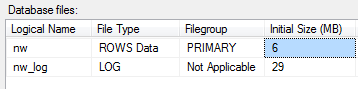
\includegraphics[width=0.75\linewidth,height=\textheight,keepaspectratio]{./images/img-110-076.png}

Bármilyen kimenet adatbázis-sérülést jelez.

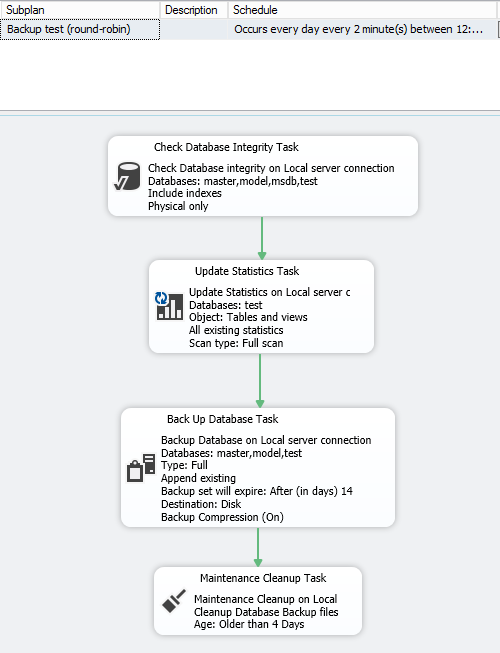
\includegraphics[width=0.75\linewidth,height=\textheight,keepaspectratio]{./images/img-112-077.png}

\begin{center}\rule{0.5\linewidth}{0.5pt}\end{center}

\subsection{Adatbázis-teljesítmény}\label{adatbuxe1zis-teljesuxedtmuxe9ny}

Válaszd ki a megfelelő helyreállítási módot (recovery mode). A FULL
módot csak akkor használd, ha az alkalmazás valóban megköveteli. Győződj
meg arról, hogy az alábbi adatbázis-beállítások helyesek:

\begin{itemize}
\tightlist
\item
  \textbf{Auto update statistics} = TRUE
\item
  \textbf{Auto create statistics} = TRUE
\item
  \textbf{Auto shrink} = FALSE (lehetőség szerint a tábla- és
  adatbázis-zsugorítást egyáltalán ne használd)
\item
  \textbf{Page verify} = CHECKSUM
\end{itemize}

Az adatbázis finomhangolása egy adott alkalmazáshoz nem tartozik ennek a
kurzusnak a hatókörébe.

\begin{center}\rule{0.5\linewidth}{0.5pt}\end{center}

\subsection{Biztonsági mentések}\label{biztonsuxe1gi-mentuxe9sek}

Kliens-szerver adatbázis-alkalmazásban az előre-írás (write-ahead)
tranzakciós naplóval védekezünk az adatveszteség ellen. Három típusú
hibára kell felkészülni:

\begin{enumerate}
\def\labelenumi{\arabic{enumi}.}
\tightlist
\item
  A klienssel megszakad a kapcsolat → a napló segítségével
  visszagörgetjük az összes nem véglegesített tranzakciót.
\item
  A szerver folyamata leáll (elvész a memóriabeli adat és naplópuffer) →
  újraindításkor a szerver először előre görget minden olyan
  tranzakciólépést, amelynek adatlapjai még nem kerültek a fájlba, majd
  visszagörgeti az összes nem véglegesített tranzakciót.
\item
  Az adatfájl elveszik → mentjük a tranzakciós naplót, a korábbi teljes
  és differenciális mentések, majd a naplómentés segítségével
  visszaállítjuk az adatbázist, végül visszagörgetjük a nem
  véglegesített tranzakciókat.
\end{enumerate}

A rendszeres biztonsági mentés a legáltalánosabb katasztrófa-elhárítási
módszer. A mentési fájlokat az adatbázis adatfájljaitól és
naplófájljaitól eltérő adathordozón kell tárolni. A három leggyakoribb
stratégia:

\begin{itemize}
\tightlist
\item
  \textbf{\#1 -- Minimum:} teljes mentések SIMPLE helyreállítási
  módban\footnote{A SIMPLE helyreállítási mód azt jelenti, hogy a napló
    inaktív részei rendszeresen csonkolásra kerülnek.}, pl. naponta
  egyszer, terhelésmentes időszakban. A mentéseket körforgásosan tárold
  (pl. heti ciklusban). Az adatveszteség így legfeljebb egy napra
  korlátozható. Érdemes a \texttt{master}, \texttt{model} és
  \texttt{msdb} adatbázisokat is belefoglalni.
\item
  \textbf{\#2:} Teljes mentések és differenciális mentések SIMPLE
  helyreállítási módban, pl. napi teljes mentés és 2 óránkénti
  differenciális mentés. Az adatveszteség legfeljebb 2 órára
  korlátozható.
\item
  \textbf{\#3:} Ha az alkalmazás minimális adatveszteséget követel meg,
  az adatbázist FULL helyreállítási módba kell állítani, és a 2.
  stratégiát tranzakciósnapló-mentésekkel kell kiegészíteni. FULL módban
  mentések nélkül a napló jelentősen megnőhet. Példastratégia: napi
  teljes mentés, 2 óránkénti differenciális mentés, 20 percenkénti
  tranzakciósnapló-mentés. Ha az adatfájl elveszik, az összes
  véglegesített tranzakció megőrzhető.
\end{itemize}

A mentések a \texttt{BACKUP\ DATABASE} / \texttt{RESTORE\ DATABASE}
T-SQL utasításokkal végezhetők:\footnote{Az SQL-szkriptek az SSMS minden
  párbeszédpaneljéről generálhatók.}

\begin{Shaded}
\begin{Highlighting}[]
\KeywordTok{USE}\NormalTok{ [}\KeywordTok{master}\NormalTok{]}
\NormalTok{RESTORE }\KeywordTok{DATABASE}\NormalTok{ [northwind] }\KeywordTok{FROM}\NormalTok{ DISK }\OperatorTok{=}\NormalTok{ N}\StringTok{\textquotesingle{}C:\textbackslash{}Program Files\textbackslash{}Microsoft SQL}
\StringTok{Server\textbackslash{}MSSQL14.PRIM\textbackslash{}MSSQL\textbackslash{}Backup}\CharTok{\textbackslash{}n}\StringTok{w\textquotesingle{}} \KeywordTok{WITH} \KeywordTok{FILE} \OperatorTok{=} \DecValTok{1}\NormalTok{, NOUNLOAD, }\KeywordTok{REPLACE}\NormalTok{, STATS }\OperatorTok{=} \DecValTok{5}
\end{Highlighting}
\end{Shaded}

\begin{quote}
\textbf{GYAKORLAT:} szimuláljuk a lemezhiba-helyreállítást. Hozz létre
teljes biztonsági mentést a Northwind adatbázisról egy fájleszközre,
állítsd le a PRIM SQL Server-szolgáltatást, töröld az adatbázisfájlt,
indítsd el újra a szolgáltatást, majd állítsd vissza a mentésből a
\texttt{WITH\ REPLACE} opcióval. Ellenőrizd a tartalmat.
\end{quote}

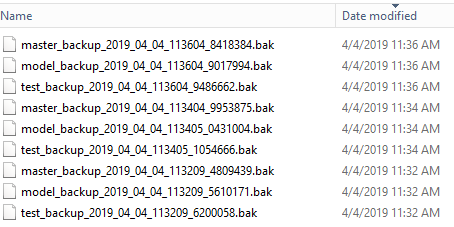
\includegraphics[width=0.75\linewidth,height=\textheight,keepaspectratio]{./images/img-113-078.png}

Rendszeres mentéshez az egyik lehetőség a \texttt{BACKUP} T-SQL
utasítást ütemezett jobban futtatni. A másik lehetőség karbantartási
tervbe (maintenance plan) integrálni a mentési jobokat.

\begin{center}\rule{0.5\linewidth}{0.5pt}\end{center}

\subsection{Karbantartási tervek}\label{karbantartuxe1si-tervek}

A terv létrehozása előtt engedélyezni kell az SQL Server Agent
kiterjesztett tárolt eljárásainak (XPs) használatát:

\begin{Shaded}
\begin{Highlighting}[]
\KeywordTok{use} \KeywordTok{master}
\NormalTok{sp\_configure }\StringTok{\textquotesingle{}show advanced options\textquotesingle{}}\NormalTok{, }\DecValTok{1}
\NormalTok{go}
\NormalTok{reconfigure}
\NormalTok{go}
\NormalTok{sp\_configure }\StringTok{\textquotesingle{}Agent XPs\textquotesingle{}}\NormalTok{, }\DecValTok{1}
\NormalTok{go}
\NormalTok{reconfigure}
\NormalTok{go}
\end{Highlighting}
\end{Shaded}

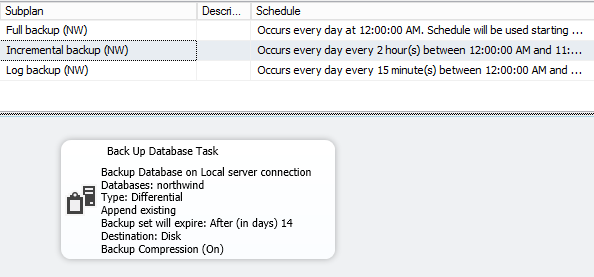
\includegraphics[width=0.75\linewidth,height=\textheight,keepaspectratio]{./images/img-113-079.png}

\begin{quote}
\textbf{GYAKORLAT:} valósítsd meg az \#1 biztonsági mentési stratégiát
egy új karbantartási tervben egy új tesztadatbázishoz. Az ütemezést
állítsd 2 percre (csak a bemutatóhoz). Foglalja magában az indexek
újraszámítását és az integritás-ellenőrzést is napi feladatként.
Használd a \textbf{Management → Maintenance Plans} menüpontot --- ne a
varázslót. Ellenőrizd, hogy 2 percenként jönnek-e létre a mentési
fájlok.
\end{quote}

A törlési (cleanup) feladatot nem tudjuk tesztelni, mert a minimális
törlési kor 1 napnál kevesebbre nem állítható.

\begin{quote}
\textbf{GYAKORLAT:} valósítsd meg a \#3 biztonsági mentési stratégiát
egy új karbantartási tervben a Northwind adatbázishoz.
\end{quote}

\begin{center}\rule{0.5\linewidth}{0.5pt}\end{center}

\subsection{Riasztások (Alerts)}\label{riasztuxe1sok-alerts}

Célszerű riasztást beállítani minden 24-es súlyosságú (severity 24)
hibára. Egy másik klasszikus kritikus feltétel, ha az adatbázisfájlokat
tartalmazó köteten kevés a szabad terület.

\begin{quote}
\textbf{DEMO:} beállítunk egy riasztást, amely akkor aktiválódik, ha a
Northwind adatbázis mérete eléri a jelenlegi méret 150\%-át. Előbb
ellenőrizd az aktuális méretet a
\texttt{C:\textbackslash{}Program\ Files\textbackslash{}Microsoft\ SQL\ Server\textbackslash{}MSSQL14.PRIM\textbackslash{}MSSQL\textbackslash{}DATA}
mappában: 8,2 MB.
\end{quote}

Ha a méret lényegesen nagyobb, állítsd SIMPLE helyreállítási módba, majd
zsugorítsd az adatbázist, 10\%-os szabad helyet hagyva:

\begin{Shaded}
\begin{Highlighting}[]
\KeywordTok{use} \KeywordTok{master}
\NormalTok{dbcc shrinkdatabase(northwind, }\DecValTok{10}\NormalTok{)}
\end{Highlighting}
\end{Shaded}

A riasztás beállítása 4 lépésből áll:

\begin{enumerate}
\def\labelenumi{\arabic{enumi}.}
\tightlist
\item
  Adatbázis-levelezési profil (Database Mail profile) beállítása
\item
  A levelezési profil engedélyezése az SQL Server Agentben
\item
  Operátor létrehozása (az a személy, aki megkapja a riasztást és kezeli
  a problémát)
\item
  A riasztás létrehozása és tesztelése
\end{enumerate}

\subsubsection{Adatbázis-levelezés
beállítása}\label{adatbuxe1zis-levelezuxe9s-beuxe1lluxedtuxe1sa}

Válaszd a \textbf{Server → Management → Database Mail → Configure
Database Mail} lehetőséget. Az új profil panelen írd be a profil nevét:
\texttt{prim\_mail}, majd kattints az \textbf{Add SMTP account} gombra,
és add meg az SMTP-szerver nevét. Tedd a profilt nyilvánossá, hogy
minden felhasználó küldhessen vele e-mailt.

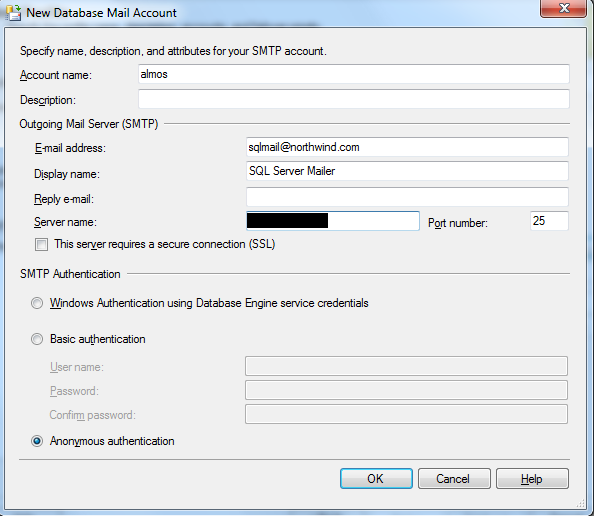
\includegraphics[width=0.75\linewidth,height=\textheight,keepaspectratio]{./images/img-114-080.png}

Ellenőrizd a profil működését: \textbf{Database Mail → Send test
E-mail}.

\subsubsection{Az operátor
létrehozása}\label{az-operuxe1tor-luxe9trehozuxe1sa}

Válaszd az SQL Server Agent csomópont \textbf{Operators} elemét, adj
hozzá egy új operátort, és az \textbf{E-mail name} mezőbe írd be a saját
e-mail-címedet.

\subsubsection{A riasztás
hozzáadása}\label{a-riasztuxe1s-hozzuxe1aduxe1sa}

Válaszd az SQL Server Agent csomópont \textbf{Alerts} elemét, és adj
hozzá egy új riasztást. Állítsd be a választ: \textbf{Notify operator
(NW system administrator) by email}. Az \textbf{Options} lapon adj hozzá
egyéni üzenetet, és állítsd a késleltetést 1 percre (csak a
bemutatóhoz).

Teszteld a riasztást az alábbi szkripttel:

\begin{Shaded}
\begin{Highlighting}[]
\KeywordTok{select}
\NormalTok{  object\_name(object\_id) }\KeywordTok{as} \StringTok{\textquotesingle{}tablename\textquotesingle{}}\NormalTok{,}
  \FunctionTok{count}\NormalTok{(}\OperatorTok{*}\NormalTok{) }\KeywordTok{as} \StringTok{\textquotesingle{}totalpages\textquotesingle{}}\NormalTok{,}
  \FunctionTok{sum}\NormalTok{(}\ControlFlowTok{Case} \ControlFlowTok{when}\NormalTok{ is\_allocated}\OperatorTok{=}\DecValTok{0} \ControlFlowTok{then} \DecValTok{1} \ControlFlowTok{else} \DecValTok{0} \ControlFlowTok{end}\NormalTok{) }\KeywordTok{as} \StringTok{\textquotesingle{}unusedPages\textquotesingle{}}\NormalTok{,}
  \FunctionTok{sum}\NormalTok{(}\ControlFlowTok{Case} \ControlFlowTok{when}\NormalTok{ is\_allocated}\OperatorTok{=}\DecValTok{1} \ControlFlowTok{then} \DecValTok{1} \ControlFlowTok{else} \DecValTok{0} \ControlFlowTok{end}\NormalTok{) }\KeywordTok{as} \StringTok{\textquotesingle{}usedPages\textquotesingle{}}
\KeywordTok{from}\NormalTok{ sys.dm\_db\_database\_page\_allocations(db\_id(),}\KeywordTok{null}\NormalTok{,}\KeywordTok{null}\NormalTok{,}\KeywordTok{null}\NormalTok{,}\StringTok{\textquotesingle{}DETAILED\textquotesingle{}}\NormalTok{)}
\KeywordTok{group} \KeywordTok{by}
\NormalTok{  object\_name(object\_id)}

\CommentTok{{-}{-}létrehozunk egy nagy táblát}
\NormalTok{go}
\KeywordTok{create} \KeywordTok{table}\NormalTok{ big\_table (a }\DataTypeTok{char}\NormalTok{(}\DecValTok{4000}\NormalTok{))}
\KeywordTok{declare}\NormalTok{ @i }\DataTypeTok{int}\OperatorTok{=}\DecValTok{0}
\ControlFlowTok{while}\NormalTok{ @i}\OperatorTok{\textless{}}\DecValTok{1000} \ControlFlowTok{begin}
  \KeywordTok{insert}\NormalTok{ big\_table }\KeywordTok{values}\NormalTok{ (}\StringTok{\textquotesingle{}a\textquotesingle{}}\NormalTok{)}
  \KeywordTok{set}\NormalTok{ @i}\OperatorTok{=}\NormalTok{@i}\OperatorTok{+}\DecValTok{1}
\ControlFlowTok{end}
\CommentTok{{-}{-}a big\_table 500 lapos {-}\textgreater{} a riasztás elsül}
\end{Highlighting}
\end{Shaded}

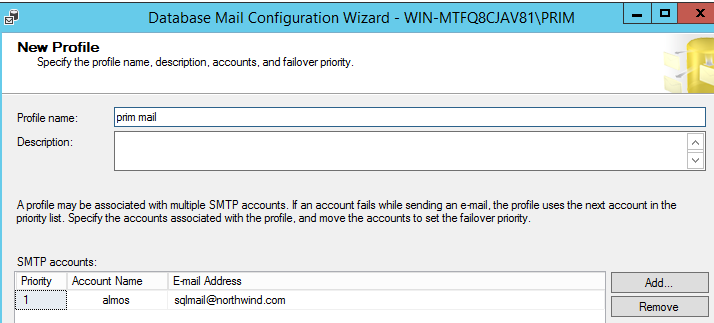
\includegraphics[width=0.75\linewidth,height=\textheight,keepaspectratio]{./images/img-115-081.png}

Ellenőrizd a riasztás előzményeit és a postaládádat. Ne felejtsd el
törölni a \texttt{big\_table}-t, és letiltani vagy törölni a riasztást.

\begin{center}\rule{0.5\linewidth}{0.5pt}\end{center}

\subsection{Rendszerbiztonsági tagok, jogosultságok, sémák,
szerepkörök}\label{rendszerbiztonsuxe1gi-tagok-jogosultsuxe1gok-suxe9muxe1k-szerepkuxf6ruxf6k}

A kiszolgálói bejelentkezések (login) és az adatbázis-felhasználók
(database user) viszonyának áttekintése. A bejelentkezés
adatbázis-felhasználókhoz kapcsolódik, és általában van alapértelmezett
adatbázisa.

\begin{Shaded}
\begin{Highlighting}[]
\KeywordTok{use} \KeywordTok{master}
\KeywordTok{create}\NormalTok{ login nw\_user }\KeywordTok{with} \KeywordTok{password}\OperatorTok{=}\StringTok{\textquotesingle{}...\textquotesingle{}}\NormalTok{, default\_database}\OperatorTok{=}\NormalTok{northwind}
\KeywordTok{use}\NormalTok{ northwind }\CommentTok{{-}{-}context switch}
\KeywordTok{create} \FunctionTok{user}\NormalTok{ nw\_user }\ControlFlowTok{for}\NormalTok{ login nw\_user}
\KeywordTok{alter} \KeywordTok{role}\NormalTok{ db\_datareader }\KeywordTok{add} \KeywordTok{member}\NormalTok{ nw\_user}
\end{Highlighting}
\end{Shaded}

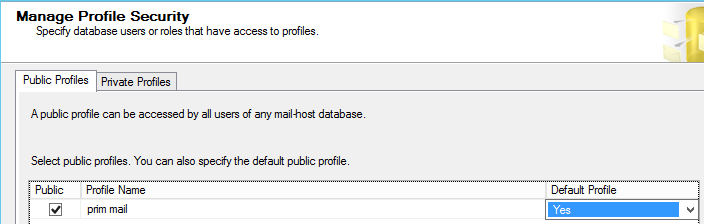
\includegraphics[width=0.75\linewidth,height=\textheight,keepaspectratio]{./images/img-115-082.png}

\begin{quote}
\textbf{GYAKORLAT:} hozz létre egy új adatbázist, egy új bejelentkezést
és egy új adatbázis-felhasználót.
\end{quote}

A jogosultságok áttekintése:
\texttt{GRANT\ {[}jogosultság{]}\ ON\ {[}objektum{]}\ TO\ {[}kinek{]}},
\texttt{REVOKE}, \texttt{DENY}.

\begin{Shaded}
\begin{Highlighting}[]
\KeywordTok{use}\NormalTok{ northwind}
\KeywordTok{alter} \KeywordTok{role}\NormalTok{ db\_datareader }\KeywordTok{drop} \KeywordTok{member}\NormalTok{ nw\_user}
\NormalTok{go}
\KeywordTok{create} \KeywordTok{procedure}\NormalTok{ sp\_list\_employees}
\NormalTok{  @city }\DataTypeTok{varchar}\NormalTok{(}\DecValTok{50}\NormalTok{) }\OperatorTok{=} \StringTok{\textquotesingle{}London\textquotesingle{}} \CommentTok{{-}{-}a paraméter alapértelmezett értéke}
\KeywordTok{as}
  \KeywordTok{select} \OperatorTok{*} \KeywordTok{from}\NormalTok{ Employees }\KeywordTok{where}\NormalTok{ City}\OperatorTok{=}\NormalTok{@city}
\NormalTok{go}
\KeywordTok{exec}\NormalTok{ sp\_list\_employees}
\NormalTok{go}
\KeywordTok{exec}\NormalTok{ sp\_list\_employees }\StringTok{\textquotesingle{}Seattle\textquotesingle{}}
\NormalTok{go}
\KeywordTok{grant} \KeywordTok{execute} \KeywordTok{on}\NormalTok{ sp\_list\_employees }\KeywordTok{to}\NormalTok{ nw\_user}
\NormalTok{go}
\end{Highlighting}
\end{Shaded}

A szerepkörök (roles) jogosultságcsoportok, pl. olvasási hozzáférés
minden táblához.

Fontos \textbf{kiszolgáló szintű szerepkörök}: \texttt{public},
\texttt{dbcreator}, \texttt{serveradmin}, \texttt{sysadmin}

Fontos \textbf{adatbázisszintű szerepkörök}: \texttt{db\_owner},
\texttt{db\_datareader}, \texttt{db\_datawriter}; tiltó szerepkörök:
\texttt{db\_denydatawriter}, \texttt{db\_denydatareader}

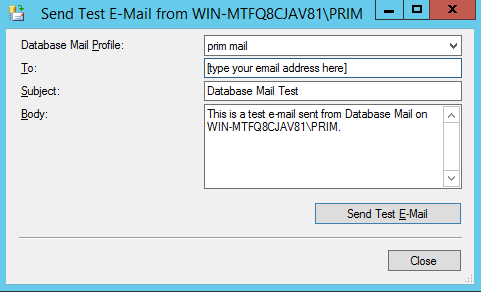
\includegraphics[width=0.75\linewidth,height=\textheight,keepaspectratio]{./images/img-115-083.png}

\begin{Shaded}
\begin{Highlighting}[]
\KeywordTok{use}\NormalTok{ adworks}
\KeywordTok{alter} \KeywordTok{role}\NormalTok{ exec\_all\_sp }\KeywordTok{drop} \KeywordTok{member}\NormalTok{ nw\_user}
\KeywordTok{alter} \KeywordTok{role}\NormalTok{ db\_owner }\KeywordTok{add} \KeywordTok{member}\NormalTok{ nw\_user}
\KeywordTok{alter} \KeywordTok{role}\NormalTok{ db\_denydatawriter }\KeywordTok{add} \KeywordTok{member}\NormalTok{ nw\_user}

\CommentTok{{-}{-}ellenőrzés egy nw\_user kliens{-}kapcsolatban:}
\KeywordTok{use}\NormalTok{ adworks}
\KeywordTok{select} \OperatorTok{*} \KeywordTok{from}\NormalTok{ Sales.}\KeywordTok{Store}
\CommentTok{{-}{-}(701 sort érint)}
\KeywordTok{exec}\NormalTok{ Person.sp\_DeletePerson\_Temporal }\DecValTok{2}
\CommentTok{{-}{-}(1 sort érint)}
\CommentTok{{-}{-}(1 sort érint)}
\KeywordTok{create} \KeywordTok{table}\NormalTok{ test (}\KeywordTok{id} \DataTypeTok{int}\NormalTok{)}
\CommentTok{{-}{-}A parancsok sikeresen lefutottak.}
\KeywordTok{insert}\NormalTok{ test (}\KeywordTok{id}\NormalTok{) }\KeywordTok{values}\NormalTok{ (}\DecValTok{25}\NormalTok{)}
\CommentTok{{-}{-}Msg 229, Level 14, State 5, Line 10}
\CommentTok{{-}{-}Az INSERT jogosultságot megtagadta a \textquotesingle{}test\textquotesingle{} objektum, \textquotesingle{}adworks\textquotesingle{} adatbázis, \textquotesingle{}dbo\textquotesingle{} séma esetén.}
\KeywordTok{drop} \KeywordTok{table}\NormalTok{ test}
\CommentTok{{-}{-}A parancsok sikeresen lefutottak.}
\end{Highlighting}
\end{Shaded}

Saját szerepkörök is létrehozhatók:

\begin{Shaded}
\begin{Highlighting}[]
\KeywordTok{use}\NormalTok{ northwind}
\KeywordTok{revoke} \KeywordTok{execute} \KeywordTok{on}\NormalTok{ sp\_list\_employees }\KeywordTok{from}\NormalTok{ nw\_user}
\NormalTok{go}
\CommentTok{{-}{-}így adható végrehajtási jog az adatbázis ÖSSZES objektumára}
\KeywordTok{grant} \KeywordTok{execute} \KeywordTok{to}\NormalTok{ nw\_user}

\CommentTok{{-}{-}új szerepkör}
\KeywordTok{use}\NormalTok{ adworks}
\KeywordTok{create} \KeywordTok{role}\NormalTok{ exec\_all\_sp}
\KeywordTok{grant} \KeywordTok{execute} \KeywordTok{on} \KeywordTok{schema}\NormalTok{:}\CharTok{:Person} \KeywordTok{to}\NormalTok{ exec\_all\_sp }\CommentTok{{-}{-}a szerepkör rendszerbiztonsági tagként viselkedik}
\CommentTok{{-}{-}alternatíva lehet: grant select, update on schema::Person to read\_update\_only\_role stb.}
\KeywordTok{create} \FunctionTok{user}\NormalTok{ nw\_user }\ControlFlowTok{for}\NormalTok{ login nw\_user}
\KeywordTok{alter} \KeywordTok{role}\NormalTok{ exec\_all\_sp }\KeywordTok{add} \KeywordTok{member}\NormalTok{ nw\_user}

\CommentTok{{-}{-}ellenőrzés egy kliens{-}kapcsolatban}
\KeywordTok{use}\NormalTok{ adworks}
\KeywordTok{select} \OperatorTok{*} \KeywordTok{from}\NormalTok{ Sales.}\KeywordTok{Store}
\CommentTok{{-}{-}Msg 229, Level 14, State 5, Line 8}
\CommentTok{{-}{-}A SELECT jogosultságot megtagadta a \textquotesingle{}Store\textquotesingle{} objektum, \textquotesingle{}adworks\textquotesingle{} adatbázis, \textquotesingle{}Sales\textquotesingle{} séma esetén.}
\KeywordTok{exec}\NormalTok{ Person.sp\_DeletePerson\_Temporal }\DecValTok{2}
\CommentTok{{-}{-}(1 sort érint)}
\CommentTok{{-}{-}(1 sort érint)}
\end{Highlighting}
\end{Shaded}

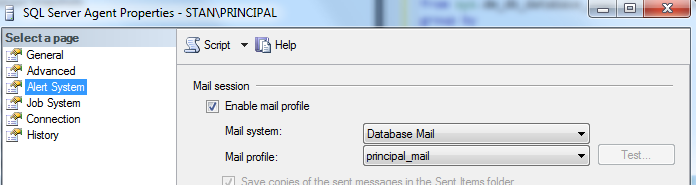
\includegraphics[width=0.75\linewidth,height=\textheight,keepaspectratio]{./images/img-116-084.png}

\begin{quote}
\textbf{GYAKORLAT:} hozz létre egy új szerepkört a
\texttt{db\_datareader} és \texttt{db\_datawriter} szerepkörök
összeolvasztásaként, és rendeld hozzá az új felhasználót. Teszteld.
\end{quote}

Az adatbázis-objektumok egy sémához tartoznak, és a sémának egyetlen
tulajdonosa van (ez különbözik a \texttt{db\_owner} adatbázisszerepkör
tagságától). A tulajdonos ejthet (DROP) sémát, és létrehozhat, illetve
törölhet objektumokat a sémában. A jogosultságokat általában
séma/szerepkör szinten, nem egyedi felhasználó/tábla szinten kezeljük.

Melyik rendszerbiztonsági tag melyik szerepkörben van?

\begin{Shaded}
\begin{Highlighting}[]
\KeywordTok{select}\NormalTok{ DP1.name }\KeywordTok{as}\NormalTok{ DatabaseRoleName, isnull (DP2.name, }\StringTok{\textquotesingle{}No members\textquotesingle{}}\NormalTok{) }\KeywordTok{as}
\NormalTok{DatabaseUserName}
\KeywordTok{from}\NormalTok{ sys.database\_role\_members }\KeywordTok{as}\NormalTok{ DRM }\KeywordTok{right} \KeywordTok{outer} \KeywordTok{join}
\NormalTok{sys.database\_principals }\KeywordTok{as}\NormalTok{ DP1 }\KeywordTok{on}\NormalTok{ DRM.role\_principal\_id }\OperatorTok{=}\NormalTok{ DP1.principal\_id }\KeywordTok{left} \KeywordTok{outer}
\KeywordTok{join}\NormalTok{ sys.database\_principals }\KeywordTok{as}\NormalTok{ DP2 }\KeywordTok{on}\NormalTok{ DRM.member\_principal\_id }\OperatorTok{=}\NormalTok{ DP2.principal\_id}
\KeywordTok{where}\NormalTok{ DP1.}\KeywordTok{type} \OperatorTok{=} \StringTok{\textquotesingle{}R\textquotesingle{}} \CommentTok{{-}{-}R: adatbázis{-}szerepkör}
\KeywordTok{order} \KeywordTok{by}\NormalTok{ DP1.name}
\end{Highlighting}
\end{Shaded}

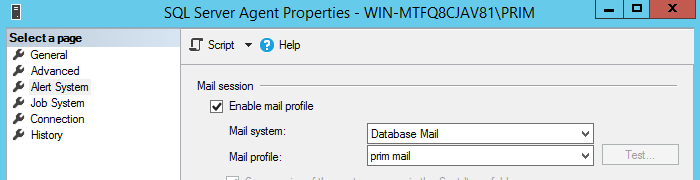
\includegraphics[width=0.75\linewidth,height=\textheight,keepaspectratio]{./images/img-116-085.png}

\begin{quote}
\textbf{GYAKORLAT:} tervezd meg egy nagy nemzeti könyvtár (pl. OSzK)
sémáit, szerepköreit és jogosultságait.
\end{quote}

\begin{center}\rule{0.5\linewidth}{0.5pt}\end{center}

\subsection{Adatbiztonság az SQL
Serverben}\label{adatbiztonsuxe1g-az-sql-serverben}

\subsubsection{Érzékeny adatok
osztályozása}\label{uxe9rzuxe9keny-adatok-osztuxe1lyozuxe1sa}

Az SQL Server 2017-től a mezők automatikusan vagy manuálisan
osztályozhatók információtípus (pl. „Personal'') és érzékenységi szint
(pl. „Confidential-GDPR'') szerint. Használd a \textbf{Database → Tasks
→ Classify data} eszközt. A rendszer sebezhetőségi elemzést
(vulnerability analysis) is futtathat.

Az adatbiztonság területei:

\begin{itemize}
\tightlist
\item
  \textbf{Biztonságos ügyfélkapcsolatok} → SSL. A szerverhez telepíteni
  kell egy tanúsítványt.
\item
  \textbf{Adatbázis- és mentési fájlok} (data at rest):

  \begin{itemize}
  \tightlist
  \item
    Fájlszint: mentési titkosítás (backup encryption) és transzparens
    adattitkosítás (TDE), amely az adatfájlokat is titkosítja.
  \item
    Mezőszint: érzékeny oszlopok elrejtése még a \texttt{sysadmin}
    szerepkör elől is („Always Encrypted''), titkosítással és
    visszafejtéssel a kliensoldali.
  \end{itemize}
\item
  \textbf{A szerver által feldolgozott adatok} (data in motion):

  \begin{itemize}
  \tightlist
  \item
    \textbf{Dinamikus adatmaszkolás} (Dynamic Data Masking): érzékeny
    oszlopok részleges elrejtése a sémában definiált maszkkal, pl.
    \texttt{ALTER\ COLUMN\ {[}Social\ Security\ Number{]}\ \textless{}adattípus\textgreater{}\ MASKED\ WITH\ (FUNCTION\ =\ \textquotesingle{}partial(0,"XXX-XX-",4)\textquotesingle{})}
    --- csak az utolsó 4 jegy látható. Az \texttt{UNMASK} jogosultsággal
    rendelkező felhasználók az eredeti értéket olvashatják.\footnote{https://www.sqlshack.com/using-dynamic-data-masking-in-sql-server-2016-to-protect-sensitive-data/}
  \end{itemize}
\end{itemize}

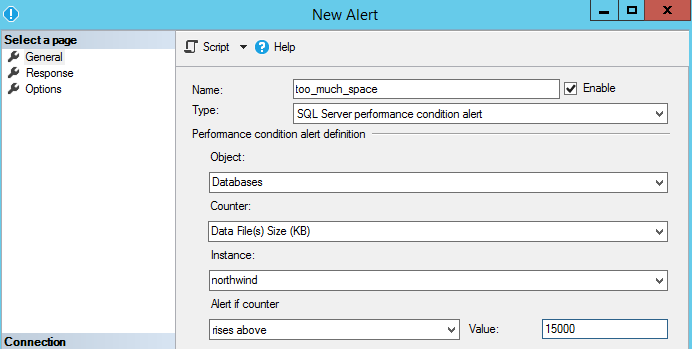
\includegraphics[width=0.75\linewidth,height=\textheight,keepaspectratio]{./images/img-116-086.png}

A javasolt legjobb gyakorlat: az érzékenynek minősített mezőkre
mezőszintű védelmet kell alkalmazni.

\subsubsection{DEMO --- dinamikus
adatmaszkolás}\label{demo-dinamikus-adatmaszkoluxe1s}

\begin{Shaded}
\begin{Highlighting}[]
\KeywordTok{use}\NormalTok{ northwind}
\CommentTok{{-}{-}alter table employees drop column SSN}
\CommentTok{{-}{-}alter table employees drop column email}
\KeywordTok{alter} \KeywordTok{table}\NormalTok{ employees }\KeywordTok{add}\NormalTok{ ssn }\DataTypeTok{char}\NormalTok{(}\DecValTok{10}\NormalTok{) }\KeywordTok{null}\NormalTok{, email }\DataTypeTok{varchar}\NormalTok{(}\DecValTok{200}\NormalTok{) }\CommentTok{{-}{-}érzékeny oszlopok}
\KeywordTok{alter} \KeywordTok{table}\NormalTok{ employees }\KeywordTok{alter} \KeywordTok{column}\NormalTok{ ssn }\DataTypeTok{char}\NormalTok{(}\DecValTok{10}\NormalTok{) masked }\KeywordTok{with}\NormalTok{ (}\KeywordTok{function} \OperatorTok{=}
\StringTok{\textquotesingle{}partial(1,".....",4)\textquotesingle{}}\NormalTok{)}
\KeywordTok{alter} \KeywordTok{table}\NormalTok{ employees }\KeywordTok{alter} \KeywordTok{column}\NormalTok{ email }\DataTypeTok{char}\NormalTok{(}\DecValTok{200}\NormalTok{) masked }\KeywordTok{with}\NormalTok{ (}\KeywordTok{function} \OperatorTok{=} \StringTok{\textquotesingle{}email()\textquotesingle{}}\NormalTok{)}
\NormalTok{go}
\KeywordTok{update}\NormalTok{ Employees }\KeywordTok{set}\NormalTok{ ssn }\OperatorTok{=}\StringTok{\textquotesingle{}1234567890\textquotesingle{}}
\KeywordTok{update}\NormalTok{ Employees }\KeywordTok{set}\NormalTok{ email }\OperatorTok{=}\StringTok{\textquotesingle{}sohase\_mondd@citromail.hu\textquotesingle{}}
\KeywordTok{select}\NormalTok{ lastname, ssn, email }\KeywordTok{from}\NormalTok{ Employees }\CommentTok{{-}{-}minden értéket látunk}

\CommentTok{{-}{-}ha viszont létrehozunk egy írási/olvasási jogú felhasználót}
\KeywordTok{use} \KeywordTok{master}
\KeywordTok{create}\NormalTok{ login test }\KeywordTok{with} \KeywordTok{password}\OperatorTok{=}\StringTok{\textquotesingle{}h6twqPNO\textquotesingle{}}\NormalTok{, default\_database}\OperatorTok{=}\NormalTok{northwind}
\NormalTok{go}
\KeywordTok{use}\NormalTok{ northwind }\CommentTok{{-}{-}context switch}
\KeywordTok{create} \FunctionTok{user}\NormalTok{ test }\ControlFlowTok{for}\NormalTok{ login test}
\KeywordTok{alter} \KeywordTok{role}\NormalTok{ db\_datareader }\KeywordTok{add} \KeywordTok{member}\NormalTok{ test}
\KeywordTok{alter} \KeywordTok{role}\NormalTok{ db\_datawriter }\KeywordTok{add} \KeywordTok{member}\NormalTok{ test}
\NormalTok{go}

\CommentTok{{-}{-}váltsunk át a test felhasználó kapcsolatára}
\KeywordTok{execute} \KeywordTok{as} \FunctionTok{user} \OperatorTok{=} \StringTok{\textquotesingle{}test\textquotesingle{}}
\KeywordTok{select}\NormalTok{ lastname, ssn, email }\KeywordTok{from}\NormalTok{ Employees}
\NormalTok{revert}
\NormalTok{go}
\CommentTok{{-}{-}ezt látjuk:}
\CommentTok{{-}{-}lastname     ssn           email}
\CommentTok{{-}{-}Davolio      1.....7890    sXXX@XXXX.com}
\CommentTok{{-}{-}Fuller       1.....7890    sXXX@XXXX.com}

\CommentTok{{-}{-}most adjuk meg az UNMASK jogosultságot a test felhasználónak}
\KeywordTok{grant}\NormalTok{ UNMASK }\KeywordTok{to}\NormalTok{ test}
\NormalTok{go}
\KeywordTok{execute} \KeywordTok{as} \FunctionTok{user} \OperatorTok{=} \StringTok{\textquotesingle{}test\textquotesingle{}}
\KeywordTok{select}\NormalTok{ lastname, ssn, email }\KeywordTok{from}\NormalTok{ Employees}
\NormalTok{revert}
\NormalTok{go}
\CommentTok{{-}{-}most ezt látjuk:}
\CommentTok{{-}{-}lastname     ssn           email}
\CommentTok{{-}{-}Davolio      1234567890    sohase\_mondd@citromail.hu}
\CommentTok{{-}{-}Fuller       1234567890    sohase\_mondd@citromail.hu}

\CommentTok{{-}{-}FIGYELEM: a felhasználó továbbra is módosíthatja az oszlopokat!!!}
\NormalTok{go}
\KeywordTok{execute} \KeywordTok{as} \FunctionTok{user} \OperatorTok{=} \StringTok{\textquotesingle{}test\textquotesingle{}}
\KeywordTok{update}\NormalTok{ Employees }\KeywordTok{set}\NormalTok{ email }\OperatorTok{=}\StringTok{\textquotesingle{}mondj\_igent@citromail.hu\textquotesingle{}}
\KeywordTok{select}\NormalTok{ lastname, ssn, email }\KeywordTok{from}\NormalTok{ Employees}
\NormalTok{revert}
\NormalTok{go}
\KeywordTok{revoke}\NormalTok{ UNMASK }\KeywordTok{from}\NormalTok{ test}
\end{Highlighting}
\end{Shaded}

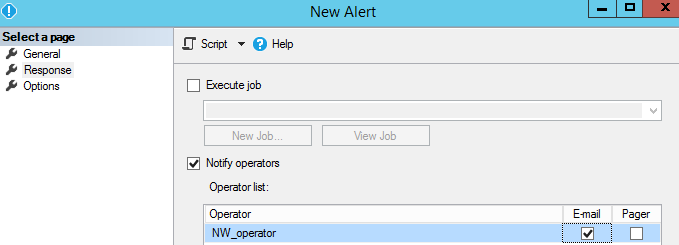
\includegraphics[width=0.75\linewidth,height=\textheight,keepaspectratio]{./images/img-117-087.png}

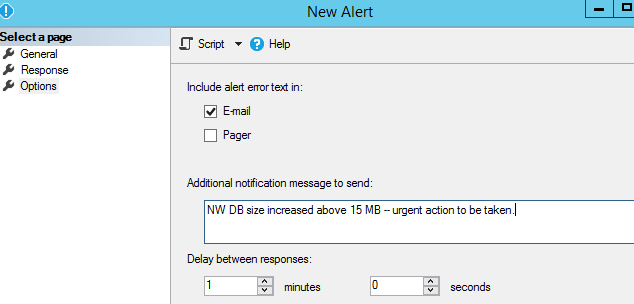
\includegraphics[width=0.75\linewidth,height=\textheight,keepaspectratio]{./images/img-117-088.png}

\begin{quote}
\textbf{GYAKORLAT:} próbáld ki a \texttt{default()} és \texttt{random()}
maszkolási függvényeket az \texttt{AdventureworksDW2019.dbo.DimCustomer}
táblán.
\end{quote}

\begin{center}\rule{0.5\linewidth}{0.5pt}\end{center}

\subsection{SSL konfigurálása}\label{ssl-konfiguruxe1luxe1sa}

\begin{itemize}
\tightlist
\item
  Hozz létre egy új önaláírt tanúsítványt:
  \texttt{certreq\ -new\ -f\ certparam.inf\ local.cer}, az \texttt{.inf}
  fájlban a paraméterek beállításával.
\item
  Az mmc konzolon válaszd az \textbf{All tasks → Manage private keys}
  lehetőséget, és add hozzá az \texttt{MSSQL\$PRIM} felhasználót teljes
  ellenőrzési joggal a tanúsítvány privát kulcsára.
\item
  Az SQL Server Configuration Managerben a \textbf{Protocols →
  Properties} panelen állítsd be az \textbf{Enforce encryption}
  beállítást, majd indítsd újra a szolgáltatást.
\item
  Az SSMS-ben futtasd a
  \texttt{select\ *\ from\ sys.dm\_exec\_connections} lekérdezést, és
  ellenőrizd: \texttt{encrypt\_option=TRUE} → SSL,
  \texttt{auth\_scheme=SQL}.
\end{itemize}

\begin{center}\rule{0.5\linewidth}{0.5pt}\end{center}

\subsection{Mentési titkosítás (Backup
Encryption)}\label{mentuxe9si-titkosuxedtuxe1s-backup-encryption}

A Service Master Key (SMK) az SQL Server-példány telepítésekor
automatikusan jön létre. A mentések titkosításához szükség van egy
\texttt{master} adatbázisban tárolt főkulcsra (Master Key), amelyet a
megadott jelszóval és az SMK-val is titkosítunk. Ez a főkulcs titkosítja
a mentési tanúsítványok privát kulcsait.\footnote{https://docs.microsoft.com/en-us/sql/relational-databases/backup-restore/backup-encryption?view=sql-server-2017}

\begin{Shaded}
\begin{Highlighting}[]
\KeywordTok{use} \KeywordTok{master}
\KeywordTok{CREATE} \KeywordTok{MASTER} \KeywordTok{KEY}\NormalTok{ ENCRYPTION }\KeywordTok{BY} \KeywordTok{PASSWORD} \OperatorTok{=} \StringTok{\textquotesingle{}h6twqPNO\textquotesingle{}}
\NormalTok{go}
\CommentTok{{-}{-}mentés készítése az új MK{-}ról}
\KeywordTok{OPEN} \KeywordTok{MASTER} \KeywordTok{KEY}\NormalTok{ DECRYPTION }\KeywordTok{BY} \KeywordTok{PASSWORD} \OperatorTok{=} \StringTok{\textquotesingle{}h6twqPNO\textquotesingle{}}
\NormalTok{go}
\CommentTok{{-}{-}a mentéshez eltérő jelszót használunk}
\KeywordTok{BACKUP} \KeywordTok{MASTER} \KeywordTok{KEY} \KeywordTok{TO} \KeywordTok{FILE} \OperatorTok{=} \StringTok{\textquotesingle{}C:\textbackslash{}install}\CharTok{\textbackslash{}e}\StringTok{xportedmasterkey\textquotesingle{}}
\NormalTok{ENCRYPTION }\KeywordTok{BY} \KeywordTok{PASSWORD} \OperatorTok{=} \StringTok{\textquotesingle{}h6twqPNOh6twqPNO\textquotesingle{}}
\NormalTok{go}
\CommentTok{{-}{-}létrehozunk egy privát{-}publikus kulcspárt és egy önaláírt tanúsítványt}
\KeywordTok{CREATE}\NormalTok{ CERTIFICATE backup\_cert\_master}
\CommentTok{{-}{-}ezt az MK fogja titkosítani}
\KeywordTok{WITH}\NormalTok{ SUBJECT }\OperatorTok{=} \StringTok{\textquotesingle{}NW DB backup\textquotesingle{}}\NormalTok{,}
\NormalTok{EXPIRY\_DATE }\OperatorTok{=} \StringTok{\textquotesingle{}20301031\textquotesingle{}}
\KeywordTok{BACKUP}\NormalTok{ CERTIFICATE backup\_cert\_master }\KeywordTok{TO} \KeywordTok{FILE} \OperatorTok{=} \StringTok{\textquotesingle{}C:\textbackslash{}install}\CharTok{\textbackslash{}e}\StringTok{xportedcert\textquotesingle{}}
\CommentTok{{-}{-}visszaállítható a CREATE CERTIFICATE ... paranccsal}
\CommentTok{{-}{-}mentést készítünk az adatbázisról}
\KeywordTok{BACKUP} \KeywordTok{DATABASE}\NormalTok{ northwind }\KeywordTok{TO}\NormalTok{ DISK }\OperatorTok{=} \StringTok{\textquotesingle{}C:\textbackslash{}install}\CharTok{\textbackslash{}n}\StringTok{w\_enc.bak\textquotesingle{}}
\KeywordTok{WITH}\NormalTok{ COMPRESSION, ENCRYPTION (}
\NormalTok{  ALGORITHM }\OperatorTok{=}\NormalTok{ AES\_256,}
\NormalTok{  SERVER CERTIFICATE }\OperatorTok{=}\NormalTok{ backup\_cert\_master}
\NormalTok{), STATS }\OperatorTok{=} \DecValTok{10}
\NormalTok{GO}
\end{Highlighting}
\end{Shaded}

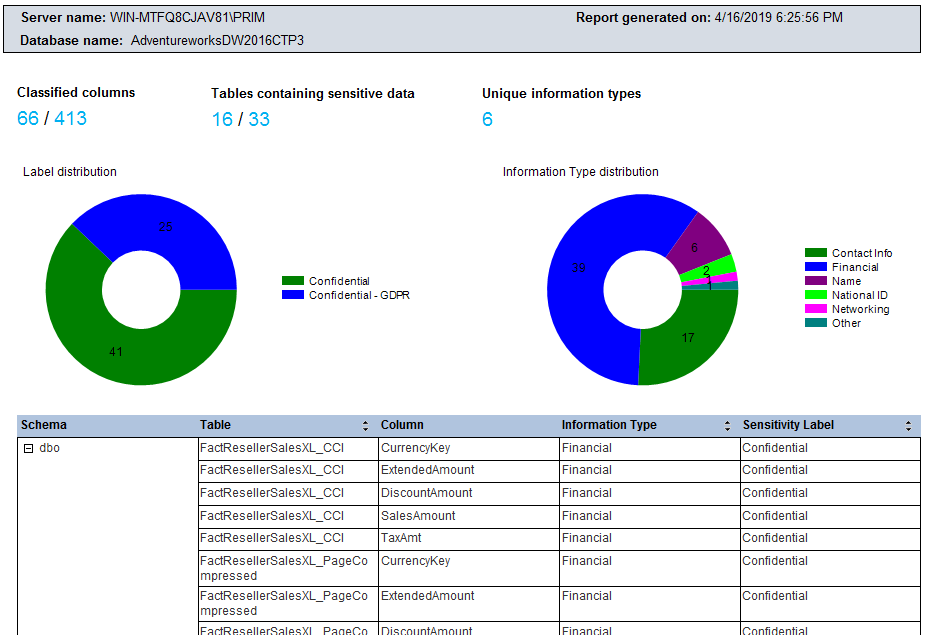
\includegraphics[width=0.75\linewidth,height=\textheight,keepaspectratio]{./images/img-120-089.png}

Próbáld meg a titkosított mentést visszaállítani a PRIM kiszolgálón egy
új adatbázisba (a \texttt{backup\_cert\_master} segítségével
automatikusan visszafejti). Majd próbálj meg ugyanezt elvégezni a SECOND
kiszolgálón --- a mentés tartalma ott olvashatatlan lesz.

\begin{quote}
\textbf{GYAKORLAT:} titkosítsd a tesztadatbázis mentését a főkulccsal,
majd próbáld meg visszaállítani a THIRD kiszolgálón.
\end{quote}

\begin{center}\rule{0.5\linewidth}{0.5pt}\end{center}

\subsection{Always Encrypted}\label{always-encrypted}

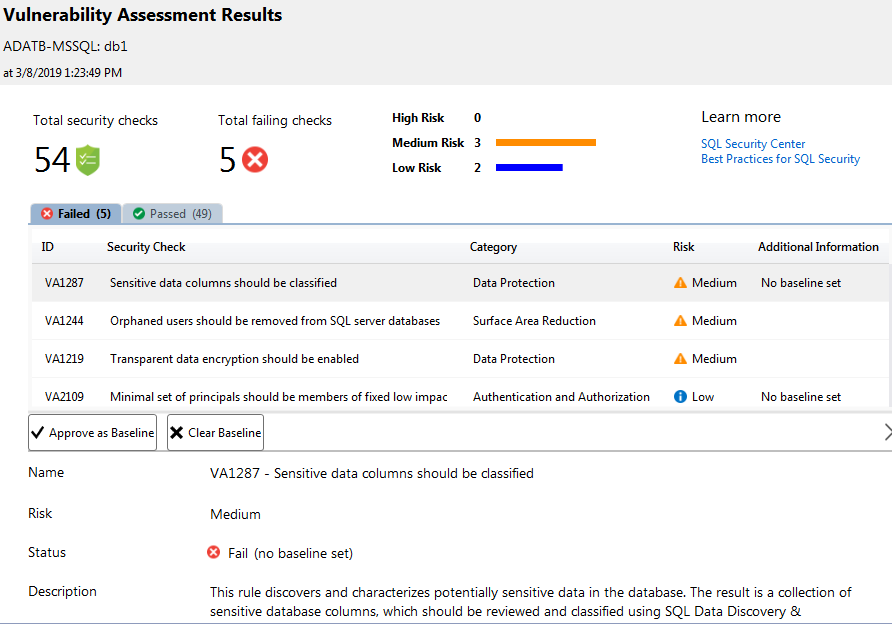
\includegraphics[width=0.75\linewidth,height=\textheight,keepaspectratio]{./images/img-120-090.png}

A titkosítás és visszafejtés a kliensoldali alkalmazásban történik, a
kulcsok az SQL Server-példányon kívül tárolódnak (helyi Windows
tanúsítványtárban vagy Azure Key Vaultban).

\begin{quote}
\textbf{DEMO:} hozzáadjuk az Always Encrypted titkosítást az Employees
tábla Address oszlopához.

\begin{enumerate}
\def\labelenumi{\arabic{enumi}.}
\tightlist
\item
  Válaszd a \textbf{Northwind → Tables → Employees → Encrypt Columns}
  lehetőséget, és jelöld ki az Address mezőt.
\item
  Válaszd a \textbf{Randomized} titkosítási típust. Ez megakadályozza az
  ECB\footnote{https://searchsecurity.techtarget.com/definition/Electronic-Code-Book}-típusú
  támadást, de a titkosított oszlopon nem lehet csoportosítani,
  egyenlőség alapján szűrni vagy JOIN-t futtatni a szerveren.
\item
  Válaszd az új oszlopkulcs generálását.
\item
  Fogadd el, hogy az összevetési sorrend (collation) binárisra változik.
\item
  A következő panelen válaszd a \textbf{Windows certificate store}
  lehetőséget. Ez az SQL Server-példányon kívül van, így az
  \texttt{sysadmin} szerepkörű SQL Server-rendszergazdának nincs
  hozzáférése.
\item
  Ellenőrizd az új tanúsítványt a \texttt{certmgr.msc}
  MMC-alkalmazásban.
\item
  Futtass \texttt{SELECT\ *} lekérdezést a táblán, hogy lásd, mit lát a
  rendszergazda (titkosított értékek).
\item
  A visszafejtett eredmény megtekintéséhez nyiss új kapcsolatot, és az
  \textbf{Options → Additional Connection Parameters} mezőbe írd be:
  \texttt{Column\ Encryption\ Setting\ =\ Enabled}.
\item
  Lekérdezés futtatásakor engedélyezd a paraméterezést
  (parameterization), hogy a titkosított oszlopokba is lehessen szúrni,
  módosítani és szűrni.
\end{enumerate}
\end{quote}

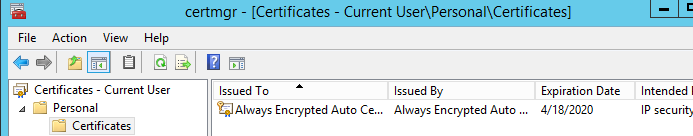
\includegraphics[width=0.75\linewidth,height=\textheight,keepaspectratio]{./images/img-123-091.png}

\begin{quote}
\textbf{GYAKORLAT:} válaszd a \textbf{Deterministic} titkosítási típust
a Title oszlophoz, és ellenőrizd, hogy azonos egyszerű szöveghez azonos
titkosított szöveg generálódik --- ez ECB-típusú támadást tesz lehetővé.
\end{quote}

\begin{center}\rule{0.5\linewidth}{0.5pt}\end{center}

\end{document}
